% \iffalse meta-comment
%<*internal>
\iffalse
%</internal>
%<*readme>
----------------------------------------------------------------
phd-utils --- some useful uitlities
E-mail: yannislaz@gmail.com
Released under the LaTeX Project Public License v1.3c or later
See http://www.latex-project.org/lppl.txt
----------------------------------------------------------------
This file provides package phd-i18n for handling i18n.
%</readme>
%<*readmemd>
###The `phd` LaTeX2e package

The `phd` latex package and the class with the same name provide
convenient methods to create new styles for books, reports
and articles. It also loads the most commonly used packages 
and resolves conflicts.

This work consists of the file  `phd.dtx`,
and the derived files   `phd.ins`,  `phd.pdf`, and `phd.sty`.

The `phd` bundle is a bunch of 15 packages, that manage all
aspects of document production.

They consist of:

1.0  The [phd-pkgmanager](https://github.com/yannisl/phd/blob/master/docs/phd-pkgmanager.md). This
     package manages all aspects of loading numerous packages and avoiding conflicts. It currently
     loads over 100 packages, directly or indirectly.
     
2.0  The [phd-fontmanager](https://github.com/yannisl/phd/blob/master/docs/phd-fontmanager.md). The
     `phd-fontmanager` sets up the fonts to be used for the document and provides an interface to
     all areas where font data is needed.
     
3.0  The [phd-handlers](https://github.com/yannisl/phd/blob/master/docs/phd-handlers.md). As we use
     extensively automatic key generation via code, this package provides numerous handlers.
     
4.0  The [phd-lowerlevelheadings](https://github.com/yannisl/phd/blob/master/docs/phd-lowerlevelheadings.md)     

5.0  The [phd-toc](https://github.com/yannisl/phd/blob/master/docs/phd-toc.md) package.
     Manages all aspects of Table of Contents via a key value interface. 

6.0  The [phd-counters](https://github.com/yannisl/phd/blob/master/docs/phd-counters.md) 

7.0  The [phd-colorpalette](https://github.com/yannisl/phd/blob/master/docs/phd-colorpalette.md). This
     package introduces the concept of a `color palette` to `LaTeX` coding. It groups all color
     data into `palettes`. By setting a single set of keys, the document can be updated with new
     color information.

8.0  The [phd-scriptsmanager](https://github.com/yannisl/phd/blob/master/docs/phd-scriptsmanager.md).
     Handles the settings and provides a key face interface to over scripts for use in typesetting
     texts from ancient to modern.

9.0  The [phd-documentation](https://github.com/yannisl/phd/blob/master/docs/phd-documentation.md).
     Provides numerous commands and keys for typesetting code. It also provides indexing shortcuts,
     including math symbols etc.
     
10.0 The [phd-epigraphs](https://github.com/yannisl/phd/blob/master/docs/phd-epigraphs.md).
     This package manages the typesetting of epigraphs.
     
11.0 The [phd-frontmatter](https://github.com/yannisl/phd/blob/master/docs/phd-epigraphs.md)
     package for the typesetting of frontmatter such as coverpages, copyright pages and title
     pages.
     
12.0 The [phd-lorems](https://github.com/yannisl/phd/blob/master/docs/phd-lorems.md)    
     package. Provides some additional commands for filler text.

13.0 The [phd-quote](https://github.com/yannisl/phd/blob/master/docs/phd-quote.md)    
     package. Provides some additional commands for filler text.
     
14.0 The [phd-lists](https://github.com/yannisl/phd/blob/master/docs/phd-lists.md)    
     package. Provides some additional commands and a key value interface for lists.  
     
15.0 The [phd-logos](https://github.com/yannisl/phd/blob/master/docs/phd-logos.md)    
     package. Supplementary commands for logos.         
      
###Installation

run
        `phd-lua phd-i18n.dtx` on windows
        
If you have any difficulties with the package come and join us at
http://tex.stackexchange.com and post a new question or
add a comment at http://tex.stackexchange.com/a/45023/963.
or send me a message at  yannislaz at gmail.com

### Documentation

The package was written using the `doc` and `docscript` packages,
so that it is self documented in a literary programming style. 
The .pdf is a fat document, providing over fifty book styles (the
equivalent of classes) plus there is a lot of write-up on the inner
workings of TeX and LaTeX2e. However, you don't need to know much
to use it.

      \usepackage{phd-i18n}
      \input{style13}

All choices, are made via an extended key-value interface. 
Although not a compliment, it resembles CSS and the keys are a bit verbose but
attributes are easy to change and have a consistent and easy to remember interface.

To set or add a key we only use one command:

      \cxset{chapter name font-size: Huge,
             chapter number font-size: HUGE} 

### Future Development

This is still an experimental version, but I will retain the
interface in future releases. There is a large amount of
work still to be carried out to improve the template styles
provided, to test it more thoroughly and to add a number of
improvements in the special designs. At present I estimate
that I have completed about 70% of the work that needs
to be done.

__The package as it stands is not production stable.__ 


%</readmemd>
%
%<*TODO>
1. On final round add pkg options. This was left as last in order not to solve problems by adding
    options. Too many options are not a good User Interface.
2.  Finish symbol management, both text and math. Math already 60% incorporated.
3.  Better integration of indexing commands.   
4.  Revisit layout manager for Chapters. Broke again in tests.
5.  Docs. Add all references.
6.  Incorporate phd class for more flexibility.
7. Improve package manager.
8. Group script loading for better font management.
9. General font management to relook it again.
10. Add all style sections (about 100 already prepared). Once they
     are all working issue beta version.
%</TODO>
%<*internal>
\fi
\def\nameofplainTeX{plain}
\ifx\fmtname\nameofplainTeX\else
  \expandafter\begingroup
\fi
%</internal>
%<*install>
\input docstrip.tex
\keepsilent
\askforoverwritefalse
\preamble
----------------------------------------------------------------
phd-i18n --- A package to beautify documents.
E-mail: yannislaz@gmail.com
Released under the LaTeX Project Public License v1.3c or later
See http://www.latex-project.org/lppl.txt
----------------------------------------------------------------
\endpreamble
%\BaseDirectory{C:/users/admin/my documents/github/phd}
%\usedir{MWE}
\generate{\file{\jobname.sty}{\from{\jobname.dtx}{package}}}
%</install>
%<install>\endbatchfile
%<*internal>
%\usedir{tex/latex/phd}
\generate{
  \file{\jobname.ins}{\from{\jobname.dtx}{install}}
}
\nopreamble\nopostamble

\generate{
	\file{README.txt}{\from{\jobname.dtx}{readme}}
  }

\generate{
  \file{README.md}{\from{\jobname.dtx}{readmemd}}
}
\generate{
  \file{TODO.tex}{\from{\jobname.dtx}{TODO}}
}

\ifx\fmtname\nameofplainTeX
  \expandafter\endbatchfile
\else
  \expandafter\endgroup
\fi
 
\immediate\write18{makeindex -s gglo.ist -g phd.gls phd.glo}  %needs checking from trivfloat
\immediate\write18{makeindex -s gind.ist -g phd.ind phd.idx} %needs checking from Joseph’s trivfloat
%</internal>
%<*driver>
\NeedsTeXFormat{LaTeX2e}[2017/04/15]%
\RequirePackage[2017/04/15]{latexrelease}
\documentclass[twoside,10pt,a4paper]{ltxdoc}
\usepackage{phdfilecontents}
\def\partname{Part}
\let\HUGE\huge
\usepackage[bottom=2cm]{geometry}
\savegeometry{std}
\usepackage[microtype=off]{phd}
\usepackage{phd-fontmanager}
\usepackage{phd-runningheads}
\usepackage{phd-lowersections}
\usepackage{phd-documentation}
\usepackage{phd-toc}
\usepackage{phd-lists}
\usepackage{phd-quote}
\usepackage{phd-i18n}
\sethyperref
\usepackage{makeidx}
\makeindex
\cxset{part format=stewart,
       chapter afterindent=on,
       subsection afterindent=off,
       part afterindent=on,
       section format=hang,
       chapter format=block,
       chapter opening=left,
       chapter label background-color=white,
       chapter number background-color=white,
       chapter title font-family = upshape}
%\newfontfamily\symbola{Symbola.ttf} 
\addbibresource{phd1.bib}
\usepackage[np]{numprint} 
\setmonofont[Scale=.88,FakeStretch=.95]{Apl385} %was Noto Mono
\definecolor{messages}{rgb}{.66,.13,.27}
\makeatletter
\def\@begintheorem#1#2{%
  \list{}{}%
  \global\advance\@listdepth\m@ne
  \item[{\sffamily\bfseries\color{messages}\hspace*{1.3em}%
        \MakeUppercase{#1}}]}%
\makeatother
\newtheorem{warning}{Warning}
\newtheorem{note}{Note}
\newtheorem{examples}{Examples}
\newtheorem{troubleshooting}{Troubleshooting}
\let\aegean\panunicode
\begin{document}
\cxset{locale finnish}
\DEBUGOFF
\let\luacmd\docAuxCommand
\frontmatter
\tableofcontents
%\listoffigures
%\listoftables
\mainmatter
\pagestyle{headings-sugar-hearts}
\parindent1em
%\newfontfamily\cjk{NotoSerifCJK-Regular.ttc}
\index{Katakana}\index{Hiragana}
\index{Bopomofo}\index{Hangul}\index{Yi}
\index{East Asian Scripts>Katakana}
\index{East Asian Scripts>Hiragana}
\index{East Asian Scripts>Hangul}
\index{East Asian Scripts>Bopomofo}
\index{East Asian Scripts>Yi}
\index{scripts>cjk}
\pagestyle{headings}
\index{Yi fonts>Microsoft Yi Baiti}
\chapter{East Asian Scripts}
\cxset{epigraph width=0.7\linewidth}
\epigraph{

For writing is the foundation of the classics and the arts, the beginning of
royal government. It is the means by which people of the past reach posterity,
by which people of the future know the past. 

{\cjk 蓋文字者,經藝之本,王政之始。前人所以垂後,\\ 後人所以識古。}
}{ Xu Shen  in the ``Postface'' of the \emph{Shuowen}}

\bigskip

\noindent This chapter presents the most common scripts currently in use in East Asia. This includes Chinese, Japanese and Korean. It also discusses several scripts for minority languages spoken in southern China. The scripts discussed are as follows:


\begin{center}
\begin{tabular}{lll}
\nameref{s:han} &Hiragana &Hangul\\
\nameref{s:bopomofo} &Katakana &\nameref{s:yi}\\
\end{tabular}
\end{center}
\bigskip

\parindent1em

\paragraph{Putonghua}The national language of China is Putonghua (Modern Standard Chinese), a standardized version of the Beijing dialect of Mandarin Chinese. As described earlier, there are hundreds of other regional
languages spoken in China, normally referred to as dialects or dialect
groups. Since the founding of the People’s Republic of China in 1949,
knowledge and use of Putonghua has been successfully promoted across
the country by a range of government measures, especially in education.
Most of the population are able to speak the language, and an even
greater percentage, perhaps as many as 90 per cent, can understand it
(Chen 1999: 27–30).

There are more than fifty-five officially recognized minority nationalities,
speaking scores of languages of the Tibeto-Burman, Tai, and Hmong-Mien
families in the south, and the Altaic family in the north (Ramsey 1987:
chs. 10 and 11; Blum 2002). In geographical terms the most widespread are
Uighur/Uyghur, Mongolian, and Tibetan, but these lie outside the geographical
area covered by this book. The greatest degree of linguistic
diversity is in the south and southwest in the provinces of Guangxi,
Guizhou, and Yunnan. Population-wise, the largest non-Sinitic language is
Zhuang (Tai), mainly in Guangxi province, where it has some official
functions. Rather confusingly, there is no one-to-one match between ethnic
nationality names and language names; for example, the nationality
identified as Yi contains speakers of several distinct languages (including,
notably, Lolo). Under the Chinese constitution the national minorities
all have ‘‘the freedom to use and develop their own spoken and written
languages’’, but in practice official support mostly goes to the larger
minorities.


\section{History of the Language}

\epigraph{On the other hand, even well educated people
could not understand the secret meaning of the Taoist characters (fu’s{\cjk 符}), but they
are convinced of the power of those figures.}{---Alex Chengyu Fang and François Thierry, \textit{The Language
and Iconography
of Chinese Charms
Deciphering a Past Belief System} }

The relationship between Chinese and other Sino-Tibetan languages is an area of active research and controversy, as is the attempt to reconstruct Proto-Sino-Tibetan. The main difficulty in both of these efforts is that, while there is very good documentation that allows for the reconstruction of the ancient sounds of Chinese, there is no written documentation of the point where Chinese split from the rest of the Sino-Tibetan languages. This is actually a common problem in historical linguistics, a field which often incorporates the comparative method to deduce these sorts of changes. Unfortunately the use of this technique for Sino-Tibetan languages has not as yet yielded satisfactory results, perhaps because many of the languages that would allow for a more complete reconstruction of Proto-Sino-Tibetan are very poorly documented or understood. Therefore, despite their affinity, the common ancestry of the Chinese and Tibeto-Burman languages remains an unproven hypothesis.[1]

Categorization of the development of Chinese is a subject of scholarly debate. One of the first systems was devised by the Swedish linguist Bernhard Karlgren in the early 1900s. The system was much revised, but always heavily relied on Karlgren's insights and methods.

\begin{figure}[htbp]
\centering

\includegraphics[width=0.45\linewidth]{oracle}

\end{figure}

Oracle bones (Chinese: {\cjk 甲骨}; pinyin: {\cjk jiǎgǔ}) are pieces of ox scapula or turtle plastron, which were used for pyromancy – a form of divination – in ancient China, mainly during the late Shang dynasty. Scapulimancy is the correct term if ox scapulae were used for the divination; plastromancy if turtle plastrons were used.

Diviners would submit questions to deities regarding future weather, crop planting, the fortunes of members of the royal family, military endeavors, and other similar topics.[1] These questions were carved onto the bone or shell in oracle bone script using a sharp tool. Intense heat was then applied with a metal rod until the bone or shell cracked due to thermal expansion. The diviner would then interpret the pattern of cracks and write the prognostication upon the piece as well.[2] By the Zhou dynasty, cinnabar ink and brush had become the preferred writing method, resulting in fewer carved inscriptions and often blank oracle bones being unearthed.

The oracle bones bear the earliest known significant corpus of ancient Chinese writing[a] and contain important historical information such as the complete royal genealogy of the Shang dynasty.[b] When they were discovered and deciphered in the early twentieth century, these records confirmed the existence of the Shang, which some scholars had until then doubted.

Old Chinese, sometimes known as ``Archaic Chinese'', was the language common during the early and middle Zhou Dynasty (1122–256 BC), texts of which include inscriptions on bronze artifacts, the poetry of the Shijing, the history of the Shujing, and portions of the Yijing (I Ching). The phonetic elements found in the majority of Chinese characters also provide hints to their Old Chinese pronunciations. The pronunciation of the borrowed Chinese characters in Japanese, and Vietnamese also provide valuable insights. Old Chinese was not wholly uninflected. It possessed a rich sound system in which aspiration or rough breathing differentiated the consonants, but probably was still without tones. Work on reconstructing Old Chinese started with Qing dynasty philologists.

Middle Chinese was the language used during the Sui, Tang and Song dynasties (6th through 10th centuries AD). It can be divided into an early period, reflected by the Qieyun rime dictionary (AD 601) and its later redaction the Guangyun, and a late period in the 10th century, reflected by rime tables such as the Yunjing. The evidence for the pronunciation of Middle Chinese comes from several sources: modern dialect variations, rime dictionaries, foreign transliterations, rime tables constructed by ancient Chinese philologists to summarize the phonetic system, and Chinese phonetic translations of foreign words. However, all reconstructions are tentative; for example, scholars have shown that trying to reconstruct modern Cantonese from the rimes of modern Cantopop would give a very inaccurate picture of its pronunciation.

The development of the spoken Chinese from early historical times to the present has been complex. Most Chinese people, in Sichuan and in a broad arc from the northeast (Manchuria) to the southwest (Yunnan), use various Mandarin dialects as their home language. The prevalence of Mandarin throughout northern China is largely due to north China's plains. By contrast, the mountains and rivers of southern China promoted linguistic diversity.

Until the mid-20th century, most southern Chinese only spoke their native local variety of Chinese. However, despite the mix of officials and commoners speaking various Chinese dialects, Nanjing Mandarin became dominant at least during the Qing Dynasty. Since the 17th century, the Empire had set up orthoepy academies (simplified Chinese:{\cjk 正音书院}; traditional Chinese: {\cjk 正音書院}; pinyin: Zhèngyīn Shūyuàn) to make pronunciation conform to the Qing capital Beijing's standard, but had little success. During the Qing's last 50 years in the late 19th century, the Beijing Mandarin finally replaced Nanjing Mandarin in the imperial court. For the general population, although variations of Mandarin were already widely spoken in China then, a single standard of Mandarin did not exist. The non-Mandarin speakers in southern China also continued to use their local languages for each and every aspect of life. The new Beijing Mandarin court standard was thus fairly limited.

This situation changed with the creation (in both the PRC and the ROC, but not in Hong Kong and Macau) of an elementary school education system committed to teaching Modern Standard Chinese (Mandarin). As a result, Mandarin is now spoken by virtually all people in mainland China and on Taiwan[citation needed]. At the time of the widespread introduction of Mandarin in mainland China and Taiwan, Hong Kong was a British colony and Mandarin was never used at all. In Hong Kong, Macau, Guangdong and sometimes Guangxi, the language of daily life, education, formal speech and business remains in the local Cantonese. However, Mandarin is becoming increasingly influential, which is seen as a threat by the locals, fearing that their native language might face a decline leading to its death





Settings for |cjk| languages and scripts follow:

\begin{docKey}[phd]{cjk font}{\meta{font name}}{default none, initial code2000.ttf}
This key when set produces all necessary command to set the font for cjk typesetting.
\end{docKey}

If your document is going to be primarily in chinese, you better off to use a dedicated class or package for the whole document. 

The easiest way is (for Simplified Chinese document only):

\begin{dispListing}
% UTF-8 encoding
% Compile with latex+dvipdfmx, pdflatex, xelatex or lualatex
% XeLaTeX is recommanded
\documentclass[UTF8]{ctexart}
\begin{document}
文章内容。
\end{document}
\end{dispListing}

or

\begin{dispListing}
\documentclass{article}
\usepackage[UTF8]{ctex}
...
\end{dispListing}


\begin{dispListing}
% Compile with xelatex
% UTF-8 encoding
\documentclass{article}
\usepackage{xeCJK}
\setCJKmainfont{SimSun}
\begin{document}
文章内容
\end{document}
\end{dispListing}


\parindent1em
\section{Han CJK Unified Ideographs}
\label{s:han}
\index{CJK}
The Chinese, Japanese and Korean (CJK) scripts share a common background. In the process called Han unification the common (shared) characters were identified, and named ``CJK Unified Ideographs''. Unicode defines a total of 74,617 CJK Unified Ideographs.[1]\footnote{\protect\url{http://shahon.org/wp-content/uploads/2010/02/Galambos-2006-Orthography-of-early-Chinese-writing.pdf}}



The terms ideographs or ideograms may be misleading, since the Chinese script is not strictly a picture writing system.
Historically, Vietnam used Chinese ideographs too, so sometimes the abbreviation ``CJKV" is used. This system was replaced by the Latin-based Vietnamese alphabet in the 1920s.

\section{Development of the script}

In the Oracle Bone and early bronze scripts, some but not all of the originally pictographic
characters were already stylized beyond recognition. There was great variation in the writing
of individual characters, and in the strokes used to render them. The subsequent development
of the script is a process of stylization, standardization, and reduction of the process of writing
to the repetition of a small number of stereotyped motions (strokes). Curved lines became
straight or angled, and pictographic iconicity was completely eliminated. 


Following the political unification of China by the first Qin emperor (221 BCE), a standard
script was imposed in place of the regional variants that had sprung up. The regularization of
the script continued into the Han, by which time the more or less modern script had emerged.
Pre-modern forms are still used in some contexts for aesthetic reasons, and various cursive
forms have emerged both as convenient shorthands and as calligraphic art forms, but the Kai
script of the Han dynasty has survived as the model for all subsequent Chinese writing. The
most recent change has been the official PRC simplifications of the 1950s, which reduced the
number of strokes in many characters without fundamentally altering the basic principles
of the script (in many cases by merely giving official blessing to folk shorthand characters).
An example of the historical progression can be seen in Figure~\ref{horsechar}. 

\begin{figure}[htbp]
\includegraphics[width=\textwidth]{chinese-horse-char}
\caption{Evolution of the ma ideogram}
\label{fig:horsechar}
\end{figure}

\unicodetable{cjk}{"4E00,"4E10,"4E20,"4E30,"4E40}




\section{Bopomofo}
\label{s:bopomofo}
Bopomofo is the colloquial name of the \textit{zhuyin fuhao} or \textit{zhuyin} system of phonetic notation for the transcription of spoken Chinese, particularly the Mandarin dialect. Consisting of 37 characters and four tone marks, it transcribes all possible sounds in Mandarin. 

Bopomofo was introduced in China by the Republican Government, in the 1910s and used alongside the Wade-Giles system, which used a modified Latin alphabet. The Wade system was replaced by \textit{Hanyu Pinyin} in 1958 by the Government of the People's Republic of China,[1] at the International Organization for Standardization (ISO) in 1982 (ISO 7098:1982). Bopomofo remains widely used as an educational tool and electronic input method in Taiwan. On Windows the font Microsoft JhengHei can be used. 

Windows fonts that can be used \texttt{Microsoft JhengHei} and \texttt{SimSun}.

U+3100–U+312F
\newfontfamily\bopomofo{Microsoft JhengHei}

\begin{scriptexample}[]{Bopomofo}
{\centering\bopomofo 

伯帛勃脖舶博渤霸壩灞

}

\hfill \texttt{Typeset with \cmd{\bopomofo} and Microsoft JhengHei font }
\end{scriptexample}

\begin{scriptexample}[]{Bopomofo}

{\centering\bopomofo

伯帛勃脖舶博渤霸壩灞

}
\hfill \texttt{Typeset with \cmd{\bopomofo} and JhengHei font }
\end{scriptexample}


The Bopomofo Extended block, running from \unicodenumber{U+31A0-U31BF}, contains less universally recognized Bopomofo characters used to write various non-Mandarin Chinese languages. A few additional tone marks are unified with characters in the Spacing Modifier Letters block. 












\section{Yi}
\label{s:yi}

The Yi script (Yi: {\yi ꆈꌠꁱꂷ} nuosu bburma [nɔ̄sū bū̠mā]; Chinese: {\cjk 彝文}; pinyin: Yí wén) is an umbrella term for two scripts used to write the Yi language; Classical Yi, an ideogram script, the later Yi Syllabary. The script is also historically known in Chinese as Cuan Wen (Chinese: {\cjk 爨文}; pinyin: Cuàn wén) or Wei Shu (simplified Chinese: {\cjk 韪书}; traditional Chinese: {\cjk 違書}; pinyin: Wéi shū) and various other names ({\cjk 夷字、倮語、倮倮文、毕摩文}), among them "tadpole writing" ({\cjk 蝌蚪文}).[1]

This is to be distinguished from romanized Yi ({\yi 彝文罗马拼音} Yiwen Luoma pinyin) which was a system (or systems) invented by missionaries and intermittently used afterwards by some government institutions.[2][3] There was also a Yi abugida or alphasyllabary devised by Sam Pollard, the Pollard script for the Miao language, which he adapted into "Nasu" as well.[4][5] Present day traditional Yi writing can be sub-divided into five main varieties (Huáng Jiànmíng 1993); Nuosu (the prestige form of the Yi language centred on the Liangshan area), Nasu (including the Wusa), Nisu (Southern Yi), Sani ({\yi 撒尼}) and 
Azhe ({\yi 阿哲}).[6][7]


The Yi or Lolo people[3] are an ethnic group in China, Vietnam, and Thailand. Numbering 8 million, they are the seventh largest of the 55 ethnic minority groups officially recognized by the People's Republic of China. They live primarily in rural areas of Sichuan, Yunnan, Guizhou, and Guangxi, usually in mountainous regions. As of 1999, there were 3,300 "Lô Lô" people living in the Hà Giang, Cao Bằng, and Lào Cai provinces in northeastern Vietnam.
The Yi speak various Loloish languages, Sino-Tibetan languages closely related to Burmese. The prestige variety is Nuosu, which is written in the Yi script.

\begin{figure}[htbp]
\includegraphics[width=\linewidth-2\parindent]{yi}

\caption{Yi people in traditional costumes. \href{https://www.dreamstime.com/stock-photos-yi-minority-women-traditional-clothes-image25450383}{dreamsite}}
\end{figure}


The Unicode block for Modern Yi is Yi syllables (U+A000 to U+A48C), and comprises 1,164 syllables (syllables with a diacritic mark are encoded separately, and are not decomposable into syllable plus combining diacritical mark) and one syllable iteration mark (U+A015, incorrectly named YI SYLLABLE WU). In addition, a set of 55 radicals for use in dictionary classification are encoded at U+A490 to U+A4C6 (Yi Radicals).[11] Yi syllables and Yi radicals were added as new blocks to Unicode Standard Version 3.0.[12]

Classical Yi - which is an ideographic script like the Chinese characters - has not yet been encoded in Unicode, but a proposal to encode 88,613 Classical Yi characters was made in 2007.[13]

\bgroup
\yi \char"A000: Yi Syllable It\\

\yi \char"A001: Yi Syllable Ix\\

\yi \char"A002: Yi Syllable I\\
\egroup

\begin{scriptexample}[]{Yi}
\unicodetable{yi}{"A000,"A010,"A020,"A030,"A040,"A050,"A060,"A070,"A080,"A090,"A0A0,"A0B0,"A0C0}
\end{scriptexample}



%\newfontfamily\korean{NotoSerifCJKkr}

\def\textko#1{\bgroup\korean #1\egroup}

\chapter{Korean}

\section{Origins}

Korea has a fairly homogeneous population so the question as where did the language came from has perplexed linguists. 
This origin question is of ultimate interest to linguists, but it has also captured the imagination of the
Korean lay public, who have tended to conflate the question with broader ones about their own ethnic origin. Linguistic nomenclature has added to the confusion. When specialists speak to the public about \enquote{family trees} and
\enquote{related languages,} the non-specialist naturally thinks that the Korean language
has relatives and a biological family like those people do. And when
a people as homogeneous as Koreans are told that their language belongs to a
family that includes Mongolian and Manchu, they envision their ancestors
arriving in the cul-de-sac of the Korean peninsula as horse-riding warriors.
It becomes a personal kind of romance.\footcite{ki-moon2011}

Nevertheless, the answer to the question of where Korean came from is
still incomplete. In order for a genetic hypothesis to be truly convincing, the
proposed rules of correspondence must lead to additional, often unsuspected
discoveries about the relationship. Concrete facts must emerge about the
history of each language being compared in order to put the hypothesis
beyond challenges to its validity, and that has so far not happened in the case
of Korean. As a result, we cannot yet say with complete certainty what the
origin of Korean was.\footcite{ki-moon2011}



\section{Hangul}
Hangul or Hangeul (English pronunciation: /ˈhɑːnɡuːl/ HAHN-gool;[1] from Korean {\korean 한글} [ha(ː)n.ɡɯl]) is the South Korean term for the Korean alphabet (called Chosŏn'gŭl ({\korean 조선글}) in North Korea), which has been used to write the Korean language since its creation in the 15th century by King Sejong the Great.[2][3]

It is the official writing system of North Korea and South Korea. It is a co-official writing system in the Yanbian Korean Autonomous Prefecture and Changbai Korean Autonomous County in Jilin Province, China. It is also used to write the Cia-Cia language spoken near the town of Bau-Bau, Indonesia.

Korean is known as an alphabetic language in the literature ( Perfetti, 2003;
 Wang et al ., 2003 ; Simpson and Kang, 2004;
 Perfetti and Liu, 2005 ). However, the Korean language has a distinctive feature of a syllabic writing
system. Korean is alphabetic in that each letter maps onto a phoneme and each grapheme ties with
a vowel to form a syllabic unit. Each grapheme in Korean (a consonant or a vowel) has its individual
sound, but a consonant has to glue together with a vowel for the consonant to be vocalized. A consonant
string in the initial, middle, and ending positions is unlikely to occur in Korean. Talylor and Olson (1995), as well as H.K. Pay claims that Korean is an alphabetic syllabary or a syllabic alphabet. \footcite{perfetti2003}


The alphabet consists of 14 consonants and 10 vowels. Its letters are grouped into syllabic blocks, vertically and horizontally. For example, the Korean word for \enquote{honeybee} is written \textko{꿀벌}, not \textko{ㄲㅜㄹㅂㅓㄹ}.[4] As it combines the features of alphabetic and syllabic writing systems, it has been described as an \enquote{alphabetic syllabary} by some linguists.[5][6] As in traditional Chinese writing, Korean texts were traditionally written top to bottom, right to left, and are occasionally still written this way for stylistic purposes. Today, it is typically written from left to right with spaces between words and western-style punctuation.[7]

Some linguists consider it the most logical writing system in the world, partly because the shapes of its consonants mimic the shapes of the speaker's mouth when pronouncing each consonant.[5][7][8]

\section{The transcription of Sino-Korean}

If we take Sejong at his word, the new symbols were devised explicitly to
represent the sounds of Korean. In the preface to the Hunmin cho˘ngu˘m he
wrote:

\begin{quotation}
The sounds of our country’s language are different from those of the Middle Kingdom
and are not smoothly adaptable to those of Chinese characters. Therefore, among the
simple people, there are many who have something they wish to put into words but are
never able to express their feelings. I am distressed by this, and have newly designed
twenty-eight letters. I desire only that everyone practice them at their leisure and make
them convenient for daily use.
\end{quotation}

But from the very beginning, the new letters were used to transcribe
the readings of Chinese characters as well as to write native Korean words,
and both are found together in the texts of the period. As we have said,
these character readings do not represent natural Korean but rather the
prescriptive pronunciations spelled out in detail in the Tongguk chongun
of 1447.

\subsection{Vowels}

Vowel letters are based on three elements:

\begin{enumerate}
\item A horizontal line representing the flat Earth, the essence of yin.

\item A point for the Sun in the heavens, the essence of yang. (This becomes a short stroke when written with a brush.)

\item A vertical line for the upright Human, the neutral mediator between the Heaven and Earth.
\end{enumerate}

Short strokes (dots in the earliest documents) were added to these three basic elements to derive the vowel letter. These are divided into three categories a) simple vowels b) compound vowels and c) iotized vowels. 

\subsubsection{Simple vowels}
\paragraph{Horizontal letters:} these are mid-high back vowels.

bright {\korean ㅗ} [o]

dark {\korean ㅜ} [u]

neutral {\korean ㅡ} eu (ŭ)

\paragraph{Vertical letters:} these were once low vowels.

bright \textko{ㅏ} a

dark {\korean ㅓ} eo (ŏ)

neutral \textko{\char12643 } i

\subsubsection{Compound vowels}

The Korean alphabet never had a w, except in Sino-Korean vocabulary. Since an o or u before an a or eo became a [w] sound, and [w] occurred nowhere else, [w] could always be analyzed as a phonemic o or u, and no letter for [w] was needed. However, vowel harmony is observed: \enquote{dark} \textko{ㅜ} u with \enquote{dark} \textko{ㅓ} eo for \textko{ㅝ} wo; \enquote{bright} \textko{ㅗ} o with \enquote{bright} \textko{ㅏ} a for \textko{ㅘ} wa:

{\korean
ㅘ wa = ㅗ o + ㅏ a

ㅝ wo = ㅜ u + ㅓ eo

ㅙ wae = ㅗ o + ㅐ ae

ㅞ we = ㅜ u + ㅔ e
}


\subsubsection{Iotized vowels}



The table below shows the 21 vowels used in the modern Korean Alphabet in South Korean alphabetic order with Revised Romanization equivalents for each letter. Linguists disagree on the number of phonemes versus diphthongs among vowels in the Korean alphabet.[40]

\bigskip

\begingroup
\setlength{\tabcolsep}{2pt}
\korean
\begin{tabular}{p{2cm}lllllllllllllllllllll}
Letters       &ㅏ &ㅐ	&ㅑ	&ㅒ	&ㅓ	&ㅔ	&ㅕ	&ㅖ	&ㅗ	&ㅘ	&ㅙ	&ㅚ	&ㅛ	&ㅜ	&ㅝ	&ㅞ	&ㅟ	&ㅠ	&ㅡ	&ㅢ	&ㅣ\\
Revised Romanization	&a	&ae	&ya	&yae	&eo	&e	 &yeo	&ye	&o	&wa	&wae	&oe	&yo	&u	&wo	&we	&wi	&yu	&eu	&ui	&i\\
\end{tabular}
\endgroup

\section{The Korean Letters: Jamo}

Every Korean syllable consists of a \textit{lead consonant}, a medial \textit{vowel} and a \textit{tail} consonant. To write syllables with an initial vowel  a special sign for a mute lead consonant must be used. In open syllables (syllables ending in a vowel), the tail consonant is omitted. Isolated vowels can be considered regular syllables with a mute initial and a missing tail.

There are 19 different lead consonants, including the mute consonant. The following table gives the consonants in their canonical order, and their Unicode values. Consonant number 12 is the mute consonant.

\begingroup
\arrayrulecolor{thetablevrulecolor}%
\begin{longtable}{ll >{\korean}l >{\korean}l >{\ttfamily}l}
\toprule
Number	&Lead	&Jamo	& &Character\\ 
        &     &     & &reference\\
\midrule                     
1	&G	&ᄀ	&ㄱ	&U+1100\\
2	&GG	&ᄁ	&ㄲ	&U+1101\\
3	&N	   &ᄂ	&ㄴ	&U+1102\\
4	&D	 &ᄃ	&ㄷ	&U+1103\\
5	&DD	&ᄄ	&ㄸ	&U+1104\\
6	&R	&ᄅ	&ㄹ	&U+1105\\
7	&M	&ᄆ	&ㅁ	&U+1106\\
8	&B	&ᄇ	&ㅂ	&U+1107\\
9	&BB	&ᄈ	&ㅃ	&U+1108\\
10	&S	&ᄉ	&ㅅ	&U+1109\\
11	&SS	&ᄊ	&ㅆ	&U+110A\\
12	&ᄋ	&ㅇ	&ㅇ&U+110B\\
13	&J	  &ᄌ	&ㅈ	&U+110C\\
14	&JJ	&ᄍ	&ㅉ	&U+110D\\
15	&C	   &ᄎ	&ㅊ	&U+110E\\
16	&K	   &ᄏ	&ㅋ	&U+110F\\
17	&T	   &ᄐ	&ㅌ	&U+1110\\
18	&P	   &ᄑ	&ㅍ	&U+1111\\
19	&H	   &ᄒ	&ㅎ	&U+1112\\
\bottomrule
\end{longtable}
\endgroup

\begingroup
\arrayrulecolor{thetablevrulecolor}%
\begin{longtable}{ll >{\korean}l >{\korean}l >{\ttfamily}l}
\toprule
Number	&Lead	&Jamo	& &Character\\ 
        &     &     & &reference\\
\midrule 
1	&G	 &ᆨ	&ㄱ	& U+11A8\\
2	&GG	&ᆩ	&ㄲ	& U+11A9\\
3	&GS	&ᆪ	&ㄳ	& U+11AA\\
4	&N	   &ᆫ	&ㄴ	& U+11AB\\
5	&NJ	&ᆬ	&ㄵ	& U+11AC\\
6	&NH	&ᆭ	&ㄶ	& U+11AD\\
7	&D	&ᆮ	&ㄷ	& U+11AE\\
8	&L	&ᆯ	&ㄹ	& U+11AF\\
9	&LG	&ᆰ	&ㄺ	& U+11B0\\
10	&LM	&ᆱ	&ㄻ	& U+11B1\\
11	&LB	&ᆲ	&ㄼ	& U+11B2\\
12	&LS	&ᆳ	&ㄽ	& U+11B3\\
13	&LT	&ᆴ	&ㄾ	& U+11B4\\
14	&LP	&ᆵ	&ㄿ	& U+11B5\\
15	&LH	&ᆶ	&ㅀ	& U+11B6\\
16	&M	&ᆷ	&ㅁ	& U+11B7\\
17	&B	&ᆸ	&ㅂ	& U+11B8\\
18	&BS	&ᆹ	&ㅄ	& U+11B9\\
19	&S	&ᆺ	&ㅅ	& U+11BA\\
20	&SS	&ᆻ	&ㅆ	& U+11BB\\
21	&NG	&ᆼ	&ㅇ	& U+11BC\\
22	&J	&ᆽ	&ㅈ	& U+11BD\\
23	&C	&ᆾ	&ㅊ	& U+11BE\\
24	&K	&ᆿ	&ㅋ	& U+11BF\\
25	&T	&ᇀ	&ㅌ	& U+11C0\\
26	&P	&ᇁ	&ㅍ	& U+11C1\\
27	&H	&ᇂ	&ㅎ	& U+11C2\\
\bottomrule
\end{longtable}
\endgroup

A useful utility for composing Hangul can be found at gernot-katzers website.
\footnote{\url{http://gernot-katzers-spice-pages.com/var/korean_hangul_unicode.html}} The utility helped me personally to understand how the syllabels are formed from the lead, medial and final letters to syllables and how the syllables are shaped by the text shaping engines. The Tables above and much of the text here are based on these webpages. 

\section{Typography}


\begin{figure}[htbp]
\includegraphics[width=\textwidth]{hangul-direction}
\caption[Korean horizontal and vertical writing]{Horizontal writing and vertical writing (arrow indicates the text direction), from \protect\url{https://www.w3.org/TR/klreq}}
\end{figure}

\paragraph{Line adjustment}

Text can be line adjusted (justified) both in the vertical or horizontal direction. 


\section{LaTeX}

Using one of the newer TeX engines such as LuaLaTeX enables one to typeset Korean almost effortlessly. 
The character \char12643 can give problems sometimes, if you copy paste as it can be confused with the \textbar. There are tow issues for capturing text. If you are on windows you can use a windows virtual keyboard, which tends to work well. The keyboard also has a predictive feature that pops up a menu to choose the correct syllable or word (very similar to pinyn keyboards for Chinese).

\begin{figure}[htbp]
\centering

\includegraphics[width=0.5\textwidth]{hangul-keyboard}

\caption{Virtual Korean keyboard for windows 10. The keyboard can be rendered long or squarish. I personally find the squarish shape more convenient, as it takes less screen space.}

\end{figure}

An alternative way is to use a web based interface such as \href{https://r12a.github.io/pickers/}{r12a}. Google also offers virtual keyboards that can be downloaded.


There are two sets of commands that are usefull utilities for unicode. The first set if you know the name of the 
unicode character it can be used t print the character. These commands are generated by the phd-i18n utility scripts, based
on the latest UCD database (version 11.0) as of this writing.

\begin{texexample}{Printing Korean Characters}{ex:kochar}
\ExplSyntaxOn
\cs_set:cpn {yu}
  {
    HANGUL~JUNGSEONG~YU\par 
    \space
    \large
    \begingroup
      \korean
      \centering
      \char"1172 
    \endgroup
  }
\use:c {yu}
\ExplSyntaxOff
\end{texexample}

The second set of commands is used for transcription of texts, based on the revised romanization scheme. 

















%\chapter{Phags-pa}
\label{s:phagspa}
\newfontfamily\phagspa{code2000.ttf}
\arial 
The 'Phags-pa script, (Mongolian: дөрвөлжин үсэг "Square script") was an alphabet designed by the Tibetan monk and vice-king Drogön Chögyal Phags-pa for the Mongol Yuan emperor Kublai Khan as a unified script for the literary languages of the Yuan. 


It was first promulgated in 1269, although there is an inscription to testify its use before that time. ThePP alphabet is considered to have been designed for all the languages of the Mongol empire, but it appears it was almost used exclusively for Mongolian and Chinese. 

Widespread use was limited to about a hundred years during the Yuan Dynasty, and it fell out of use with the advent of the Ming dynasty. The documentation of its use provides clues about the changes in the varieties of Chinese, the Tibetic languages, Mongolian and other neighboring languages during the Yuan era.

After the fall of the Yuan dynasty in 1368, PP fell out of use, although it may have survived on seals and in some copybooks (although some hold that these descend froma Tibetan seal script rather than from PP).  

PP was based on the Tibetan alphabet and was used for writing both Chinese and Mongolian.

The script as a whole system comes down to us in two different traditions. On the one hand we have the letters and arrangements as they were recorded in the \textit{Shu shih hui yao} and the Fas shu k'ao, two 14th century works on calligraphy. Here the letters are presented in a more Buddist and Tibetan tradition.


\begin{figure}[htbp]
\includegraphics[width=1\linewidth]{./images/phags-pa.jpg}

credit \protect\url{http://turfan.bbaw.de/dta/monght/images/monght009_seite2.jpg}
\end{figure}


\begin{scriptexample}[]{Phags-pa}
\bgroup
\unicodetable{phagspa}{"A840,"A850,"A860,"A870}

\arial
\hfill Typeset with \texttt{code2000.ttf} and \cmd{\phagspa}

\egroup
\end{scriptexample}
\medskip

Phags-pa is a historical script related to Tibetan that was created as the national script of
the Mongol empire. Even though Phags-pa was used mostly in Eastern and Central Asia for
writing text in the Mongolian and Chinese languages, it is discussed in this chapter because
of its close historical connection to the Tibetan script. The script has very limited modern use. It bears similarity to Tibetan and has no case distinctions. It is written vertically in columns running for left to right, like Mongolian. Units are often composed of several syllables and sometimes are separated by whitespace.


\printunicodeblock{./languages/phags-pa.txt}{\phagspa}

\cxset{script/.code={}}
\cxset{script=phags-pa}

\begin{docKey}[phd]{script}{ = \meta{phags-pa}} {}
The key |script| will activate the commands available for typesetting the phags-pa script.
\end{docKey}















%\chapter{Unicode}

Unicode is an encoding of \textit{characters}, and it is the first encoding that took the trouble to define what a
\textit{character} is. The distinction between a character and a \textit{glyph} has come to be of interest to philosophers with the Japanese philosopher Shigeki Moro to say that Unicode’s approach is Aristotelian essentialist. 

In this book we adopt the practical definition given by Spyropoulos in his book Unicode \& Encodings. 

\begin{itemize}

\item A glyph is the image of a symbol used in a writing system (in an alphabet, a syllabary, a set of ideographs, etc.) or in a notational system (like music, mathematics, cartography etc.)

\item A \textit{character} is the simple description, primarily linguistic or logical, of an equivalence class of glyphs.
\end{itemize}

\section{Unicode's Principles.}

Unicode subscribes to ten principles.

\medskip
\begin{tabular}{ll}
Universal repertoire &Logical order\\
Efficiency &Unification\\
Characters, not glyphs &Dynamic composition\\
Semantics &Stability\\
Plain Text &Convertibility\\
\end{tabular}
\medskip


The character sets of many existing international, national and corporate standards are incorporated within the Unicode Standard. For example, its first 256 characters are taken from the widely used Latin-1 character set.

Duplicate encoding of characters is avoided by unifying characters within scripts across languages; characters that are equivalent in form are given a single code. Chinese/Japanese/Korean (CJK) consolidation is achieved by assigning a single code for each ideograph that is common to more than one of these languages. This is instead of providing a separate code for the ideograph each time it appears in a different language. (These three languages share many thousands of identical characters because their ideograph sets evolved from the same source.)

The Unicode Standard specifies an algorithm for the presentation of text with bidirectional behavior, for example, Arabic and English. Characters are stored in logical order. The Unicode Standard includes characters to specify changes in direction when scripts of different directionality are mixed. For all scripts Unicode text is in logical order within the memory representation, corresponding to the order in which text is typed on the keyboard.


\section{Unicode Character Database}

Unicode provides all the raw data in its database in the form of specially formatted text files.\footnote{\url{http://www.unicode.org/reports/tr44/tr44-20.html\#Unicode_10.0.0}}

\newfontfamily\panuni{aegean}

\section{Character Data}

Each character is defined by a unique codepoint. Unicode does not care about how it looks, but how it is described, so each character is defined by a unique codepoint.  In addition every character has a number of properties associated with it that defines how a character is to be used by various processes. Below we illustrate some of these properties by parsing a single unicode point, using a custom Lua script.

\bgroup
\parindent=0pt
\begin{multicols}{2}
\small
\panuni
\luadirect{
   dofile("./i18n/parseunicode.lua")
}
\end{multicols}
\egroup


Among the properties that each character has are:

\begin{enumerate}
\item The character’s code-point value and name.

\item The character’s general category. All of the characters in Unicode are grouped into 30 categories,
17 of which are considered normative. The category tells you things like whether the character is
a letter, numeral, symbol, whitespace character, control code, etc.

\item The character’s decomposition, along with whether it’s a canonical or compatibility
decomposition, and for compatibility composites, a tag that attempts to indicate what data is lost
when you convert to the decomposed form.

\item The character’s case mapping. If the character is a cased letter, the database includes the mapping
from the character to its counterpart in the opposite case.

\item For characters that are considered numerals, the database includes the character’s numeric value.
(That is, the numeric value the character represents, not the character’s code point value.)

\item The character’s directionality. (e.g., whether it’s left-to-right, right-to-left, or takes on the
directionality of the surrounding text). The Unicode Bidirectional Layout Algorithm uses this
property to determine how to arrange characters of different directionalities on a single line of
text.

\item The character’s mirroring property. This says whether the character take on a mirror-image glyph
shape when surrounded by right-to-left text.

\item The character’s combining class. This is used to derive the canonical representation of a character
with more than one combining mark attached to it (it’s used to derive the canonical ordering of
combining characters that don’t interact with each other).

\item The character’s line-break properties. This is used by text rendering processes to help figure out
where line divisions should go.

\item  Many more… 
\end{enumerate}


Most of the information for each character is obtained from UnicodeData.txt. This file contains most of the  
Unicode Character Database. As the database has grown, and as supplementary information has been
added to the database, various pieces of it have been split out into separate files, but the most
important parts of the standard are still in UnicodeData.txt. 

\section{Code Point Ranges}

A range of code points is specified by the form |"X..Y"|.
Each code point in a range has the associated property value specified on a data file. For example (from \docFile{Blocks.txt}),


\begin{dispListing}
0000..007F; Basic Latin
0080..00FF; Latin-1 Supplement
\end{dispListing}

Block ranges are different from Scripts which are defined in the \docFile{Scripts.txt} file. A block range is defined by a range of hexadecimal codepoints. 

All block ranges start with a value where |(cp MOD 16) = 0|,
  and end with a value where |(cp MOD 16) = 15|. In other words,
  the last hexadecimal digit of the start of range is |...0|
  and the last hexadecimal digit of the end of range is |...F.|
  This constraint on block ranges guarantees that allocations
  are done in terms of whole columns, and that code chart display
  never involves splitting columns in the charts.

  All code points not explicitly listed for Block
  have the value |No_Block|.

The advantage for providing the database in specially formatted text files, is that they can be parsed into any computer language easily. In our case I have parsed the files both using Lua, as well as modified variants using \latexe. 
The only frustration is to make sure the files are somewhere where |texlua| can find them. 

The list of all the blocks can be obtained and typeset using the |phdlua| modules and is shown next.

{\parindent0pt
\leavevmode\luadirect{dofile("./i18n/parseunicodeblocks.lua")}
}

We can use the same module to determine the current total unicode points and blocks defined by UNICODE.




%
\chapter{GROUPING AND SCOPING RULES}
\index{Grouping}
\label{ch:grouping}

Like most computer languages \tex\ has a scoping mechanism that is able to confine most changes to a particular locality. This chapter explains what sort of actions can be local, and how groups are formed.
\medskip

\begin{docCommand}{bgroup}{}
Implicit beginning of group character.
\end{docCommand}

\begin{docCommand}{egroup}{}
 Implicit end of group character.
 \end{docCommand}

\begin{docCommand}{begingroup}{}
 Open a group that must be closed with |\endgroup|.
\end{docCommand}

\begin{docCommand}{endgroup}{} 
Close a group that was opened with |\begingroup|.
\end{docCommand}

\begin{docCommand}{aftergroup}{} 
Save the next token for insertion after the current group ends.
\end{docCommand}

\begin{docCommand}{global}{}
 Make assignments, macro definitions, and arithmetic global.
\end{docCommand} 

\begin{docCommand}{globaldefs}{}
 Parameter for overriding |\global| prefixes. IniTEX default: 0.
\end{docCommand}



The grouping mechanism can be thought of a bit like scope in other programming languages, with the
exception that in \tex the mechanism is much more Pascal-like. Most assignments made inside a group are local to that group
unless explicitly indicated otherwise, and outside the group old values are restored (pretty much like in Pascal). 

The most common way to group a portion of your program is to use braces. If we type the following  example:

\begin{texexample}{}{}
\def\i{42} 

{
  \def\i{43}
  \def\b{2}
}

The value of the \textbackslash i is now \i

\def\x{a}
\let\y\x
\bgroup
  \def\x{b}
  Within group \x\par
\egroup
  Outside group \x
\end{texexample}
We get   \texttt{The value of the \textbackslash i is now 42}. Due to the way \tex scoping rules work, the old program state
will be restored \textit{completely} after returning from the local group. Neither the change to |\i| nor the definition of |\b| will survive. This is also true for register changes or other assignments.



\section{Local and global assignments}

An assignment or macro definition is usually made global by prefixing it with \cs{global}, but nonzero
values of the integer parameter |globaldefs| override |doccmd{global}|
is positive every assignment is implicitly prefixed with \doccmd{global}, and if |\globaldefs| is negative,
|\global| is ignored. Ordinarily this parameter is zero. It has very
limited use and even in the \latex\ kernel we can only find 3-4 uses when defining math fonts.\footnote{In file \texttt{ltfssbas.dtx}.}


Some assignment are always global: the \marg{global} assignments are:

\begin{description}
\item[font assignment] assignments involving \cs{fontdimen}, \cs{hyphenchar}, and \cs{skewchar}.

\item[hyphenation] assignment \cs{hyphenation} and \cs{patterns} commands.

\item[hbox size assignment] altering box dimensions with \cs{ht}, \cs{dp}, and \cs{wd} 

\item[interaction mode assignment] run modes for a \tex job.

\item[intimate assignment] assignments to a special integer or special dimen
\end{description}

\section{Braces}

The most common way to group is to use braces. They are used for two purposes:

\begin{enumerate}
\item to indicate the start and end of a group. For example |{\small here is some text}|.

\item to indicate that a string of tokens should be treated as one unit. For example in |\def\abc{...}| the braces are used
to delimit the argument.
\end{enumerate}

It is important to note that the characters `\{', `\}' are not hardwired in \tex. Any tokens with catcodes 1 and 2 can be used.
The plain format starts [343] by defining:

\begin{teX}
\catcode`\{ =1
\catcode `} = 2
\end{teX}

Tokens with catcodes 1 and 2 are called \emph{explicit braces}. An \emph{implicit} brace is a control sequence whose replacement text is an explicit brace. Thus the two |plain| control sequences 
|\bgroup| and |\egroup| are implicit braces. 

There is also a low-level \tex operator pair for creating groups. It works
just as the braces. A group is started with \cs{begingroup} and ended with
\cs{endgroup}. These operators may be freely mixed with braces but pairs
should be properly matched. So |{ \begingroup \endgroup }| is allowed
but |{ \begingroup } \endgroup| is not.

\begin{teX}
\let\bgroup={
let\egroup=}
\end{teX}

They can be used where unbalanced braces are needed.

Salomon gives an example to typeset a number of paragraphs with a negative indentation\footnote{This style can sometimes be found in old books.}:

\begin{teX}
\def\negIndent{\brgoup\parindent=-20pt}
\def\endIndent{\par\egroup}

\negIndent
  \small\lipsum[1]
\endIndent
\end{teX}

This will typeset:

\def\beginindent{\bgroup\parindent=-20pt}
\def\endindent{\par\egroup}

\beginindent
  \small\lipsum[1-3]
\endindent

\section{Forming Groups Using \textbackslash begingroup and \textbackslash endgroup} 

The other two primitives \docAuxCommand{begingroup} and \docAuxCommand{endgroup} can also be used to define a group. However a group that starts with a |\begingroup| must end with an |\endgroup|. This provides a mechanism for error checking, which \tex's parsing routines can easily catch.

Note that |\begingroup| and |\endgroup| can only be used to define a group, not to delimit a string. You can say:

\begin{teX}
\begingroup
  \it abc
\endgroup
\end{teX}

but the following will get \tex to complain about missing braces

\begin{teX}
\hbox\begingroup\it abc\endgroup
\end{teX}

It should be pointed out that |\begingroup| and |\endgroup| do not really
add any new grouping functionality that could not be provided by curly braces
or |\bgroup| and |\egroup|. On the other hand, these two instructions are very
useful in nested groups of complicated structures, where one wants to make sure
that a certain "begin group instruction" is matched by a certain "end group
instruction." For this pair of grouping instructions, and this pair only, use |\begingroup|
and |\endgroup|. In case a |\begingroup| is not matched by a |\endgroup|,
an error is generated by \tex.\footcite{bechto1993} 

The case when not to use |begingroup| is clear. However, if one should use it for cases where
|\bgroup| is possible, is a subject with different opinions.\footnote{See \url{https://tex.stackexchange.com/questions/1930/when-should-one-use-begingroup-instead-of-bgroup/1932\#1932}.} Unless you are using |mathmode| or have deeply nested structures, |bgroup| is fine to use. In all
other cases it is preferable to use |\begingroup|.

\section*{Examples}
From the TexBook Exercise 7.4

Suppose that the commands
\begin{texexample}{}{}
{\catcode`\<=1 \catcode`\>=2
 \bfseries test
>
 test
\end{texexample}

appear near the beginning of a group that begins with |{| these specifications instruct
TEX to treat |<| and |>| as group delimiters. According to \tex's rules of locality, the
characters |<| and |>| will revert to their previous categories when the group ends. But
should the group end with |}| or with |>| ?

It ends with either |>| or |}| or any character of category 2; then the effects of all
\cs{catcode} definitions within the group are wiped out, except those that were global.
\tex  doesn't have any built-in knowledge about how to pair up particular kinds of
grouping characters. New category codes take effect as soon as a |\catcode| assignment
has been digested. For example,

\begin{teX}
{\catcode`\>=2 >
\end{teX}

is a complete group. But without the space after |2|  it would not be complete, since TEX
would have read the |>|  and converted it to a token before knowing what category code
was being specified; \tex always reads the token following a constant before evaluating
that constant.

\topline

\textbf{Example}: \textsc{Adjusting the spacing of a font} An interesting example that illustrates some of the concepts that were discussed so far is to try and change the \textit{inter word spacing} of text using the \cs{fontdimen2} parameter. The interesting aspect of this example is that
we want to change the spacing, but since the font changes are global, we want to revert back to the original font at the end of the group. Although there are many other ways of achieving this we will use the \cs{aftergroup}.

\begin{teX}
\font \roman=cmr10
\font\specroman=cmr10
%% Next, the special registers
\newdimen\savedvalue
\savedvalue=\fontdimen2\roman
\newdimen\specialvalue
\specialvalue=13.0pt
%% Finally, definitions.
\def \rm{%
  \fontdimen2\roman=\savedvalue }
\def\specrm{%
  \aftergroup\restoredimen
  \fontdimen2\specroman=\specialvalue
  \specroman  }
\def\restoredimen{%
\fontdimen2\roman=\savedvalue }
\end{teX}
{
%% First, fonts.
\font \roman=cmr10
\font\specroman=cmr10
%% Next, the special registers
\newdimen\savedvalue
\savedvalue=\fontdimen2\roman
\newdimen\specialvalue
\specialvalue=13.0pt
%% Finally, definitions.
\def \rm{%
  \fontdimen2\roman=\savedvalue }
\def\specrm{%
  \aftergroup\restoredimen
  \fontdimen2\specroman=\specialvalue
  \specroman  }
\def\restoredimen{%
\fontdimen2\roman=\savedvalue }


{\bf Spaced Out Text} 
\medskip
{\specrm \lorem} dimension2 the interword   value \the\fontdimen2\font


{\bf  Back to Normal}
\medskip

\rm
\lorem

}

\section{\textbackslash aftergroup}

The \cs{aftergroup} control sequence saves a token for insertion after the current group. Several
tokens can be set aside by this command, and they are inserted in the left-to-right order in which
they were stated.

\begin{texexample}{}{}
\def\x#1;{#1}
\def\y{15}
{\globaldefs1
\bgroup
   \def\y{0}
   \aftergroup\x\aftergroup\y\aftergroup;
   \aftergroup}
\egroup
\y


\globaldefs0

\def\z{1}
{\def\z{0}
\z
}

\z

\end{texexample}

\begin{texexample}{}{}
{ \def\z{1}
  {\def\z{0}\globaldefs1
     \z
    {
	\z
    }
   \z
  }
 \z
}
\end{texexample}
\section{afterassignment}

An interesting primitive is \docAuxCommand{afterassignment}. The primitive saves the token immediately following it without
expansion. Nothing happens until after the next assignment; immediately after the next assignment the saved token is expanded.

\begin{texexample}{Aftergroup}{ex:aftergroup}
\def\yy{%
  \afterassignment\yyb
  \let\yyDiscard = 
}

\def\yyb{%
 ``%
 \bgroup
 \itshape
 \aftergroup\yyc
}
\def\yyc{%
  ''%
}

\yy{This is a test}  
\end{texexample}

The above example is not a very common or idiomatic way of writing macros. So what is |\afterassignment| good for? Its main use is to write macros with \enquote{arguments} similar to the way \tex assigns registers. Afterassignment allow you to define macros which avoid curly braces to enclose arguments.

The most common use of |\afterassignment| is in a macro whose parameter is glue or dimen. Consider the definition of a macro such as:
\begin{quote}
 |\def\myglue#1{\leftskip=#1 \rightskip=#1}|
\end{quote}

Such a macro can be called as |\myglue{3pt plus5pt minus3pt}|, but if we want to keep the same conventions as \tex we might prefer to have the ability to call it as |\myglue 3pt plus5pt minus3pt|. To achieve this we can do:

\begin{texexample}{Afterassignment}{ex:afterassignment}
\bgroup
\font\larger=cmr10 scaled\magstep1
\larger
\newskip\tempskip
\def\myglue{\afterassignment\myglueaux \tempskip}
\def\myglueaux{\leftskip=\tempskip \rightskip=\tempskip}
\myglue=30pt plus1pt minus1pt
\lorem\par
\egroup
\lorem
\end{texexample}



\section{Scoping Rules for boxes}

The scoping rules for boxes work similarly to those for other command sequences, since they are just macros defined by \latex or |plain|. In the example below, we define a box |\mybox| and we save a sentence both in global scope as well as local scope.

\begin{teX}
\documentclass{article}
\begin{document}
  \newsavebox{\mybox}
  \savebox{\mybox}{Outside scope}
  \usebox\mybox
  \begin{minipage}{5cm}
    \sbox{\mybox}{from first minipage}(*@ \label{global} @*)
    \usebox\mybox
  \end{minipage}
  \usebox{\mybox}
\end{document}
\end{teX}


This will typeset:
\medskip

\newsavebox{\myboxi}
\savebox{\myboxi}{\tt > Outside scope}

\noindent\usebox\myboxi

\noindent\begin{minipage}{5cm}
\sbox{\myboxi}{\tt > from first minipage}
\noindent\usebox\myboxi
\end{minipage}

\noindent\usebox{\myboxi}


\medskip 
Changing line [\ref{global}] to |\global\sbox| will make the definition of |\mybox| within the minipage environment global and would change the output to:
\medskip


To save memory space, box registers become empty by using them: \tex assumes
that after you have inserted a box by calling |\boxnn| in some mode, you do not need the contents of that register any more and empties it. In case you do need the contents of a box register more
than once, you can |\copy| it. Calling |\copynn| is equivalent to |\boxnn| in all respects except that the register is not cleared.


There are 256 box registers, numbered 0–255. Either a box register is empty (‘void’), or it contains
a horizontal or vertical box. This section discusses specifically box registers; the sizes of boxes,
and the way material is arranged inside them, is treated below.




\newbox\MyBox

\setbox\MyBox=\hbox{\hfil Test\hfill}

\unhbox\MyBox


\noindent\unhbox\MyBox

\noindent{\hfill Test \hfill}



\framebox{\parbox{\linewidth}{\color{theblue}
\textbf{\textcolor{purple}{\textsf{CAUTION}}}
\begin{enumerate}
\itemsep-5pt
\item \latex will not empty a box as it uses the \cs{copy} command in the definition of the \cs{newsavebox}.
\item It is better to use \LaTeX\ commands rather than \tex primitives, when defining boxes, as \latex tests for duplication of names - which is very important if a user uses a lot of different packages.
\item Give always preferences to local definitions rather than global. Globals always create maintenance problems in programming.
\end{enumerate}
}}


\section{Implicit Grouping}

There are  instances where grouping is \textit{implicit}. What this means is that \text starts and ends a group automatically and without any action by the user. There are two major cases where this happens:

\begin{enumerate}
\item The text inside a box such as |\hbox|, |\vbox|, |\vtop|, |\vcenter| etc. is automatically treated by \tex as a group.  For example |\hbox{\bf My Heading}|, will print  \hbox{\bf My Heading}  and it will not continue with the bold font once outside the group. All these commands have curly brackets and these curly brackets form implicit groups.
\item In five cases \tex forms implicit groups. In some of these cases not even curly braces are involved.
\end{enumerate}

\begin{enumerate}
\item The text inside math mode is treated as a group. This is true both for inline math as well as display math.
\item Matching |\left| and |\right| primitives treat the formula in between them as a group.
\item Fractions are treated as a group.
\item The execution of an ouput routine is implicitly enclosed in a group.
\item Columns in |\halign| based tables are local.
\end{enumerate} 

\subsection{\texttt{afterssignment and grouping}}

\begin{macro}{\afterassignment}
The primitive |\afterasignment| does not follow grouping in that it does not save the definition of a token when |\afterassignment| is executed. Consider the following example:
\end{macro}

Define the two macros |\xx| and |\yy|.

\begin{texexample}{afterassignment}{}
\def\xx{\string\xx\ executed\par }

\def\yy{\string\yy\ executed\par }

\afterassignment\xx
\end{texexample}

We start a group, where we have two definitions of |\xx| and |\yy|

\begin{texexample}{afterassignment}{}
\def\yy{42}
{
  \def\xx{\string\xx executed inside a group\par}

  \def\yy{\string\yy executed inside a group\par}

The second afterassignment is execute

  \afterassignment\yy

The group is ended

}
\end{texexample}

Note \cs{afterassignment} saves the token following \cs{afterassignment} without expanding it. Nothing happens until after the next assignment; immediately after the next assignment the saved token is expanded. This is a bit of a tricky part and you can go over it to make sure you understand it well.
\footnote{\url{http://tug.org/TUGboat/tb32-2/tb101grunewald.pdf}}
\footnote{\url{http://tex.stackexchange.com/questions/65462/plain-tex-theory-afterassignment}}


\begin{texexample}{Combining bgroup and begingroup}{}
\begingroup
\newbox\savedparbox

\def\saveparbox{\par\begingroup
  \def\par{\egroup\endgroup}
  \global\setbox\savedparbox\vbox\bgroup}

Ordinary paragraph.
\saveparbox
This paragraph will be saved in \string\box\string\savedparbox.
If you wish, you can unpack the box and do all kinds of processing on it.
In this demo, I won't do any processing.
Look in the log file to examine the box contents.

Another ordinary paragraph.
\endgroup
\end{texexample}


































%\chapter{A more flexible and robust method of defining functions with LaTeX3 and xparse}
\label{ch:xparse}

\section{Introduction}

The \latex2e |\newcommand| macro is the most popular user command for creating macros. The command
provides a number of checks and also has the ability to define macros with an optional argument.
For more complex macros, users have to revert to using |\def| or use packages which extend |\newcommand|,
such as \pkg{twoopt}.\footcite{twoopt}

The \LaTeX3 Team developed the package \pkg{xparse} to provide document level 
authors with some powerful commands that extend those such as \cs{newcommand}
of \latexe. The code is been stable and the interface is not expected to change. 
Although targetted at document level, the commands offered can be used effectively to produce code used in packages.\footnote{\protect\url{http://tex.stackexchange.com/questions/98152/always-use-newdocumentcommand-instead-of-newcommand}} The functions offered by the package enable commands with star, or optional arguments to be produced easily.\tcbdocmarginnote{Revised\\ July 2018} A good introduction to the package was published in TUGboat by Joseph Wright.\footcite{wright2010} 


\section{Creating document commands}

\begin{docCommand}{DeclareDocumentCommand}{\marg{function}\marg{argument specification}\marg{code}}
This family of commands are used to create a document-level \emph{function}. The argument
specification for the function is given by \textit{arg spec}, and expanding to be replaced by the
\textit{code}. Unlike \latex's definition commands, all xparse commands take two arguments.
The first one is the \textit{argument specifier}, and the second is the \textit{code.}
\end{docCommand}

\begin{texexample}{DeclareDocumentCommand}{l3:1}
\DeclareDocumentCommand \foo { m o m } { 
    arg 1 = #1, arg 2 = #2,  arg 3 = #3 }
\foo{A}[B]{C}  

\foo{A}{B}    
\end{texexample}

In the example above |{m o m}| is the argument specifier. It tells the function  to expect, two mandatory arguments and one optional denoted by the letter \textbf{o}. There are many more specifiers. For example \textbf{O} takes an parameter as a default value.\index{argument specifier}

\begin{texexample}{DeclareDocumentCommand}{l3:1}
\DeclareDocumentCommand \foo { m O{\ldots} m } { 
    arg 1 = #1, arg 2 = #2,  arg 3 = #3 }
\foo{A}[B]{C}  

\foo{A}{B}    
\end{texexample}

The argument markers can be entered in any order. In the following example we will also add an optional argument in a curly bracket. Although this is frowned upon in certain contexts it is useful. Consider the case of a chapter title that also has a subtitle. \docAuxCommand*{Chapter}, it maybe more natural and useful to have input of the form, as shown in Example~\ref{l3:g}. 

\begin{texexample}{DeclareDocumentCommand}{l3:g}
\DeclareDocumentCommand \MyChapter { o m g } { 
\centering #2\par #3\par }
    
\MyChapter{THIS IS THE MAIN TITLE}{This is a subtitle}  

\MyChapter[]{THIS IS THE MAIN TITLE}{This is a subtitle}        
\end{texexample}

\begin{texexample}{DeclareDocumentCommand}{l4:g}
\DeclareDocumentCommand \MyChapter {s o m g } { 
\IfBooleanTF {#1} {\gdef\fonta{\bfseries\selectfont}}{\gdef\fonta{}}
\IfNoValueTF {#2} {No option\par}{#2}

\centering {\fonta #3}\par #4\par 
  }   
\MyChapter{ THIS IS THE MAIN TITLE}  

\MyChapter*[short title]{THIS IS THE MAIN TITLE}{This is a subtitle}        
\end{texexample}

As you can see, it is fairly easy to produce starred and unstarred versions of commands as well as as any form of optional arguments. Let us now see some of the other command definition functions, before we continue with other specifiers.

\begin{docCommand}{NewDocumentCommand}{\marg{function}\marg{argument specification}\marg{code}}
will issue an error if \meta{function} has already been defined
\end{docCommand}

\begin{docCommand}{RenewDocumentCommand}{\marg{function}\marg{argument specification}\marg{code}}
For changing a definition,
issuing an error message if the macro does
not already exist.
\end{docCommand}


As the \cmd{\DeclareDocumentCommand} always updates a definition, it is used for the examples in this chapter to avoid any errors.

What sets the above commands apart from \latexe \cmd{\newcommand} is the argument specification.



\begin{texexample}{DeclareDocumentCommand}{l3:1}
\DeclareDocumentCommand \teststar {s o m } { 
\IfBooleanTF {#1}
  { \typesetnormalchapter {#2} {#3} }
  { \typesetstarchapter {#3} }
}  
\newcommand\typesetnormalchapter[2][]{
  normal chapter
}
\newcommand\typesetstarchapter[1]{
  #1
}
\teststar{Test}

\teststar*{test}
\end{texexample}    

    
The argument specification \textbf{m o m} in the example enables the function to accept three arguments, two mandatory and one optional. 


\section{Argument specifications}

The basic idea of an argument specification is that each argument is listed as a single letter. 
As the argument specification is a mandatory argument, a function with no arguments still needs an arg spec. The number of letters in the argument specification tells you how many arguments a function takes, while the letters themeselves determine the type of argument. Unlike |\newcommand| or |\def| a function with no arguments still needs to be specified with an empty
argument specification.

\begin{texexample}{Empty arg spec}{}
\DeclareDocumentCommand\atest{}{some text}
\atest
\end{texexample}

There is a wide range of argument specifier letters. Mandatory arguments are created using the letter \textbf{m}.

\begin{marglist}
\item [m] Mandatory. This is a standard mandatory argument, which can either be a single token alone or multiple tokens surrounded by curly braces. Regardless of the input, the argument will
be passed to the internal code surrounded by a brace pair. This is the \pkgname{xparse} type
specifier for a normal \tex argument.
\end{marglist}

\begin{texexample}{Mandatory Values, verbatim}{}
\DeclareDocumentCommand\testverbatim{ v }{
    \ttfamily#1
}
\testverbatim+ \this is a test +

\testverbatim * &^%$#\test *

\testverbatim{\ttfamily \bfseries\normalfont test}
\end{texexample}

The \textbf{l} specifier reads its argument, until it encounters a left brace. It is equivalent to \tex \# argument. Can be used basically for |\hbox| type comands.

\begin{texexample}{Mandatory arguments l-specifier}{}
\DeclareDocumentCommand\myhbox{ l }{
   \hbox to \dimexpr(#1)\relax
}
\fbox{\myhbox 12pt+1em+13ex  {test}}
\end{texexample}

One difference between |xparse| functions and |\newcommand| is that the functions defined are not |\long|. In |xparse| the argument specidfier can b used to allow paragraph tokens or not. This is done by preceding the arg spec letter by |+|:

\begin{texexample}{Long macros with xparse}{ex:xparse1}
\DeclareDocumentCommand \mylorem {m +m }{%
  #1
  #2
}

\mylorem{\hrule}{\lorem\par}
\end{texexample}

If you expect longer texts, it is always a good idea to make the macros |long|. 

\begin{margoptionslist}
\item [o] Optional argument in  []. Returns |-NoValue-| if not present.
\item [O] As for \textbf{o}, but returns \meta{default}, if no value is given. Should be given as |O{default}|.

\item [s] Starred version
\item [v] Verbatim. Reads an argument “verbatim”, between the following character and its next occurrence,
in a way similar to the argument of the LATEX2" command \cmd{\verb}. Thus
a v-type argument is read between two matching tokens, which cannot be any of
\%, \#, \{, \}, \^ or  . The verbatim argument can also be enclosed between braces,
\{ and \}. A command with a verbatim argument will not work when it appears
within an argument of another function.
\item [l] An argument which reads everything up to the first open group token: in standard
\latex this is a left brace.
\item [u] Reads an argument “until \meta{tokens} are encountered, where the desired \meta{tokens}
are given as an argument to the specifier: |u|\meta{tokens}.
\item [d] An optional argument that is delimited. 
\item [D] As for d, but returns \meta{default} if no value is given: D\meta{token1} \meta{token2}\marg{default}.
Internally, the o, d and O types are short-cuts to an appropriated-constructed D
type argument.
\item [t]  An optional \meta{token}, which will result in a value \cs{BooleanTrue} if \meta{token} is 
            present and \cs{BooleanFalse} otherwise. Given as \meta{token}.
\item [g] An optional argument given inside a pair of \tex group tokens (in standard \latex,
              \{ . . . \}, which returns |-NoValue-| if not present.
\item [G] As  for \textbf{g} but returns \meta{default} if no value is given: |G|\marg{default}.
\end{margoptionslist}

\begin{texexample}{Default Values}{}
\DeclareDocumentCommand\testcolor{ O{red} m }{
    \textcolor{#1}{#2}
}
\testcolor{This is typeset in red}
\testcolor[blue]{This is typeset in blue.}
\end{texexample}

\section{Testing special values}

The optional arguments of a function defined using |xparse| use dedicated variables to return
information about the naure of the argument received.

\begin{docCommand}{IfNoValueTF}{\Arg{argument}\Arg{true code}\Arg{false code}}
The function tests if the argument has a value and executes the true of false code, by means
of a |-NoValue-| marker. 
\begin{texexample}{special values}{}
\DeclareDocumentCommand\doccmd{O{red} m}
    {
        \IfNoValueTF{#1}
            {\doccmdnocolor{#1}}
            {\doccmdcolor{\textcolor{#1}{#2}}}
     }
\newcommand\doccmdnocolor[1]{#1}
\newcommand\doccmdcolor[2]{#1 #2}     
This is \doccmd[blue]{text}  and this is \doccmd{text}.   
\end{texexample}
\end{docCommand}

\begin{texexample}{special values}{}
\DeclareDocumentEnvironment{allbold}{o}
    {
        \bfseries 
        \IfNoValueTF{#1}
            {\color{red}}
            {\color{#1}}
    }
    {                 }
\begin{allbold}[magenta]
\lorem
\end{allbold}
\end{texexample}

\begin{texexample}{variants}{ex:variants}
\ExplSyntaxOn
\cs_set:Npn \foo_something:Nn #1#2 {
   \csname\expandafter#1\endcsname{blue}{a a a} 
   { #2}
  }
\cs_generate_variant:Nn \foo_something:Nn { c }
%\meaning\foo_something:cn
\ExplSyntaxOff
\lorem
\end{texexample}

\section{Robustness}

|xparse| craetes functions which are naturally \enquote{robust}. This means that they can be used in section names
and so on without needing to be protected using
|\protect|. This makes using functions created using
xparse much more reliable than using those created
using |\newcommand|, particularly when there are optional
arguments.
xparse is also designed so that optional arguments
can themselves contain optional material. For
example, if you try:

\begin{teXXX}
\newcommand*\foo[2][]{%
% Code
}
\foo[\baz[arg1]{arg2}]{arg3}
\end{teXXX}

you will find that |\foo| will pick up ‘|\baz[arg1|’ as
\#1 and ‘arg2’ as \#2: not what is intended. However,
the same code with xparse

\begin{teXXX}
\DeclareDocumentCommand \foo { o m } {%
% Code
}
\foo[\baz[arg1]{arg2}]{arg3}
\end{teXXX}
will parse ‘|\baz[arg1]{}|’ as \#1 and ‘arg’ as \#2, as
anticipated.\footcite{wright2010}

\section{Using xparse in Packages}

There is no reason not to use \pkg{xparse} in your packages. The convention here is to use it as:

\begin{teX}
\NewDocumentCommand \bibnotemark { o } {
  \IfNoValueTF {#1} 
    {
      \int_gincr:N \g_@@_note_int
      \@@_mark_note:x { \@@_note_name: }
    }
    { \@@_mark_note:x { \@@_insert_refsection: #1 } }
}
\end{teX}

The strange |\@@| will be replaced by l3doc when the document is processed to print the module name and mark the macros as internal. The code used above is from |notes2bib|.

In a package it is advisable to use the NewDocumentCommand in order to ensure that the command is not overwritten by other packages or the author unintentionally.








%%\makeatletter\@specialtrue\makeatother
%\cxset{custom = stewart}
%\cxset{steward,
%  numbering=arabic,
%  custom=stewart,
%  offsety=0cm,
%  image={./images/hine03.jpg},
%  texti={When Lamport designed the original \LaTeX\ sectioning commands, limitations of computer power forced him to restrict the abstraction of complicated chapter layouts. With current tools available improvements are much easier to program.},
%  textii={In this chapter we discuss a method that allows the production of fancy section headings and formatting, based on a set of key values. Central  to this process is the separation of content from presentation.
%We also discuss the basic formatting tools that are available and how one can modify them to mould new book designs.
% }
% }


\cxset{defaults, chapter format=traditional, 
       chapter opening = left, 
       }


\chapter{Lower Level Headings}


\section{Introduction}

Good book design dictates that sectioning styles follow that the general book design and theme. An academic publication for example might have chapters and section numbered in arabic numerals, whereas a high school textbook might have sections marked in colored boxes. Most traditional books had very humble headings,
set in black ink and the reason was economics. Nowdays most publications will be read online and the use
of color can be useful.

Similarly to the chapter key value interface, the package offers a key value interface to adjust sectioning command parameters.



\cxset{section afterskip={10pt}}

\section{Section styling}

In a similar fashion to the chapter commands the following keys are provided.

\subsection{Fonts and numerals}

Font and numeral keys are shown below.
\medskip
\begin{docKey}[phd]{section font-size}{ = \marg{sizing commands}} {no default, intial=Large}
The font-size command takes arguments
of the  type |Large|, |large| both as commands or without the backslash, which is the recommended way
of setting styles with the |phd| package. 
\end{docKey}

\begin{docKey}[phd] {section font size} {= \marg{sizing commands}} {normal size} 
All the font commands, come in two flavours,
with a hyphen or without, in order to present a user interface that is similar to |pgf/TikZ| conventions for that
are familiar with \latex and another for those used to |CSS| conventions.
\end{docKey}

\begin{docKey}{/phd/section font-family}{= \marg{sizing commands}}{no default, initial value normal} The font-family key, accepts normal LateX values
related to families, but if LuaTeX or XeLaTeX are present it can also accept commands created with |\newfontfamily| 
command of the |fontspec| package, which is loaded automatically by the |phd| package. The package has a database of a number of human friendly names for fonts and commands. If one of these are detected the
family is created at run-time to avoid overloading too many fonts at start-up. 
\begin{verbatim}
\cxset{section font-family = Arial}
\cxset{section font-family = sffamily}
\cxset{section font-family = ttfamily}
\end{verbatim}
The family command family name (if undeined by the user), defaults to the human friendly version name but without the spaces. 
\end{docKey}

%
%  \keyval{section font-weight}{\marg{cmd}}{Font weight command such as \cs{bfseries.}}
%  \keyval{section font-family}{\marg{cmd}}{Font family command such as \cs{sffamily.}}
%  \keyval{section font-shape}{\marg{cmd}}{Font shape command such as \cs{itshape}}
%  \keyval{section color}{\marg{color}}{Color of section.}
%  \keyval{section numbering}{\marg{arabic|roman|Roman|alph|Alph|words|WORDS}}{Section number style.}
  \begin{marglist}
  \item [arabic] Typesers the section number in arabic numerals.
  \item [roman] Typesets the section number in lowercase roman numerals.
  \item [Roman] Typesets the section number in uppercase roman numerals.
  \item [alph] Typesets the section number in lowercase alphabetic numbering.
  \item [Alph] Typesets the section number in uppercase alphabetic numerals.
  \item [words] Typesets the numbers in words (lowercase).
  \item [WORDS] Typesets the number in words (uppercase).
  \end{marglist}

\subsection{Skip and indentation commands}

The keys for indentation and above and below skips are shown below.
\medskip

\keyval{section beforeskip}{}{}
\keyval{section afterskip}{}{}
\keyval{section indent}{\marg{dim}}{Indentation from margin as per standard LaTeX class definitions.}
\keyval{section spaceout}{}{}
\begin{marglist}
 \item[soul]
 \item[none]
\end{marglist}



\subsection{align}

\keyval{section align}{\marg{cmd}}{One of the alignment commands centering, ragged right, raggedleft}

\subsection{Hooks}

Hooks for adding material are shown in the following sketch.
\medskip

\fbox{aboveskip}

\fbox{indent} \fbox{number}\fbox{hook}\fbox{title}

\fbox{belowskip}


\section{Example usage}

In our first example we will use a predefined style for the chapter headings, so we do not need to clutter the example with the chapter commands that we have previously discussed. Our first example will number the section in lower roman, enclosed in brackets and center it.


\makeatletter\@specialfalse
\cxset{
% chapter toc=false,
% chapter  name=CHAPTER,
% numbering=arabic,
% number font-size=huge,
% number font-family=sffamily,
% number font-weight=bfseries,
% number before=,
% number dot=,
% number after=\hspace{1em},
% number position=rightname,
% chapter opening=anywhere,
% chapter font-family=sffamily,
% chapter font-weight=bfseries,
% chapter font-size=huge,
% chapter before={\vspace*{0.1\textheight}\hfill},
% chapter after={\hfill\hfill\vskip0pt\thinrule\par},
% chapter color=black!90,
% number color= black!90,
% title beforeskip={\vspace*{30pt}},
% title afterskip={\vspace*{30pt}\par},
% title before={\hfill},
% title after={\hfill\hfill},
% title font-family=\sffamily,
% title font-color= black!90,
% title font-weight=bfseries,
% title font-size=huge,
 section font-size= LARGE,
 section font-weight= bold,
 section font-family= sffamily,
 section align= centering,
 section numbering=arabic,
 section indent=0em,
 section align= centering,
 section beforeskip=20pt,
 section afterskip=10pt,
 section font-shape= itshape,
}

\cxset{book/.style={
 section numbering=arabic,
 section font-size=Large,
 section font-weight=bfseries,
 section font-family=rmfamily,
 section font-shape=normalfont,
 section align=\raggedright,
 subsection font-size=\large
 section indent=0em,
 section beforeskip=-3.5ex \@plus -1ex\@minus -0.2ex,
 section afterskip=2.3ex\@plus.2ex,
 subsection beforeskip=-3.5ex \@plus -1ex\@minus -0.2ex,
 subsection afterskip= 1.5ex \@plus .2ex,
}}
\makeatother


\begin{texexample}{Adjusting section parameters}{ex:sec}
\cxset{ section font-size= LARGE,
 section font-weight= bold,
 section font-family= sffamily,
 section font-shape=upshape,
 section numbering=(roman), 
 section indent=0em,
 section align= centering,
 section beforeskip=20pt,
 section afterskip=10pt,
 subsection afterskip=3pt,
 subsubsection afterskip=3pt,
 section align=right}
\chapter{A First Look at the Sectioning Keys}
\section{First section}
\lorem
  % adjust counter number so it does not affect the
  % rest of the document
%\addtocounter{section}{-1}
\end{texexample}


The keys are mostly self-explanatory. We have used a |beforeskip| and |afterskip| without any glue. The numbering is just a continuation of the document sections. 

One notable thing to keep in mind is that the numbering of the chapter is independent of that for the section, so if you need to have strange combinations rather define a section numbering custom.\index{section formatting>vertical space}


\cxset{section numbering=arabic}

\subsection{Adjusting vertical spaces}

Perhaps the most important issues we need to consider is the adjusting of vertical spaces; example~\ref{ex:latex}, that follows illustrates settings from the Octavo class and compare them with those of standard the \LaTeXe\ book class. The Octavo class through settings that are based on baselineskip fractions and multiples endeavours to achieve a grid layout. The class also tones down the `loudness' of some of the headings compared to those of the book class.

\makeatletter
\cxset{octavo/.style={
 section font-size=large,
 section font-weight=,
 section font-family=rmfamily,
 section font-shape=scshape,
 section indent=0em,
 section align=\centering,
 section beforeskip=-1.666\baselineskip\@minus -2\p@,
 section afterskip=0.835\baselineskip \@minus 2\p@,
 section after indent = false,
 subsection numbering=none,
 subsection font-family= rmfamily,
 subsection font-size=,
 subsection font-shape=scshape,
 subsection font-weight=,
 subsection indent=1em,
 subsection align=RaggedRight,
 subsection beforeskip=-0.666\baselineskip\@minus -2\p@,
 subsection afterskip=0.333\baselineskip \@minus 2\p@,
 subsection color=spot!50,
 subsubsection color=spot!50,
 }}


\cxset{book/.style={
 section numbering=arabic,
 section font-size= Large,
 section font-weight= bfseries,
 section font-family= rmfamily,
 section font-shape= upshape,
 section align= RaggedRight,
 subsection font-size= large,
 section indent=0em,
 section beforeskip=-3.5ex plus -1ex minus -0.2ex,
 section afterskip=2.3ex plus 0.2ex,
 subsection font-size= large,
 subsection font-weight= bfseries,
 subsection numbering=arabic,
 subsection indent=0pt,
 subsection beforeskip=-3.5ex \@plus -1ex\@minus -0.2ex,
 subsection afterskip= 1.5ex \@plus .2ex,
}}

\cxset{octavo headings/.style={
 section numbering=none,
 section font-size=Large,
 section font-weight=,
 section font-family=rmfamily, section font-shape= scshape,
 section indent=0em, 
 section align=centering, 
 section afterindent=off,
 section beforeskip=-1.666\baselineskip\@minus -2\p@,
 section afterskip=0.835\baselineskip \@minus 2\p@, 
 %
 subsection numbering=none,
 subsection font-family=\rmfamily, 
 subsection font-size=, subsection font-shape=scshape,
 subsection font-weight=, subsection indent=1em, 
 subsection align= RaggedRight,
 subsection beforeskip=-0.666\baselineskip\@minus -2\p@,
 subsection afterskip=0.333\baselineskip \@minus 2\p@,
 subsubsection numbering=none,
 subsubsection font-family= rmfamily,
 subsubsection font-size=,
 subsubsection font-shape= itshape,
 subsubsection font-weight=,
 subsubsection indent = 0em,
 subsubsection align= raggedright,
 subsubsection beforeskip= 0.666\baselineskip\@minus -.2\p@,
 subsubsection afterskip= 3pt, %1.5\baselineskip \@minus .2\p@,
 subsubsection color=spot!50,
 paragraph numbering=none,
 paragraph font-family= rmfamily,
 paragraph font-size=,
 paragraph font-shape=itfamily,
 paragraph font-weight=,
 paragraph color = spot!50,
 paragraph indent=0em,
 paragraph align= RaggedRight,
 paragraph beforeskip=10pt,
 paragraph afterskip=1em,
}}
\makeatother

%\cxset{octavo headings}


%\begin{texexample}{Octavo class headings, settings}{}
%\cxset{octavo headings/.style={
% section numbering=none,section font-size=large,
%section font-weight=,
% section font-family=rmfamily, section font-shape=scshape,
% section indent=0em, 
% paragraph numbering=none,
% paragraph font-family=rmfamily,
% paragraph font-size=,
% paragraph font-shape=,
% paragraph font-weight=,
% paragraph indent=-1em,
% paragraph align=raggedright,
% paragraph beforeskip= 0pt,
% paragraph afterskip=0pt,
%}}
%
%\cxset{octavo headings}
%\renewsection\renewsubsection\renewsubsubsection
%\section{Octavo Class Heading}
%\lorem
%\subsection{Octavo subsection}
%This is some text short text\par
%\subsubsection{Octavo sub-subsection}
%\lorem
%\paragraph{paragraph heading} This is some short text.
%\makeatother
%\end{texexample}

\begin{comment}
The following example was set using the |style| |\cxset{Octavo headings}| with some minor adaptations to enable us to show it inline with the rest of the material on this page\footnote{We set it using \cs{cxset}\marg{chapter opening = anywhere}}. We kept the use of a typical colour throughout the text, whereas the Octavo class, does not allow the use of color.

\cxset{chapter opening = anywhere,
          chapter color = spot!50,
          title font-color = spot!50,
          chapter name={},
          chapter numbering = none,
          chapter before = \addvspace{\baselineskip},
          chapter after = ,
          title spaceout=soul,
          title before =,
          title afterskip=\bigskip\bigskip,
          number before=,
          number after=,
          }
          
\bgroup
\parindent=0pt
\par

\chapter{Octavo Chapter Heading}
\lorem

\section{Octavo Class Heading (Section) }
\lorem

\subsection{Octavo subsection}
\lorem

\subsubsection{Octavo sub-subsection}
\lorem

\paragraph{Paragraph heading} This is some short text.
\lorem

\paragraph{paragraph heading} This is some short text.
\lorem

\egroup
\end{comment}

\begin{texexample}{\LaTeXe\ book class headings settings}{ex:latex}
\makeatletter
\bgroup
\cxset{book/.style={
 section number prefix = \thechapter.,
 section numbering=Roman,
 section number after=,
 section font-size= Large,
 section font-weight=bfseries,
 section font-family=rmfamily,
 section font-shape=upshape,
 section align=RaggedRight,
 section beforeskip=10pt,
 section spaceout = none,
 section color  = red,
 subsection font-size=large,
 section indent=0em,
 section beforeskip=-3.5ex plus1ex minus0.2ex,
 section afterskip=2.3ex\@plus.2ex,
 subsection color = blue,
 subsection font-size=large,
 subsection font-shape=upshape,
 subsection font-weight=bfseries,
 subsection number prefix=\thesection.,
 subsection numbering = arabic,
 subsection beforeskip=-3.5ex \@plus -1ex\@minus -0.2ex,
 subsection indent= 0pt,
 subsection afterskip= 1.5ex \@plus .2ex,
 subsubsection color=black,
}}

\cxset{book}


\section{LaTeX Book  Class Heading}
\lorem
\subsection{A subsection}
\lorem
\subsubsection{A subsubsection}
\egroup

\makeatother
\end{texexample}



\section{Grid example}

One problem sometimes is that the sectioning commands create problems with grid layouts. Example~\ref{ex:grid} shows example settings.

\begin{texexample}{Section styles from the grid package}{ex:grid}
\makeatletter
\cxset{grid/.style={
 section numbering=arabic,
 section font-size=,
 section font-weight=bfseries,
 section font-family=rmfamily,
 section font-shape=upshape,
 section beforeskip=-.999\baselineskip,
 section afterskip=0.001\baselineskip,
 section align= RaggedRight,
 subsection font-size=,
 section indent=0em,
 subsection font-shape=,
 subsection font-weight=bfseries,
 subsection numbering=arabic,
 subsection indent=0pt,
 subsection beforeskip=1\baselineskip,
 subsection afterskip= -.35\baselineskip,
 subsubsection font-shape=itshape,
 subsubsection font-weight=bfseries,
 subsubsection numbering= roman,
 subsubsection number prefix = (,
 subsubsection number suffix =),
 subsubsection indent=0pt,
 subsubsection beforeskip=1\baselineskip,
 subsubsection afterskip= 3pt, %1\baselineskip,
}}
\cxset{grid}




\begin{multicols}{2}
\section{Grid  Class Heading}
\lorem
\subsection{Grid  subsection.}
\lorem
\subsubsection{A subsubsection heading.}
\lorem
\subsubsection{Another subsection heading.}
\lorem
\end{multicols}
\makeatother
\end{texexample}



The key \option{\bfseries section numbering custom}=\marg{code} is quite powerfull and can be used to define any type of section number style. Just remember that the numbering so far depends on two counters, the \docCounter{c@chapter} and \docCounter{c@section}. What the section numbering does, it redefines the macro \docAuxCommand{thesection} to the new definition provided as argument for the key.

Although the temptation to define a lot of key combinations one would rather define new styles as a more user friendly approach.

\cxset{section numbering=arabic, section align= RaggedRight, section font-shape=upshape, section font-family=rmfamily}

\section{Handling Other Section Levels}

Other sectioning commands such as \cs{subsubsection}, \cs{paragraph} and \cs{subparagraph} have equivalent keys. Examples can be found in the chapters that follow for specific styles.

\section{Technical discussion}

The standard LaTeX classes, book report and article have sections showing dot leaders, whereas in the article class the sections are shown without the dotted lines, as the |\l@section| macro is redefined for articles. With the \pkgname{phd} the distinction is unecessary and style files can do the trick that is, either load style article or book or for that matter any other style that has the relevant settings.

\index{macros!\textbackslash @seccntformat}

\subsection{Lower Section Headings}

\LaTeXe\ offers two pathways in redefining section commands, the first one is \refCom{@startsection} and the second is \refCom{@seccntformat} \index{sectioning macros}. It also uses the macro \cs{secdef} to create the starred and unstarred versions of the sectioning commands.

 In the article document class the entry in the table of contents
 for sections looks much like the chapter entries for the report
 and book document classes.
\begin{tcolorbox}{}
\begin{lstlisting}
% \begin{macro}{\l@section}

%
%    First we make sure that if a pagebreak should occur, it occurs
%    \emph{before} this entry. Also a little whitespace is added and a
\newcommand*\l@section[2]{%
  \ifnum \c@tocdepth >\z@
    \addpenalty\@secpenalty
    \addvspace{1.0em \@plus\p@}%
%    \end{macrocode}
%
%    The macro |\numberline| requires that the width of the box that
%    holds the part number is stored in \LaTeX's scratch register
%    |\@tempdima|. Therefore we put it there. We begin a group, and
%    change some of the paragraph parameters (see also the remark at
%    \cs{l@part} regarding \cs{rightskip}).
%    \begin{macrocode}
    \setlength\@tempdima{1.5em}%
    \begingroup
      \parindent \z@ \rightskip \@pnumwidth
      \parfillskip -\@pnumwidth
%    \end{macrocode}
%    Then we leave vertical mode and switch to a bold font.
%    \begin{macrocode}
      \leavevmode \bfseries
%    \end{macrocode}
%    Because we do not use |\numberline| here, we have do some fine
%    tuning `by hand', before we can set the entry. We discourage but
%    not disallow a pagebreak immediately after a section entry.
%    \begin{macrocode}
      \advance\leftskip\@tempdima
      \hskip -\leftskip
      #1\nobreak\hfil \nobreak\hb@xt@\@pnumwidth{\hss #2}\par
    \endgroup
  \fi}
%</article>
\end{lstlisting}
\end{tcolorbox}



As you can see the dot leaders are not present in the above definition. Although we can get rid of dot leaders in other section by redefining them, it is not as easy to add them back.

As our aim is to be able to have all the classes used a common denominator we can define a command as follows (using book as a base)

\begin{tcolorbox}{}
\begin{lstlisting}
\def\articlesection{
\newcommand*\l@section[2]{%
  \ifnum \c@tocdepth >\z@
    \addpenalty\@secpenalty
    \addvspace{1.0em \@plus\p@}%
    \setlength\@tempdima{1.5em}%
    \begingroup
      \parindent \z@ \rightskip \@pnumwidth
      \parfillskip -\@pnumwidth
      \leavevmode \bfseries
      \advance\leftskip\@tempdima
      \hskip -\leftskip
      #1\nobreak\hfil \nobreak\hb@xt@\@pnumwidth{\hss #2}\par
    \endgroup
  \fi}
}
\end{lstlisting}
\end{tcolorbox}


\begin{docCommand}{@startsection}{}
The \cs{@startdsection} macro is one of those locomotive type of commands. It takes 7 required arguments and 2 optional ones and hidden within it are two booleans. The full set looks like this:

\cs{@startsection} \marg{name} \marg{level} \marg{indent} \marg{beforeskip} \marg{afterskip} \marg{style}[*]
  [\marg{altheading}]\marg{heading}.
\end{docCommand}

\begin{marglist}
\item[name] The name of the level command.
\item [level] A number denoting the depth of the section, chapter=1, section=2, etc. A section number will be printed only if \marg{level} is equal or smaller than the value of \textit{secnumdepth}
\item[indent] The indentation of the heading from the left margin.
\item[beforeskip]  The absolute value of this argument is the skip to leave above the heading. If it is negative, then the paragraph indent of the text following the heading is suppressed.
\item [afterskip] If positive, it is the skip to leave below the heading, else it is the skip to the right of a run-in heading.
\item [style] Sets the style of the heading.
\item[\textup{[*]}] When this is missing the heading is numbered and the corresponding counter is incremented.
\item[\textup{[\textit{altheading}]}] Gives an alternative heading to use in the table of contents and in the running heads. This should be present when the * form is used.
\item[heading] The heading of the new section.
\end{marglist}

%\begin{texexample}{Example formatting run-in section}{}
%\makeatletter
%\bgroup
%\renewcommand\section{
%    \@startsection{section}
%    {1}
%    {0em}
%    {-0.8em}
%    {-0.5em}
%    {\large\normalfont\scshape}}
%\makeatother
%\section[]{test}
%\lorem
%\egroup
%\end{texexample}



Note we run the example in a group so that we will not influence the formatting of this document.

As mentioned earlier there is an additional way to introduce formatting for sections and this is using the command \cs{@seccntformat}, which is responsible for typesetting the counter part of a section title. The default definition of the command typesets the \cs{the} representation of the section counter.

%\begin{texexample}{}{}
%\bgroup
%\renewcommand\section{%
%    \@startsection{section}%
%    {1}%
%    {0em}%
%    {-0.8em}%
%    {-0.5em}%
%    {\large\normalfont\scshape}}
%\renewcommand\@seccntformat[1]{\fbox
%{\csname the#1\endcsname}\hspace{0.5em}}
%\makeatother
%\section[]{test}\label{sec:ok}
%\lorem
%
%See section \ref{sec:ok}.
%\egroup
%\end{texexample}



\cxset{section color=spot!50,
          subsection color = spot!50 }
          
\section{Custom headings}

\begin{docCommand*}{@secdef}{\marg{star command} \marg{unstar command}}
So far we have used the |phd|’s keys to set keys that are affecting the standard commands used by
\latexe to set headings. Another way to achieve this,  is to use the macro
 \cs{@secdef}. Therefore, if you wish to use different definitions of \cs{@seccntformat}
for different headings, you must put the appropriate code into every heading
definition.
\end{docCommand*}



\begin{teXXX}
\newcommand\part{\secdef\starcmd\unstarcmd}
\end{teXXX}

The |part| and |chapter| and sometimes |appendix| are defined this way, but nothing stops us from doing the same for other sectioning commands. What the \cs{secdef} command does it will produce the definitions required for a star or unstarred version of the sectioning command, such as |\section|.\footnote{See \ttfamily File F: ltsect.dtx Date: 2014/09/29 Version v1.0z 360} 

\begin{texexample}{}{}
\bgroup
\makeatletter
\renewcommand\section[2] [?]{%
    \refstepcounter{section}
    \addcontentsline{toc}{section}
    {\protect\numberline{section-\thesection}#1}
    {\raggedright\large\bfseries SECTION-\thesection\par \centering#2\par}
    \sectionmark{#1}
    \@afterheading 
   \addvspace{\baselineskip}
 }%
\section[test]{Section Heading}
\lorem
\makeatother
\egroup
\end{texexample}

Many other strategies can also be implemented that are perhaps easier to grasp.

\begin{teX}
\def\@seccntformat##1{\csname the##1\endcsname{}}
\end{teX}

\begin{comment}
\begin{texexample}{}{}
\makeatletter
\bgroup
\def\strut{\vrule height12pt depth1pt width0pt}
  \renewcommand\section[2] []{% % Complex form:
  \refstepcounter{section}% % step counter/ set label
  \addcontentsline{toc}{section}% % generate toc entry
  {\protect\numberline{\thesection} }%
  {\raggedright\large\bfseries\scshape %
  \parbox[b]{\dimexpr(\linewidth-0.5\columnsep)}{\colorbox{brown!80}%
  {{\vbox{\strut\raise2pt\hbox{#2}}}}}}\vskip0pt% % and number
  \sectionmark{#1}% % add to running header
  \@afterheading % prepare indentation handling
  \vspace{\dimexpr\baselineskip+6pt}%must have a parameter
}
\chapter{Fossil Insects}
\begin{multicols*}{2}\raggedcolumns
\section[Insect Fossilization]{\raggedright \thinspace Insect Fossilization}
\lipsum[1]
\end{multicols*}
\egroup
\makeatother
\end{texexample}
\end{comment}

Of course some work is needed to center the text properly in the middle of the colour box. For all practical purposes it is lining up as per the sample.

In Chapter we discussed a forward, but this may not apply if there are no chapters or we need to treat these as sections, the example \ref{ex:forwardsection} shows such a method.


\begin{texexample}{Defining a Foreward Section}{ex:forwardsection}
\makeatletter
\newcommand\prematter@sp[1]{
\addcontentsline{toc}{section}
{\protect\numberline{}#1}
\sectionmark{#1}
{\LARGE\centering\normalfont\sffamily\colorbox{brown!80}{ \textsc{#1}}\par}%
\@afterheading
\addvspace{\baselineskip}
\@afterindentfalse
}

\newenvironment{prematter}[1]{%
   \prematter@sp{#1}}
{}
\begin{multicols}{2}
\label{theok}
\begin{prematter}{Foreward}
\lipsum[1]
\end{prematter}\ref{theok}
\end{multicols}
\makeatother
\end{texexample}


\section{underlining}

I am aware that some people have no choice but have some sections underlined as dictated by archaic regulations in some establishments for thesis submission. If nobody is forcing you to underline it is best to avoid it. We use Donald Arsenau's ulem package to achieve underlining. \footnote{\protect\url{http://tex.stackexchange.com/questions/52998/change-title-to-small-caps-but-not-in-toc}}
\endinput

\makeatletter
\gdef\sectionopen{}
\def\@sectionsuffix{}
\def\@sectionprefix{\sectionname\space}
\newif\if@sectioncase \@sectioncasefalse

\cxset{
  section special/.code =\def\specialsection@cx{#1},
  section xcolor/.store in = \sectionxcolor@cx,
  section opening/.is choice,
  section opening/openany/.code=\gdef\sectionopen{\clearpage},
  section opening/right/.code = \gdef\sectionopen{\cleardoublepage},
  section opening/none/.code = \gdef\sectionopen{},
  section top rule/.is choice, 
  section top rule/true/.code =\DeclareRobustCommand\sectiontoprule{%
        \leavevmode\par\noindent\rule{\textwidth}{1pt}\vskip3.5pt},
  section top rule/true/.code=\def\sectiontoprule{\leavevmode\par\noindent\tikzrule},      
  section top rule/false/.code=\gdef\sectiontoprule{},
  % bottom rule
  section bottom rule/.is choice, 
  section bottom rule/true/.code =\DeclareRobustCommand\sectionbottomrule{%
        \leavevmode\par\noindent\rule{\textwidth}{1pt}\vskip.5pt},
  section bottom rule/true/.code=\def\sectionbottomrule{\vskip-0.5\baselineskip\rlap{\tikzrule}},      
  section bottom rule/false/.code=\gdef\sectionbottomrule{},
  % upper and lower case - TODO in lua
  section case/.is choice,
  section case/lower/.code=\def\sectioncase@cx{\@sectioncasetrue
                             \if@sectioncase\expandafter\MakeTextLowercase\fi},
  section  case/upper/.code=\def\sectioncase@cx{\@sectioncasefalse
                    \if@sectioncase\else\expandafter\MakeTextUppercase \fi},
  section  case/none/.code=\def\sectioncase@cx{\@empty},
}
\cxset{
          section special = sectionspecialruled@cx,
          section xcolor=spot!50,
          section afterindent=false,
          section opening=right,
          section top rule=true,
          section bottom rule=true,
          section afterskip=20pt,
          section case=lower,
          section font-family=aegean
          }


%\def\specialsection@cx{sectionspecialruled@cx}
\def\secdef#1#2{\@ifstar{\@dblarg{#2}}{\@dblarg{#1}}}
%
\newcommand\sectionx{%
  \par  
  \sectionopen   %determines if it is to be treated like a chapter
  \addpenalty\@secpenalty\nobreak
  \secdef\sectionspecialruled@cx\@ssection
   } 
  

% The macro sectionspecial@cx is a more generic macro that typesets the block of tex
% for the section heading.
% 
\def\sectionspecialruled@cx[#1]#2{%
   \sectiontoprule
  \ifnum\c@secnumdepth>0\relax
     \refstepcounter{section}%
     \addcontentsline{toc}{section}{%
      \@sectionprefix\thesection\@sectionsuffix
       \texorpdfstring{\quad}{ }#1}%
  \else
     \addcontentsline{toc}{section}{#1}%
  \fi
  {% start the title
    \color{\sectionxcolor@cx}%
    \noindent\centering\interlinepenalty\@M
   \setfont@cx{\sectionfontweight@cx}%
       {\sectionfontfamily@cx}{\sectionfontsize@cx}{\sectionfontshape@cx}%
     \ifnum\c@secnumdepth>0\relax
        \@sectionprefix\thesection\@sectionsuffix
        \quad\sectioncase@cx{#2}%
    \else %
       \sectioncase@cx{#2}
      % \luadirect{tex.print(string.upper(#2))}%
   \fi%
   \sectionbottomrule
   %\expandafter\addvspace\sectionafterskip@cx\relax%
%   \tikzrule 
   %\rule{\textwidth}{3pt}%
   \afterindent@cx
   \nobreak\par}}


\def\@ssection[#1]#2{%
  \phantomsection
  \addcontentsline{toc}{section}{#1}%
  {\noindent\centering\interlinepenalty\@M
   \color{\sectioncolor@cx}
     \setfont@cx{\sectionfontweight@cx}%
       {\sectionfontfamily@cx}{\sectionfontsize@cx}{\sectionfontshape@cx}%
       \sectiontoprule
       
        \sectioncase@cx{#2}%
        \sectionbottomrule
       %\expandafter \addvspace\sectionafterskip@cx \relax
      \afterindent@cx
   \nobreak\par}}
\makeatother

\let\section\sectionx

\section{Special Sections}

When we described the usage of the chapter setting keys, we extended the system to describe commands
for specially constructed chapter heads that do not follow the normal style of \latexe.

This section describes how to design and program, sectioning styles that go a little bit more than those that
can be defined so far and that they will require you to have a bit more knowledge of \tex and \latexe programming skills.

For example, the heading of this section started on a new page and has rules above and below the title and section number. In addition the title was capitalized automatically, despite having been typed as:

\begin{verbatim}
\section{Special Sections}
\end{verbatim}

By setting the key and calling the section again, we can typeset it on the same page

\begin{verbatim}
   \cxset{section opening=none}
   \section{Another example}
\end{verbatim}

\cxset{section opening=none,
          section case=upper,
          section top rule=false,
          section bottom rule=true,
          section afterindent=false}
          
\section{Another example}

Special sections have their own user provided macros, that have been pre-defined by the user and are invoked using the key |section special|. In the example below we have predefined a macro |\sectionsspecialruled@cx|.
Do not use a command in the value just the literal name of the command as shown below,

\begin{verbatim}
\cxset{section special = ruled,}
\end{verbatim}

\cxset{section opening=none,
          section case=none,
          section top rule=true,
          section bottom rule=false}
          
The star section of the command omits the section number from the heading. It will still insert an entry into the toc. If it is provided with an optional argument it will insert the optional text into the toc.

Check the Table of Contents to see the rendering.

\begin{verbatim}
\section*{No number test}
\section*[Short Title]{No number test}
\end{verbatim}

\section*{No number test}
\lorem

\cxset{section bottom rule=true,
         section afterindent=false,
         section font-family=agean}

\section*[Short Title]{No number test}

\lorem

\cxset{chapter opening=any,
          chapter toc=true,
          chapter numbering=arabic}

One can extend these \emph{specials} to much more complicated sections (which can resemble) chapter openings.
\makeatletter 
\newif\if@debug \@debugtrue
\bgroup
\leftskip-3cm \rightskip2cm
\def\hook{\node[right=5pt, yshift=-12pt] at (0,-3) {\HUGE\color{purple} This is the  Title}; }
\def\hook{}

\cxset{chapter name = CHAPTER}
%\expandafter\ifnum\thechapter=0\stepcounter{chapter}\else\fi

\hspace*{-2cm}\begin{tikzpicture}
\if@debug\draw [help lines] (0,0) grid (18,-13);\else\fi
\draw[fill=red]  (0,0) circle (1.5pt) ;
\node[rectangle,draw, right, baseline] (x) at (0,1) {\LARGE\color{black!30}{before}\relax};
\draw[fill=red]  (0,1) circle (1.5pt) ;
\node[rectangle,draw, right=1sp] at (0,0) {\LARGE\color{black!20} \so\chaptername\relax};

\node[rectangle,draw, color=white, below right, fill=blue!50, text=white] at +(\textwidth,0) {\scalebox{2}{\HUGE \thechapter}};
\draw[fill=red]  (0,-3) circle (1.5pt) ;
% The title of the block
\node[rectangle, draw, text width=9cm,below right, yshift=-1pt] at (0,-3) {%
         \sffamily
         \HUGE Title Format\vskip1sp \medskip\Large Blue colors in jeans, dresses skirts\\ and hats.\\
         How to dress in stylish blues. \\Getting your partner to get\\ into LaTeX. }; 
\node at (12.5,-9) {\includegraphics[width=7cm]{./images/fashion.jpg}};
\hook
\end{tikzpicture}
\makeatother
\tikzrule 
\egroup 

For such complex layouts, it is always best to start from a piece of paper where you roughly outline
the design of the template. I call such layouts templates, because we will insert a number of variables
to parameterize them. All the typesetting commands will need to be inserted in a macro, which you
should give it a unique name. We will name the above template \emph{fashion} and we will later on define
a macro \cmd{\fashion}. The sectioning mechanism provided by the \pkgname{phd} will enable the
setting of such layouts to be carried out as:

\begin{verbatim}
\cxset{section custom = fashion}
\end{verbatim}

Everytime we call the above in our document settings, in the preamble or elswehere or subsequent sections will
be typeset using this format. 

Also before you get into too much detail in programming you should define the \emph{new} parameters
that may have to be introduced. In the example above most of the fields are already defined either
using the |phd|  key value interface or by LaTeX itself. What is new here is only the introduction of an image
and perhaps some rules as to its exact location. For example you can establish a rule that if half the width of
the image is less than the right margin then it should be centered at the right side of the textblock, alternatively it should be lined at the end of the page. We will see how to achieve this a bit later on.

It is also best to start with a MWE and to first achieve the layout you want without any parameters being introduced. We assume that we will be using TikZ to position the text and the image exactly where we 
want them, although nothing stops us from using either plain TeX boxes or the picture environment.
Since we are loading the TikZ package it is best though to use it for the graphical layout.

Introduce a |debug| boolean to help you with switching grid lines on and off. Depending on what you are trying to accomplish you may want to also add some hooks into the definitions. Start from the layout first.

\begin{verbatim}
\begin{tikzpicture}
\if@debug
   \draw [help lines] (0,0) grid (18,-13);
\else
\fi
...
\fashionposthook
\end{tikzpicture}
\end{verbatim}

We draw a grid of $18\times13$ cells which just happens to suit this particular layout well; The command 
\cmd{\fashionposthook} was just added to provide any further tikz instructions at runtime.

We then draw the layout first as best as we can and without too much consideration for parameterizing the layout at this stage.

\emphasis{if@debug,else,fi}
\begin{scriptexample}{}{}
\begin{teX}
\begin{tikzpicture}
\if@debug
  \draw [help lines] (0,0) grid (18,-13);
  \draw[fill=red]  (0,0) circle (1.5pt) ;
  \draw[fill=red]  (0,-3) circle (1.5pt) ;
\else
\fi
% draw debug rectangles
\node[rectangle,draw, right, baseline] (x) at (0,1) {\LARGE\color{black!30}{before}\relax};
\draw[fill=red]  (0,1) circle (1.5pt) ;
\node[rectangle,draw, right=1sp] at (0,0) {\LARGE\color{black!20} \so\chaptername\relax};

\node[rectangle,draw, color=white, below right, fill=blue!50, text=white] at +(\textwidth,0) {\scalebox{2}{\HUGE \thechapter}};

% The title of the block
\node[rectangle, draw, text width=9cm,below right, yshift=-1pt] at (0,-3) {%
         \sffamily
         \HUGE Title Format\vskip1sp \medskip\Large Blue colors in jeans, dresses skirts\\ and hats.\\
         How to dress in stylish blues. \\Getting your partner to get\\ into LaTeX. }; 
   \IfFileExists{\fashionimage@cx}%   
         {\node at (12.5,-9) {\includegraphics[width=7cm]{fashion}};}
         { \node at (12.5,-9) {\includegraphics[width=7cm]{fashion}};}
\hook
\end{tikzpicture}
\end{teX}
\end{scriptexample}

As I mentioned earlier, adding parameters increases the complexity of the layout and it might onfuse you
at first, but we do need to go back and iterate to improve the template.

\begin{description}
\item [odd or even pages]  Most opening layouts such as this one, might be redrawn differently for left or right pages. We need to check for this.
\item [fonts] You should never restrict your template to fixed size fonts or families. Here we can use all the |phd|
keys that are available.
\item [fine tuning positioning] This can be done by defining new keys.
\item [image] Some form of key for the image is required as well as checking, if the image is available or not. If the user forgot to type it in, we will just show a message  and typeset our standard template image.
\makeatletter

\begin{teXX}
\cxset{fashion image/.store in = \fashionimage@cx} (*@\label{fashionimage}@*)
\cxset{fashion image = {./images/fashion.jpg}}
\IfFileExists{\fashionimage@cx}{Found image file code}{Image File not found code}
\end{teXX}



%\IfFileExists{\fashionimage@cx}{image found code}{image not found code}


The line \ref{fashionimage} simply stores the image path and filename in the \cmd{\fashionimage@cx}. We then immediately set it to a default value, to ensure that it is always available. We could just also use a draft
key when we load the image. We will revisit this, once we get ready to test the template. Make sure that you add the \% at the end of the curly brackets when you testing, otherwise you may get weird errors. This is due to the TiKz’s parser. 

\end{description}
\makeatletter
\cxset{fashion image/.code = \gdef\fashionimage@cx{#1}}
\cxset{fashion image = shock.jpg}

\cxset{subtitle font-color/.store in=\subtitlefontcolor@cx}
\cxset{subtitle font-color=black!35}
%default value for the image width
\def\imagewidth@cx{5cm}
\def\fashionnumberbg@cx{gray!30}
\if@debug
   \tikzset{fashion/.style = rectangle, draw}
\else   
\fi
\@debugfalse
\long\gdef\fashion{%
\begin{tikzpicture}

\if@debug
  \draw [help lines] (0,0) grid (18,-13);
  \draw[fill=red]  (0,0) circle (1.5pt) ;
  \draw[fill=red]  (0,-3) circle (1.5pt) ;
\else
\fi
% draw debug rectangles
\node[fashion, right, baseline] (x) at (0,1) {\LARGE\color{black!30}{before}\relax};
\draw[fill=red]  (0,1) circle (1.5pt) ;
\node[fashion, right=1sp] at (0,0) {\LARGE\color{black!20} \so\chaptername\relax};

\node[rectangle,draw, color=white, below right, fill=\fashionnumberbg@cx, text=white] at +(13,0) {\scalebox{2}{\HUGE \thechapter}};

% The title of the block
\node[fashion, text width=9cm,below right, yshift=-1pt] at (0,-3) {%
         \sffamily
         \Huge\color{\titlefontcolor@cx}Title Format\vskip1sp \medskip\Large% 
         \color{\subtitlefontcolor@cx}Blue colors in jeans, dresses skirts\\ and hats.\\
         How to dress in stylish blues. \\Getting your partner to get\\ into LaTeX. }; 
        \IfFileExists{\fashionimage@cx}%   
           {\node at (12.5,-9) {\includegraphics[width=\imagewidth@cx]{\fashionimage@cx}};}%
           { \node at (12.5,-9) {\includegraphics[width=7cm]{shock.jpg}};}%
\end{tikzpicture}
}

At this point let us try the new code and see the small improvements we have done.

\cxset{title font-color=spot!50}
\cxset{subtitle font-color/.store in=\subtitlefontcolor@cx}
\cxset{subtitle font-color=black!35}
\cxset{fashion image=shock.jpg}

% Image needs debugging, something is not capturing it.
\fashion

We have also used a different image and as you can observe with shock, our layout has lost its appeal, will
probably offend some people and the color scheme seems messed up. What we will probably have to do
is add a few more parameters, as well as measure the image’s dimension and implement different rules for
different aspect ratios. Try at this stage and use your own code to modify the layout.

\long\def\storyi{
         In antiquity men and women saw each other as different; 
         accordingly, they developed
        complex taxonomies (philosophical explanations) 
        for understanding anatomical,
        physiological, emotional, and rational differences. \par

Some of these differences seem
profoundly odd to us moderns. Modern discussions about erotic art have often concerned the place of women: to what
extent are they objects of social manipulation, to what extent can they be subjects?
}
\long\gdef\fashion#1{%
\begin{tikzpicture}

\if@debug
  \draw [help lines] (0,0) grid (18,-13);
  \draw[fill=red]  (0,0) circle (1.5pt) ;
  \draw[fill=red]  (0,-3) circle (1.5pt) ;
\else
\fi
% draw debug rectangles
\node[fashion, right, baseline] (x) at (0,1) {\LARGE\color{black!30}{before}\relax};
\draw[fill=red]  (0,1) circle (1.5pt) ;
\node[fashion, right=1sp] at (0,0) {\LARGE\color{black!20} \so\chaptername\relax};

\node[rectangle,draw, color=white, below right, fill=\fashionnumberbg@cx, text=white] at +(12,0) {\scalebox{2}{\HUGE \thechapter}};

% The title of the block
\node[fashion, text width=9cm,below right, yshift=-1pt] at (0,-3) {%
        { \sffamily\raggedleft
        \Huge\bfseries\color{\titlefontcolor@cx}#1\par}
         \bigskip
         \Large% 
         \centering
         \color{\subtitlefontcolor@cx}%
         \raggedleft
        \storyi\par}; 
        \IfFileExists{\fashionimage@cx}%   
           {\node at (12.5,-9) {\includegraphics[width=\imagewidth@cx]{\fashionimage@cx}};}%
           { \node at (12.5,-9) {\includegraphics[width=7cm]{shock.jpg}};}%
\end{tikzpicture}
}

\fashion{SEXUALITY IN ANCIENT GREECE}
\makeatother
\bigskip

Using your document as a User Interface is  programming in a hostile environment. As mentioned
earlier, try pen and paper, it is the quickest way to get a layout right. Adding and removing text, in layouts such
as the one we have been developing is an essential part in getting the layout to get the layout aesthetics right.
Of course other people might have different taste than you and what you like would probably be distateful to other persons.
This is a common lamentation of Graphic Designers, who complain about the value systems of their Clients.

\subsection{Hooking onto LaTeX}

I think the layout is now much better and it has evolved to transform itself from a modern and colorful template to a more serious one, perhaps more appropriate for scientific work.

We have now won half the battle, the next battle is to hook into the |\section| or |\chapter| command using |\secdef|. As you might have noticed, the chapter number has not been incremented. We will need to also
add it to the Table of Contents and also get the indentation after the heading to work correctly. We do not want our users to have to worry about this and adding |\noindent|’s all over the place. At this point we will also 
add functions to add the chapter number and title to the Table of Contents. 

\makeatother

%\makeatletter\@specialfalse\makeatother
%\input{./sections/more-on-boxes}
%\input{./styles/style87}
%\cxset{section align=left}
%\cxset{section font-weight=bold}
%\cxset{section font-family=sffamily} 
%\cxset{section top rule=false,
%          section bottom rule = false,
%}
          
          
          
\newfontfamily\emoji{Symbola}

\chapter{Those Other Languages}
\label{ch:languages}

\epigraph{New York 1. Act making it a misdemeanor to make a speech or talk in public manner, in any language other than English upon any subject relating to the form of a character of the government or the administration or enforcement of the laws of this state or the United States.}{\itshape Introduced in the Assembly by Mr Hamill, Feb.23, and referred to the Codes Committe (A.878.)}

\parindent=1em



\section{The world's scripts and languages}


On May 23, 1918, Iowa Gov. William Harding banned the use of any foreign language in public: in schools, on the streets, in trains, even over the telephone. Frese  \footfullcite{frese} published a detailed history of this event in American history during the Great War years and its effects, which can even today be seen in Iowa. Such events of course during stressful times in a history of a country are not unique to America and similar politics can be observed throughout all human history. Today most Americans' response to the calling of such a law would probably be the Unicode Character \unicodenumber{U+1F4A9}\footnote{\protect\emoji\protect\char"1F4A9 self describing!}. Getting the character to print as a footnote in a document is another story. As many of the world's languages are facing extinction and the inclusion of a section in the |phd| package to deal with different scripts and appropriate fonts has been done in this spirit.

 
Probably there are more users of \latexe whose mother tongue is not English than those who speak the language. \tex out of the box does not offer facilities for using non-latin based scripts easily; this presents numerous problems. The biggest problem---which has been solved to a large extent---was the entering of text without having to mark all the special
characters such as umlauts (\"o) with commands. The second issue and which has been addressed by packages such as Babel, is redefining the strings such as ``Chapter" to another language. In software this is called internationalization and a governing standard is |i18n|. None of the current packages take such an approach and none of them as yet offer a satisfactory solution for |LuaLaTeX|. 


Another issue with writing systems and scripts is finding and using appropriate fonts. Most writing systems that have ever existed are now extinct. Only minute vestiges of one of the most ancient---Egyptian hieroglyphs---live on, unrecognized, in the Latin alphabet in which English, among hundreds of other languages, is conveyed today. The latin \textit{m}, for example, ultimately derives from the Egyptian's n-sign, depicting waves. There may never be a font that includes all the unicode characters (code2000) came close. Good fonts with well over ten thousand characters, keyed to the Unicode system, are now readily available. 

Bringhurst in the Elements of Typographic Style \footcite{Bringhurst2005} critisized the allotment of only 256 characters in the extended |ASCII| specification and other software and considered this practice by software developers as \enquote{typographically sectarian and culturally stunted}. 


Bringhurst comments were unfair to programmers as he was probably unaware of the difficulties. Many  scripts are widely different to the Latin script. Hanunó'o is written vertically from bottom to top, whereas tibetan and sometimes Chinese from top to bottom.  Middle Eastern scripts such as Hebrew and Arabic are written from right to left. Some of the scripts have other peculiarities as they take different forms when they are at the middle of a word or at the end. Ancient scripts such as hieroglyphics could be written from top to botton or from right to left or left to right or boustrostrephon. The glyphs of the latter could also face either left or right and the writing direction can be determined based on the direction the figures are \enquote{seeing}.\index{boustrostrephon}

Note that  we will be using the word ``script" instead of a ``writing system". Many people associate the word ``script" with a small program which is normally used on the command line. Here ``script" means a collection of letters and other characters, meant for writing human languages in a systematic way.  We say that languages such as English, Dutch and Icelandic and Vietnam use the Latin \emph{script}, although they have different repertoires of characters. 


\section{TeX's support for different languages}

\tex's support for languages centered around hyphenation patterns.
Primitives such as \docAuxCommand{language}=\meta{number} can be used to store hyphenation patterns and exceptions for up to 256 different languages. 
This primitive is then used by \tex to apply an appropriate set of hyphenation rules for each paragraph or part of a paragraph in a document\footnote{\url{http://www.tug.org/utilities/plain/cseq.html language-rp}}. 

When \tex begins a ne paragraph it sets the \emph{current language} to \cs{language}. Just before it adds each new character to the paragraph in unrestricted horizontal mode, it compares the current language to \cmd{\language}. If they are different, TeX : 

\begin{enumerate}{}

\item changes the current language to \cmd{\language}; 

\item inserts a whatsit\index{whatsit>language} containing the new language and the values of |\lefthyphenmin| and |\righthyphenmin|; 

\item inserts the character. The |\setlanguage| command should be used to change languages in restricted horizontal mode (i.e., inside an |\hbox|). 
\end{enumerate}
If \meta{number} is less than 0 or greater than 255, 0 is used [455].
  Plain TeX has a \docAuxCommand{newlanguage} command which may be used to allocate numbers for languages [347]. Changes made to \refCom{language} are local to the group containing the change 
  
If you enter, for example, |\newlanguage\Catalan|, then to switch to the hyphenation patterns of the Catalan language, you need to write |\language = \Catalan|. Writing |\Catalan| by itsef is not sufficient. 
More about \tex's support for languages can be found in the \nameref{ch:hypenation}

\section{LaTeX language management}

\latexe follows the same route as \tex and Plain TeX and its only language support is for hyphenation.
In the source2e the File |lthyphen.dtx| describes the approach to loading the default file |hyphen.ltx| . If a file hyphen.cfg is found \latexe will load the appropriate hyphenation patterns. 

Traditionally language management was achieved using Johan 
Braams package \pkg{Babel} which we describe in the next section. Numerous packages to assist in using different languages with \latex can be found at \url{http://www.ctan.org/tex-archive/language/}. 

\section{The Babel Package} 

The package \pkg{Babel} developed by \footfullcite{babel} was the first package to systematically offer foreign language
support for \latex. It has been updated for use with \XeTeX\ and \LuaTeX\ and provides an environment
in which documents can be typeset in a language
other than US English, or in more than one language.
However, no attempt has been done to
take full advantage of the features provided by the
latter, which would require a completely new core
(as for example polyglossia or as part of a future \latex3).

\subsection{Language files}
The package has a number of predefined language files with the extension |ldf|. Each \emph{language definition file} contains commands appropriate for setting strings and hyphenation patterns in the particular language, as well as
many ancillary macros to typeset dates and numbers in the typographical convention of the language. 


\begin{docCommand} {selectlanguage} {\marg{language}} {default none, initial US English}
When a user wants to switch from one language to another he can
do so using the macro |\selectlanguage|. This macro takes the
language, defined previously by a language definition file, as
its argument. It calls several macros that should be defined in
the language definition files to activate the special definitions
for the language chosen. For ``historical reasons'', a macro name is
converted to a language name without the leading |\|; in other words,
the two following declarations are equivalent:
\end{docCommand}
\begin{phdverbatim}
\selectlanguage{german}
\selectlanguage{\german}
\end{phdverbatim}

\begin{docCommand}{foreignlanguage}{\marg{language}\marg{text}}
The command |\foreignlanguage| takes two arguments; the second
argument is a phrase to be typeset according to the rules of the
language named in its first argument. This command (1) only
switches the extra definitions and the hyphenation rules for the
language, \emph{not} the names and dates, (2) does not send
information about the language to auxiliary files (i.e., the
surrounding language is still in force), and (3) it works even if
the language has not been set as package option (but in such a
case it only sets the hyphenation patterns and a warning is shown).
\end{docCommand}

\begin{docCommand}{otherlanguage*} { \marg{language}{otherlanguage*}}
Same as |\foreignlanguage| but as environment. Spaces after the
environment are \textit{not} ignored.
\end{docCommand}


\section{The Polyglossia package}

The \pkg{polyglossia} package has a lot of potential and has solved many issues
but its integration with large parts of the traditional |pdfLaTeX| world
is still under development and will probably take a while before one could
declare it easy to use and bug free \footfullcite{polyglossia}. For example anything with the |bidi| package has issues with loading orders for a number of packages and least of which is with
the Ams packages. So if you are going to mix a number of languages in a \XeTeX\ document
you need to take extra care.

 Polyglossia is a package for facilitating multilingual typesetting with
 \XeLaTeX\ and (at an early stage) \LuaLaTeX.  Basically, it
 can be used as a replacement of \pkg{babel} for performing the following
 tasks automatically:
 
 \begin{enumerate}
 \item Loading the appropriate hyphenation patterns.
 \item Setting the script and language tags of the current font (if possible and
       available), via the package \pkg{fontspec}.
 \item Switching to a font assigned by the user to a particular script or language.
 \item Adjusting some typographical conventions according to the current language
       (such as afterindent, frenchindent, spaces before or after punctuation marks,
       etc.).
 \item Redefining all document strings (like chapter, ``figure'', ``bibliography'').
 \item Adapting the formatting of dates (for non-Gregorian calendars via external
       packages bundled with polyglossia: currently the Hebrew, Islamic and Farsi
       calendars are supported).
 \item For languages that have their own numbering system, modifying the formatting
       of numbers appropriately (this also includes redefining the alphabetic sequence
       for non-Latin alphabets).\footnote{ %
         For the Arabic script this is now done by the bundled package \pkg{arabicnumbers}.}
 \item Ensuring proper directionality if the document contains languages
       that are written from right to left (via the package \pkg{bidi},
       available separately).
 \end{enumerate}
 
 Several features of \pkg{babel} that do not make sense in the \XeTeX\/\luatex world (like font
 encodings, shorthands, etc.) are not supported supported by the package.
 
 Generally speaking, \pkg{polyglossia} aims to remain as compatible as possible
 with the fundamental features of \pkg{babel} while being cleaner, light-weight,
 and modern. The package \pkg{antomega} has been very beneficial in our attempt to
 reach this objective.


\section{Loading language definition files}

The recommended way of \pkg{polyglossia} to load language definition files
is given in the manual as:
 
\begin{docCmd}{setdefaultlanguage}{\oarg{options}\marg{lang}}
 (or equivalently \cmd\setmainlanguage).
\end{docCmd}
 
 Secondary languages can be loaded with

\begin{docCmd} {setotherlanguage}{\oarg{options}\marg{lang}}
\end{docCmd}
 These commands have the advantage of being explicit and of allowing you to set
 language-specific options.\footnote{ %
 More on language-specific options below.}
 It is also possible to load a series of secondary languages at once using

\begin{docCmd}{setotherlanguages} { \marg{lang1,lang2,lang3,\ldots}}
\end{docCmd}

 Language-specific options can be set or changed at any time by means of
\begin{docCmd}{setkeys} { \marg{lang}\marg{opt1=value1,opt2=value2,\ldots}}
\end{docCmd}

\subsection{Bidirectional languages}





\begin{comment}
\begin{Arabic}
ّ هو إذ الغاية؛ شريف الفوائد، جم المذهب، عزيز فنّ التاريخ فنّ أنّ اعلم
والملوك سيرهم، في والأنبياء أخلاقهم، في الأمم من الماضين أحوال على يوقفنا
ّ أحوال في يرومه لمن ذلك في الإقتداء فائدة تتم حتّى وسياستهم؛ دولهم في
والدنيا. الدين
\end{Arabic}
\end{comment}

The Greek language is represented both in modern Greek as well as its ancient variants.

\begin{phdverbatim}
\begin{greek}
\textbf{Η ελληνική γλώσσα} είναι μία από τις ινδοευρωπαϊκές γλώσσες, για την
οποία έχουμε γραπτά κείμενα από τον 15ο αιώνα π.Χ. μέχρι σήμερα. Αποτελεί το
μοναδικό μέλος ενός κλάδου της ινδοευρωπαϊκής οικογένειας γλωσσών. Ανήκει
επίσης στον βαλκανικό γλωσσικό δεσμό.\\	
\end{greek}
\end{phdverbatim}

\topline

\textbf{Η ελληνική γλώσσα} είναι μία από τις ινδοευρωπαϊκές γλώσσες, για την
οποία έχουμε γραπτά κείμενα από τον 15ο αιώνα π.Χ. μέχρι σήμερα. Αποτελεί το
μοναδικό μέλος ενός κλάδου της ινδοευρωπαϊκής οικογένειας γλωσσών. Ανήκει
επίσης στον βαλκανικό γλωσσικό δεσμό.\\	

\bottomline

\begin{verbatim}
\begin{russian}
\textbf{Русский язык} — один из восточнославянских языков, один из 
крупнейших языков мира, в том числе самый распространённый из славянских
языков и самый распространённый язык Европы, как географически, так и по
числу носителей языка как родного (хотя значительная, и географически бо́
льшая, часть русского языкового ареала находится в Азии).	\\

\end{russian}
\end{verbatim}



\textbf{Русский язык} — один из восточнославянских языков, один из крупнейших языков мира, в том числе самый распространённый из славянских языков и самый распространённый язык Европы, как географически, так и по числу носителей языка как родного (хотя значительная, и географически бо́льшая, часть русского языкового ареала находится в Азии).	\\


\section{The Translator package}

The \pkg{translator} package was developed by Till Tantau \cite{translator}. It provides a flexible
mechanism for translating individual words into different languages.
For example, it can be used to translate a word like \enquote{figure} into,
say, the German word \enquote{Abbildung}. Such a translation mechanism is
useful when the author of some package would like to localize the
package such that texts are correctly translated into the language
preferred by the user. The translator package is \emph{not} intended
to be used to automatically translate more than a few words. 

You may wonder whether the translator package is really necessary
since there is the (very nice) |babel| package available for
\LaTeX. This package already provides translations for words like
``figure''. Unfortunately, the architecture of the babel package was
designed in such a way that there is no way of adding translations of
new words to the (very short) list of translations directly build into
babel.

The translator package was specifically designed to allow an easy
extension of the vocabulary. It is both possible to add new words that
should be translated and translations of these words.

\subsection{Using the Translator Package}

  The \pkg{Translator}\footcite{translator} needs to be used with \pkg{Babel} and I am not too sure yet 
  if it is ready  to be used with Polyglossia.

Once the package has loaded a language or a set of languages the optional argument to the
\cmd{\translate} can be used to translate a string. 

\begin{texexample}{Translating strings}{ex:translator}
  \translate[to=german]{rightpagename}
  \translate[to=dutch]{rightpagename}
\end{texexample}

Before you can provide the translations you need to provide your own dictionaries, where you require them. These need to be installed at a place where \tex can find them.

\begin{docCmd} {ProvidesDictionary} { \marg{dictionary file name} \marg{language} }
\end{docCmd}

The dictionary has to be saved in a specific format that relates to the \refCmd{ProvidesDictionary} command. The second argument of the command must be appended to the file name; for the example the file is saved as\footnote{This  example is from the translator package bundle and is under the folder \texttt{base}}:

|translator-basic-dictionary-German|

The concepts take a bit of time to sink in, but once you have everything set up, it is quite easy and straight forward to incorporate it, into your package. 

\begin{teX}
\ProvidesDictionary{translator-basic-dictionary}{German}

\providetranslation{Abstract}{Zusammenfassung}
\providetranslation{Addresses}{Adressen}
\providetranslation{addresses}{Adressen}
\providetranslation{Address}{Adresse}
\providetranslation{address}{Adresse}
\providetranslation{and}{und}
\providetranslation{Appendix}{Anhang}
\providetranslation{Authors}{Autoren}
\providetranslation{authors}{Autoren}
\providetranslation{Author}{Autor}
\providetranslation{author}{Autor}
\end{teX} 

This is in contrast to Babel and Polyglossia that define
commands for each string to be translated such as,

\begin{phdverbatim}
\def\captionsdutch{%
    \def\prefacename{Voorwoord}%
    \def\refname{Referenties}%
    \def\abstractname{Samenvatting}%
    \def\bibname{Bibliografie}%
    \def\chaptername{Hoofdstuk}%
    \def\appendixname{Bijlage}%
    ...
    \def\proofname{Bewijs}%
    \def\glossaryname{Verklarende woordenlijst}%
    \def\today{\number\day~\ifcase\month%
      \or januari\or februari\or maart\or april\or mei\or juni\or
      juli\or augustus\or september\or oktober\or november\or
      december\fi
      \space \number\year}}
\end{phdverbatim}

\begin{docCommand}{usedictionary}{\marg{kind}}
  This command tells the |translator| package, that at the beginning of
  the document it should load \textit{all} dictionaries of kind \meta{kind} for
  the languages used in the document. Note that the dictionaries are
  not loaded immediately, but only at the beginning of the document.

  If no dictionary of the given \emph{kind} exists for one of the
  language, nothing bad happens.

  Invocations of this command accumulate, that is, you can call it
  multiple times for different dictionaries.
\end{docCommand}

\begin{docCommand}{uselanguage}{\marg{list of languages}}
  This command tells the |translator| package that it should load the
  dictionaries for all languages in the \meta{list of languages}. The
  dictionaries are loaded at the beginning of the document.
\end{docCommand}



\chapter{CLDR}

The \pkg{phd} package provides facilities for language handling, but albeitly still at an experimental stage. Sectioning command strings can easily be set in one's language by just typing the key in the appropriate language.

\begin{texexample}{Example of changing language in headings}{ex:lheadings}
\bgroup
\cxset{locale turkish,
       chapter format=block,
      chapter opening=anywhere,
       chapter number color = black,
      }
\chapter{Testing}
        
\egroup
\end{texexample}


The language message text are actually variables (pretty much similar to the message modules of the l3error package. It follows
patterns for defining such messages in other languages and in the Linux kernel. (|get_text|). Actually your error messages
in packages belong here. 

These resources should preferably be put into files that wil be loaded by a library that uses a combination of language and country (also known as the \enquote{locale}) to identfy the right string. Once we have placed these files we can send them to the translation vendor and get back translated files for each locale that your application is going to support.

There are various file formats that make suitable resource files. Popular choices are JSON, XML, gettext or YAML. The translator files that we discussed earlier are very similar in context. 

\begin{phdverbatim}     
     locale/en/names/part~name/.store      = part_name_tl,
     locale/en/names/chapter~name/.store   = chapter_name_tl,
     get_text{en}{chapter_name_tl} -> Chapter
\end{phdverbatim} 

A similar storing technique can be employed for other sections of the CLDR specifications such as delimters:

\begin{phdverbatim}
    locale/en/delimiters/quotation start = “,
    locale/en/delimiters/quotation end =  ”,
    locale/en/delimiters/alternate quotation start = ‘,
    locale/en/delimiters/alternate quotation end = ’,
\end{phdverbatim}

The i18n CLDR discussed in more detailed in the next chapter provide ready made internationally agreed json or xml files
detailing the most common internationalization tasks, such as strings for dates, months, calendars, quotes, common units and
sorting the latter is very important for many tasks, such as bibliographies. Once we have the structure defined
a small Go utility can download all the files and translate them into our resource files. These will be missing the
strings for sectioning, typographical conventions, shorthands and other conventions normally handled by Babel. 

Babel and polyglossia modify the basic LaTeX environments or macros to achieve this. In my opinion it should be the other way out, they should only provide a value to be used by these commands rather than the commands be cloberred at this level.

\section{Numbers}

The formatting of numbers for a locale is specified by the CLDR in files containing the file |numbers|. These can be downloaded as |xml| files or |json| files.
Currently most users of \latexe requiring to format numerals they will use either |numprint| or |SIUnitx|. The latter has many settings as it handles scientific units. For formatting numbers in \latexe the |cldr| specifications and data are somewhat limited. Package options and commands
would normally handle rounding, leading zeroes for decimals, plums minus signs for the combination (+-) and other similar requirements.



\begin{texexample}{Using numprint}{ex:numprint}
% basic command
\numprint{12500678.912345}

% shorter version
\np{12500678.912345}
\end{texexample}



\paragraph{Numbering systems}

Numbering systems are used to show different representations of numeric values. Each numbering system consists of characters that represent numeric digits. In addition, there are also number symbols used with each numbering system that may differ when the numbering system is used in different locales.

The default numbering system for a locale is the numbering system that is normally used to represent numbers in that locale.

\begin{verbatim}
"numbers": {
        "defaultNumberingSystem": "latn",
        "otherNumberingSystems": {
          "native": "latn"
        },
        "minimumGroupingDigits": "1",
        "symbols-numberSystem-latn": {
          "decimal": ".",
          "group": ",",
          "list": ";",
          "percentSign": "%",
          "plusSign": "+",
          "minusSign": "-",
          "exponential": "E",
          "superscriptingExponent": "×",
          "perMille": "‰",
          "infinity": "∞",
          "nan": "NaN",
          "timeSeparator": ":"
        },
\end{verbatim}

The native numbering system for a locale is the numbering system used for native digits, and is normally in the script for the locale's language. Native numbering systems can only use numeric positional decimal digits, like for Latin numbers (0123456789). If the numbering system in your language uses an algorithm to spell out numbers in the language's script, label it as a traditional numbering system instead. The traditional numbering system does not need to be specified if it is the same as the native numbering system.

The default, native and traditional numbering systems for a locale may be different. For example, in Tamil the default numbering system is |latn|, the native numbering system is |tamldec| and the traditional numbering system is |taml|.

\begin{trivlist}\item[]
\begin{tabular}{lll}
\toprule
Code	 & Description	 & Digits\\
\midrule
arab	 & Arabic-Indic digits	&\panunicode ٠١٢٣٤٥٦٧٨٩\\
fullwide &   	Full width digits &\panunicode 	0123456789\\
hant	   & Traditional Chinese numerals — non-decimal	& algorithmic\\
latn	   &Latin digits	 &0123456789\\
\bottomrule
\end{tabular}
\end{trivlist}

\paragraph{Minimum digits for grouping}

In some languages, the grouping separator is suppressed in certain cases. For example, see china-auf-wachstumskurs.gif, where there is a grouping separator in \enquote{12 080} but not in \enquote{4720}. The |minimumGroupingDigits| determines what the default for a locale is. In this case the value should be \enquote{2} to illustrate that the separator only appears once the number of thousands goes into the double-digits (i.e. 10 thousand or above) and not for single-digit thousands (i.e. anything below 10 thousand).


Note that this is just the default, and the grouping separator may be retained in lists, or removed in other circumstances. For example, in English the \enquote{,} is used by default, but not in addresses (\enquote{12345 Baker Street}), in 4-digit years (2014, but 12,000 BC), and certain other cases.

\begin{texexample}{Numprint minimum grouping}{ex:numprint2}
\begingroup
\npfourdigitnosep$\numprint{1234.1234}$, $\numprint{12345.12345}$ 

\npfourdigitsep$\numprint{1234.1234}$, $\numprint{12345.12345}$
\endgroup
\end{texexample}

The much larger package \pkg{siunitx} can also be used to parse and typeset numbers in different formats, using the command \docAuxCommand{num}.


\begin{texexample}{siunitx}{ex:siunitx}
\num{123}\\
\num{1234}\\
\num{12 345}\\
\num{0.123} \\
\num{0,1234}\\
\num{.12345}\\
\num{3.45d-4}\\
\num{-e10}
\end{texexample}

The package also provides commands for formatting angles, ranges and similar. For the latter it also provides a limited set of localization commands by using the \pkg{translator} from the \pkg{Beamer} bundle.

The package defines numerous keys that can be used either at package level or as options to the command num to format and print the numbers. In the next example the group separator is set uing the key |group-separator|. 

\begin{texexample}{siunitx group separator}{ex:siunitx-01}
\num{12345} \\
\num[group-separator = {,}]{12345} \\
\num[group-separator = \text{~}]{12345}
\end{texexample}


\paragraph{Number Symbols} The following symbols are used in formatting numbers. They will be substituted for the placeholders in Number Patterns. 

\begin{longtable}{llp{5cm}}
\toprule
Name	&English Example	&Meaning\\
\midrule
|decimal|	  &2,345.67	 &decimal separator\\
|group|	     &2,345.67	 &grouping separator, typically for thousands\\
|minusSign|  &	+23	*	 &the plus sign used with numbers\\
|plusSign|	  &-23	*	    &the minus sign used with numbers\\ 
|perMille|	  &234‰	*	&the permille sign (out of 1000)\\
|exponential|	      &1.2E3	*	&used in computers for 1.2×10³.\\
|superscriptingExponent|	&1.2×103	* &human-readable format of exponential \\
|infinity|	  &∞	*	&used in +∞ and -∞.\\ 
|nan|	     &NaN	*	&\enquote{not a number}. \\
\bottomrule
\end{longtable}


%The + and - symbols are intended for unary usage, and not for binary usage; thus represents either the positive number or a negative number. For example, in an operation 3 -(-2), the defined symbol would be used for the second minus sign, but not for the subtraction operator. Any directionality markers needed (e.g. <LRM>) to keep with the number should be included.
%percentSign	23.4%%	*	the percent sign (out of 100)

\paragraph{Number Patterns}

Numbers are formatted using patterns, like |#,###.00|. For example, the pattern |#,###.00| when used to format the number 12345.678 could result in "12'345,67". That would happen if the grouping separator for your language is an apostrophe ('), and the decimal separator is a comma (,).  Also see Number Symbols.

Important: The characters . , 0 \# (and others below) are special placeholders; they stand for the decimal separator, and so on, and are NOT real characters. You must NOT "translate" the placeholders; for example, don't change '.' to ',' even though in your language the decimal point is written with a comma.

Here are the special characters used in number patterns.

Whenever any of these symbols are in the English pattern, they must be retained in the pattern for your language. The positions of some of them (\%, ¤) may be changed, or spaces added or removed. The symbols will be replaced by the local equivalents, using the Number Symbols for your language. Verify results by reviewing the dynamic examples in the right-hand pane.


The cldr locale files, provide these patterns. They can then be used to format general purpose numbers, which fall into
five categories.

\begin{longtable}{p{2.5cm}lp{6.5cm}}
\toprule
Type	&English Example	& Meaning\\
\midrule
currency	&¤|#,##0.00|  &Used for currency values. A currency symbol (¤) is will be replaced by the appropriate currency symbol for whatever currency is being formatted. The choice of whether to use the international currency symbols (USD, EUR, JAY, RUB,…) or localized symbols (\$, €, ¥, руб.,…) is up to the application program that uses CLDR. Note: the number of decimals will be set by programs that use CLDR to whatever is appropriate for the currency, so do not change them; keep exactly 2 decimals.\\

currency-accounting	 &¤|#,##0.00|;(¤|#,##0.00|)	&Used for currency formats in accounting contexts.\\
\bottomrule
\end{longtable}

Pattern Characters are shown below.

\begin{longtable}{lp{11cm}}
\caption{Pattern Characters}\\
\toprule
Symbol & Meaning\\
\midrule
.	&Replaced automatically by the character used for the decimal point in your language. Not a real period; must be retained!\\
,	&Replaced by the "grouping" (thousands) separator in your language. Not a real comma; must be retained!\\
0	&Replaced by a digit (or zero if there aren't enough digits).\\
\#	&Replaced by a digit (or nothing if there aren't enough). Often used to show the position of the ",".\\
¤	&This will be replaced by a currency symbol, such as \$ or USD. Note: by default a space is automatically added between letters in a currency symbol and adjacent numbers. So you don't need to add a space between them if your language writes \enquote{\$12} but \enquote{USD 12}.\\
\%	&This marks a percent format. The \% symbol may change position, but must be retained.\\
E	&This marks a scientific format. The E symbol may change position, but must be retained.\\
'	&If any of the above characters are used as literal characters, they must be quoted with ASCII single quotes. For example, in the Short Numbers if a period needs to be used to mark an abbreviation, it would appear as:
0.0 tis'.'
not
0.0 tis.\\
\ldots;\ldots	&If your language uses different formats for negative numbers than just adding "-" at the front, you can put in two patterns, separated by a semicolon. The first will be used for zero and positive values, while the second will be used for negative values.
For example: |#,##|0.00¤;(|#,##|0.00¤) is used to make negative currencies appear like \enquote{(1'234,56£)} instead of \enquote{-1'234,56£}. That is used for formatting currency amounts in English, but not for general-purpose decimal numbers.\\
\bottomrule
\end{longtable}

\section{Characters}
The |<characters>| element provides optional information about characters that are in common use in the locale, and information that can be helpful in picking resources or data appropriate for the locale, such as when choosing among character encodings that are typically used to transmit data in the language of the locale. It typically only occurs in a language locale, not in a language/territory locale.

\begin{quote}
|<exemplarCharacters>[a-zåæø]</exemplarCharacters>|
\end{quote}

The exemplar character set contains the commonly used letters for a given modern form of a language, which can be for testing and for determining the appropriate repertoire of letters for charset conversion or collation. ("Letter" is interpreted broadly, as anything having the property Alphabetic in the [UCD], which also includes syllabaries and ideographs.) It is not a complete set of letters used for a language, nor should it be considered to apply to multiple languages in a particular country. Punctuation and other symbols should not be included.

There are two sets: the main set should contain the minimal set required for users of the language, while the auxiliary exemplar set is designed to encompass additional characters: those non-native or historical characters that would customarily occur in common publications, dictionaries, and so on. So, for example, if Irish newspapers and magazines would commonly have Danish names using å, for example, then it would be appropriate to include å in the auxiliary exemplar characters; just not in the main exemplar set. Major style guidelines are good references for the auxiliary set. Thus for English we have [a-z] in the main set, and [á à ă â å ä ā æ ç é è ĕ ê ë ē í ì ĭ î ï ī ñ ó ò ŏ ô ö ø ō œ ß ú ù ŭ û ü ū ÿ] in the auxiliary set.

In general, the test to see whether or not a letter belongs in the main set is based on whether it is acceptable in that language to always use spellings that avoid that character. For example, the exemplar character set for en (English) is the set [a-z]. This set does not contain the accented letters that are sometimes seen in words like "résumé" or "naïve", because it is acceptable in common practice to spell those words without the accents. The exemplar character set for fr (French), on the other hand, must contain those characters: [a-z é è ù ç à â ê î ô û æ œ ë ï ÿ]. The main set typically includes those letters commonly taught in schools as the "alphabet".

The list of characters is in the Unicode Set format, which allows boolean combinations of sets of letters, including those specified by Unicode properties.

Sequences of characters that act like a single letter in the language — especially in collation — are included within braces, such as [a-z á é í ó ú ö ü ő ű \{cs\} \{dz\} \{dzs\} \{gy\} \ldots]. The characters should be in normalized form (NFC). Where combining marks are used generatively, and apply to a large number of base characters (such as in Indic scripts), the individual combining marks should be included. Where they are used with only a few base characters, the specific combinations should be included. Wherever there is not a precomposed character (e.g. single codepoint) for a given combination, that must be included within braces. For example, to include sequences from the Where is my Character? page on the Unicode site, one would write: [\{ch\} \{tʰ\} \{x̣\} \{ƛ̓\} {ą́} {i̇́} {ト゚}], but for French one would just write [a-z é è ù ...]. When in doubt use braces, since it does no harm to included them around single code points: e.g. [a-z \{é\} \{è\} \{ù\} ...].

If the letter 'z' were only ever used in the combination 'tz', then we might have [a-y {tz}] in the main set. (The language would probably have plain 'z' in the auxiliary set, for use in foreign words.) If combining characters can be used productively in combination with a large number of others (such as say Indic matras), then they are not listed in all the possible combinations, but separately, such as:

{\panunicode [‌ ‍ ॐ ०-९ ऄ-ऋ ॠ ऌ ॡ ऍ-क क़ ख ख़ ग ग़ घ-ज ज़ झ-ड ड़ ढ ढ़ ण-फ फ़ ब-य य़ र-ह ़ ँ-ः ॑-॔ ऽ ् ॽ ा-ॄ ॢ ॣ ॅ-ौ] }

The exemplar character set for Han characters is composed somewhat differently. It is even harder to draw a clear line for Han characters, since usage is more like a frequency curve that slowly trails off to the right in terms of decreasing frequency. So for this case, the exemplar characters simply contain a set of reasonably frequent characters for the language.

The ordering of the characters in the set is irrelevant, but for readability in the XML file the characters should be in sorted order according to the locale's conventions. The set should only contain lower case characters (except for the special case of Turkish and similar languages, where the dotted capital I should be included); the uppercase letters are to be mechanically added when the set is used. For more information, see [Data Formats] and the discussion of Special Casing in the Unicode Character Database.

For example for the locale |se| for Northern Sami, we have:


\begin{longtable}{l p{8cm}}
\toprule
Attribute             & Value \\
\midrule
exemplar characters   & a á b c č d đ e f g h i j k l m n ŋ o p r s š t ŧ u v z ž\\
exemplar characters auxiliary  & à ç é è í ń ñ ó ò q ú w x y ü ø æ å ä ã ö\\
exemplar characters index  &A Á B C Č D Đ E É F G H I J K L M N Ŋ O P Q R S Š T Ŧ U V W X Y Z Ž Ø Æ Å Ä Ö\\
exemplar characters numbers &  , \% ‰ + − 0 1 2 3 4 5 6 7 8 9\\
\bottomrule
\end{longtable}


\begin{longtable}{l p{8cm}}
\toprule
Attribute             & Value \\
\midrule
 exemplar characters &a b c ç d e f g ğ h ı i İ j k l m n o ö p r s ş t u ü v y z\\
exemplar characters  auxiliary & á à ă â å ä ã ā æ é è ĕ ê ë ē í ì ĭ î ï ī ñ ó ò ŏ ô ø ō œ q ß ú ù ŭ û ū w x ÿ\\
 exemplar characters index & A B C Ç D E F G H I İ J K L M N O Ö P Q R S Ş T U Ü V W X Y Z\\
exemplar character numbers & \- , . \% ‰ + 0 1 2 3 4 5 6 7 8 9\\
exemplar characters punctuation &  - ‐ – — , ; : ! ? . … ' ‘ ’ " “ ” ( ) [ ] § @ * / \& \# † ‡ ′ ″\\
\bottomrule
\end{longtable}


\paragraph{ellipsis}The ellipsis element provides patterns for use when truncating strings. There are three versions: initial for removing an initial part of the string (leaving final characters); medial for removing from the center of the string (leaving initial and final characters), and final for removing a final part of the string (leaving initial characters). For example, the following uses the ellipsis character in all three cases (although some languages may have different characters for different positions).

\begin{longtable}{ll}
Ellipsis final & \{0\}… \\           
Ellipsis initial & …\{0\} \\         
Ellipsis medial  & \{0\}…\{1\} \\       
Ellipsis word-final & \{0\} … \\     
Ellipsis word-initial & … \{0\} \\   
Ellipsis word-medial & \{0\} … \{1\}\\
\end{longtable} 

\paragraph{List patterns} List patterns can be used to format variable-length lists of things in a locale-sensitive manner, such as \enquote{Monday, Tuesday, Friday, and Saturday} (in English) versus \enquote{lundi, mardi, vendredi et samedi} (in French). For example, consider the following example:

\begin{phdverbatim}
  <listPatterns>
    <listPattern>
	   <listPatternPart type="start">{0}, {1}</listPatternPart>
		<listPatternPart type="middle">{0}, {1}</listPatternPart>
		<listPatternPart type="end">{0}, and {1}</listPatternPart>
		<listPatternPart type="2">{0} and {1}</listPatternPart>
    </listPattern>
		<listPattern type="or">
			<listPatternPart type="start">{0}, {1}</listPatternPart>
			<listPatternPart type="middle">{0}, {1}</listPatternPart>
			<listPatternPart type="end">{0}, or {1}</listPatternPart>
			<listPatternPart type="2">{0} or {1}</listPatternPart>
	</listPattern>
	<listPattern type="unit">
			<listPatternPart type="start">{0}, {1}</listPatternPart>
			<listPatternPart type="middle">{0}, {1}</listPatternPart>
			<listPatternPart type="end">{0}, {1}</listPatternPart>
			<listPatternPart type="2">{0}, {1}</listPatternPart>
	</listPattern>
	<listPattern type="unit-narrow">
			<listPatternPart type="start">{0} {1}</listPatternPart>
			<listPatternPart type="middle">{0} {1}</listPatternPart>
			<listPatternPart type="end">{0} {1}</listPatternPart>
			<listPatternPart type="2">{0} {1}</listPatternPart>
	</listPattern>
	<listPattern type="unit-short">
			<listPatternPart type="start">{0}, {1}</listPatternPart>
			<listPatternPart type="middle">{0}, {1}</listPatternPart>
			<listPatternPart type="end">{0}, {1}</listPatternPart>
			<listPatternPart type="2">{0}, {1}</listPatternPart>
	</listPattern>
  </listPatterns>
\end{phdverbatim}	

These are not very useful for \tex as most of this type of work can be simply be achieved by just typing the values. the
\pkg{siunitx} offers similar facilities for lists, through the \pkg{translator} and Babel.

\begin{texexample}{clist}{ex:clistuse}
\ExplSyntaxOn
\group_begin:
\def\firsttwowords{~and~}
\def\lasttwowords{ ~and~ }
\def\betweenmorethantwo{ ,~ }
\clist_set:Nn \l_tmpa_clist { a , b , , c , {de} , f }
\clist_use:Nnnn \l_tmpa_clist { \firsttwowords } { ,~ } { ,\lasttwowords }
\group_end:
\ExplSyntaxOff
\end{texexample}


\paragraph{Typographical considerations and Convenience Commands} Some commands,  provided by babel-french are intended to make typesetting according to French typographical conventions easier. Some twenty three conditionals, which more or less affect typographical rules or conventions are mentioned in Babel (see p.43, frencgb.pdf).

    \begin{enumerate}
       \item Hyphenation parameters such as lefthyphenmin and righthyphenmin are defined for many of the languages.
             
             \begin{tabular}{lll}
             \toprule
               Language        & \cs{lefthyphenmin} & \cs{righthyphenmin}\\
             \midrule  
               Finnish         &    2               & 2                   \\
               French          &2                   & 2                   \\
             \bottomrule  
             \end{tabular}
       \item Delimiters (Quotation marks): Delimiters according to CLDR terminology are the characters used for quoting texr. For example in UK English they are the \enquote{curly} right and left forms as in this \enquote{this phrase}. the alternate forms are for embedded quotations such as \enquote{He yelled \enquote{Stop!}, and turned around.} Babel for many of the languages provides macros to enclose text in quotes|\og| and |\fg|.
       \item Typesetting of superscripts such as nth etc. In the French section of Babel this is defined as \docAuxCommand{up}, used
             as M|\up|me \foreignlanguage{french}{M\up{me}}.
       \item French spacing. 
       \item Spacing before punctuation. With Babel and LuaLaTeX a lua script is loaded, that uses callbacks to intercept
             the punctuation and add the appropriate node attributes. The callbacks are fairly comprehensive and cater for
             some edge cases such as 1sp columns etc.
       \item For the other engines it falls back to active characters or to XeTeX character classes. 
       \item Caption separators. In French, captions in figures and tables should never be printed as \enquote{Figure 1:} which is the default in standard \latexe classes; the \enquote{:} is made active too late, no space is added befre it. With \lualatex and \xelatex, this glitch does not occur if you use Babel, you should get \enquote{Figure 1\thinspace:} which is correct in French. 
       \item \textit{Ellipsis Patterns}.  Ellipsis patterns are used in a display when the text is too long to be shown. It will be used in environments where there is very little space. \tex traditionally provided \docAuxCommand{ldots}. With unicode it should be just one character; and where that really can't work, the CLDR specification mentions that it should be as short as possible. 

There are three different possible patterns that need to be translated. Typically the same character is used in all three, but three choices are provided just in case different characters would be appropriate in different contexts, for some languages.

       Babel provides for French macros and switches to allow for the extra spacing required in French typography.

       \item The \pkg{bigfoot} package deeply changes the way footnotes are handled, including providing its own output routine. When |bigfoot| is loaded babel-french drops the customization of footnotes. The layout of footnotes does not depend on the language, as babel's documentation state, it will look wrong if if two footnotes on the same page are looking different because one was called in a French part, the other one in English.  The rest of the code deals in detail as to how to handle the various
       packages and footnotemark.  
     \end{enumerate}
   
   
\paragraph{Babel shorthands}      
My biggest concern with Babel is the ordering of packages due to all the redefinitions and in having to execute most of the code at the |AtBeginDocument| hook.      
    
The way the |PHD| package works is that the user will be provided with a style file, providing all the settings. These can be named. For example |thesis|. Such a style file can be easily be changed to |thesis french|, where for example the field \docAuxKey[phd]{caption separator}{} is set to |caption separator=french colon|.     

\section{Fonts for all the world's scripts and languages}

\epigraph{If you steal from one author it's plagiarrism, if you steal from many, it's research.}{
---Wilson Mizner}

Besides the issues with different languages, hyphenation and caption names, there is also the difficulties with fonts. Unless the current font has the necessary glyphs it will either print junk characters or we get the unicode no glyph symbol.

Many commercial as well as open source fonts exist that can be used to typeset text the world's scripts and languages. The aim of this section of the documentation is to present an overview of the most common scripts represented in the Unicode~7.0 standard. All the examples require the use of the \XeTeX\ or \LUATEX engine. In addition you need to have a copy of the font on your own system. If you do not have them, the font loading mechanism of \XeTeX\ or \LUATEX will take some time to search all the directories and slows compilation tremendously. 

\subsection{Pan-Unicode Fonts}

Thousands of fonts exist on the market, but fewer than a dozen fonts—sometimes described as ``pan-Unicode" fonts—attempt to support the majority of Unicode's character repertoire. Instead, Unicode-based fonts typically focus on supporting only basic |ASCII| and particular scripts or sets of characters or symbols. Several reasons justify this approach: applications and documents rarely need to render characters from more than one or two writing systems; fonts tend to demand resources in computing environments; and operating systems and applications show increasing intelligence in regard to obtaining glyph information from separate font files as needed, i.e. font substitution. Furthermore, designing a consistent set of rendering instructions for tens of thousands of glyphs constitutes a monumental task; such a venture passes the point of diminishing returns for most typefaces.

The \texttt{NotoSerif} fonts from Google\footnote{\protect\url{http://www.google.com/get/noto/}} have good support for 96 language fonts and the list is growing. Since these are widely available most of the scripts that follow use these fonts. Follow the instructions at the website to install them. It is just a matter of dragging them into the fonts folder for most operating systems.

Another freeware pan-Unicode font is \docFont{Titus}
This is an extended version of this font is TITUS Cyberbit Unicode, includes 36,161 characters in v4.0.

On Windows systems |Arial Unicode MS| contains glyphs for all code points within the Unicode Standard version 2.1.  

The code2000 font provides 63546 glyphs and is the nearest font to a universal font to handle Unicode. Unfortunately development stopped in 2008. As a comparison Linux Libertine O, provides 2674 glyphs. \label{code2000}

CJK fonts naturally will have the most glyphs, \idxfont{MingLiU} 34046 glyphs and is a very good font for CJK typesetting. Google in conjunction with Adobe also provides a fee CJK font.

The \href{http://ftp.gnu.org/gnu/freefont/}{FreeFont Project} currently supports most of the useful set of free outline (i.e. OpenType) fonts covering as much as possible of the Unicode character set. The set consists of three typefaces: one monospaced and two proportional (one with uniform and one with modulated stroke). 

The idea of having lots of different writing systems into a single font at all? How good does such a font need to be?
There are two extreme views.  The first one is that glyphs in a font shold comprise a unified design entity. This in practice makes sense only within a single language script. Different script systems, such a Latin, Arabic and Devanagari, have different typesetting traditions and conventions.  A good discussion of the advantages and disadvantages can be found at the gnu website \footnote{\protect\url{https://www.gnu.org/software/freefont/articles/Why_Unicode_fonts.html}}. For TeX it is a better proposition in order to avoid switching of fonts that can distract the writer. At least one requires fonts that are inclusive of one's usage. 

\section{The \texttt{ucharclasses} package}

For multilingual texts font switching can become cumbersome. The use of a pan-Unicode font as the default can help. However, if the languages are distinct enough to use different Unicode blocks, which are not covered by the \pkg{polyglossia} package Mike Kamermans' package \pkg{ucharclasses} can be used. This package only works with \xelatex and does not work with LuaTeX. 

\begin{verbatim}
% and the font switching magic
\usepackage[CJK, Latin, Thai, 
           Sinhala, Malayalam, 
           DominoTiles, 
           MahjongTiles]{ucharclasses}
\usepackage{fontspec}

\ifxetex
% default transition uses the widest coverage font I know of
  \setDefaultTransitions{\fontspec{Code2000.ttf}}{}

% overrides on the default rules for specific informal groups
  \setTransitionsForLatin{\fontspec{Palatino Linotype}}{}
  \setTransitionsForCJK{\fontspec{code2000.ttf}}{}%HAN NOM A
  \setTransitionsForJapanese{\fontspec{code2000.ttf}}{}%Ume Mincho

% overrides on the default rules for specific unicode blocks
  \setTransitionTo{CJKUnifiedIdeographsExtensionB}{\fontspec{SimSun-ExtB}}
  \setTransitionTo{Thai}{\fontspec{IrisUPC}}
  \setTransitionTo{Sinhala}{\fontspec{Iskoola Pota}}
  \setTransitionTo{Malayalam}{\fontspec{Arial Unicode MS}}
\ifxetex
\end{verbatim}

{
\newfontfamily\mahjong{FreeSerif.ttf}
\mahjong
domino tiles, 🁇 🀼 🁐 🁋 🁚 🁝, and mahjong tiles: 🀑 🀑 🀑 🀒 🀒 🀒 🀕 🀕 🀕 🀗 🀗 🀗 🀅 🀅 (using FreeSerif)

}

The interaction between Polyglossia and Fontspec can result in infinite looping and memory leaks. I do not recommend that you use these commands as yet. The use of the charclasses will also slow down compilation possibly by a factor of 10.



\section{PhD Settings}

The \pkg{phd} provides support both for scripts, as well as language settings. A script setting sets the system to use appropriate fonts and if the script is associated with a unique language it will automatically handle language settings. Alternatively for multi-language scripts such as the Latin script, the language key can be used. This will automatically setup the language and an appropriate default font. 

\begin{docKey}[phd]{script} { = \meta{script name}} {default none, initial US English}{}
\end{docKey}

\begin{docKey}{language}{ =\meta{language name}}  {default none, US English}
The key language sets the main language for the document. This language will be used for the sectioning commands and common string translations.

If the language is English Polyglossia or Babel are not loaded automatically. If the language is other than English we load either Babel or Polyglossia depending on the engine used.
\end{docKey}


\begin{docKey}{languages}{ = \meta{language1, language2, language3}}  {}
The key |languages|, determines all the other scripts available for typesetting. For each language default font commands are create automatically. The aim is to be able to run a fully multilingual system with the minimum of upfront settings. These we leave to customize in the style template files.
\end{docKey}

\begin{docKey}{greek font}{ = \meta{options}\meta{font file}}  {}
The package comes with numerous language and appropriate default fonts
for each operating system. 
\end{docKey}

\cxset{chapter opening=any}


\section{IPA Transcriptions}

Language is spoken and writing systems need to cater for the individuality of the sounds for a particular language. Many of the world's languages facing extinction do not have a written representation for their language. The \textit{lingua franca} of linguists is the  International Phonetic Alphabet (IPA). This is an alphabetic system of phonetic notation based primarily on the Latin alphabet. It was devised by the International Phonetic Association in the late 19th century as a standardized representation of the sounds of spoken language. The IPA is used by lexicographers, foreign language students and teachers, linguists, speech-language pathologists, singers, actors, constructed language creators and translators. \footcite{ipa}

In the chapters that follow, I have used it extensively. The IPA Handbook is an essential reference work for all those involved in the analysis of speech. Besides the IPA notation a knowledge of linguistic terms is also necessary. A short guide is provided. In \latex the \pkg{tipa} can be of help, but soon a good keyboard layout will be better.

The IPA Extensions block has been present in Unicode since version 1.0, and was unchanged through the unification with ISO 10646. The block was filled out with extensions for representing disordered speech in version 3.0, and Sinology phonetic symbols in version 4.0.[4]

\bigskip
{\catcode`\"=12
\unicodetable{arial}{"0250,"0260,"0270,"0280,"0290,"02A0}
}
\bigskip

\def\schwa{{\arial \char"0259}}

Besides the symbols, there are numerous diacritics and markers.

With Unicode and the right font, there is no problem  in typesetting IPA phonetic symbols. However the problem is the input.

I recommend that you get familiar with a Unicode IPA keyboard overlay. I have used Keyman. When the keyboard is turned on, certian keys (`,@,=) are activated.

As long as your editor allows Unicode input (most do these days) and you're compiling with XeLaTeX or LuaLaTeX, you can just use the IPA keyboard to type directly into the editor just as you can in most other applications. You can also copy and paste your Unicode text from other applications too. 

For example take the transcription of a Hittite word written as \emph{ši-ú-ni-iš}. Here we can typeset it faster by the Hittite package, and numerous others as |\thittite{si-u-ni-is}|. The software is intelligent enough to add the diacritics. They are also expandable. 

\section{The world's scripts}

Anatolian hieroglyphs were first thought to have been used for the Hittite language, 

Anatolian Hieroglyphs is a Unicode block containing Anatolian hieroglyphs, used to write the extinct Luwian language, because they first appeared on personal seals from Hattusha, the capital of the Hittite Empire. While
Hittites did make use of the characters on seals and on their monumental inscriptions, the characters were
used as text primarily for the related language Luwian; a few glosses in Urartian and some divine names
in Hurrian are known to be written in Anatolian Hieroglyphs. Most of the texts are monumental stone
inscriptions, though some letters and accounting documents have been preserved inscribed on strips of
lead. 

\newfontfamily\anatolian{Anatolian}
{
\catcode`\"=12
\unicodetable{anatolian}{"14400,"14410,"14420,"14430,"14440,"14450,"14460,"14470,"14480,"14490,"144A0,"144B0,"144C0,"144C0,"144D0,"144E0,"144F0,%
 "14500,"14510,"14520,"14530,"14540,"14550,"14560,"14570,"14580,"14590,"145A0,"145B0,"145C0,"145D0,"145E0,"145F0,%
 "14600,"14610,"14620,"14630,"14640}
}

























%\chapter{Calendars and Dates}

\epigraph{Take the Traders' method of timekeeping. The frame corrections were incredibly complex - and down at the very bottom of it was a little program that ran a counter. Second by second, the Qeng Ho counted from the instant that a human had first set foot on Old Earth's moon. But if you looked at it still more closely ... the starting instant was actually about fifteen million seconds later, the 0-second of one of Humankind's first computer operating systems.}{Vernor Vinge, in \textit{A Deepness in the Sky}}

\section{Measuring time}
Civil Calendars The alterration of day and night is a clcar physical phenomenon that is repetitive and countable; so the solar day is the basic unit of all
calendars. Some calendars use the lunar month and/or solar year for longcr units,
but these periods arc neither fixed nor made up of integral mrmbers of days. Nloreover,
thc length of thc lunar month is not a simple rational fraction of the solar
year. However, the cycle of weeks, each of seven namcd days, is very widely used,
and it continues independently of the enumeration of days in the calendar.

The development of calendars varied, depending largely on religion, culture, politics
and economics. Religious practices and holidays along with agricultural cycles
have been defi ned in terms of lunar sightings, solar motion, and the appearance
of the stars in the sky. Hence, calendars have been based on lunar or solar motions,
or a combination of the two. Unfortunately, years, months, and days are not integral
multiples of each other, and this fact has led to complications in creating
calendars. For example, the year as measured by the length of time for the Sun to
return to the same place along its path in the sky (ecliptic) is currently equal to
365.242 189 7 days of 86 400 seconds, and the length of the month measured by
the Moon ’ s phases is 29.530 59 days. The year cannot be composed of an integral
number of months or days. Historically, the counting of years in different calendars
has been based on the reigns of rulers, the lives of religious leaders, and the
traditional beginnings of cultures.

Today, while a number of calendars continue in use for religious or national
reasons, the Gregorian calendar, initially introduced by Pope Gregory XIII in 1582
and adopted by various countries over the next 340 years, is the calendar used
internationally for civil purposes ( Explanatory Supplement to The Astronomical
Ephemeris and The American Ephemeris and Nautical Almanac , 1961 ). It will be of
satisfactory accuracy for thousands of years to come. There are a number of books
and references on calendars and the computer programs for converting between
them (Richards, 1998 ; Explanatory Supplement to the Astronomical Almanac , 1992 ).
A set of chronological ‘ eras ’ exists based on the various calendars, and these along
with current years of various calendars are tabulated each year in The Astronomical
Phenomena .

\subsection{The year}
\indexmany[year]{solar,tropical}

The tropical or solar year, properly, and by way of eminence so-called, is the space of time in which the sun moves 
through the twelve signs of the zodiac. This, by observations of the best modern astronomers, contains \printtime[5]{365}{5}{48}{46.14912}. The quantity assumed by the authors of the Gregorian calendar was \printtime[0]{365}{ 5}{49}{0} which  corresponds exactly with the observations of Bianchini, and  de La Hire, in the next century. In the civil, or popular account, the year. 

The excess of the solar year over 360 days has been given by different astronomers as follows:---
 
\def\daytime#1#2#3#4{%
 #1\textsuperscript{d}%
 #2\textsuperscript{h}%
 #3\textsuperscript{m}%
 #4\textsuperscript{s}%
  }
 
 \indexmany[calendric calculations]{Meton,Euctemon,%
   Hipparchos,Sosigenes,Albategnius,Copernicus,Tycho %  
   Brahe,Kepler,Halley,Lalande,Delambre,Laplace,Hind}

 
 \begin{longtable}{l r l}
Meton and Euctemon  &5th Century BC  &\printtimeinterval{6}{18}{57}{0}\\
Hipparchos          &2 Century BC        &\printtimeinterval{5}{55}{12}{0}\\
Sosigenes           &1 Century BC        &\printtimeinterval{6}{0}{0}{0}\\
Albategnius         &9th Century AD    &\printtimeinterval{5}{46}{24}{0}\\ 
Alphonsine Tables   &13th Century AD  &\printtimeinterval{5}{49}{16}{0}\\
Copernicus          &16th Century AD  &\printtimeinterval{5}{46}{6}{0}\\
Tycho Brahe     	  &16th Century AD  &\printtimeinterval{5}{48}{45.5}{0}\\
Kepler 				    &17th Century AD  &\printtimeinterval{5}{48}{57.65}{0}\\
Halley 				    &17th Century AD  &\printtimeinterval{5}{48}{54.691}\\
Lalande 			      &18th Century AD  &\PrintTimeInterval{5}{48}{35.5}\\
Delambre			      &18th Century AD  &\printtimeinterval {5}{48}{51.6}{0}\\ 
Laplace				    &18th Century AD  &\printtimeinterval {5}{48}{49.7}{0} \\
Hind, 1850			    &19th Century AD  &\printtimeinterval {5}{41}{46.2}{0} \\
\end{longtable} 


The oldest references to the Greek word τροπή [turn, soltice] are from Hesiod and Homer. Evidence
exists that from the earliest times the Chinese, the Hindus and the Greeks, and others did measure the
length of the tropical year, also called the seasonal year. According to Delabre this year is so called
`because the first astronomers did deduce it from the return of the Sun to the same tropic’.\footnote{Delabre, J., \textit{Histoire de l’Astronomie}, Paris, 1817.}

According to Ptolemy, Hipparchus wrote: \enquote{I composed a book about the length of the year, in which
I show that this is the time required for the Sun to travel from a tropic to the same tropic again, or from
an equinox to that same equinox, and that it is equal to 365.25 days minus 1/300 of a day-and-night, and not to a fourth of a day as the mathematicians believed}.\footnote{\textit{Almagest}, Book III. The citation has been reported by Ptolemy.}


The accepted current tropical year value on January 1, 2000 was 365.2421897 or \PrintTimeInterval{365}{5}{48}{45.19} . This changes slowly; an expression suitable for calculating the length in days for the distant past is:

\begin{equation}
Y = 365.2421896698 - 6.15359\times10^{-6}T- 7.29\times^{-10} T^2 + 2.64 \times10^{-10} T^3
\end{equation}

where $T$ is in Julian centuries of 36,525 days measured from noon January 1, 2000 TT (Terrestial Time) (in negative numbers for dates in the past). (McCarthy \& Seidelmann, 2009, p. 18.; Laskar, 1986)

\begin{texexample}{Tropical Year}{ex:tropical year}
\begin{luacode*}
local T = -1000
local T1, T2, T3 = -6.15359e-6*T, -7.29e-10*T*T, 2.64e-10*T*T*T
tex.print("\\numprint{"..tostring(T1).."}")
tex.print("\\numprint{"..tostring(T2).."}")
tex.print("\\numprint{"..tostring(T3).."}")
tex.print("")
tex.print(365.2421896698 + T1 + T2 + T3)
\end{luacode*}
\end{texexample}


Modern astronomers define the tropical year as time for the Sun's mean longitude to increase by 360°. The process for finding an expression for the length of the tropical year is to first find an expression for the Sun's mean longitude (with respect to {\panunicode ♈}), such as Newcomb's expression given above, or Laskar's expression (1986, p. 64). When viewed over a 1 year period, the mean longitude is very nearly a linear function of Terrestrial Time. To find the length of the tropical year, the mean longitude is differentiated, to give the angular speed of the Sun as a function of Terrestrial Time, and this angular speed is used to compute how long it would take for the Sun to move 360$\circ$. (Meeus \& Savoie, 1992, p. 42).

The length of the tropical year accordinng to Leverrier:
\begin{equation}
365.24219647 - 0.00000624 T \text{days}
\end{equation}
while Newcomb's well known expression, derived from his solar theory, is
\begin{equation}
\PrintTimeInterval {365}{5}{46}{0} - \PrintTimeInterval {0}{0}{0}{.530}T
\end{equation}

In these two expressions, $T$ is the time in Julian centuries of 36525 days measured from 1900 January 0.5 Ephemeris time. 

\subsection{Month}
\index{month}\index{month, astronomical}

The next convenient measure for the division of time, which is marked by the revolution of the
celestial objects is the month. The astronomical month is the period of time in which the moon 
performs a complete revolution round the heavens, and is either \textit{periodical} or \textit{synodical}. The periodical
month is the time in which the moon moves from one point the same point again, and is equal to \printtime{27}{7}{ 43}{47}; and the synodical month, or lunation, as it is sometimes called, is that portion of time which
elapses between two successive new moons, or between two succesive conjuctions of the moon with the sun, and is equal to \printtime{29}{12}{44}{3.19}.  The solar month is that portion of time in which the sun moves through an
entire sign of the zodiac, the mean quantity of which is \printtime{30}{10}{29}{3.84576}, being the twelfth of the
solar year.


\subsection{Week}

The origins of the seven day week is thought to have originated with Sumeria, who gave the name
of one of the seven planets to each hour of the day, and deisgnated each day by the name of that planet, which corresponded with the first hour of the day. 

The Latins adopted these designations in their names of 
the days of the week. They are to be found in old law books 
and MSS. For a very interesting discussions as to how the seven
day week, survived and passed to us see The Economist.\footnote{\protect\url{http://www.economist.com/node/895542?fsrc=scn/fb/wl/ar/thepowerofseven}}

Occasionally, the signs only of the planets were used, for 
the sake of brevity, particularly in diaries and journals. This 
is notably the case in the original MS. field-book of Mason 
and Dixon's survey of the boundary line between Pennsylvania and Maryland, 1763 to 1768, 
in possession of the Historical 
Society of Pennsylvania. In this book the name of 
each day of the week is represented by the sign, in addition 
to the usual dates, for a period of over four years. See, also, 
" Minutes of the Provincial Council of Pennsylvania" (Colonial Records), vol. ii. pages 90 to 96, etc. etc. In the latter 
part of vol i. (same Records) the Latin names of the days 
were used. 

\begin{center}
\begin{tabular}{l c l l}
\toprule
Latin              &Signs                   &English      &Anglo-Saxon\\
\midrule
Dies Saturni   &{\panunicode\char"2644}  &Saturday     &Saetern-daeg\\
Dies Solis       &{\panunicode\char"2609}  &Sunday       &Sunnan-daeg\\
Dies Lunae     &{\panunicode\char"263D} &Monday      &Monan-daeg\\
Dies Martis     &{\panunicode\char"2642} &Tuesday       &Tiwes-daeg\\
Dies Mercurii  &{\panunicode\char"263F}  &Wednesday &Wodnes-daeg\\
Dies Jovis       &{\panunicode\char"2643}  &Thursday     &Thors-daeg\\
Dies Veneris   &{\panunicode\char"2640}  &Friday           &Frigas-daeg\\
\bottomrule
\end{tabular}
\end{center}

The |IAU| discourages the use of the planetary symbols in articles and we only show them in the above table for historical reasons.  

The Aztecs had a ritual cycle of 260 days, known as Tonalpohuali, which was divided
into 20 weeks of 13 days known as Trecena. They also divided the solar year of 365 days, into 18
periods of 20 days and five nameless days known as Nemontemi. Although some consider this 20-day
grouping a month, it has no relation to lunation. It was divided into four ``weeks'' of five days.

In more recent times, the Soviet Union between 1929 and 1931 changed from the seven-day week to a five-day week. There
were 72 weeks and an additional five national holidays inserted within three of them totaling a year of
365 days.\index{Soviet week}

\begin{figure}[ht]
\includegraphics[width=\textwidth]{./images/soviet-calendar.jpg}
\caption{The Soviet Calendar for 1930}
\end{figure}

The five day week was a social disaster and this was then changed to a six day week, which later was
abandoned by a decree issued on 27 June 1940.

\begin{figure}[ht]
\centering
\includegraphics[width=0.5\textwidth]{./images/soviet-calendar-1939.jpg}
\caption{The six day Soviet Calendar for 1939}
\end{figure}

From the summer of 1931 until 26 June 1940, each Gregorian month was usually divided into five six-day weeks, more and less (as shown by the 1933 and 1939 calendars displayed here).[2] The sixth day of each week was a uniform day off for all workers, that is days 6, 12, 18, 24 and 30 of each month. 

The last day of 31-day months was always an extra work day in factories, which, when combined with the first five days of the following month, made six successive work days. But some commercial and government offices treated the 31st day as an extra day off. To make up for the short fifth week of February, 1 March was a uniform day off followed by four successive work days in the first week of March (2–5). The partial last week of February had four work days in common years (25–28) and five work days in leap years (25–29). But some enterprises treated 1 March as a regular work day, producing nine or ten successive work days between 25 February and 5 March, inclusive. The dates of the five national holidays did not change, but they now converted five regular work days into holidays within three six-day weeks rather than splitting those weeks into two parts (none of these holidays was on a ``sixth day")


The Unicode |CLDR| specification dictates that for each language a set of files are provided for calendar related information. This for example enables the printing of calendars in a specific language such as Greek, but using an islamic calendar.  The internationalization tables do not provide any conversion or calculation routines. They just represent how the traslated string would look. 

\begin{texexample}{i18n}{i18-3}
\begin{luacode}
local c = require("i18n.el.caislamic")
local s1 = c.el.dates.calendars.islamic.months.format.abbreviated["1"]
local s2 = c.el.dates.calendars.islamic.months.format.abbreviated["2"]
tex.print('typeof :', type(c), '\\par')
tex.print(s1, '\\par', s2)
\end{luacode}
\end{texexample}

\subsection{Available calendar translations}

The available calendar translations for each language, they are provided as submodules to the |i18n| module. They are listed in Table    . The prefix is the 2-letter name of the language so for English it will be ca-buddhist.

\begin{table}[ht]

\begin{multicols}{2}
ca-buddhist\\
ca-chinese\\
ca-coptic\\
ca-dangi\\
ca-ethiopic\\
ca-ethiopic-amete-alem\\
ca-generic\\
ca-gregorian\\
ca-hebrew\\
ca-indian\\
ca-islamic\\
ca-islamic-civil\\
ca-islamic-rgsa\\
ca-islamic-tba\\
ca-islamic-umalqura\\
ca-japanese\\
ca-persian\\
ca-roc\\
\end{multicols}
\caption{Available calendars for each language.}
\end{table}

\subsection{Historical Roman Calendars}

\subsection{Julian Calendar}

Julius Caesar in 46 BC (708 AUC\footnote{A.U.C. is from the Latin ab urbe condita, which translates from the founding of the City (Rome).}) reformed the then current calendar.   It was the predominant calendar in the Roman world, most of Europe, and in European settlements in the Americas and elsewhere, until it was refined and superseded by the Gregorian calendar. The difference in the average length of the year between Julian (365.25 days) and Gregorian (365.2425 days) is 0.002%.

The Julian calendar has a regular year of 365 days divided into 12 months, as listed in Table of months. A leap day is added to February every four years. The Julian year is, therefore, on average 365.25 days long. It was intended to approximate the tropical (solar) year. Although Greek astronomers had known, at least since Hipparchus, a century before the Julian reform, that the tropical year was a few minutes shorter than 365.25 days, the calendar did not compensate for this difference. As a result, the calendar year gained about three days every four centuries compared to observed equinox times and the seasons. This discrepancy was corrected by the Gregorian reform of 1582. The Gregorian calendar has the same months and month lengths as the Julian calendar, but inserts leap days according to a different rule. Consequently, the Julian calendar is currently 13 days behind the Gregorian calendar; for instance, 1 January in the Julian calendar is 14 January in the Gregorian. Old Style (O.S.) and New Style (N.S.) are sometimes used with dates to indicate either whether the start of the Julian year has been adjusted to start on 1 January (N.S.) even though documents written at the time use a different start of year (O.S.), or whether a date conforms to the Julian calendar (O.S.) rather than the Gregorian (N.S.). Dual dating uses two consecutive years because of differences in the starting date of the year, or includes both the Julian and Gregorian dates.

The Julian calendar has been replaced as the civil calendar by the Gregorian calendar in all countries which formerly used it, although it continued to be the civil calendar of some countries into the 20th century. Among the last countries to convert to the Gregorian Calendar were Greece (in 1924), Turkey (in 1926) and Egypt (in 1928).[2] As of 1930, all countries that were using the Julian calendar had discontinued it. Most Christian denominations in the West and areas evangelized by Western churches have also replaced the Julian calendar with the Gregorian as the basis for their liturgical calendars. However, most branches of the Eastern Orthodox Church still use the Julian calendar for calculating the dates of moveable feasts, including Easter (Pascha). Some Orthodox churches have adopted the Revised Julian calendar for the observance of fixed feasts, while other Orthodox churches retain the Julian calendar for all purposes.[3] The Julian calendar is still used by the Berber people of North Africa, and on Mount Athos. In the form of the Alexandrian calendar, it is the basis for the Ethiopian calendar, which is the civil calendar of Ethiopia.

The ordinary years in the previous Roman calendar consisted of 12 months, for a total of 355 days. In addition a 27-day intercalary month, the \textit{Mensis Intercalaris}, was sometimes inserted between February and March. This extra month was formed by inserting 22 days after the first 23 or 24 days of February, which counted down toward the start of March, 
became the last five days of Intercalaris. The result was to add2 or 23 days to the year forming an intercalary year of 377 or 
378 days.

Caesar returned to Rome in 46 BC and, according to Plutarch, called in the best philosophers and mathematicians of his time to solve the problem of the calendar.[16] Pliny says that Caesar was aided in his reform by the astronomer Sosigenes of Alexandria[17] who is generally considered the principal designer of the reform. Sosigenes may also have been the author of the astronomical almanac published by Caesar to facilitate the reform.[18] Eventually, it was decided to establish a calendar that would be a combination between the old Roman months, the fixed length of the Egyptian calendar, and the 365¼ days of the Greek astronomy. According to Macrobius, Caesar was assisted in this by a certain Marcus Flavius.[19]

Since the Julian and Gregorian calendars were long used simultaneously, although in different places, calendar dates in the transition period are often ambiguous, unless it is specified which calendar was being used. In some circumstances, double dates might be used, one in each calendar. The notation ``Old Style" (O.S.) is sometimes used to indicate a date in the Julian calendar, as opposed to ``New Style" (N.S.), which either represents the Julian date with the start of the year as 1 January or a full mapping onto the Gregorian calendar. This notation is used to clarify dates from countries which continued to use the Julian calendar after the Gregorian reform, such as Great Britain, which did not switch to the reformed calendar until 1752, or Russia, which did not switch until 1918.

Throughout the long transition period, the Julian calendar has continued to diverge from the Gregorian. This has happened in whole-day steps, as leap days which were dropped in certain centennial years in the Gregorian calendar continued to be present in the Julian calendar. Thus, in the year 1700 the difference increased to 11 days after February 28 (Gregorian); in 1800, 12; and in 1900, 13. Since 2000 was a leap year according to both the Julian and Gregorian calendars, the difference of 13 days did not change in that year: 29 February 2000 (Gregorian) fell on 16 February 2000 (Julian). This difference will persist through the last day of February, 2100 (Gregorian), since 2100 is not a Gregorian leap year, but is a Julian leap year. Monday 1 March 2100 (Gregorian) falls on Monday 16 February 2100 (Julian).[81]


\subsection{Gregorian calendar}

The routines for calculating and displaying Gregorian Calendar dates are provided by 
the \pkgname{phd} as lua interfaced code. They are also provided (with limited functionality) for the other \TeX\ engines.

The Gregorian calendar is the most widely calendar use today. The calendar was designed by a commission instructed by Pope~Gregory~XIII in the sixteenth century. This is strictly a solar calendar based on a 365-day common year divided into twelve months. Leap years have 366 days when one extra day is added to February.

For a computer implementation, the easiest way to reckon time is simply to count
days: Establish an arbitrary starting point as day 1 and specify a date by giving
a day number relative to that starting point;\footnote{See Leslie Lamport's \textit{On the Proof of Correctness of a Calendar Program}, Communications of ACM, Vol 22, Number 10, October 1979.} a single thirty-two bit integer allows
the representation of more than 11.7 million years. Such a reckoning of time is, evidently, extremely awkward for human beings and is not in common use, except among astronomers who use Julian day numbers to specify dates.

Thus a date is normally a triplet of three integers starting from an era. We specify a date such as (13, December, 2014) where we let "January", \ldots, ``December'' be the names for the integers $1,\ldots,12$. A calendar is the assignment of dates to days.  More precisely.

Let us define an era to be an infinite sequence of days. A calendar for that era is an assignment of a date to each day in the era. 
\[gregorian[n] = (day[n], month[n], year[n])\]
where the integer-valued functions $day, month$ and $year$ are defined inductively.

We will also need to define the range that we need to print calendar, as calendars are printed normally over a 42 day interval.

\begin{figure}[h]
\centering
\includegraphics[width=0.7\textwidth]{./images/calendar-01.jpg}
\end{figure}

The full page calendar is illustrated in Figure~\ref{girlcalendar}.
\begin{figure}[htb]
\centering
\includegraphics[width=\textwidth]{./images/calendar-02.jpg}
\caption{The full page rendering of the makeCalendar command}
\label{girlcalendar}
\end{figure}

The calendar holds the images and styles in  a Lua table, which is easily configurable to use it, you need to
use the \cmd{\makeCalendar}\meta{year}, which creates a pdf. Care must be used in selecting the right size images and with an aspect ratio that suits the paper dimensions. 

\clearpage

\section{Coptic calendar}

The Coptic calendar or Alexandrian calendar, which is a descendant of the Ancient Egyptian calendar, is still used by the Coptic Orthodox Church and still used in Egypt.   This calendar is based on the ancient Egyptian calendar. To avoid the calendar creep of the latter, a reform of the ancient Egyptian calendar was introduced at the time of Ptolemy III (Decree of Canopus, in 238 bce) which consisted of the intercalation of a sixth epagomenal day every fourth year. However, this reform was opposed by the Egyptian priests, and the idea was not adopted until 25 BC, when the Roman Emperor Augustus formally reformed the calendar of Egypt, keeping it forever synchronized with the newly introduced Julian calendar. To distinguish it from the Ancient Egyptian calendar, which remained in use by some astronomers until medieval times, this reformed calendar is known as the Coptic calendar. Its years and months coincide with those of the Ethiopian calendar but have different numbers and names.

\subsection{Coptic Year}

The Coptic Year retained the ancient Egyptian civil year and its divisions of three seasosn, four months each.  The three seasons are commemorated by special prayers in the Coptic Divine Liturgy. This calendar is still in use all over Egypt by farmers to keep track of the various agricultural seasons. The Coptic calendar has 13 months, 12 of 30 days each and an intercalary month at the end of the year of 5 or 6 days depending whether the year is a leap year or not. The year starts on 11 September in the Gregorian Calendar or on the 12th in the year before (Gregorian) Leap Years. The Coptic Leap Year follows the same rules as the Gregorian so that the extra month always has 6 days in the year before a Gregorian Leap Year. The Coptic Year is divided as follows:


\subsubsection{Coptic Months}  The Coptic calendar has thirteen months. 

\begin{table}[p]
\begin{scriptexample}[\pan]{Script}

\captionof{table}{Coptic calendar months.}
{\small
\begin{tabular}{l >{\pan}p{1.3cm} >{\pan\raggedright }p{1.3cm} >{\raggedright}p{1.3cm} l l >{\RaggedRight}p{3cm}}
\toprule
      &Bohairic & Sahidic & Coptic &Arabic &Date &Origin\\
\midrule      
1	& Ⲑⲱⲟⲩⲧ
      &{\pan Ⲑⲟⲟⲩⲧ} 	
      &Thout	  
      &Tout	
      &11 Sept – 10 Oct	
      &Akhet (Inundation)	Thoth, god of Wisdom \& Science\\
      
 2	&Ⲡⲁⲟⲡⲓ	&Ⲡⲁⲱⲡⲉ	&Paopi	&Baba	&11 Oct – 10 Nov	 &Akhet (Inundation)	Hapi, god of the Nile (Vegetation)\\
  
 
3	&Ⲁⲑⲱⲣ	&Ϩⲁⲑⲱⲣ	&Hathor	&Hatour	&10 Nov – 9 Dec	&Akhet (Inundation)	Hathor, goddess of beauty and love (the land is lush and green)\\  

4	&Ⲭⲟⲓⲁⲕ	&Ⲕⲟⲓⲁⲕ	&Koiak	&Kiahk	&10 Dec – 8 Jan	&Akhet (Inundation)	Ka Ha Ka = Good of Good, the sacred Apis Bull\\   
     
5	&Ⲧⲱⲃⲓ	&Ⲧⲱⲃⲉ	&Tobi	&Touba	&9 Jan – 7 Feb 	&Proyet, Peret, or Poret (Growth)	Amso Khem, a form of Amun-Ra (growth of nature and rain)\\
     
6	&Ⲙⲉϣⲓⲣ	&Ⲙϣⲓⲣ 	&Meshir	&Amshir	&8 Feb – 9 Mar &Proyet, Peret, or Poret (Growth)	Mechir, genius of wind (month of storms and wind) \\   

 7	&Ⲡⲁⲣⲉⲙϩⲁⲧ	&Ⲡⲁⲣⲙ̀ϩⲟⲧⲡ	&Paremhat	&Baramhat	&10 Mar – 8 Apr	 &Proyet, Peret, or Poret (Growth)	Mont, god of war (high temperatures; month of the sun)\\

8	&Ⲫⲁⲣⲙⲟⲩⲑⲓ	&Ⲡⲁⲣⲙⲟⲩⲧⲉ	&Parmouti	&Baramouda	&9 Apr – 8 May	&Proyet, Peret, or Poret (Growth)	Renno, severe wind and death (vegetation ends; earth is dry)\\ 

9	&Ⲡⲁϣⲟⲛⲥ	&Ⲡⲁϣⲟⲛⲥ	&Pashons	&Bashans	&9 May – 7 Jun	&Shomu or Shemu (Harvest)	Khenti, a form of Horus, god of metals\\

10	&Ⲡⲁⲱⲛⲓ	&Ⲡⲁⲱⲛⲉ	&Paoni	&Ba'ouna	&8 Jun – 7 Jul   &	Shomu or Shemu (Harvest)	p3-n-In = valley festival\\


11	&Ⲉⲡⲓⲡ	 &Ⲉⲡⲓⲡ	  &Epip	&Abib	&8 Jul – 6 Aug	&Shomu or Shemu (Harvest)	Apida, the serpent that Horus, son of Osiris, killed\\

12	&Ⲙⲉⲥⲱⲣⲓ	&Ⲙⲉⲥⲱⲣⲏ	&Mesori	&Mesra	 &7 Aug – 5 Sept	&Shomu or Shemu (Harvest)	Mesori, birth of the sun\\

13	&Ⲡⲓⲕⲟⲩϫⲓ  ⲛ̀ⲁ̀ⲃⲟⲧ	&Ⲕⲟⲩϫⲓ  ⲛ̀ⲁ̀ⲃⲟⲧ	 &Pi Kogi Enavot	&Nasie	&6 Sep – 10 Sep &	Shomu or Shemu (Harvest)	The Little Month  \\                

\bottomrule    
\end{tabular}

}
\vspace*{3cm}
\end{scriptexample}

\end{table}









                  
                  
                  
                  

\section{Ethiopic calendar}

The Ethiopic calendar, is very similar to the Coptic. “The day starts with sunrise” is the conceptual basis for the clock in Ethiopia and many of its neighbors. Being near the equator this translates to roughly 6 AM each day with an even 12 hours of light and darkness with only a little seasonal drifting. A twelve hour clock is used that begins at “12 AM” with sunrise (aka 6 AM in the West), reaches “noon” at “6 AM”, followed by “12 PM” 6 hours later and “6 PM” at “midnight”. Think of it as a clock or watch with the “6” at the top and the “12” at the bottom.

The calendar in Ethiopia has 13 months and the year is 7 years 8 months and 11 days behind the Gregorian calendar (12 days when a leap year occurs). Which means that the year 2000 has only just occurred on September 12th of this year! But why? Many references will state that the Ethiopic calendar is based on the Julian, but this is only partly true. The Ethiopic calendar descends more directly from the Coptic which in turn is a reformation of the ancient Egyptian solar calendar with respect to the Julian scheme also known as the “Alexandrian Calendar”.

The ancient Egyptian solar calendar used a 365 day year with the year divided into 3 seasons of 120 days and each season into 4 months of 30 days. Five corrective, or epagomenal, days were added at the end of the year. The months were only numbered initially but later took on the corresponding month names from a second, lunar based calendar of Egypt. The month names under the lunar calendar derived their names from the major feast that would occur during the respective month. The problem with “calendar creep” was not addressed until the arrival of the Julian calendar in 46 BC with the introduction of an extra day for a “leap year”. The Coptic calendar applied the Julian leap year in 25 BC thus forever fixing the date synchronization between the two calendar systems.

However, the Coptic and Ethiopic calendars do not apply the leap year correction rule where leap year is skipped every 100 years, except every 400 years, except (maybe) every 16,000 years. So “calendar creep” will continue between the Coptic, Ethiopic and Gregorian calendars. Leap years however do not occur when the year is a multiple of 4, as with the Gregorian system, but will occur on the year prior. Thus 1999 was a leap year as will be 2003 and so on. The four year cycle is also enumerated with the names of the four Evangelists: Mateos, Markos, Luqas and Yohannes as they are known in Ethiopian Orthodox Church. Yohannes is the leap year and is considered the end of a four year cycle.

Where the Coptic and Ethiopic calendars differ will be in the month names, which are language specific even within Ethiopia, as are the days of the week and day divisions. The other major difference is that the year in the Coptic calendar is presently 1724 some 276 years behind the Ethiopic. The modern Coptic calendar’s origin, or epoch, is counted from the year 284 AD when many Coptic Christians were martyr under the rein of Roman Emperor Diocletian. So what accounts for the difference in the Ethiopic calendar versus the Gregorian? Popular legend has it that the 7 year, 8 month and 11 day difference is the time it took for the news of the Birth of Christ to reach Ethiopia. More likely the answer is that the Ethiopic calendar went through fewer reformations than did other calendar systems (notably skipping the reformation by Dionysius Exiguus in AD 525) which potentially makes it more in keeping with “actual time” since the birth of Christ. The truth is, we may never know.

\begin{luacode}
ethiopicMonths = {
"Meskerem",
"Tekemt",
"Hedar",
"Tahsas",
"Ter",
"Yekatit",
"Megabit",
"Miazia",
"Genbot",
"Sene",
"Hamle",
"Nehasse",
"Pagumen"
}

for i=1,13 do 
   tex.print(ethiopicMonths[i]..', ')
end
\end{luacode}


\section{The French Revolutionary Calendar}

The French Revolution, accompanied by a zeal to change all traditional things in France, induced the rulers to change their calendar along with their government.  It was decreed by the National Convention, in the autumn of 1793, that the old calendar was to be abolished and that the new French era should be reckoned from the foundation of the republic, September 22, 1792, of the Common Era, on the day of the true autumnal equinox; that each year should begin on the midnight of the day on which the autumnal equinox falls; and that the first year of the French Republic had begun immediately after 12 o’clock P.M. of the 21st of September, 1792, and had terminated on the midnight between the 21st and 22nd of September, 1793.

As the French months consisted of 30 days each, making in all 360 days, the remaining five days required to complete the year were called \textit{complementary days} and \textit{sans-culottides}. They were named as follows:

\begin{tabular}{llll}
1. Primedi  & Fe\^ete de la Vertu  & The Virtues & Sept. 17th \\
\end{tabular}

The intercalary day of every fourth year was called La  sans-culottide, and was to be the Festival of 
the Revolution,  to be dedicated to a grand solemnity, in which the French should celebrate the period of their enfranchisement, and the  institution of the Republic. The National oath, \enquote{To live  free or die,} was to be renewed. 

Each day was divided according to the decimal system, 
into ten parts or hours, and these into ten others, and so on. 
Each month was divided into three decades, each consisting of ten days ; 
the names of which were taken from the 
Latin numerals. The first was called Primedi, 2nd Duodi, 3rd 
Iridi, 4th Quartidi, 5th Quintidi, 6th Sextidi, 7th Septidi, 8th 
Octidi, 9th Nonidi, and 10th Decadi. The last was the day 
of rest, and superseded the former Sunday. \index{Calendars>French Revolutionary}

\begin{figure}[htp]
\centering
\includegraphics[width=\textwidth]{./images/republican-calendar.jpg}
\caption{The months illustrated the Republican Calendar  
Author: Salvatore Tresca in 1794. 
Paris, Musée Carnavalet. }
\end{figure}

\subsection{Revolutionary Calendar to Gregorian Calendar}

The year can easily be reckoned by taking the Gregorian year and adding 1. 

\begin{texexample}{Revolutionary year example}{}
\begin{luacode}
  local year, revyear
  year = 1792
  revyear = 1
  tex.print((year-revyear)+1)
\end{luacode}
\end{texexample}

\section{Epoch}
Every calendar has an \textit{epoch} or starting date. This date is virtually never teh date the calendar was adopted but rather a hypothetical starting point for the first day of the calendar. The best example is the Gregorian calendar which was adopted in the sixteenth century, but is epoch is January 1, 1.



\section{Julian Day Numbers}
Julian day is the continuous count of days since the beginning of the Julian Period and is used primarily by astronomers.

The Julian Day Number (JDN) is the integer assigned to a whole solar day in the Julian day count starting from noon Universal time, with Julian day number 0 assigned to the day starting at noon on Monday, January 1, 4713 BC, proleptic Julian calendar (November 24, 4714 BC, in the proleptic Gregorian calendar),[1][2][3] a date at which three multi-year cycles started (which are: Indiction, Solar, and Lunar cycles) and which preceded any dates in recorded history.[4] For example, the Julian day number for the day starting at 12:00 UT on January 1, 2000, was 2 451 545.[5]

The Julian date (JD) of any instant is the Julian day number plus the fraction of a day since the preceding noon in Universal Time. Julian dates are expressed as a Julian day number with a decimal fraction added.[6] For example, the Julian Date for 00:30:00.0 UT January 1, 2013, is 2 456 293.520 833.[7]

The Julian Period is a chronological interval of 7980 years; year 1 of the Julian Period was 4713 BC.[8] It has been used by historians since its introduction in 1583 to convert between different calendars. The Julian calendar year 2018 is year 6731 of the current Julian Period. The next Julian Period begins in the year AD 3268.


\begin{tabular}{l l} 
JD 0 &= Noon on Monday, January 1, 4713 BCE (Julian)\\
     &= Noon on Monday, November 24, -4713 (Gregorian)\\
\end{tabular}     
     
The Julian day number can be calculated using the following formulas (integer division is used exclusively, that is, the remainder of all divisions are dropped)

The months (M) January to December are 1 to 12. For the year (Y) [[astronomical year numbering]] is used, thus 1 BC is 0, 2 BC is −1, and 4713 BC is −4712. D is the day of the month. JDN is the Julian Day Number, which pertains to the noon occurring in the corresponding calendar date.

\begin{texexample}{fmod}{}
\begin{luacode}
local a,b = 17,3
local c = (a - math.fmod(a,b))/b
tex.print(c)

math.div = function(a,b) 
    local c = (a - math.fmod(a,b))/b
    return c
end

tex.print(math.div(17,3))   

\end{luacode}
\end{texexample}


\vfill





\parindent1em


\chapter{Internationalization and Globalization}


\section{Introduction}

In this Chapter we discuss the requirements for localization of software and how this can be applied to \latex. In a way this chapter overlaps the one on languages. However, here we focus mostly on LuaTeX solutions. We also extend the discussion to calendric and solar calculations.

Internationalization is the process of designing a software application so that it can potentially be adapted to various languages and regions without engineering changes. Localization is the process of adapting internationalized software for a specific region or language by adding locale-specific components and translating text. Localization (which is potentially performed multiple times, for different locales) uses the infrastructure or flexibility provided by internationalization (which is ideally performed only once, or as an integral part of ongoing development).\index{internationalization}\index{globalization}

The development of routines for software internationalization and globalization has been an ongoing effort for many years. Currently the accepted method for building such software is the use of i18n. This is an abbreviation of the first letter and last letter of the word internationalization and the 18 is the number of characters in the word.

Internationalization based on i18n is not an easy task for \LaTeX. To an extend some of the issues have been removed with the use of Babel and Polyglossia that provide translation strings for many of the worlds scripts. The de facto resource for internationalization is the Unicode Consortium’s \href{http://cldr.unicode.org/}{CLDR} project.\index{i18n}

\section{Enforcing local styles}

To understand the magnitude of the problem let us look at some of the easier parts of localizing. Consider the Greek days of the week.
\medskip
\begin{trivlist}\item[]\panunicode
\begin{tabular}{llll}
\toprule
Day &Normal Form &Abbreviation &Narrow\\
Monday &Δευτέρα &Δευ. &Δ. \\
\midrule
\end{tabular}
\end{trivlist}

In Greek the abbreviated form, is always capitalized and a stop is provided. The same is true for the month. The narrow form can give problems, unless it is for calendars, where the content is clear. This is because "{\panunicode Π}" are the initials for both ``{\panunicode Πέμπτη}" (Thursday), and ``{\panunicode Παρασκευή}" (Friday). 

In date formats with long month format, that do not include the day, the full month form should be used.
In date formats with long month format, that also include the day, the long date format should be used.

If limited space is available, it is possible to omit the period in the abbreviated form of months, but this should be used only when there is a serious technical restriction

Ultimately, we are aiming at providing the necessary rules to build an automated style that can be used by the system.
                

\section{Locales}
\index{locale}

In computing, a \emph{locale} is a set of parameters that defines the user's language, country and any special variant preferences that the user wants to see in their user interface. Usually a locale identifier consists of at least a \textit{languag}e identifier and a \textit{region} identifier.

On POSIX platforms such as Unix, Linux and others, locale identifiers are defined similar to the BCP 47 definition of language tags, but the locale variant modifier is defined differently, and the character set is included as a part of the identifier. It is defined in this format: |[language[_territory][.codeset][@modifier]]|. (For example, Australian English using the UTF-8 encoding is en\_AU.UTF-8.)

For \latex these ``locales'' can be thought of as the settings of language keys through Babel and Polyglossia. These settings have served the community well for many years, but a litany of duct taping through other packages are a testimony to their limitations. Packages for dates, time and number formatting have been developed to assist. Here is my attempt to put the solution on a better footing and to start providing mechanisms via LuaTeX for a 'plugin'
architecture to find improve solutions. 

\section{Common Locale Data Repository}

The Common Locale Data Repository Project, is a project of the Unicode Consortium to provide locale data in the XML format for use in computer applications. CLDR contains locale specific information that an operating system will typically provide to applications. CLDR is written in LDML (Locale Data Markup Language). The information is currently used in International Components for Unicode, Apple's Mac OS X, OpenOffice.org, and IBM's AIX, among other applications and operating systems

\begin{enumerate}
\item Translations for language names.
\item Translations for territory and country names.
\item Translations for currency names, including singular/plural modifications.
\item Translations for weekday, month, era, period of day, in full and abbreviated forms.
\item Translations for timezones and example cities (or similar) for timezones.
\item Translations for calendar fields. This is useful especially in conjuction with PGF presentational forms.
\item Patterns for formatting/parsing dates or times of day.
\item Examplar sets of characters used for writing the language.
\item Patterns for formatting/parsing numbers.
\item Rules for language adapted collation. \label{collation}
\item Rules for formatting numbers in traditional numeral systems (like Roman numerals, Armenian numerals, ...).
\item Rules for spelling out numbers as words.
\item Rules for transliteration between scripts. A lot of it is based on BGN/PCGN romanization.
\item Rules for \emph{delimiters} such as quotations and question marks.
\end{enumerate}

Currently the consortium’s distribution make the data available in both json and xml formats.  These files hold data for a specific \emph{locale}. Sadly missing are any document sectioning information that would have enabled the incorporation of the above into LaTeX and overcoming some of the Babel and Polyglossia limitations.

We do not need many of the files provided by the CLDR unicode consortium and others we are missing. Take for example the |delimiters| file. 

\bgroup
\scriptsize
\begin{phdverbatim}
  "main" = {
    "ff": {
      "identity": {
        "version": {
          "_cldrVersion": "26",
          "_number": "$Revision: 10739 $"
        },
        "generation": {
          "_date": "$Date: 2014-08-07 12:54:13 -0500 (Thu, 07 Aug 2014) $"
        },
        "language": "ff"
      },
      "delimiters": {
        "quotationStart": "„",
        "quotationEnd": "”",
        "alternateQuotationStart": "‚",
        "alternateQuotationEnd": "’"
      }
    }
  }
}
\end{phdverbatim}
\egroup

Of course the |Json| format as it is, is not readable by Lua a format such as:

\begin{verbatim}
delimiters = {
        quotationStart = "«",
        quotationEnd = "»",
        alternateQuotationStart = "\"",
        alternateQuotationEnd = "\""
      }
\end{verbatim}

\begin{texexample}{i18n}{i18-1}

\panunicode
\begin{luacode*}
-- mock the delimiters from the json
-- file
greekname = 'el'
delimiters = {
        quotationStart = "«",
        quotationEnd = "»",
        alternateQuotationStart = [["]],
        alternateQuotationEnd = [["]]
      }
tex.print(delimiters.quotationStart .. 'test' .. delimiters.quotationEnd)
tex.print ([[\gdef\]] .. greekname .. [[quote#1{\directlua{tex.sprint(delimiters.quotationStart .. '#1' .. delimiters.quotationEnd)}}]])
\end{luacode*}

\def\elquote#1{%
  \directlua {tex.sprint(delimiters.quotationStart .. '#1' .. delimiters.quotationEnd)}
}
\end{texexample}



This is of course a much more simplified way of what one needs to program for a full system. The advantage
of producing the \tex definition also through LuaTeX is that we can keep all the code in one place and econd, we can avoid |\csname| costructs.
\begin{texexample}{elquote}{}
\elquote{This is some longer text in Greek quotes.}
\end{texexample}

I have opted to incorporate these files in the |json| format and provide routines for interfacing via the \pkgname{phd} package.  The reason for opting for a json format, is my other attempts to interface the package with |couchdb|.  My preference for a Nosql type of database, is that  they are better suited in handling data that is commonly  found in documents and also many of the routines will be interchangeable for web applications. I am also hoping that the collation information (see \ref{collation}), will eventually lead to better indices, a subject left untouched in the current distribution.\index{json}

\section{The package phd approach}

The package |phd| packge takes an approach to use only json resource files for the provision of language dependent information, rather than TeX commands alone, as is done by Babel and Polyglossia. 

\section{Language and Region Tags}
\index{tags>regions}\index{tags>language}

Languages are represented by tags such as "en"  for English or "el" for Greek. Other languages have no significant variation and are represented by a language subtag such as "en-US".  The names are mostly intuitive, but in many case bear no relationship to their English names, for example Armenian is coded as \textbf{hy}. There is a useful utility at the SIL website for viewing these codes.\footnote{\protect\url{http://www-01.sil.org/iso639-3/codes.asp?order=reference_name&letter=\%25}.} Note that the CLDR database does not cover all the languages listed in the ISO-639.\footcite{iso639} \index{ISO-639}

The language tags are based on the BGN which is mapped to languages based on ISO-639-1.

ISO 639-2 is the alpha-3 code in Codes for the representation of names of languages-- Part 2. There are 21 languages that have alternative codes for bibliographic or terminology purposes. In those cases, each is listed separately and they are designated as "B" (bibliographic) or "T" (terminology). In all other cases there is only one ISO 639-2 code. Multiple codes assigned to the same language are to be considered synonyms. ISO 639-1 is the alpha-2 code.

We will describe the tables using the English language, which is normally the default and Greek as a second language, as the script is distinctive enough to demonstrate their use. We will also explain Lua routines available via the \pkgname{phd} that are provided as alternatives to Babel and Polyglossia.

{layout.lua}

{layout.orientation.characterOrder} = |left_to_right| or |right_to_left|

layout.orientation.lineOrder = |top_to_bottom|

Example \ref{i18-1} loads the Greek internationalization file |layout| and prints the two fields. Before we send it to
the TeX typesetter we sanitize the string underscores using |gsub|. For illustration purposes we have used |gsub| both as an object method and as a function.

\begin{texexample}{i18n}{i18-1}
\begin{luacode}
local c = require("i18n.el.layout")
local s1 = string.gsub(c.el.layout.orientation.characterOrder, '_', '\\textunderscore ')
local s2 = c.el.layout.orientation.lineOrder:gsub('_', '\\textunderscore ')
tex.print('typeof :', type(c))
tex.print(s1, '\\par', s2)
\end{luacode}
\end{texexample}

Of course for Greek the above information is hardly necessary, but at the level of Lua programming, if we are automating the switching of text direction Greek text might signal a change in direction. Let us have another try using the same code for arabic text. All we have to change is the \textbf{el} to \textbf{ar}.

\begin{texexample}{i18n}{i18-2}
\begin{luacode}
local c = require("i18n.ar.layout")
local s1 = string.gsub(c.ar.layout.orientation.characterOrder, '_', '\\textunderscore ')
local s2 = c.ar.layout.orientation.lineOrder:gsub('_', '\\textunderscore ')
tex.print('typeof :', type(c), '\\par')
tex.print(s1, '\\par', s2)
\end{luacode}
\end{texexample}

In the next example we get the string for the first month of the year in the ``abbreviated'' style. I have changed the json
strings directly to Lua for this file to speed up processing.

\begin{texexample}{i18n}{i18-2}
\begin{luacode}
local c = require("i18n.el.cagregorian")
local months = c.el.dates.calendars.gregorian.months.formats
local days = c.el.dates.calendars.gregorian.days.formats

tex.print("\\begin{tabular}{ll} ")
for i=1,12 do
  tex.sprint(i.." &"..months.wide[i].."\\\\ ")
end
tex.print("\\end{tabular}")
\end{luacode}
\end{texexample}

Printing directly to the document has many benefits but does slow developemnt, both of the code as well as the document. Another distraction is transferring arguments from \tex to Lua and vice versa.

Similarly we can print the months in the Italian language by loading the \textbf{i18n.italian} module and iterating through the month strings. I am still thinking about the interface and the best way forward to provide an easy to use and remember interface. 


Let us now develop a longer example. We will load a number of languages and typeset a table for the different months.
Since we are running the example directly in the document, some patience is required. 

\bigskip 

\begin{texexample}{Month string in various languages}{ex:transl}
\bgroup
\parindent0pt
\newfontfamily\langtable{code2000}
\langtable
\scriptsize
\begin{luacode} 

c = require("i18n.irish")
d = require("i18n.russian")
e = require("i18n.latin")
f = require("i18n.german")
g = require("i18n.kannada")
h = require("i18n.lao")
j = require("i18n.turkish")
k = require("i18n.albanian")

local count=0

local months_irish = c.irish.months
local months_russian = d.russian.months
local months_latin = e.latin.months 
local months_german = f.german.months
local months_kannada = g.kannada.months
local months_lao    = h.lao.months
local months_turkish = j.turkish.months
local months_albanian = k.albanian.months
local centering = function()
                     tex.print("\\centering")
end

local par = function()
               tex.print("\\par")   
end

local tabular = function() 
	tex.print("\\begin{tabular}{clllllll}")
	tex.sprint("\\toprule")
end	


local endtabular = function()
	tex.print("\\bottomrule")
	tex.print("\\end{tabular}")
	tex.print("\\medskip")
end

local eol = function()
  return("\\\\")
end


-- center the table
centering()
tabular()
tex.sprint("Month","&Irish", "&Russian", "&Latin", "&Kannada", "&Lao","&Turkish","&Albanian", eol())
tex.sprint("\\midrule")
for i = 1,12 do
   count = i
   tex.sprint(i.."&", months_irish[i],
                 "&",months_russian[i], 
                 "&",months_latin[i], 
                 "&", months_kannada[i], 
                 "&"..months_lao[i], 
                 "&"..months_turkish[i],
                 "&"..months_albanian[i],
                 eol() )
end  
endtabular()
par()

\end{luacode} 
 
\egroup
\end{texexample}

Now some explanation for the code. We started by loading the necessary libraries for the languages that we wanted to print the month strings and allocated them to local variables.

We then iterated through the twelve months of the gregorian table and typeset them. We could have put the languages in a Lua table and iterated over them. I haven't done it so that the code is clearer. I tried to keep the API functions separate as much as possible. We also defined a font using \docAuxCommand{newfontfamily} of the \pkg{fontspec} package to ensure that we can print the Asian and Cyrillic scripts.

The long javanesque object notations make it difficult to work, but once they are set in functions and locals, development is fast. After the detour to explore the i18n tables and available information, we are now ready to tackle the production of multi-lingual calendars and to complete are library on internationalization. Before we do that a detour to understand
the complexity of calendrical calculations and some historical information is required.
\vfill




%\chapter{Directionality of Scripts}

Most of the languages around the world are printed horizontally, from left-to-right, with the first
line of the page at the top of the page. In the Middle East, Arabic, Hebrew and several other scripts are
written horizontally, from right-to-left. In East Asia, traditional writing and printing is done vertically,
with the first line of the page on the right-hand side; in Japan, this practice is still common for literature.
Uighur and Mongolian writing is also vertical, but the first line of the page is on the left.

The general problem does not consist in simply printing a text in each of the different directions.
A typesetting system to be used for multilingual documents needs to be able to print, on the same
page, multiple languages using different direction combinations, as needed. This means that headers,
footers, columns, tables, paragraphs, and everything else appearing on a page can potentially appear in
the different directions.

Genkō yōshi {\panunicode (原稿用紙}, \enquote{manuscript paper}) is a type of Japanese paper used for writing. It is printed with squares, typically 200 or 400 per sheet, each square designed to accommodate a single Japanese character or punctuation mark. Genkō yōshi may be used with any type of writing instrument (pencil, pen or ink brush), and with or without a shitajiki (protective \enquote{under-sheet}).

\begin{figure}[htbp]
\includegraphics[width=0.9\textwidth]{genkoyoshi}

\bgroup
\footnotesize
Correct use of genkō yōshi (400 square sheet shown):
\narrower\narrower
\begin{enumerate}
\item Title on the 1st column, first character in the 4th square.
\item Author's name on the 2nd column, with 1 square between the family name and the given name, and 1 empty square below.
\item First sentence of the essay begins on the 3rd column, in the 2nd square. Each new paragraph begins on the 2nd square.
\item Subheadings have 1 empty column before and after, and begin on the 3rd square of a new column.
\item Punctuation marks normally occupy their own square, except when they will occur at the top of a column, in which case they share a square with the last character of the previous column.
\end{enumerate}
\egroup

\caption{Correct use of genkō yōshi (credit: wikimedia)}
\end{figure}

The difficulty of both entering text, as well as integrating such a system with \tex is obvious. \xetex and \luatex both provide capabilities of switchin the text direction based on three letter combinations, following a text direction command.

\section{Historical overview}
A historical overview is given by Plaice\footcite{plaice2013} and summarizes the state of the art as of 2013. Most of what follows in this overview is based on this article.

\subsection{TeX–XeT}
In the TEX world, the first work [5] in multidirectionality
was made by Donald Knuth and Pierre
MacKay, who developed TEX– XET, which allowed
the mixing of left-to-right and right-to-left horizontal
texts in the same paragraph. This was done by using
nested |\beginL–\endL| and |\beginR–\endR| pairs
to, respectively, embed left-to-right and right-to-left
texts. However, their work supposes that all pages
are left-to-right, so it is not suitable for true right-to-left
documents.

\subsection{pTEX}

Mixed horizontal and vertical typesetting was introduced
in the TEX world with pTEX [2], a tool
developed at ASCII Corporation in Japan. Still used
in Japan, pTEX allows a vertical or a horizontal list
to be begun with either of the |\yoko| and |\tate|
primitives. In |\yoko| mode, horizontal and vertical
boxes have the same meaning as in standard TEX. In
|\tate| mode, |\hboxes| are vertical and |\vboxes| are
horizontal.

\subsection{CSS}

The work on supporting multiple directions in Cascading
Style Sheets (CSS) for HTML [1] has introduced
some useful terminology:

\textbf{Block flow direction}: from first to last line;\\
\textbf{Inline base direction}: from first to last glyph;\\
\textbf{Line orientation}: direction towards “top” of line.

\subsection{Omega}

Omega was the first successor to \tex to attempt to solve the multidirectional problem in its generality [3,
4, 8]. It assumes that a box or a font’s direction can be designated by three characters, where each is one
of Top, Bottom, Left, and Right. These characters absolutely designate one of the edges of the physical
page. Then a writing direction must designate:

\begin{description}
\item [Primary part] The \enquote{top} of each page.
\item [Secondary part] The \enquote{left} of each line.
\item [Tertiary part] The \enquote{top} of each character.
\end{description}

The secondary direction must be orthogonal to the
primary direction. The tertiary direction can take all
four values. Hence there are 32 possible directions.
Here are the most common ones:

TLT — Left-right (LR) scripts, horizontal CJK.

TRT — Right-left (RL) scripts.

RTT — Vertical CJK, upright LR scripts in vertical
CJK.

LTL — Mongolian and Uighur (MU).

RTL —MU scripts in vertical CJK.

RTR — Rotated LR scripts in vertical CJK.

LTR — Rotated LR scripts in MU.

LTT — Vertical CJK in MU.

Notwithstanding the impressive number of possible
writing directions, the proposed solution was not
sufficiently general, as it did not make provisions for
phenomena such as typesetting to a curve. Furthermore,
it required different fonts for different writing
directions, despite the fact that many of them simply
involved rotating text.




\section{LuaTeX's Direction identifiers}

The \luatex manual is terse and short in providing examples and difficult sometimes to understand how to use. Most of the discussion that follows is based on an explanation by David Carlisle.

The luatex system distinguishes four different directions,
TLT, TRT, RTT, LTL.
The three letters in the name denote three aspects of the typesetting direction behavior.

\begin{enumerate}
\item
The direction towards the \enquote{top} of the paragraph
(that is, the start of the vertical mode direction)
is one of 

T(top), L(left), R(right).

For English and Arabic, the beginning of the paragraph is \textbf{T};

for Japanese vertical text it is \textbf{R};

for Mongolian it is \textbf{L}.


\item 
The direction towards the beginning of the line
(that is, the start of the horizontal mode direction)
is one of
T(top), L(left), R(right).

Defines  where  each  line  begins.

For  English, it is L;

for Arabic, it is R;

for Japanese and Mongolian, it is T.


\item 
The top of the glyphs within the line
is one of
T(top), L(left).

\bigskip

These result in the following typical settings:

TLT for English,

TRT for  Arabic,

RTT for  Japanese,

LTL for  Mongolian.

\end{enumerate}



\section{Direction registers}

The direction state is stored in five registers as listed below

\halign{&# \hfil\cr
page &|tex.pagedir|& |\pagedir|\cr
text &|tex.textdir|& |\textdir|, |\linedir|\cr
mathematics &|tex.mathdir|& |\mathdir|\cr
body &|tex.bodydir|& |\bodydir|\cr
paragraph &|tex.pardir|& |\pardir|\cr}



Each of these primitives takes as primitive one of the above four writing directions.



\begin{docCommand}{pagedir}{\meta{direction}}
\end{docCommand}


Can |\bodydir| be different to |\pagedir|? If it is different get warning
warning  (backend):
  pagedir differs from bodydir, the output may be placed wrongly on the page.


\begin{docCommand}{pardir}{\meta{writing direction code}}
Sets the paragraph direction.
\end{docCommand}


This defines the direction of the paragraph building.\par
In the default |\pagedir| TLT |\bodydir| TLT |\textdir| TLT then

TLT:
paragraph indentation left of first line, at top.
|\rightskip| fills from the right and |\parfillskip| fills the bottom line, from the right

TRT:
paragraph indentation left of first line, at top.
|\rightskip| fills from the left and |\parfillskip| fills the bottom line from the left,

LTL
paragraph indentation left of first line, at top.
|\rightskip| is a vertical skip after each line

RTT
paragraph indentation vertical above first line, at top.
|\rightskip| is a vertical skip after each line


\begin{docCommand}{textdir}{\meta{direction}}
\end{docCommand}

This primitive can appear anywhere in a text.
Grouping is respected, so it is possible to have inserts within a
paragraph.

\begin{docCommand}{linedir}{\meta{direction}}
\end{docCommand}

The |\linedir| primitive sets the same text direction parameter but
with a modified positioning of the direction nodes with respect to white
space, which is convenient in some cases. Compare the two examples below.


|abc {\textdir TRT xyz \textdir TLT 123} abc|

abc {\textdir TRT xyz \textdir TLT 123} abc

|abc {\linedir TRT xyz \linedir TLT 123} abc|

abc {\linedir TRT xyz \linedir TLT 123} abc


Note how in the first case the space after |xyz| in the source
is affected by the direction and so ends up visually adjacent to the
space after |abc|, with no space visible between xyz and 123.
|\linedir| adjusts the position of inserted direction nodes relative
to adjacent space characters so that text runs remain separated by the
spaces.


\begin{texexample}{Lua text direction}{ex:textdir}
\bgroup
\panunicode
\linedir TRT
\pardir TRT
كنت أريد أن أقرأ كتابا عن تاريخ المرأة في فرنسا‬

\begin{luacode*}
  tex.print(tex.pagedir, tex.linedir)
    
\end{luacode*}
\egroup
\end{texexample}

\begin{docCommand}{mathdir}{\meta{direction}}
Sets the direction for math typesetting.
\end{docCommand}
Normally mathematics is done in the same direction as English, namely
TLT There have been situations where it has been written TRT.

TLT: left to right\par
TRT: Right to left\par
LTL: down with superscripts to the left\par
RTT: down with superscripts to the right\par



\section{Box directions}

\begin{description}

\item [\cs{boxdir}]

The |\boxdir| primitive allows the direction of a previously
constructed box register to be altered.

For example:

|\newbox\bxA|\par
|\setbox\bxA\hbox{abc}|\par
|1 \box\bxA\ 2 \boxdir\bxA TRT\ box\bxA|

Produces
%  1 abc 2 cba

\newbox\bxA
\setbox\bxA\hbox{abc}
1 \copy\bxA\ 2 \boxdir\bxA TRT\ \copy\bxA

Note that this only specifies the initial direction, any direction
nodes that were saved in the box are retained with their original values.

|\newbox\bxB|\par
|\setbox\bxB\hbox{\textdir TLT abc}|\par
|1 \copy\bxB\ 2 \boxdir\bxB TRT\ \copy\bxB|

Produces
% 1 abc 2 abc

\newbox\bxB
\setbox\bxB\hbox{\textdir TLT abc}
1 \copy\bxB\ 2 \boxdir\bxB TRT\ \copy\bxB

\end{description}

\section{Direction nodes}

to be added\dots

\section{Balancing the direction stack}

Something about how direction nodes are constructed to add |+| or |-|
prefixed direction nodes to generate a balanced stack for the back end
processing\dots


\section{ local\textunderscore par nodes}

Perhaps, add something, as far as they relate to directionality\dots

\section{Paragraph Shape}

Something about |\parshape| and |\shapemode| to be added\dots

%\cxset{chapter format=block}
%\cxset{steward,
%  offsety=0cm,
%  image={europa.jpg},
%  texti={An introduction to the use of font related commands. The chapter also gives a historical background to font selection using \tex and \latex. },
%  textii={In this chapter we discuss keys that are available through the \texttt{phd} package and give a background as to how fonts are used
%in \latex.
% },
% pagestyle = empty,
%}

\chapter{European Alphabetic Scripts}

\section{Introduction}

Modern European alphabetic scripts are derived from or influenced by the Greek script,
which itself was an adaptation of the Phoenician alphabet. A Greek innovation was writing
the letters from left to right, which is the writing direction for all the scripts derived from or
inspired by Greek

The European alphabetic scripts and additional characters described in this chapter follow the Unicode blocks:
\medskip


\begin{center}
\begin{tabular}{lll}
\hyperref[s:latin]{Latin} 
& \hyperref[s:cyrillic]{Cyrillic} 
& \hyperref[s:georgian]{Georgian}\\
  \hyperref[s:greek]{Greek} 
& \hyperref[s:glagolitic]{Glagolitic}
&Modifier letters\\
   \hyperref[s:coptic]{Coptic} 
&  \hyperref[s:armenian]{Armenian} 
&Combining marks\\
\end{tabular}
\end{center}

\section{Latin Script}
\label{s:latin}
Latin script, or Roman script, is an alphabet based on the letters of the classical Latin alphabet. It is used as the standard method of writing in most Western and Central European languages, as well as many languages from other parts of the world. Latin script is the basis for the largest number of alphabets of any writing system[1] and is the most widely adopted writing system in the world (commonly used by about 70\% of world's population). It is also the basis of the International Phonetic Alphabet. The 26 most widespread letters are the letters contained in the ISO basic Latin alphabet.

The script is either called Roman script or Latin script, in reference to its origin in ancient Rome. In the context of transliteration the term "romanization" or "romanisation" is often found.[2][3] Unicode uses the term "Latin"[4] as does the International Organization for Standardization (ISO).[5] The numerals are called Roman numerals.


\subsection{Ligatures}

\newfontfamily\pan{code2000.ttf}

Ligatures for the Latin script are found in the Unicode block Alphabetic Presentation Forms which contains standard ligatures for the Latin, Armenian, and Hebrew scripts.

\begin{scriptexample}[]{Ligatures}
\unicodetable{pan}{"FB00,"FB10,"FB20,"FB30,"FB40}
\end{scriptexample}

\newfontfamily\georgian[Script=Georgian,Scale=1.2]{code2000.ttf}
\newfontfamily\georgianarial[Script=Georgian,Scale=1.2]{Arial Unicode MS}

\section{Georgian}
\label{s:georgian}
The Georgian scripts are the three writing systems used to write the Georgian language: Asomtavruli, Nuskhuri and Mkhedruli. Their letters are equivalent, sharing the same names and alphabetical order and all three are unicameral (make no distinction between upper and lower case). Although each continues to be used, Mkhedruli (see below) is taken as the standard for Georgian and its related Kartvelian languages\footnote{Unicode Standard, V. 6.3. U10A0, p. 3}. 

\bgroup
\topline



\begin{scriptexample}[]{}
\georgian 

\centering
 
ყველა ადამიანი იბადება თავისუფალი და თანასწორი თავისი ღირსებითა და უფლებებით. მათ მინიჭებული აქვთ გონება და სინდისი და ერთმანეთის მიმართ უნდა იქცეოდნენ ძმობის სულისკვეთებით.
\medskip

\georgianarial
ყველა ადამიანი იბადება თავისუფალი და თანასწორი თავისი ღირსებითა და უფლებებით. მათ მინიჭებული აქვთ გონება და სინდისი და ერთმანეთის მიმართ უნდა იქცეოდნენ ძმობის სულისკვეთებით.
\bottomline
\captionof{table}{Article 1 of the Universal Declaration of Human Rights in Georgian, typeset in \texttt{code2000} (top) and \texttt{Arial Unicode MS } (bottom).}

\end{scriptexample}

The scripts originally had 38 letters. Georgian is currently written in a 33-letter alphabet, as five of the letters are obsolete in that language. The Mingrelian alphabet uses 36: the 33 of Georgian, one letter obsolete for that language, and two additional letters specific to Mingrelian and Svan. That same obsolete letter, plus a letter borrowed from Greek, are used in the 35-letter Laz alphabet. The fourth Kartvelian language, Svan, is not commonly written, but when it is it uses the letters of the Mingrelian alphabet, with an additional obsolete Georgian letter and sometimes supplemented by diacritics for its many vowels.

\chapter{Albanian}

Albania's national culture came into being at the crossroads of three great civilizations:
that of Latin Catholicism from the West, that of Byzantine Greek Orthodoxy from the south, and
that of Islam imported by the Ottoman Turks, who had invaded the country in the late 14th
century and who ruled it until the declaration of independence in 1912. Early writing in this tiny
Balkan country, very much a product of these three extremely diverse cultures, was as a result a
hybrid creation. 

\section{Elbasan}
\label{s:elbasan}
\newfontfamily\elbasan{Albanian.otf}
The Elbasan script is a mid 18th-century alphabetic script used for the Albanian language. It was named after the city of Elbasan where it was invented. It was mainly used in the area of Elbasan and Berat. It is widely considered to be the first original alphabet developed for transcribing the Albanian language.

The primary document associated with the alphabet is the Elbasan Gospel Manuscript, known in Albanian as the Anonimi i Elbasanit (The Anonymous of Elbasan).[1] The document was created at St. Jovan Vladimir's Church in central Albania, but is preserved today at the National Archives of Albania in Tirana. Its 59 pages contain Biblical content written in an alphabet of 40 letters,[1] of which 35 frequently recur and 5 are rare. Dots are used on three characters as inherent features of them to indicate varied pronunciation (pre-nasalization and gemination) found in Albanian. The script generally uses Greek letters as numerals with a line on top.

Another original script used for Albanian, was Beitha Kukju's script of the 19th century. This script did not have much influence either.

Elbasan is a simple alphabetic script written from left to right horizontally. The alphabet consists of forty letters.

\subsection{Accents and Other Marks}

The Elbasan manuscript contains breathing accents, similar to
those used in Greek. Those accents do not appear regularly in the orthography and have
not been fully analyzed yet. Raised vertical marks also appear in the manuscript, but are
not specific to the script. Generic combining characters from the Combining Diacritical
Marks block can be used to render these accents and other marks.

\subsection{Names}

The names used for the characters in the Elbasan block are based on those of the
modern Albanian alphabet.

\subsection{Numerals and punctuation}

There are no script-specific numerals or punctuation marks.
A separating dot and spaces appear in the Elbasan manuscript, and may be rendered with
U+00B7 middle dot and U+0020 space, respectively. For numerals, a Greek-like system
of letter and combining overline is in use. Overlines also appear above certain letters in
abbreviations, such as $\overline{\text{\elbasan\char "10507\char"1051D}}$ to indicate Zot (Lord). The overlines in numerals and abbreviations
can be represented with U+0305 combining overline. (See also \href{http://www.unicode.org/charts/}{unicode charts}.)

\subsection{unicode}

Elbasan is a Unicode block containing the historic Elbasan characters for writing the Albanian language. Free fonts for personal use can be found at \href{http://www.fontspace.com/category/unicode\%20font\%20for\%20elbasan}{fontspace}, which I have used here. Commercial fonts can be found at Evertype.

\begin{scriptexample}[]{Elbasan}
\unicodetable{elbasan}{"10500,"10510,"10520}
\end{scriptexample}
\chapter{Armenian}

\label{s:armenian}\index{Armenian}\index{scripts>Armenian}

As we present the scripts in alphabetic order, the first script we will typeset is in Armenian. There are many fonts available for the language. We use two in the example, the first one is \textit{FreeSans} and the second is \textit{Sylphaen} which is found on Windows Operating systems. The language is not supported by the \pkg{Babel} and partially supported by the \pkgname{Polyglossia}. \tcbdocmarginnote{china revision}

\def\ucfirst#1#2;{\MakeUppercase#1#2}


\def\armeniantest#1#2{
  {\parindent0pt
  \topline \vskip3pt
  \noindent\mbox{
     \ucfirst#1;\hfill\hbox{[\texttt{U+0530-U+058F}]}
  }}
 \nobreak

\begin{minipage}{0.45\textwidth}
\bgroup
%\setotherlanguage{#1}
\begin{#1}
#2
[\today]
\end{#1}
\egroup
\end{minipage}\hspace*{1em}
\begin{minipage}{0.45\textwidth}
\bgroup
  \parindent0pt
  \ttfamily\raggedright
  \string\documentclass\{article\}\par
  \string\usepackage[no-math]\{fontspec\}\\
  \string\newfontfamily\textbackslash#1font[Script=\ucfirst #1;,\\   ~~~~~~~Scale=MatchLowercase]
\{FreeSans\}\par
  \string\begin\{document\}\\
  \string\setotherlanguage\{#1\}\\
  \string\begin\{#1\}\\
  \egroup
\begin{#1}
\hskip10pt\vbox{#2}
\end{#1}
\bgroup
  \ttfamily[\detokenize{\today}]\\
  \string\end\{#1\}\\
  \string\end\{document\}
\egroup
\end{minipage}


\textit{FreeSans}: \url{ http://www.gnu.org/software/freefont/}
}

\armeniantest{armenian}{Բոլոր մարդիկ ծնվում են ազատ ու հավասար իրենց
արժանապատվությամբ ու իրավունքներով։       
Նրանք ունեն բանականություն ու խիղճ և միմյանց
պետք է եղբայրաբար վերաբերվեն։}

The Armenian script was invented around 407 AD, by Mesrop Maštoc, a cleric who wanted to 
translate Greek and Syriac scriptures and liturgical texts into Armenian. The system he devised 
is a pure alphabet, closely modelled on the traditional order of Greek phonetic values, with 
additional graphemes to represent Armenian sounds not found in Greek. The orthography is, 
phonetically, a near perfect representation of the Armenian language, and has remained almost 
entirely unchanged since its invention. In recent times, the letterforms in many Armenian 
typefaces have consciously modelled Latin types in their treatment of serifs, stroke weight and 
stress, and other details. This is the approach that Geraldine adopted for the Sylfaen Armenian, 
in order to harmonise the different scripts within the font. 

This kind of harmonisation has to be 
very carefully handled, as there is, of course, a point at which one can corrupt the normative 
letterforms and produce something which will be unacceptable to native readers. Once again, 
we sought expert review of the design, this time from Manvel Shmavonyan, an Armenian type designer, and his Russian colleague Vladimir Yefimov at 
ParaType in Moscow.

\bgroup
\medskip
\fontspec[Script=Armenian,Scale=1.7]{Sylfaen}
\centering

Աա Բբ Գգ Դդ Եե Զզ Էէ Ըը Թթ Ժժ Իի \\
Լլ Խխ Ծծ Կկ Հհ Ձձ Ղղ Ճճ Մմ Յյ Նն \\
Շշ Ոո Չչ Պպ Ջջ Ռռ Սս Վվ Տտ Րր Ցց \\
Ււ Փփ Քք Օօ Ֆֆ / և ﬓ ﬔ ﬕ ﬖ ﬗ\\
\egroup
\captionof{table}{Armenian, showing the basic alphabet (typeset using the \textit{Sylfaen} font.}
\medskip

\bgroup
\def\m#1 #2 #3\\{\makebox[2em]{#1}\makebox[2em]{{\fontspec{code2000.ttf}#2}}\makebox[2em]{\hfill#3 \\ }}
\fontspec[Script=Armenian,Scale=1.1]{Sylfaen}

\begin{multicols}{4}
\m Ա	A	1\\
\m Բ	B	2\\
\m Գ	G	3\\
\m Դ	D	4\\
\m Ե	E	5\\
\m Զ	Z	6\\
\m Է	ē	7\\
\m Ը	ə	8\\
\m Թ	tʿ	9\\
\m Ժ	ž	10\\
\m Ի	I	20\\
\m Լ	L	30\\
\m Խ	X	40\\
\m Ծ	C	50\\
\m Կ	K	60\\
\m Հ	H	70\\
\m Ձ	J	80\\
\m Ղ	ł	90\\
\m Ճ	č	100\\
\m Մ	M	200\\
\m Յ	Y	300\\
\m Ն	N	400\\
\m Շ	š	500\\
\m Ո	O	600\\
\m Չ	čʿ	700\\
\m Պ	P	800\\
\m Ջ	ǰ	900\\
\m Ռ	ṙ	1000\\ 
\m Ս	S	2000\\
\m Վ	V	3000\\
\m Տ	T	4000\\
\m Ր	R	5000\\
\m Ց	cʿ	6000\\
\m Ւ	W	7000\\
\m Փ	pʿ	8000\\
\m Ք	kʿ	9000\\

\end{multicols}
\captionof{table}{Armenian Numerals \textit{(from Wikipedia).}
The first column is the classical Armenian numeral, the second the transliteration and the third the arabic numeral it represents.}

\medskip

Numbers in the Armenian numeral system are obtained by simple addition. Armenian numerals are written left-to-right (as in the Armenian language). Although the order of the numerals is irrelevant since only addition is performed, the convention is to write them in decreasing order of value.

\begin{align*}
\text{ՌՋՀԵ} &= 1975 = 1000 + 900 + 70 + 5\\
\text{ՍՄԻԲ} &= 2222 = 2000 + 200 + 20 + 2\\
\text{ՍԴ}   &= 2004 = 2000 + 4\\
\text{ՃԻ}   &= 120 = 100 + 20\\
\text{Ծ}    &= 50
\end{align*}

To write numbers greater than 9999, it is necessary to have numerals with values greater than 9000. This is done by drawing a line over them, indicating their value is to be multiplied by 10000:

\begin{align*}
\overline{\text{Ա}} &= 10000\\
\overline{\text{Ջ}} &= 9000000\\
\overline{\text{ՌՃԽԳ}}\text{ՌՄԾԵ} &= 11431255
\end{align*}
\egroup

\cxset{image=greek-men}

\parindent1em

\chapter{Greek}
\epigraph{The Pleiads have left the sky, and\\
the moon has vanished. It’s midnight:\\
the time for meeting is over.\\
And me—I am lying, lonely}{Sappho}
\label{s:greek}
\index{languages>Greek}\index{Herodotus}\index{alphabets>Greek}



\enquote{The Phoenicians who came with Kadmos,} wrote Herodotus in the fifth century BC of the legendary Phoenician prince of Tyre and brother of Europa, ``\ldots introduced into Greece, after their settlement in the country, a number of accomplishments of which the most important was writing, an art which probably was unknown to the Greeks until then''. 

A basis for the remarkable history of the Greek language is
the invention of the Greek alphabet. It was modelled after
Semitic scripts, with the important improvement that not only
consonants but also vowels are represented by independent
letters.\footnote{Cover image, from \href{http://www.pappaspost.com/todays-undesirable-muslims-were-yesteryears-greeks-pure-american-no-rats-no-greeks/}{papaspost.com}, showing Greek immigrants arriving at Ellis Island in 1911.}

The poet Sappho had access to an alphabetic script, invented
for the Greek language just a couple of hundred years before her
time. The Greek alphabet is very similar to the Latin one, which
is the one used for English. In fact, the Latin alphabet is derived
from a variant of the Greek one.The similarity is easy to observe.
Here is the original poem, written in the Greek alphabet:\footcite{janson:2002}


\begin{center}
\arial 
ΔΕΔΗΚΕ ΜΕΝ Α ΣΕΛΑΝΝΑ\\
ΚΑΙ ΠΛΕΙΑΔΕΣ. ΜΕΣΑΙ ΔΕ\\
ΝΥΚΤΕΣ. ΠΑΡΑ Δ'ΕΡΧΕΤ'ΩΡΑ.\\
ΕΓΩ ΔΕ ΜΟΝΑ ΚΑΤΕΥΔΩ\\
\end{center} 

Transcribed in the Latin alphabet:

\begin{center}
DEDUKE MEN A SELANNA\\
KAI PLEIADES. MESAI DE\\
NUKTES. PARA D’ ERKHET’ ORA.\\
EGO DE MONA KATEUDO.\\
\end{center}

The Greek alphabet is the script that has been used to write the Greek language since the 8th century BC. It was derived from the earlier Phoenician alphabet, and was in turn the ancestor of numerous other European and Middle Eastern scripts, including Cyrillic and Latin.[3] Apart from its use in writing the Greek language, both in its ancient and its modern forms, the Greek alphabet today also serves as a source of technical symbols and labels in many domains of mathematics, science and other fields.

In its classical and modern forms, the alphabet has 24 letters, ordered from alpha to omega. Like Latin and Cyrillic, Greek originally had only a single form of each letter; it developed the letter case distinction between upper-case and lower-case forms in parallel with Latin during the modern era.

\tex has built-in commands for the usage of the Greek alphabet see section \ref{greek} in the Symbols chapter.

\bgroup
\obeylines
\greek\obeyspaces

Α	ἄλφα	aleph	alpha	[alpʰa]	[ˈalfa]	Listeni/ˈælfə/
Β	βῆτα	beth	beta	[bɛːta]	[ˈvita]	/ˈbiːtə/, US /ˈbeɪtə/
Γ	γάμμα	gimel	gamma	[ɡamma]	[ˈɣama]	/ˈɡæmə/
Δ	δέλτα	daleth	delta	[delta]	[ˈðelta]	/ˈdɛltə/
Η	ἦτα	  heth	   eta	 [hɛːta], [ɛːta]	[ˈita]	/ˈiːtə/, US /ˈeɪtə/
Θ	θῆτα	teth	theta	[tʰɛːta]	[ˈθita]	/ˈθiːtə/, US Listeni/ˈθeɪtə/
Ι	ἰῶτα	yodh	iota	[iɔːta]	[ˈʝota]	Listeni/aɪˈoʊtə/
Κ	κάππα	kaph	kappa	[kappa]	[ˈkapa]	Listeni/ˈkæpə/
Λ	λάμβδα	lamedh	lambda	[lambda]	[ˈlamða]	Listeni/ˈlæmdə/
Μ	μῦ	mem	mu	[myː]	[mi]	Listeni/ˈmjuː/; occasionally US /ˈmuː/
Ν	νῦ	nun	nu	[nyː]	[ni]	/ˈnjuː/ (US /ˈnuː/)
Ρ	ῥῶ	reš	rho	[rɔː]	[ro]	Listeni/ˈroʊ/
Τ	ταῦ	taw	tau	[tau]	[taf]	/ˈtaʊ/ or /ˈtɔː/
\egroup

With a suitable font such as |Arial Unicode MS| you do not need to do anything special to typeset short paragraphs of Greek text. Just use any editor set to encode the text in \utfviii. The example below was just cut and pasted. If you are going to write extensively in Greek it would be preferable to get a virtual keyboard. If you are using windows these are pre-build. 

\topline
\begin{quote}
Ἡροδότου Ἁλικαρνησσέος ἱστορίης ἀπόδεξις ἥδε, ὡς μήτε τὰ γενόμενα ἐξ ἀνθρώπων τῷ χρόνῳ ἐξίτηλα γένηται, μήτε ἔργα μεγάλα τε καὶ θωμαστά, τὰ μὲν Ἕλλησι, τὰ δὲ βαρβάροισι ἀποδεχθέντα, ἀκλεᾶ γένηται, τὰ τε ἄλλα καὶ δι' ἣν αἰτίην ἐπολέμησαν ἀλλήλοισι.[2]

Herodotus of Halicarnassus, his Researches are set down to preserve the memory of the past by putting on record the astonishing achievements of both the Greeks and the Barbarians; and more particularly, to show how they came into conflict.[3]
\end{quote}
\bottomline

\begin{scriptexample}{greek}
\unicodetable{greek}{% 
"0370,"0380,"0390,"03A0,"03B0,"03C0,"03D0,"03E0,"03F0}
\end{scriptexample}

\subsection{Greek diacritics}
\index{Greek>polytonic}

The ancient Greek writing included for many accents and diacritics. The extended unicode standard provides slots for all diacritics. Greek orthography has used a variety of diacritics starting in the Hellenistic period. The complex polytonic orthography notates Ancient Greek phonology. The simple monotonic orthography, introduced in 1982, corresponds to Modern Greek phonology, and requires only two diacritics.

Polytonic orthography (πολύς "much", "many", τόνος "accent") is the standard system for Ancient Greek. The acute accent ( ´ ), the grave accent ( ` ), and the circumflex ( ῀ ) indicate different kinds of pitch accent. The rough breathing ( ῾ ) indicates the presence of an /h/ sound before a letter, while the smooth breathing ( ᾿ ) indicates the absence of /h/.

Since in Modern Greek the pitch accent was replaced by a dynamic accent, and the /h/ was lost, most polytonic diacritics have no phonetic significance, and merely reveal the underlying Ancient Greek etymology.

Monotonic orthography (μόνος "single", τόνος "accent") is the standard system for Modern Greek. It retains a single accent or tonos (΄) to indicate stress and the diaeresis (¨) to indicate a diphthong: compare modern Greek παϊδάκια /pajˈðaca/ "lamb chops", with a diphthong, and παιδάκια /peˈðacia/ "little children" with a simple vowel. Tonos and diaeresis can be combined on a single vowel, as in the verb ταΐζω (/taˈizo/ "to feed").

\medskip
\begin{scriptexample}[]{Greek}
\unicodetable{greek}{%
"1F00,"1F10,"1F20}
\end{scriptexample}

%%%%%%%%%%%%%%%%%%%%%%%%%%%%%%%%%%%%
%    Greek Language
%%%%%%%%%%%%%%%%%%%%%%%%%%%%%%%%%%%%

%\documentclass{book}
%\usepackage{phd}
%\usepackage{philokalia}
%\begin{document}

\subsection{Philokalia}

The \pkgname{philokalia} package by Apostolos Syropoulos provides a Greek font in the style of the Philokalia manuscripts. The package modifies the lettrine package, which we cater for in the \pkgname{phd} and hence we adjusted it slightly for this. Also the package needed some modifications to work with LuaTeX.

The Philokalia (Ancient Greek: φιλοκαλία "love of the beautiful, the good", from φιλία philia "love" and κάλλος kallos "beauty") is "a collection of texts written between the 4th and 15th centuries by spiritual masters"[1] of the Eastern Orthodox hesychast tradition. They were originally written for the guidance and instruction of monks in "the practise of the contemplative life".[2] The collection was compiled in the eighteenth-century by St. Nikodemos of the Holy Mountain and St. Makarios of Corinth.

Although these works were individually known in the monastic culture of Greek Orthodox Christianity before their inclusion in The Philokalia, their presence in this collection resulted in a much wider readership due to its translation into several languages. The earliest translations included a Church Slavonic translation of selected texts by Paisius Velichkovsky (Dobrotolublye) in 1793, a Russian translation by Ignatius Bryanchaninov in 1857, and a five-volume translation into Russian (Dobrotolyubie) by St. Theophan the Recluse in 1877.

There were subsequent Romanian, Italian and French translations.[3][4]
The book is a "principal spiritual text" for all the Eastern Orthodox Churches;[5] the publishers of the current English translation state that "The Philokalia has exercised an influence far greater than that of any book other than the Bible in the recent history of the Orthodox Church."[6]
Philokalia (sometimes Philocalia) is also the name given to an anthology of the writings of Origen compiled by Saint Basil the Great and Saint Gregory Nazianzus. Other works on monastic spirituality have also used the same title over the years.[5][7]

The Philokalia fonts consist of three fonts: one that contains
the normal typeface, one that contains the ligatures and one that contains the special ornament characters that decorate the beginning of each chapter. The glyphs were generated from scanned images of the book pages and Apostolos Syropoulos described the process in detail in \cite{syropoulos}. 


{
%\newfontfamily\plk{Philokalia-Regular}
\plk
%\newfontfamily\PHtitl[Script=Greek,RawFeature=+titl;grek]{Philokalia-Regular}
 %\font\PHtitl="[Philokalia-Regular]/ICU:script=grek,+titl"

 
 \lettrine[lines=3]{\usebox{\philobox}}{ερὶ} ποιητικῆς αὐτῆς τε καὶ τῶν εἰδῶν αὐτῆς, ἥν τινα δύναμιν ἕκαστον ἔχει, 
καὶ πῶς δεῖ συνίστασθαι τοὺς μύθους  εἰ μέλλει καλῶς ἕξειν ἡ ποίησις, ἔτι δὲ ἐκ πόσων καὶ ποίων 
ἐστὶ μορίων, ὁμοίως δὲ καὶ περὶ τῶν ἄλλων ὅσα τῆς αὐτῆς ἐστι μεθόδου, λέγωμεν ἀρξάμενοι κατὰ φύσιν 
πρῶτον ἀπὸ τῶν πρώτων.
 
Ἐποποιία δὴ καὶ ἡ τῆς τραγῳδίας ποίησις ἔτι δὲ κωμῳδία καὶ ἡ διθυραμβοποιητικὴ καὶ τῆς αὐλητικῆς 
ἡ πλείστη καὶ κιθαριστικῆς πᾶσαι τυγχάνουσιν οὖσαι μιμήσεις τὸ σύνολον· διαφέρουσι δὲ ἀλλήλων τρισίν, 
ἢ γὰρ τῷ ἐν ἑτέροις μιμεῖσθαι ἢ τῷ ἕτερα ἢ τῷ ἑτέρως καὶ μὴ τὸν αὐτὸν τρόπον. 

Ὥσπερ γὰρ καὶ χρώμασι καὶ σχήμασι πολλὰ μιμοῦνταί τινες ἀπεικάζοντες (οἱ μὲν [20] διὰ τέχνης οἱ δὲ διὰ συνηθείας),
ἕτεροι δὲ διὰ τῆς φωνῆς, οὕτω κἀν ταῖς εἰρημέναις τέχναις ἅπασαι μὲν ποιοῦνται τὴν μίμησιν ἐν ῥυθμῷ καὶ λόγῳ καὶ
ἁρμονίᾳ, τούτοις δ᾽ ἢ χωρὶς ἢ μεμιγμένοις· οἷον ἁρμονίᾳ μὲν καὶ ῥυθμῷ χρώμεναι μόνον ἥ τε αὐλητικὴ καὶ ἡ κιθαριστικὴ
κἂν εἴ τινες [25] ἕτεραι τυγχάνωσιν οὖσαι τοιαῦται τὴν δύναμιν, οἷον ἡ τῶν συρίγγων, αὐτῷ δὲ τῷ ῥυθμῷ [μιμοῦνται]
χωρὶς ἁρμονίας ἡ τῶν ὀρχηστῶν (καὶ γὰρ οὗτοι διὰ τῶν σχηματιζομένων ῥυθμῶν μιμοῦνται καὶ ἤθη καὶ πάθη καὶ πράξεις)· 
 }

The package also modifies the \pkgname{lettrine} package and hence we have modified the \cmd{\lettrine} command to be called \cmd{\lettrinephilokalia} when used with the |philokalia| package. It is a bit long as a command, but easier to remember. 



\section{Greek-derived scripts}

Because of Greece’s military (Alexander the Great), economic
and cultural influence, the Greek alphabet became the
prototype for the ‘complete’ (that is, fully vowelized) alphabets
that emerged in Europe in the following centuries. These eventually
diffused, almost exclusively through Greek’s granddaughter
alphabets Latin and Cyrillic, throughout the entire
world --- a process still going on over two thousand years later
(illus. \ref{fig:greekderived}).

In first-millenium BC Asia Minor (today’s Turkey), the
Greek alphabet inspired an impressive number of non-Greek
peoples to elaborate their own Anatolian alphabets: \nameref{carian},
\nameref{sec:lydian}, \nameref{sec:lycian}, Pamphylian, Phrygian, Pisidian (of the Roman
period) and Sidetic.  Nonetheless, these scripts failed to
acquire lasting significance because of the region’s declining
economic fortunes followed by several major invasions.

%\documentclass{article}
%\usepackage[margin=1cm]{geometry}
%\usepackage{pdflscape}
%\usepackage{forest}
%\usepackage{hyperref}
%\usetikzlibrary{shadows,arrows}
\newgeometry{left=1cm,right=1cm,bottom=1cm}
\newpage

\tikzset{parent/.style={align=center,text width=2cm, fill=blue!40,rounded corners=2pt,inner sep=2pt},
    child/.style={align=center,text width=2.0cm,fill=orange!60,rounded corners=2pt,inner sep=1pt,outer sep=0pt},
    grandchild/.style={fill=white,text width=1.7cm}
}

%\begin{document}

\begin{landscape}
\begin{forest}
for tree={%
    thick,
    drop shadow,
    l sep=1.0cm,
    s sep=0.6cm,
    node options={draw,font={\rmfamily\small}},
    edge={semithick,-latex},
    where level=0{parent}{},
    where level=1{
        minimum height=0.8cm,
        child,
        parent anchor=south west,
        tier=p,
        l sep=0.25cm,
        for descendants={%
            grandchild,
            minimum height=0.6cm,
            %l sep=0.5cm,
%            s sep=0.5cm,
            anchor=115,
            edge path={
                \noexpand\path[\forestoption{edge}]
                (!to tier=p.parent anchor) |-(.child anchor)\forestoption{edge label};
            },
        }
    }{},
}
[(Phoenician)\\ GREEK
    [Palaeo-Hispanic %heading
        [North-east\\
         Celtiberian
            [South-West\\
                South-east
            ]
        ]
    ],
    [Etruscan
        [LATIN
            [\textit{Rhaetian} 
                [\href{http://en.wikipedia.org/wiki/Gallic}{Gallic}
                    [\href{http://en.wikipedia.org/wiki/Venetic}{Venetic}
                      [Faliscan
                        [Northern Picene
                          Southern Picene\\
                            [Oscan
                              [Umbrian]
                            ]
                          ]
                       ]
                    ]
                ]
            ]
        ]
    ]
    [\href{http://en.wikipedia.org/wiki/Gothic_language}{Gothic}]
    [Glagolithic
       [Croatian]
     ]   
    [Cyrillic
        [Russian
         [Ukrainian
            [Bulgarian
             [Serb]
            ] 
        ]  
     ]  
   ]  
  [Anatolian
    [Carian
      [Lydian
        [Lykian
          [Pamphylian
            [Phrygian
              [Pisidian
                [Sidetic]
            ]
          ]
        ]
      ]
  ]
  ]
  ]
  [Armenian]
  [Georgian]
  [Coptic
    [Nubian]
  ]
]
\end{forest}
\captionof{figure}{Abridged family tree of some Greek-derived scripts.}
\label{fig;greekderived}
\end{landscape}


\restoregeometry
\newpage


%\end{document}

The Armenian monk St Mesrob (c. 345–440) is said to have
elaborated the Armenians’ first script c. AD 405 – Armenian is a
separate branch of the Indo-European superfamily of languages
(to which Greek and Germanic, which includes English, also
belong). Based on the Greek alphabet, the Armenian script
originally consisted of around 36 mainly capital letters. By the
1200s, Armenian notrgir, or cursive writing, had been developed,
then replacing writing in capitals (illus. 100).

St Mesrob is also credited with devising the Georgian alphabet
in the early 400s AD – Georgian is a Caucasian, not an Indo-
European, language – as well as the Albanian alphabet. (Such
multiple attributions suggest that Mesrob’s role was apocryphal.)

The ecclesiastical Georgian script used 38 letters; over
time, several styles of writing Georgian developed, with varying
numbers of letters (illus. 101). The mkhedruli, or ‘lay hand’,
which began as a medium for non-sacral texts, is Georgian’s
most frequently employed script, still in use today.

In Egypt, the Greek alphabet inspired the Coptic
alphabet that replaced one of the world’s oldest writing traditions.
In the Balkans, Greek generated the Glagolitic and
Cyrillic scripts, which eventually generated the Russian script,









\newfontfamily\glagolitic{MPH 2B Damase}

\section{Glagolitic}

\epigraph{The average Ph.D. thesis is nothing but a transference of bones from one graveyard to another.}{%
J. Frank Dobie (1888-1964)}


\label{s:glagolitic}
\fboxrule0pt\fboxsep0pt

\noindent
The Glagolitic alphabet /{\glagolitic ˌɡlæɡɵˈlɪtɨk/}, also known as Glagolitsa, is the oldest known Slavic alphabet, from the 9th century.

It was created in the 9th century by Saint Cyril, a Byzantine monk from Thessaloniki. He and his brother, Saint Methodius, were sent by the Byzantine Emperor Michael III in 863 to Great Moravia to spread Christianity among the West Slavs in the area. The brothers decided to translate liturgical books into the Old Slavic language that was understandable to the general population, but as the words of that language could not be easily written by using either the Greek or Latin alphabets, Cyril decided to invent a new script, Glagolitic, which he based on the local dialect of the Slavic tribes from the Byzantine Salonika region.
After the deaths of Cyril and Methodius, the Glagolitic alphabet ceased to be used in Moravia, but their students continued to propagate it in the west and south. 

After a long career, Glagolitic writing stopped being used, except for
religious purposes in certain dioceses of Bosnia and Dalmatia (Croatia).
The Cyrillic alphabet was adopted by all Orthodox Slays and served to note
their literary language. Most of the Slays who rallied to Rome rejected it,
however, which created the paradoxical situation in ex-Yugoslavia, where
two peoples who speak the same language write in different scripts, the
Serbs in Cyrillic and the Croats with Roman characters. Finally, as is
known, the ex-Soviet Union did much to put into writing the languages
spoken by the peoples within its borders, for the most part noting them in
adaptations of the Cyrillic alphabet, while Russian became the language of
culture throughout the Soviet Union.\cite{henri1994}

Slavic printing in Glagolitic characters originated in Venice, where a
\textit{Sluzebnik} (or \textit{Leitourgikon}) was published in 1483, followed by missals and
breviaries, all printed by Andrea Torresani, the future father-in-law and
associate of Aldus Manutius. After 1494 some attempts were made to create
printshops in Croatia itself, first in Senj in 1508, then, after 1530, in
Rijeka (Fiume). The work of these firms was almost totally liturgical (religious,
at any rate), and it had strong competition from manuscript works
that were better adapted to the diversity of local liturgical customs. Religion
also dictated the output of a printshop founded to provide Protestant propaganda
that was set up in Tubingen between 1560 and 1564 by Baron
Hans von Ungnad and that printed the great Lutheran texts in Glagolitic
characters.\footfullcite{henri1994}

Figure~\ref{fig:zograf} illustrates an example of the language.\footnote{\url{https://en.wikipedia.org/wiki/Glagolitic_script\#/media/File:ZographensisColour.jpg}}

\begin{figure}[htbp]
\centering

\includegraphics[width=0.45\linewidth]{glagolitic}
\caption[The first page of the Gospel of Mark from the 10th–11th century Codex Zographensis, found in the Zograf Monastery in 1843.]{The first page of the Gospel of Mark from the 10th–11th century Codex Zographensis, found in the Zograf Monastery in 1843.}
\label{fig:zograf}
\end{figure}

\section{Unicode Support}
The Glagolitic alphabet was added to the Unicode Standard in March 2005 with the release of version 4.1.
The Unicode block for Glagolitic is U+2C00–U+2C5F.



\begin{scriptexample}[]{glacolitic}

\unicodetable{glagolitic}{%
"2C00,"2C10,"2C20,"2C30,"2C40,"2C50}

\texttt{typeset with Damase version 2.0 MPH 2B Damase}
\end{scriptexample}
\bgroup
\glagolitic

The name was not coined until many centuries after its creation, and comes from the Old Church Slavonic glagolъ "utterance" (also the origin of the Slavic name for the letter G). The verb glagoliti means "to speak". It has been conjectured that the name glagolitsa developed in Croatia around the 14th century and was derived from the word glagolity, applied to adherents of the liturgy in Slavonic.[1]

In Old Church Slavonic the name is {\glagolitic ⰍⰫⰓⰊⰎⰎⰑⰂⰋⰜⰀ}, Кѷрїлловица.
The name Glagolitic in Bulgarian, Russian, Macedonian глаголица (glagolica), Belarusian is глаголіца (hłaholica), Croatian glagoljica, Serbian глагољица / glagoljica, Czech hlaholice, Polish głagolica, Slovene glagolica, Slovak hlaholika, and Ukrainian глаголиця (hlaholyća).



\egroup






%\cxset{image = mongolian-people}
\chapter{Mongolian}
The Mongols (Mongolian: Монголчууд, Mongolchuud, [ˈmɔŋ.ɡɔɮ.t͡ʃʊːt]) are an East-Central Asian ethnic group native to Mongolia and China's Inner Mongolia Autonomous Region. They also live as minorities in other regions of China (e.g. Xinjiang), as well as in Russia. Mongolian people belonging to the Buryat and Kalmyk subgroups live predominantly in the Russian federal subjects of Buryatia and Kalmykia.\footnote{Cover image from \href{http://www.bbc.com/news/world-asia-china-25979564}{bbc}}

The Mongols are bound together by a common heritage and ethnic identity. T
heir indigenous dialects are collectively known as the Mongolian language. The ancestors of the modern-day Mongols are referred to as Proto-Mongols.

Mongolian is a member of a language family technically known as “Mongolic”. Apart
from Mongolian, or Mongol proper, the Mongolic language family comprises a dozen
other languages, spoken mainly in regions adjacent to Mongolia. Historically, the
Mongolic language family was formed as a result of the political expansion of the mediaeval,
or “historical”, Mongols under Chinggis Khan (Cingges Xaan) and his descendants
in the 12th–13th centuries. During the initial period of the Mongol empire, the Mongols
controlled, as a politically unified territory, the entire Central Asian belt from the Middle
East to China. The subsequent Mongol dynasty of the Yuan (1279–1368) in the eastern
part of the former Mongol empire, comprised China, Mongolia, Manchuria, Tibet and
Eastern Turkestan.\footcite{book:janhunen2012}

The language of the historical Mongols was based on the local idiom once spoken in
northeastern Mongolia, the native region of Chinggis Khan. With the consolidation of
the political power, this idiom became the koïné of the expanding Mongols, who brought
it to various parts of the empire. The language was widely used in civil and military
administration, and through the Mongol garrisons it gained ground also among local
non-Mongol populations. As a spoken medium, the language of the historical Mongols
is known as Middle Mongol, or Middle Mongolian. Middle Mongol is documented in
a variety of written sources using several different systems of script. With the course of
time, and especially after the collapse of the Mongol empire Middle Mongol was diversified
into several local varieties, from which the modern Mongolic languages have
developed.


Janhunen\footcite{book:janhunen2012} divides the extant Mongolic languages into four geographically
and linguistically distinct branches: Dagur, Common Mongolic,
Shirongolic and Moghol.

\begin{description}

\item[Dagur] branch, located in the northeast (Manchuria) and comprising only the
Dagur language (with several local varieties, including the Amur, Nonni and Hailar
groups of dialects, as well as, since the 18th century, a diaspora group in the Yili
region of Dzungaria); historically, the origins of this branch would seem to be connected
with the earliest breakup of Proto-Mongolic;

\item[Common Mongolic] branch, centered on the traditional homeland of the Mongols
(Mongolia), but extending also to the north (Siberia), east (Manchuria), south
(Ordos) and west (Dzungaria), and comprising a group of closely related forms of
speech, which by the native speakers themselves are often understood as “dialects”
of a single “Mongolian” language;

\item[Shirongolic] branch, located in the Amdo or Kuku Nor (Xeux Noor ‘Blue Lake’)
region of ethnic Tibet (the modern Gansu and Qinghai Provinces of China), and
comprising a number of particularly idiosyncratic and mutually unintelligible
languages spoken by several culturally diversified populations, including Shira
Yughur (Mongolic Yellow Uighur), the Monguor group (Mongghul, Mongghuor,
Mangghuer) and the Bonan group (Bonan, Kangjia, Santa);

\item[Moghol] the Moghol branch, located in Afghanistan and comprising only the Moghol language
(with several local varieties, possibly extinct today).\footcite{book:janhunen2012}
\end{description}

\begin{figure}[htbp]
\includegraphics[width=\textwidth]{mongolian-writing}
\caption{Nova N 176 found in Kyrgyzstan. The manuscript (dating to the 12th century Western Liao) is written in the Mongolic Khitan language using cursive Khitan large script. It has 127 leaves and 15,000 characters.}
\end{figure}

From historical documents it is evident that the lineage represented by the language
of the historical Mongols once had relatives, today technically identified as the Para-
Mongolic languages, spoken until mediaeval times in parts of southwestern Manchuria.

\paragraph{The literary languages}
The earliest known written language for
the historical Mongols was created in the 11th–12th centuries on the basis of a Semitic
alphabet adopted via the Turkic-speaking Ancient Uighurs. The script, in its Mongolian
form, has subsequently become known as the Mongol Script, while the language written
in it is known as Written Mongol or Written Mongolian, or also Literary Mongol
or Literary Mongolian. Written Mongol was reinforced by Chinggis Khan as a general
medium of administration and literature, and in its early form it was essentially identical
with contemporary spoken Middle Mongol, complicated only by certain orthographical
conventions, some of which may actually reflect a stage preceding Middle Mongol and
Proto-Mongolic.

Written Mongol has ever since remained in use as the principal literary language of
the Mongols. Evolving successively through stages termed Pre-Classical (13th to 15th
centuries), Classical (17th to 19th centuries) and Post-Classical (20th century) Written
Mongol, the language, especially as far as its orthographical principles are concerned, still
retains many of its original characteristics. This means that it remains largely unaffected
by the innovations that have taken place in the spoken language and by the diversification
of the latter into the extant modern Mongolic languages. This is particularly true of
the phonological features reflected by the Written Mongol orthography. Written Mongol
has, however, survived only among the speakers of the Common Mongolic idioms, and
even of the latter, the speakers of Buryat and Khamnigan have used it only marginally.
The significance of Written Mongol as a unifying factor for almost all Common
Mongolic speakers can hardly be exaggerated. Even so, its status has been gradually
undermined by the creation of new literary languages, which today cover most of the
Common Mongolic populations living outside of Inner Mongolia. These new literary
languages include:

\begin{enumerate}
\item Written Oirat or the “Clear Script” (Tod Biceg), which was created on the basis of
Written Mongol as early as 1648 for use by the Western Mongols of Dzungaria; this
script is still in use among some of the Oirat groups in Sinkiang;

\item Romanized “Buryat”, which was standardized around 1930 on the basis of what are
actually the Sartul and Tsongol dialects of northern Khalkha, spoken on the Russian
side of the border

\item Cyrillic Buryat, based on the Khori dialect of actual (Eastern) Buryat, which replaced
the earlier Romanized “Buryat” in 1937 and remains in use as the literary language
for the Buryat living in the Russian Federation; the written standard is, however, not
used by the Buryat speakers living in Mongolia and China;

\item Cyrillic Kalmuck, which was standardized in the early 1930s for use by the Volga
Kalmuck, who represent an Oirat diaspora group that has been living under Russian
rule since the 17th century;

\item Cyrillic Khalkha, based on the central dialects of the Khalkha group, which were
developed as the national language of Outer Mongolia after independence, and
which during the 1940s more or less fully replaced Written Mongol as the official
standard language of the country.
\end{enumerate}

\paragraph{Classical Mongolian Script} The classical Mongolian script (in Mongolian script: {\mongolian  ᠮᠣᠩᠭᠣᠯ ᠪᠢᠴᠢᠭ᠌} Mongγol bičig; in Mongolian Cyrillic: Монгол бичиг Mongol bichig), also known as Uyghurjin Mongol bichig, was the first writing system created specifically for the Mongolian language, and was the most successful until the introduction of Cyrillic in 1946. Derived from Uighur, Mongolian is a true alphabet, with separate letters for consonants and vowels. The Mongolian script has been adapted to write languages such as Oirat and Manchu. Alphabets based on this classical vertical script are used in Inner Mongolia and other parts of China to this day to write Mongolian, Sibe and, experimentally, Evenki.
\medskip

\bgroup\par
\noindent
\colorbox{thecodebackground}{\color{black}^^A
\begin{minipage}{\textwidth}^^A
\parindent1pt
\vskip10pt
\leftskip10pt \rightskip\leftskip
\mongolian
\Large
ᠬᠦᠮᠦᠨ ᠪᠦᠷ ᠲᠥᠷᠥᠵᠦ ᠮᠡᠨᠳᠡᠯᠡᠬᠦ ᠡᠷᠬᠡ ᠴᠢᠯᠥᠭᠡ ᠲᠡᠢ᠂ ᠠᠳᠠᠯᠢᠬᠠᠨ ᠨᠡᠷ᠎ᠡ ᠲᠥᠷᠥ ᠲᠡᠢ᠂ ᠢᠵᠢᠯ ᠡᠷᠬᠡ ᠲᠡᠢ ᠪᠠᠢᠠᠭ᠃ ᠣᠶᠤᠨ ᠤᠬᠠᠭᠠᠨ᠂ ᠨᠠᠨᠳᠢᠨ ᠴᠢᠨᠠᠷ ᠵᠠᠶᠠᠭᠠᠰᠠᠨ ᠬᠦᠮᠦᠨ ᠬᠡᠭᠴᠢ ᠥᠭᠡᠷ᠎ᠡ ᠬᠣᠭᠣᠷᠣᠨᠳᠣ᠎ᠨ ᠠᠬᠠᠨ ᠳᠡᠭᠦᠦ ᠢᠨ ᠦᠵᠢᠯ ᠰᠠᠨᠠᠭᠠ ᠥᠠᠷ ᠬᠠᠷᠢᠴᠠᠬᠥ ᠤᠴᠢᠷ ᠲᠠᠢ᠃
\par
\vspace*{10pt}
\end{minipage}
}
\medskip


\paragraph{Unicode Encoding} Mongolian is a Unicode block containing characters for dialects of Mongolian, Manchu, and Sibe languages. It is traditionally written in vertical lines Text direction TDright.svg Top-Down, right across the page, although the Unicode code charts cite the characters rotated to horizontal orientation.
The block has dozens of variation sequences defined for standardized variants.
\bigskip


\unicodetable{mongolian}{"1800,"1810,"1820,"1830,"1840,"1850,"1860,"1870,"1880,"1890,"18A0}
\bigskip

\section{LaTeX}

The \pkg{montex} provides a full system including transliterations.\footcite{montex} There is no as yet support for LuaTeX and I do not see this forthcoming anytime soon. 











\cxset{chapter title font-shape=upshape,
          chapter format=hang}
\DocInput{\jobname.dtx}
%\bibliography{phd} worked
%\printindex worked
 \end{document}
 %
% \chapter{Page Breaking and The Output Routine (OTR)}
\precis{In this chapter we discuss one of the most mysterious aspects of \TeX\ the output routine.}
\addtocimage{-12pt}{-20pt}{../images/tocblock-flower.jpg}


\label{ch:OTR}

\epigraph{Sherlock Holmes in ``The sign of four'': ``'My mind,'' he said, "rebels at stagnation. Give me problems, give me work, give me the most abstruse cryptogram or the most intricate analysis, and I am in my own proper atmosphere.'" }{}


The output routine is one of the more mysterious pieces
of \tex.
and as  David Salomon noted\footnote{TUGboat/tb-11-1/tb27salomon.pdf}, advanced users hardly need to be convinced that an unerstanding of OTRs is important, since they must be used whenever, special output is desired.
 The chapter of the \texbook discussing output
routines claims that designing output routines makes one:

\begin{quote}
achieve the level of a `\tex Grandmaster'.
As is so often the case, mastery of the concept of an
output routine in plain \tex will only barely prepare you
for the complexities awaiting you with \latexe's variant of
an output routine.
\end{quote}


The subject is considered complex for the following reasons:

\begin{enumerate}
\item OTRS are asynchronous with the
rest of TEX (this is explained later) and involve difficult concepts such as splitting boxes and insertions.
\item Certain features, which could be useful in OTRs are not supported by \tex. Specifically there are no commands to identify marks, rules and |whatsits| in a box and to break up a line of text into individual characters.
\end{enumerate}

\tex\ 's page breaking algorithm is simpler than the line breaking one. The reason for this is that global optimization
of page breakpoints, the way is done in the paragraph algorithm is prohibitively in terms of memory (especially in the 1980s).

Theoretically, page breaking is a more complicated \footnote{\href{test}{http://www.cs.utk.edu/~eijkhout/594-LaTeX/handouts/breaking/page-tutorial.pdf}}than line breaking. First we will briefly discuss the algoithms that \tex\ actually
uses.


\section{Page breaking algorithm}

The problem of page breaking has two components. One is that of stretching or shrinking
available glue (mostly around display math or section headings) to find typographically
desirable breakpoints. The other is that of placing ‘floating’ material, such as tables and
figures. These are typically placed at the top or the bottom of a page, on or after the first
page where they are referenced. These ‘inserts’, as they are called in TEX, considerably
complicate the page breaking algorithms, as well as the theory.

\subsection{Typographical constraints}

There are various typographical guidelines for what a page should look like, and \tex has
mechanisms that can encourage, if not always enforce, this behaviour.

\begin{enumerate}
\item The first line of every page should be at the same distance from the top. This changes
if the page starts with a section heading which is a larger type size.

\item The last line should also be at the same distance, this time from the bottom. This
is easy to satisfy if all pages only contain text, but it becomes harder if there are
figures, headings, and display math on the page. In that case, a ‘ragged bottom’ can
be specified.

\item  A page may absolutely not be broken between a section heading and the subsequent
paragraph or subsection heading.

\item It is desirable that

\begin{enumerate}
\item the top of the page does not have the last line of a paragraph started on the
preceding page

\item the bottom of the page does not have the first line of a paragraph that continues
on the next page.
\end{enumerate}

\end{enumerate}



For ordinary purposes you will probably find that \tex's automatic
method of page breaking is satisfactory. And when it occasionally gives unpleasant
results, you can force the machine to break at your favorite place by
typing |\eject|. But be careful: |eject| will cause \tex to stretch the page
out, if necessary, so that the top and bottom baselines agree with those on other
pages.  If you want to eject a short page, filling it with blank space at the bottom,
type | \vfill\eject|  instead.

\section{The current page and the recent contributions list}

The main vertical list of TEX is divided in two parts: the \emph{current page} and the list of \emph{recent
contributions}. Any material that is added to the main vertical list is appended to the recent
contributions; the act of moving the recent contributions to the current page is known as
\emph{exercising the page builder}.

Every time something is moved to the current page, TEX computes the cost of breaking the
page at that point. If it decides that it is past the optimal point, the current page up to the
best break so far is put in |box255| and the remainder of the current page is moved back
on top of the recent contributions. If the page is broken at a penalty, that value is recorded
in |outputpenalty|, and a penalty of size 10 000 is placed on top of the recent contributions;
otherwise, |outputpenalty| is set to 10 000.

If the current page is empty, discardable items that are moved from the recent contributions
are discarded. This is the mechanism that lets glue disappear after a page break and at the
top of the first page. When the first non-discardable item is moved to the current page, the
|topskip| glue is inserted; 



\section{When is the page builder activated?}


The page builder comes into play in the following circumstances.

\begin{enumerate}
\item  Around paragraphs: after the \cs{everypar} tokens have been inserted, and after the
paragraph has been added to the vertical list. See the end of this chapter for an
example.

\item  Around display formulas: after the \cs{everydisplay} tokens have been inserted, and after
the display has been added to the list.

\item  After \cs{par} commands, boxes, insertions, and explicit penalties in vertical mode.

\item  After an output routine has ended.
\end{enumerate}



In these places the page builder moves the recent contributions to the current page. Note that
\tex\  need not be in vertical mode when the page builder is exercised. In horizontal mode,
activating the page builder serves to move preceding vertical glue (for example, \cs{parskip},
\cs{abovedisplayskip}) to the page.

The \cs{end} command – which is only allowed in external vertical mode – terminates a TEX job,
but only if the main vertical list is empty and \cs{deadcycles} = 0. If this is not the case the
combination


|\hbox{}\vfill\penalty+ $-2^{30}$|

is appended, which forces the output routine to act.

\section{The depth of the current page}
The depth of the page is important since normally in good typesetting successive pages should have the same (or almost the same vertical size. (flushbottom). The height of a page is controlled and set exactly by \tex equal to |\vsize|. Consider a large |vbox| with lines of text, glue and penalties. The depth of this box, is the depth of the last component [80]. If the last component is a glue or penalty, the depth is zero. If it is a box, then its depth becomes the depth of the entire |\vbox|, except that it is limited to the value of parameter |\boxmaxdepth|.

If
|\boxmaxdepth=1pt| and the depth of the bottom box
is 1.94444pt, then the depth of the entire |\vbox|
will be 1pt and its height will be incremented
by .94444pt. This is equivalent to lowering the
reference point (or, equivalently, the baseline) of
the |\vbox| by .94444pt. In the plain format,
|\boxmaxdepth=\maxdimen| [348], so it has no effect
on the depths of boxes. However, |\boxmaxdepth|
can always be changed by the user \footnote{This \texttt{\textbackslash boxmaxdepth} setting is to ensure that deep footnotes do not overwrite the
footer (on account of the negative skip added later): it should use \texttt{\textbackslash @maxdepth}
otherwise the change is pointless when there are footnotes.
But see also its use when combining 
floats.  \latex uses a value of 5.5pt whereas plain a value of 4pt [348].}



If the last line on a page, contains letters that happen to not have any depth, the page depth will be zero. Try for example this:

\begin{teXXX}
....
\showthe\pagedepth
\bye
\end{teXXX}

You can also try it with a \latex minimal and will produce the same output.


\section{The height of a box of text}

Following the literature we denote the value of |\baselineskip| (which is normally 12pt) by $b$. 
A
large |\vbox| with text consists mainly of lines of
text, each an |\hbox|, separated by globs of glue,
normally in the (varying) amounts necessary to
separate baselines by exactly $b$, but sometimes just
the amount |\lineskip|. We assume a simple case
where no large characters or equations are used. In
such a case, all lines of text are separated by $b$. The
height of the box is thus:
\begin{gather}
b(n - 1) + \text{the height of the first line}
\end{gather}
where $n$ is the number of text lines. Remember that the first line is a special case and adjustments can be made using the value of |\topskip|.

\section{The height of \texttt{\textbackslash box255}}

In the case of \docAuxCommand{box}255,
enough glue is placed above the first line of text
to reach to |\topskip| from the first baseline. We
denote the value of |\topskip| by $h$ (10pt in plain).
So if the baseline of the first line is now h below the
top of the page, the height H of |\box255| should
be b(n - 1) + h (Fig. 3). However, the height of
|\box255| is always set, by the page builder, to
|\vsize|. The difference between the two heights is
usually supplied by the flexible glues on the page,
the most common of which is |\parskip|

\begin{comment}
\begin{figure}[htp]
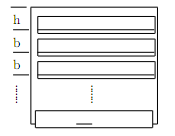
\includegraphics{./graphics/heightofpagebox.jpg}
\end{figure}
\end{comment}

\subsection{Dead cycles.} An execution of the OTR without shipping any material is called a \emph{dead cycle}. Dead cycles, have their uses and we will explain this a bit later on. However, long iterations that just return \textit{dead cycles} is an indication of an error somewhere. \tex counts the number of dead cycles in a counter named |\deadcycles| and stops the run if |\deadcycles >= \maxdeadcycles|.  In the \textit{plain} format |\maxdeadcycles| is set as 25 and in \latex as \the\deadcycles. |\maxdeadcycles = 100| is \the\maxdeadcycles. Each time |\shipout| is invoked, it resets |\deadcycles| to zero.

\begin{dispListing}
If the file is not included, reset \deadcycles, so that a long list of non-included
files does not generate an `Output loop' error.
115 \deadcycles\z@
116 \@nameuse{cp@#1}%
117 \fi
118 \let\@auxout\@mainaux}
\end{dispListing}


\subsection{\tex's Page Number.} The page number can come from any source. Salomon provides an example where the \textsc{OTR} typesets a page number from a |\count| variable. This is typeset centered below the printed area.

%\newpage
%
%Test
%\makeatletter
%
%\let\ltxxoutput\output
%\let\ltxlabel\label@name
%\output={{\let\label@name\@gobble
%  \shipout\vbox{
%  \box255\smallskip
%  \centerline{\thepage}}}
%}
%
%\vfill \penalty-10000
%
%\global\let\output\ltxxoutput
%\let\label@name\ltxlabel
%
%
%\makeatother


Notice that the output macro, just passes the contents of the box to |\shipout|. This is not actually a very good method, but is shown here to illustrate a point.

Note the |\tenrm| in the preceding example. It
is necessary because of the asynchronous nature of
the \otr. When the \otr is invoked, \tex can be
anywhere on the next page. Specifically, it could
be inside a group where a different font is used.
Without the |\tenrm|, that font (the current font)
would be used in the otr.
In the plain format, the |\count0| variable
serves as the page number, and the following two
macros are especially useful.




\subsection{The \texttt{\textbackslash vsplit} operation.} 

Supposed you have inserted the material required to go on a page on a big |\vbox|, but the material is a bit extra that what is required to fill a page exactly. You would need an operation to split the box in two. The |vsplit| operation does that. It is important to the understanding of OTR operations to have an intimate knowledge of |\vsplit|. Its syntax is: 

\begin{quote}
|\vsplit|\meta{box number} to \meta{dim}
\end{quote}

The result of the operation is a box. Most often it appears in an assignment such as: 

\begin{quote}
|\setbox1=\vsplit0 to2.6in| 
\end{quote}

This sets |\box1| to a
height of 2.6in, moves material from the top of
|\box0| to |\box1|, and keeps the remainder in |\box0|.

\begin{macro}{\loremlines}
It is important to remember that most of \tex's commands work with \latex as well. In Example~\ref{ex:loremlines}, we define a box to hold |lipsum| text in a two column layout. We want to define a macro that can split the box in as many lines as we require. 
\end{macro}

\begin{texexample}{Splitting a vbox}{ex:loremlines}
\newbox\one
\newbox\two
\long\gdef\loremlines#1#2{%
   \setbox\one=\vbox {#2}
   \setbox\two=\vsplit\one to #1\baselineskip
   \unvbox\two
   \gdef\boxone{#2}
}
\begin{multicols}{2}
\small
\loremlines{16}{\onepar}
\end{multicols}
\boxone

\setbox\one=\vbox{100}
\the\ht\one \\
\the\baselineskip
\the\splittopskip

\end{texexample}


\tex assumes that the new |\box1| may have to
be shipped out as part of the page. It therefore
places a glue similar to $h$ at the top of |\box1|.
This glue is called \docAuxCommand{splittopskip} and has a plain
format value of 10pt [348].

One important thing to note is that a box can only be split \textit{between} lines of text. 
If we split a box to another size, |\box1| will come out underfull.

Here is an \otr which splits the page, ships
out the top part and returns the rest to the MVL
(actually, to the recent contributions):

\begin{teXXX}
\output={\setbox0=\vsplit255 to1in
\shipout\box0 \unvbox255}
\end{teXXX}






\section{Communicating with the OTR: Marks}


The user can pass information to the output routine through \textit{marks}. Marks have the syntax

\begin{teX}
\mark{mark text}
\end{teX}

which is put in a mark item on the current vertical list. The mark text is subject to expansion
as in \cs{edef}.
If the mark is given in horizontal mode it migrates to the surrounding vertical lists like an
insertion item (see page Text By Topic 77); however, if this is not the external vertical list, the output routine
will not find the mark.

Marks are the main mechanism through which the output routine can obtain information
about the contents of the currently broken-off page, in particular its top and bottom. TEX sets
three variables:

{\obeylines
\cs{botmark} the last mark occurring on the current page;
\cs{firstmark} the first mark occurring on the current page;
\cs{topmark} the last mark of the previous page, that is, the value of \cs{botmark} on the previous
page.
}



If no marks have occurred yet, all three are empty; if no marks occured on the current page, all three variables are equal to the \cs{botmark} of the previous page. 

Marks can be used to get a section heading into the headline or footline of the page.

\begin{quote}
\begin{verbatim}
\def\section#1{ ... \mark{#1} ... }
\def\rightheadline{\hbox to \hsize
    {\headlinefont \botmark\hfil\pagenumber}}
\def\leftheadline{\hbox to \hsize
   {\headlinefont \pagenumber\hfil\firstmark}}
\end{verbatim}
\end{quote}

This places the title of the first section that starts on a left page in the left
headline, and the title of the last section that starts on the right page in
the right headline. Placing the headlines on the page is the job of the output
routine; see below.

It is important that no page breaks can occur in between the mark and the
box that places the title:

\emphasis{mark,nobreak}
\begin{teXXX}
\def\section#1{ ...
   \penalty\beforesectionpenalty
   \mark{#1}
   \hbox{ ... #1 ...}
   \nobreak
   \vskip\aftersectionskip
   \noindent}
\end{teXXX}

%%%%%%%%%%%% macro to put TeX references in right margin %%%%%%%% 
\newdimen\theight 
\def \TeXref#1{% 
             \vadjust{\setbox0=\hbox{\sevenrm\quad\quad\TeX book: #1}% 
             \theight=\ht0 
             \advance\theight by \dp0    \advance\theight by \lineskip 
             \kern -\theight \vbox to \theight{\rightline{\rlap{\box0}}% 
             \vss}% 
             }}% 
%%%%%%%%%%%%%%%%%%%%%%%%%%%%%%%%%%%%%%%%%%%%%%%%%%%%%%%%%%%%%%%%%%%%%%%%% 
 
However, useful these marks, sometimes an output routine (such as those found in \latexe needs to know why it was invoked. Knuth discusses in the \TeXref{396}  another method
that involves the value of the |\outputpenalty|. 
By testing for this value, it is possible to see what penalty occurred at a breakpoint;
any penalty of −10000, −10001, −10002, or less, forces the output routine to
act, hence different penalty values can be used to pass different messages. (When
the output routine puts material back on the list of contributions, it need not restore
the penalty at the breakpoint.) If output has been forced by a highly negative value
of |\outputpenalty|, the output routine can use |\vbox{\unvcopy255}| to discover how
full the page-so-far actually is. Underfull and overfull boxes are not reported when
|\box255| is packaged for use by the output routine, so there’s no harm in ejecting a
page prematurely if you want to pass a signal. (Set |\holdinginserts| positive to pass
a signal when the contents of |\box255| will be sent back through the page builder again,
if any insertions are present.)

Knuth also suggested another method that he called the \emph{dirtiest trick of all} that uses the depth 
of |\box255|. 

\section{Insertions}
Insertions are considered one of  the most  complex  topics in \tex. Many users master  topics  such 
as tokens,  file  I/O, macros,  and  even  OTRS  before they dare  tackle  insertions.  The  reason  is  that 
insertions  are  complex,  and  The \texbook, while 
covering all the relevant material, is somewhat cryptic regarding  insertions, and  lacks  simple examples. 
The  main  discussion  of  insertions takes  place  on 
[115-1251.  where \tex' s  registers  are also discussed. 
Examples  of  insertions are  shown, mostly  without 
explanations,  on  [363-364,  423-424].  A lot of what is described here is based on an article in TUGboat by David Salomon\footnote{\protect\url{http://www.tug.org/TUGboat/Articles/tb11-4/tb30salomon.pdf}}

Many users understand the idea of floats. Certain material to be typeset needs to be held in a buffer and inserted at different points on a page, for example a a figure that does not fit on a page it has to be inserted at the top of the next page. An \textit{insertion} is just a piece of a document that is generated at a certain point but appears at another point. Common examples are figures, footnotes and endnotes. Quoting Knuth:

\begin{quote}
  This  algorithm  is  admittedly  complicated, 
but  no  simpler  mechanism  seems  to  do  nearly 
as  much.
\end{quote}

\section{\protect\textbackslash shipout}

The primitive control sequence \docAuxCommand{shipout} is \tex's end game. It's syntax is quite simple:

\begin{quote}
|\shipout<box>|
\end{quote}

From TeXbook, Chapter 23: Output Routines, page 254:

\begin{quotation}
TeX’s primitive command |\shipout<box>| is what actually causes output. It sends the contents of the box to the dvi file, which is TeX’s main output file; after TeX has finished, the dvi file will contain a compact device-independent encoding of instructions that specify exactly what should be printed. When a box is shipped out, TeX displays the values of |\count0| through |\count9| on your terminal, as explained in Chapter 15; these ten counters are also recorded in the dvi file, where they can be used to identify the page. All of the |\openout, \closeout|, and |\write| commands that appear inside of the box are performed in their natural order as that box is being shipped out. Since a |\write| command expands macros, as explained in Chapter 21, TeX’s scanning mechanism might detect syntax errors while a |\shipout| is in progress. If  |\tracingoutput| is nonzero at the time of a \cs{shipout}, the contents of the box being shipped are written into your log file in symbolic form. You can say \cs{shipout} anywhere, not only in an output routine.
\end{quotation}


We can say:

\emphasize{shipout,vbox}
\begin{teXXX}
\shipout\vbox{%
  \hrule
  \medskip
  \lipsum[1-5]
  \medskip
  
  This is a Test for shipout
  
  \hrule
}
\end{teXXX}

\shipout\vbox{%
  \hrule
  \medskip
  \lipsum[1-5]
  \medskip
  \centering
  \textbf{Sample: }{This is a Test for shipout}
  \hrule
}

Since the output box handled by \tex still holds material the page is shown in the previous page. There is no page numbers or headers and it just shows he lorem-ipsum text and a primitive caption at the bottom. I have written the example to show the difference between the logical and actual pages. TeX does not care how the page will look, it will assemble it put headers, page numbers and pass it on to shipout. Shipout will then insert it to the dvi file, which will hold all teh instructions to print a real page.

We can modify the example to add our head and foot. 

\begin{texcode}{Shipout}{ex:ship2}
This will print by the normal routine

\long\gdef\boxit#1#2{\hbox{\vrule \vbox{\hrule\kern#2pt\hbox{%
\kern#2pt\vbox{#1}\kern#2pt}\kern#2pt\hrule}\vrule}}

\makeatletter
\shipout\vbox {%
  \vskip\topsep\relax
  \vskip\headsep
   \@thehead
   \vskip30pt
    \boxit{
      \lipsum[1-5]
      }{2}
   \vskip30pt
   \@thefoot   
}
\makeatother 
\end{texcode}

\latexe's output routine takes care of all the page geometry, the details to set up the headers and footers, but most importantly intercepts teh contents of the output box measure it, cuts it inserts the inserts such as footnotes and figures, margin notes, separates the text in two columns if necessary and so on. 

\long\gdef\boxit#1#2{\hbox{\vrule \vbox{\hrule\kern#2pt\hbox{%
\kern#2pt\vbox{#1}\kern#2pt}\kern#2pt\hrule}\vrule}}
\makeatletter
\shipout\vbox {%
  \vskip\topsep\relax
  \vskip\headsep
   \@thehead
   \vskip30pt
    \boxit{
      \lipsum[1-5]
      }{2}
   \vskip30pt
   \@thefoot   
}
\makeatother 



An output routine will prepare the virtual page and pass it onto a 

Here is an OTR for a \textit{framed} page. It surrounds the
page with double rules on all sides, and centers the
page number below the double box. Note that the
page shipped out is wider and taller than \cs{box255}.
The value of \cs{hsize} in this case is, therefore, not
the width of the final page shipped out, but the
width of the text lines in \cs{box255}.

Macro \cs{frameit} typesets text and surrounds it
with 4 rules (see [Ex. 21.3]). Parameter \#2 is the
space between the rules and the text. \#1 is a box
containing the text.

\emphasis{output,shipout}
\begin{texcode}{Example of simple output routine}{ex:output1}
\def\frameit#1#2{%
 \vbox{\hrule
  \hbox{%
    \vrule \kern#2pt
      \vbox{\kern#2pt #1
         \kern#2pt}%
      \kern#2pt\vrule}
\hrule}}

\output={
   \shipout\vbox{
   \boxit{\frameit{\box255}9}
      \medskip
      \centerline{Test Framed Page}}
  \advancepageno}
\end{texcode}

 

So far we did not care if the height of the page is right or not. In production code the shipout holds
a box, which has been produced by \tex. Any material we add to it, must not affect the dimensions of the box.
If we do and is too big the drivers will probably clip it.


Plain TeX has an output routine that takes care of  simple things like page numbering and insertions
using \cs{footnote} and \cs{topinsert}. 


So far we have examined the \tex OTR in detail. I hope it has given you enough understanding, not only to write your own output routine, but also to now be ready to study the \latex output routine, which is much more complicated. We have so far seen that  when \tex 
is typesetting pages of continuous text, it will gather material until it can find a least-cost page break intended to
make the gathered material fit the \cs{pagegoal} size. The
gathered material will then be placed into |\box255| and
the output routine stored in the token register \cs{output}
will be processed in a group of its own. 

Usually it will
arrange the gathered material in some way, add headers,
footlines and page numbers, and ship the gathered results out in typeset form with the \cs{shipout} command.
At the time of the \cs{shipout} command all \cs{open} and
\cs{write} commands stored in the box shipped out are expanded and written out. This is what makes it possible to have page labels corresponding to the actual page
numbers at the time of shipout: the corresponding info
is written to the |.aux| file at that time.
The output routine may decide to place material
back on the main vertical list instead of shipping it out. Its ob is to check if it can have a break, if it can it will ship the page out. If it cannot it will palce the material back on the main vertical list. 

\section{\LaTeX\  output routines}


\LaTeX\ output routine is described in \texttt{ltoutput.dtx}. You should also have a look at \texttt{ltfloat.dtx}. The algorithm is revisited i \latex3 and Frank Mittelbach, published a paper
\footnote{\protect\url{http://www.latex-project.org/papers/xo-pfloat.pdf}} in which he explains some of the problems facing the team, when dealing with the output routine.


Information on the output routine is rather scarce. Best source is a series of  articles in the TUGBoat by David Salomon.

\href{http://www.tug.org/TUGboat/Articles/tb11-1/tb27salomon.pdf}{Output Routines: Examples and Techniques. Part I: Introduction and Examples.}

\href{http://www.tug.org/TUGboat/Articles/tb11-2/tb28salomon.pdf}{Output Routines: Examples and Techniques. Part II: OTR Techniques}

\href{http://www.tug.org/TUGboat/Articles/tb11-4/tb30salomon.pdf}{Output Routines: Examples and Techniques. 
Part III: Insertions}

\href{http://www.tug.org/TUGboat/Articles/tb15-1/tb42salomon-output.pdf}{Output routines: Examples and techniques Part IV: Horizontal techniques}


David Kastrup's article \href{http://www.tug.org/TUGboat/Articles/tb24-3/kastrup.pdf}{Output Routine Requirements for Advanced Typesetting Tasks} (Proceedings of EuroTEX 2003) otlined some of the difficult areas and specifications for generic routines

The standard blocks are well described above and most tasks could be accomplished 
by rather working from
standard building blocks like \textit{insertion lists}, \textit{here points},
default mechanisms for \textit{margin notes} and so on.


%\section{Calling the output routine}
%
%The output routine is called either by TeX's normal page-breaking
%mechanism, or by a macro putting a penalty < or = -10000 in the output
%list. In the latter case, the penalty indicates why the output
%routine was called, using the following code.
%penalty reason
%
%\begin{longtable}{ll}
%\toprule
%penalty &reason\\
%\midrule
%-10000  &\ pagebreak\\
%~       &\ newpage\\
%-10001  &clearpage (\ penalty -10000 \ vbox{}| \ penalty -10001)|\\
%-10002  &float insertion, called from horizontal mode\\
%-10003 &float insertion, called from vertical mode.\\
%-10004 &float insertion.\\
%\bottomrule
%\end{longtable}
%\medskip
%
%Note: A |float| or |marginpar| puts the following sequence in the output
%list: 
%
%\begin{enumerate}
%\item a penalty of -10004,
%
%\item a null |\vbox|
%
%\item a penalty of -10002 or -10003.
%\end{enumerate}
%
%This solves two special problems:
%
%\begin{enumerate}
%\item If the float comes right after a |\newpage| or |\clearpage|,
%then the first penalty is ignored, but the second one
%invokes the output routine.
%
%\item If there is a split footnote on the page, the second 'page'
%puts out the rest of the footnote
%\end{enumerate}
%
%\latex first defines some helper routines and increase the \cs{maxdeadcycles}. The helper macros are for
%manipulating lisst.
%
%\begin{teX}
% \maxdeadcycles = 100
% \let\@elt\relax
% \def\@next#1#2#3#4{\ifx#2\@empty #4\else
%   \expandafter\@xnext #2\@@#1#2#3\fi}
%   \@next \CS \LIST {NONEMPTY}{EMPTY} == %% NOTE: ASSUME
%\@elt = \relax
% BEGIN assume that \LIST == \@elt \B1 ... \@elt \Bn
% if n = 0
% then EMPTY
% else 
%   \CS :=L \B1
%   \LIST :=G \@elt \B2 ... \@elt \Bn
%   NONEMPTY
% fi
%END
%\end{teX}
%
%
%\begin{teX}
%11 \def\@xnext \@elt #1#2\@@#3#4{\def#3{#1}\gdef#4{#2}}
%
%12 \def\@testfalse{\global\let\if@test\iffalse}
%13 \def\@testtrue {\global\let\if@test\iftrue}
%14 \@testfalse}
%   }
%
%15 \def\@bitor#1#2{\@testfalse {\let\@elt\@xbitor
%16   \@tempcnta #1\relax #2}}
%
%17 \def\@xbitor #1{\@tempcntb \count#1
%18    \ifnum \@tempcnta =\z@
%19    \else
%20      \divide\@tempcntb\@tempcnta
%21    \ifodd\@tempcntb \@testtrue\fi
%22   \fi}
%\end{teX}
%
%
%\subsection{Float boxes and lists.} 
%A \textit{float list} consisting of the 
%floats in boxes |\boxa ... \boxN| has
%the form:
%
%|\@elt \boxa ... \@elt \boxN|
%where |\boxI| is defined by
%
%|\newinsert\boxI|
%
%Normally, |\@elt| is |\let| to |\relax|. A test can be performed on the
%entire 
%oat list by locally |\def|'ing |\@elt| appropriately and
%executing the list.
%This is a lot more efficient than looping through the list.
%\LaTeX\ defines float boxes as |bx@A| to |bx@R| to make them available for 
%inserts. These will be used later to define the lists that hold these boxes. 
%
%\latex now defines the float boxes. Each one is defined as an \cmd{\newinsert.}
%
%\begin{teXXX}
%\newinsert\bx@A
%...
%\newinsert\bx@I
%\newinsert\bx@J
%\newinsert\bx@K
%\newinsert\bx@L
%\newinsert\bx@M
%\newinsert\bx@N
%\newinsert\bx@O
%\newinsert\bx@P
%\newinsert\bx@Q
%\newinsert\bx@R
%\end{teXXX}
%
%
%
%Once these boxes are defined they are inserted in the |@freelist|. At this point all the other lists are defined.
%
%\emphasis{@freelist,@toplist,@botlist,@midlist,@currlist}
%\begin{teXXX}
%41 \gdef\@freelist{\@elt\bx@A\@elt\bx@B\@elt\bx@C\@elt\bx@D
%         \@elt\bx@E
%42                 \@elt\bx@F\@elt\bx@G\@elt\bx@H\@elt\bx@I\@elt\bx@J
%43                 \@elt\bx@K\@elt\bx@L\@elt\bx@M\@elt\bx@N
%44                 \@elt\bx@O\@elt\bx@P\@elt\bx@Q\@elt\bx@R}
%\end{teXXX}
%
%\startlineat{45}
%All the lists are defined initially to be empty.
%\begin{teXXX}
%45 \gdef\@toplist{}
%46 \gdef\@botlist{}
%47 \gdef\@midlist{}
%48 \gdef\@currlist{}
%49 \gdef\@deferlist{}
%50 \gdef\@dbltoplist{}
%51 \gdef\@dbldeferlist{}
%\end{teXXX}
%
%
%The lists are similar to those defined in \texttt{plain}.
%
%\begin{description}
%\item[\cs{@freelist}] : List of empty boxes for placing new 
%floats.
%\item[\string\@toplist] : List of 
%floats to go at top of current column.
%\item[\string\@midlist] : List of 
%floats in middle of current column.
%\item[\string\@botlist] : List of 
%floats to go at bottom of current column.
%\item[\string\@deferlist] : List of 
%floats to go after current column.
%\item[\string\@dbltoplist] : List of double-col. 
%floats to go at top of current
%page.
%\item[\string\@dbldeferlist] : List of double-column 
%floats to go on subsequent
%pages.
%
%\end{description}
%
%\begin{multicols}{2}
%Check was prudent when defining the newinsert boxes in order to reserve space and memory. The package \docpkg{morefloats} can be used to add more floats to this list. This should have definitely been included here in a revision.
%
%\subsection{Defining Layout parameters} All the page layout parameters are defined next. 
%
%\begin{teXXX}
%52 \newdimen\topmargin
%53 \newdimen\oddsidemargin
%54 \newdimen\evensidemargin
%55 \let\@themargin=\oddsidemargin
%56 \newdimen\headheight
%57 \newdimen\headsep
%58 \newdimen\footskip
%59 \newdimen\textheight
%60 \newdimen\textwidth
%61 \newdimen\columnwidth
%62 \newdimen\columnsep
%63 \newdimen\columnseprule
%64 \newdimen\marginparwidth
%65 \newdimen\marginparsep
%66 \newdimen\marginparpush
%\end{teXXX}
%
%Remember  that TeX knows little about a page. The problem is that TEX has no idea how
%wide and tall the paper is. All it knows is the
%left and top offsets, and the dimensions of the
%printed area (|\hsize| and |\vsize|). All these dimensions need to be calculated and adjustments made within the \otr.
%
%A document normally  starts by specifying:
%
%\begin{teXXX}
%\newdimen\paperheight
%\newdimen\paperwidth
%\paperheight=..in \paperwidth=..in
%\end{teXXX}
%
%
%\end{multicols}
%
%
%\subsection*{The AtBeginDvi}
%A box register is used  to put stuff that must appear before anything else
%in the |.dvi| file.
%
%The stuff in the box should not add any typeset material to the page when it
%is unboxed.
%
%\emphasis{AtBeginDvi,@begindvibox}
%
%\begin{teXXX}
%67 \newbox\@begindvibox
%68 \def \AtBeginDvi #1{%
%69 \global \setbox \@begindvibox
%70 \vbox{\unvbox \@begindvibox #1}%
%71 }
%\end{teXXX}
%
%\begin{teXXX}
%72 \newdimen\@maxdepth
%73 \@maxdepth = \maxdepth
%\end{teXXX}
%
%
%Some new registers for paperheight and paperwidth are defined:
%
%\begin{teXXX}
%74 \newdimen\paperheight
%75 \newdimen\paperwidth
%76 \newif \if@insert
%These should definitely be global:
%77 \newif \if@fcolmade
%78 \newif \if@specialpage \@specialpagefalse
%These should be global but are not always set globally in other les.
%79 \newif \if@firstcolumn \@firstcolumntrue
%80 \newif \if@twocolumn \@twocolumnfalse
%Not sure about these: two questions. Should things which must apply to a whole
%doument be local or global (they probably should be `preamble only' commands)?
%Are these three such things?
%81 \newif \if@twoside \@twosidefalse
%82 \newif \if@reversemargin \@reversemarginfalse
%83 \newif \if@mparswitch \@mparswitchfalse
%This counter has been imported from `multicol'.
%84 \newcount \col@number
%85 \col@number \@ne
%\end{teXXX}
%
%and a lot of other internal registers
%
%\begin{teX}
%86 \newcount\@topnum
%87 \newdimen\@toproom
%88 \newcount\@dbltopnum
%89 \newdimen\@dbltoproom
%90 \newcount\@botnum
%91 \newdimen\@botroom
%92 \newcount\@colnum
%93 \newdimen\@textmin
%94 \newdimen\@fpmin
%95 \newdimen\@colht
%96 \newdimen\@colroom
%97 \newdimen\@pageht
%98 \newdimen\@pagedp
%99 \newdimen\@mparbottom \@mparbottom\z@
%100 \newcount\@currtype
%101 \newbox\@outputbox
%102 \newbox\@leftcolumn
%103 \newbox\@holdpg
%104 \def\@thehead{\@oddhead} % initialization
%105 \def\@thefoot{\@oddfoot}
%\end{teX}
%
%
%\subsection{\texttt{\textbackslash clearpage}}
%
%\begin{macro}{\clearpage}
%The clearpage macro is a bit complicated, as it needs to avoid a complete empty page after a |\twocolumn[..]|. This prevents the text from the argument
%vanishing into a  float box, never to be seen again. We hope that it does not
%produce wrong formatting in other cases.
%\end{macro}
%
%\begin{teXXX}
%106 \def\clearpage{%
%107   \ifvmode
%108   \ifnum \@dbltopnum =\m@ne
%109     \ifdim \pagetotal <\topskip
%110       \hbox{}%
%111     \fi
%112   \fi
%113  \fi
%114 \newpage
%115 \write\m@ne{}%
%116 \vbox{}%
%117 \penalty -\@Mi
%118 }
%\end{teXXX}
%
%\subsection{The \texttt{\textbackslash clearpagedoublepage} macro} 
%
%\begin{macro}{cleardoublepage}
%This checks for odd and even pages by using the
%page counter |c@page|.  It also provides switches of twoside printing. 
%
%\numberlineat{119}
%\begin{teXXX}
%\def\cleardoublepage{%
%   \clearpage
%   \if@twoside 
%     \ifodd\c@page
%     \else
%       \hbox{}
%       \newpage
%       \if@twocolumn\hbox{}\newpage
%       \fi
%     \fi
%  \fi}
%\end{teXXX}
%\end{macro}
%
%Note the |\newpage| is defined a bit further on. This is a fairly simple definition, since most of the code that follows only gets a bit complicated with the twocolumn option. It sets the dimensions and the booleans to those appropriate for the |onecolumn| option. An important note we back to \tex's |\hsize|. Both the linewidth as well as the columnwidth are set to this.
%
%\begin{teXXX}
%123 \def\onecolumn{%
%124   \clearpage
%125   \global\columnwidth\textwidth
%126   \global\hsize\columnwidth
%127   \global\linewidth\columnwidth
%128   \global\@twocolumnfalse
%129   \col@number \@ne
%130   \@floatplacement
%     }
%\end{teXXX}
%
%\subsection{\string newpage.} 
%
%The |\newpage| macro is programmed defensively. The two checks at the beginning ensure that an item label or run-in section title
%immediately before a |\newpage| get printed on the correct page, the one before
%the page break.
%All three tests are largely to make error processing more robust; that is why
%they all reset the 
%flags explicitly, even when it would appear that this would be
%done by a |\leavevmode|.
%
%\begin{teXXX}
%131 \def \newpage {%
%132  \if@noskipsec
%133    \ifx \@nodocument\relax
%134      \leavevmode
%135      \global \@noskipsecfalse
%136    \fi
%137 \fi
%138 \if@inlabel
%139   \leavevmode
%140   \global \@inlabelfalse
%141 \fi
%142 \if@nobreak \@nobreakfalse \everypar{}\fi
%143 \par
%144 \vfil
%145 \penalty -\@M}
%\end{teXXX}
%
%An empty cols is defined. There is a note here, that an invisible rule might have been a better idea.
%
%\begin{teXXX}
%146 \def \@emptycol {\vbox{}\penalty -\@M}
%\end{teXXX}
%
%\subsection{The \string twocolumn macro.} This is the longest definition so far. We will leave it for a while and then come back. There are several bug fixes to the two-column stuff here. Firstly, like the onecolumn the page parameters are set to the correct parameters.
%
%
%\begin{teXXX}
%147 \def \twocolumn {%
%148 \clearpage
%149 \global\columnwidth\textwidth
%150 \global\advance\columnwidth-\columnsep
%151 \global\divide\columnwidth\tw@
%152 \global\hsize\columnwidth
%153 \global\linewidth\columnwidth
%154 \global\@twocolumntrue
%155 \global\@firstcolumntrue
%156 \col@number \tw@
%\end{teXXX}
%
%
%
%\section{The output macro}
%
%The setting of the \cs{output} is quite short but it belies its complexity.
%After having checked verious parameters it redirects to |@specialoutput|. This is the heart of the routines. Notice that \latex just fills in the token list of \tex's |output| routine, it does not attempt to redefine it or save it. 
%Should some hooks be defined here, life might have been made easier, however, what one can do is to first save the \latex output routine and then redefine the output as one may wish. Return to it can happen after it. If you take this approach, you should be careful of packages that redefine output, such as |multicol| and |longtable|. An approach such as this is taken by \citeauthor{revtex} in the \pkgname{revtex} class.\footcite[][This is a document class of the American Physical Society. It enables submission to any of the APS journals. Its distribution point is \protect\url{http://publish.aps.org/revtex4/}]{revtex}
%
%\emphasis{ifnum,fi,else,ifdimen,@specialoutput}
%\begin{teX}
%204 \output {%
%205 \let \par \@@par
%206 \ifnum \outputpenalty<-\@M
%207    \@specialoutput
%208 \else
%209    \@makecol
%210    \@opcol
%211    \@startcolumn
%212    \@whilesw \if@fcolmade \fi
%213      {%
%218      \@opcol\@startcolumn}%
%219 \fi
%220 \ifnum \outputpenalty>-\@Miv
%221 \ifdim \@colroom<1.5\baselineskip
%222 \ifdim \@colroom<\textheight
%223 \@latex@warning@no@line {Text page \thepage\space
%224 contains only floats}%
%225 \@emptycol
%226 % \if@twocolumn
%227 % \if@firstcolumn
%228 % \else
%229 % \@emptycol
%230 % \fi
%231 % \fi
%232 \else
%  233 \global \vsize \@colroom
%234 \fi
%235 \else
%236   \global \vsize \@colroom
%237 \fi
%238 \else
%239   \global \vsize \maxdimen
%240 \fi
%241 }
%\end{teX}
%
%
%
%\begin{teXXX}
%244 \gdef\@specialoutput{%
%245   \ifnum \outputpenalty>-\@Mii
%246     \@doclearpage
%247   \else
%248     \ifnum \outputpenalty<-\@Miii
%249         \ifnum \outputpenalty<-\@MM \deadcycles \z@ \fi
%250                 \global \setbox\@holdpg \vbox {\unvbox\@cclv}%
%251         \else
%252         \global \setbox\@holdpg \vbox{%
%253                 \unvbox\@holdpg
%254                 \unvbox\@cclv
%We must now remove the box added by the 
%oat mechanism and the \topskip
%glue therefore added above it by TEX.
%255                \setbox\@tempboxa \lastbox
%256                \unskip
%257 }%
%These two are needed as separate dimensions only by \@addmarginpar; for other
%purposes we put the whole size into \@pageht (see below).
%258                \@pagedp \dp\@holdpg
%259                \@pageht \ht\@holdpg
%260                \unvbox \@holdpg
%
%261                \@next\@currbox\@currlist{%
%262                \ifnum \count\@currbox>\z@
%Putting the whole size into \@pageht (see above).
%263                  \advance \@pageht \@pagedp
%264                  \ifvoid\footins \else
%265                    \advance \@pageht \ht\footins
%266                    \advance \@pageht \skip\footins
%267                    \advance \@pageht \dp\footins
%268                \fi
%\end{teXXX}
%
%
%
%\subsection{The \string @doclearpage macro.} This is an emergency action. It dumps everything: footnotes first and then floats. 
%
%
%\section*{The Kludgeins}
%
%The kludgeins are simply inserts that fool \tex in enlarging a page by a small amount, normally used to allow one or two lines of text to go in the same page.
%
%The two kludgeins mentioned in the kernel are are \cs{enlargethisspace} and its star version.\footnote{The Oxford English Dictionary (2nd ed., 1989) kludge entry cites one source for this word's earliest recorded usage, definition, and etymology: Jackson W. Granholm's 1962 "How to Design a Kludge" article, which appeared in the American computer magazine Datamation
%kludge  Also kluge. [J. W. Granholm's jocular invention: see first quot.; cf. also bodge v., fudge v.]
%
%'An ill-assorted collection of poorly-matching parts, forming a distressing whole' (Granholm); esp. in Computing, a machine, system, or program that has been improvised or 'bodged' together; a hastily improvised and poorly thought-out solution to a fault or 'bug'.
%
%The word 'kludge' is...derived from the same root as the German Kluge..., originally meaning 'smart' or 'witty'.... 'Kludge' eventually came to mean 'not so smart' or 'pretty ridiculous'.}
%
%
%
%\begin{teXX}
%\gdef \enlargethispage{%
%1198 \@ifstar
%1199 {%
%1203   \@enlargepage{\hbox{\kern\p@}}}%
%1204 {%
%1208   \@enlargepage\@empty}%
%1209 }
%\end{teXX}
%
%Adds |<dim>| to the height of the current column only. On the printed page the
%bottom of this column is extended downwards by exactly |<dim>| without having
%any effect on the placement of the footer; this may result in an overprinting.
%\cs{enlargethispage}.
%
%Similar to |\enlargethispage| but it tries to squeeze the column to be printed
%in as small a space as possible, ie it uses any shrinkability in the column. If the
%column was not explicitly broken (e.g. with |\pagebreak|) this may result in an
%overfull box message but except for this it will come out as expected (if you know
%what to expect).
%The star form of this command is dedicated to Leslie Lamport, the other we
%need for ourselves (FMi, CAR).
%These commands may well have unwanted if used soon before a\ldots
%
% 




\section{Packages}

OTR routines are notoriously difficult to debug and define. Some of the available packages at CTAN
can make the programming job easier.

The \pkg{everypage} package by Sergio Callegari provides hooks into the \latex\ internal commands to
to do actions on every page or on the current page. Specifically, actions  are performed \emph{before} the page is shipped, so they can be used to put watermarks \emph{in the background} of a page, or to
set the page layout. 

The package provides two hooks:

\emphasis{AddEverypageHook,AddThisPageHook}
\begin{teXXX}
  \AddEverypageHook{Test}
  \AddThisPageHook
\end{teXXX}

The package reminds in some sense
\pkgname{bobhook} by Karsten Tinnefeld, but it differs in the way in
 which the hooks are implemented, as detailed in the following.
 In some sense it may also be related to the package
 \pkgname{everyshi} by Martin Schroeder, but again the implementation
 is different.

 
 This program adds two \LaTeX\ hooks that get run when document
 pages are finalized and output to the |.dvi| or |.pdf|
 file. Specifically, one hook gets executed on every page, while the
 other is executed for the current page. Hook actions are are performed
 \emph{before} the page is output on the medium, and this is
 important to be able to play with the page layout or to put things
 \emph{behind} the page contents (e.g., watermarks such as an image,
 framing, the ``DRAFT'' word, and the like).
 
 The package reminds in some sense \pkg{bobhook} by Karsten
 Tinnefeld, but it differs in the way in which the hooks are
 implemented:
 


 \begin{enumerate}
 \item there is no formatting inherent in the hooks. If one wants to
   put some watermark on a page, it is his own duty to put in the
   hook the code to place the watermark in the right position. Also
   note that the hooks code should \emph{eat up no space} in the
   page.  Again, if the hooks are meant to place some material on the
   page, it is the duty of the hook programmer to put code in the
   hooks to pretend that the material has zero width and zero height.
   The implementation is \emph{lighter} than the \Lpack{bobhook} one,
   and possibly more flexible, since one is not limited by any
   pre-coded formatting for the hooks. On the other hand it is
   possibly more difficult to use. Nonetheless, it is easy to think
   of other packages relying on \Lpack{everypage} to deliver more
   user-friendly and \emph{task specific} interfaces. Already there
   are a couple of them: the package \Lpack{flippdf} produces
   mirrored pages in a PDF document and \Lpack{draftwatermark}
   watermarks document pages.
 \item similarly to \Lpack{bobhook} and \Lpack{watermark}, the
   package relies on the manipolatoin of the internal \LaTeX\ macro
   |\@begindvi| to do the job. However, the redefinition of
   |\@begindvi| is here postponed as much as possible, striving to
   avoid interference with other packages using |\AtBeginDvi| or
   anyway manipulating |\@begindvi|. Specifically \Lpack{everypage}
   makes no special assumption on the initial code that |\@begindvi|
   might contain.
 \end{enumerate}



Also in some sense \pkgname{everypage} can be related to package
 \pkgname{everyshi} by Martin Schr\"oeder \cite{everyshi}, but it differs radically from
 it in the implementation. In fact,\pkgname{everypage} operates by
 manipulation of the |\@begindvi| macro, rather than at the
 lower level |\shipout| macro.

\section{hooking at shipout}

\begin{docCmd} {EveryShipout} {}
\begin{docCmd} {AtNextShipout} {}
This package provides the hooks \cs{EveryShipout} and 
  \cs{AtNextShipout} whose arguments are executed after the output 
  routine has constructed \cs{box255}, and before \cs{shipout} is 
  called.
\end{docCmd}
\end{docCmd}

An example application for this package would be a package for
 adding text to the bottom of each page.
 The  \pkgname{prelim2e} package adopts this method \citep{prelim2e}.\footcite{prelim2e}

The solution  uses is based on code developed in  |quire.tex| by
 Marcel R.~van der Goot.\footcite{quire}  

The \pkgname{prelim2e}  intercepts and modifies the |\box255|. 

\begin{teX}
44 \newcommand{\@Prelim@EveryShipout}{%
45 \bgroup
% First we save the dimensions of \box255: height, width and depth; and calculate
% the total height of \box255.
46 \dimen\z@=\wd\@cclv
47 \dimen\@ne=\ht\@cclv
48 \dimen\tw@=\dp\@cclv
49 \dimen\thr@@=\dimen1
50 \advance\dimen\thr@@ by \dimen\tw@
% Then we set \box255: A \vbox to the total height of \box255. In this a \hbox to
% the width of \box255 is included, in which \box255 is set.
51 \global\setbox\@cclv\vbox to \dimen\thr@@{%
52 \hb@xt@\dimen\z@{%
53 \box\@cclv%
54 \hss
55 }%
\end{teX}
To this we append the text produced by |\PrelimText|. It is put in a |\vbox to 0pt|
in which a |\hbox| to the width of |\box255| is included, in which |\PrelimText| is set.
We have to reset |\protect| because it is set to |\noexpand| by the output routine.

\begin{teXXX}
56 \vbox to \z@{%
57   \hb@xt@\dimen\z@{%
58     \let\protect\relax
59     \hfill\PrelimText\hfill
60   }%
61   \vss
62 }%
63   \vss
64 }%
\end{teXXX}

Finally we set the dimensions of |\box255| to the values they had before |\@Prelim@EveryShipout|.

\begin{teX}
65 \wd\@cclv=\dimen\z@
66 \ht\@cclv=\dimen\@ne
67 \dp\@cclv=\dimen\tw@
68 \egroup
69}
\end{teX}

Once the command is defined, it is hooked into the system via |\EveryShipout| when it is in draft mode. 

\begin{teX}
70 \if@prelim@draft
71 \EveryShipout{\@Prelim@EveryShipout}
72 \fi
\end{teX}

\section{How to place a background image}

One can use \tikzname to place a background image or some text on a page

First we define some utility macros:


\begin{teX}
\def\bg@contents{Draft}
\def\bg@color{red!45}
\def\bg@angle{60}
\def\bg@opacity{.5}
\def\bg@scale{15}
\def\bg@position{current page.center}
\def\bg@anchor{}
\def\bg@hshift{0}
\def\bg@vshift{0}
\end{teX}

A new command is then developed to describe the background material

\begin{teXXX}
\newcommand\bg@material{%
   \begin{tikzpicture}[remember picture,overlay]
   \node [rotate=\bg@angle,scale=\bg@scale,opacity=\bg@opacity,%
   xshift=\bg@hshift,yshift=\bg@vshift,color=\bg@color]
   at (\bg@position) [\bg@anchor] {\bg@contents};
  \end{tikzpicture}}%
\end{teXXX}


Once the background material has been defined we can place it on the page by simply calling:

\begin{teX}
\newcommand\BgThispage{\AddThispageHook{\bg@material}}
\end{teX}


The \pkgname{background}\footcite{background} package by \citeauthor has capitalized on two good packages the \tikzname and the \pkgname{everypage}.
\footcite{everypage} As most of modern
\tex programming works with |pdf| files, package developers prefer to use \tikzname methods for hooking directly into the pdf and thus avoid a trip into the output routine. If it is required then it hooks via the dvi or shipout commands.\footnote{These packages are loaded automatically by the \pkgname{phd-pkgmanager}.}



\vfill

\message{(total: \the\pagetotal
depth: \the\pagedepth
shrink: \the\pageshrink
stretch: \the\pagestretch}



 







































% 
%</driver>
% \fi
% 
%  \CheckSum{0}
%  \CharacterTable
%  {Upper-case    \A\B\C\D\E\F\G\H\I\J\K\L\M\N\O\P\Q\R\S\T\U\V\W\X\Y\Z
%   Lower-case    \a\b\c\d\e\f\g\h\i\j\k\l\m\n\o\p\q\r\s\t\u\v\w\x\y\z
%   Digits        \0\1\2\3\4\5\6\7\8\9
%   Exclamation   \!     Double quote  \"     Hash (number) \#
%   Dollar        \$     Percent       \%     Ampersand     \&
%   Acute accent  \'     Left paren    \(     Right paren   \)
%   Asterisk      \*     Plus          \+     Comma         \,
%   Minus         \-     Point         \.     Solidus       \/
%   Colon         \:     Semicolon     \;     Less than     \<
%   Equals        \=     Greater than  \>     Question mark \?
%   Commercial at \@     Left bracket  \[     Backslash     \\
%   Right bracket \]     Circumflex    \^     Underscore    \_
%   Grave accent  \`     Left brace    \{     Vertical bar  \|
%   Right brace   \}     Tilde         \~}
%
%
%
% \changes{1.0}{2018/01/26}{Converted to DTX file}
%
% \DoNotIndex{\newcommand,\newenvironment}
% \GetFileInfo{phd.dtx}
% 
%  \def\fileversion{v1.0}          
%  \def\filedate{2012/03/06}
% \title{The \textsf{phd} package.
% \thanks{This
%        file (\texttt{phd-utils.dtx}) has version number \fileversion, last revised
%        \filedate.}
% }
% \author{Dr. Yiannis Lazarides \\ \url{yannislaz@gmail.com}}
% \date{\filedate}
% 
% ^^A\maketitle
% 
% ^^A\frontmatter
%  ^^A\coverpage{./images/hine02.jpg}{Book Design }{Camel Press}
% ^^A\secondpage
% \pagestyle{empty}
%  \begin{abstract}
%   This is the Ukrainian language module for the {datetime2}
%   package. If you want to use the settings in this module you must
%   install it in addition to installing \pkg{datetime2}. If you use
%   {babel} or {polyglossia}, you will need this module to
%   prevent them from redefining \cs{today}. The {datetime2}
%   {useregional} setting must be set to "text" or "numeric"
%   for the language styles to be set.
%   Alternatively, you can set the style in the document using
%   \cs{DTMsetstyle}, but this may be changed by \cs{dateukrainian}
%   depending on the value of the {useregional} setting.
% \end{abstract}
% 
% \chapter{The phd-i18n Package}
% One of the primary aims of the package was to simplify the user interface. At the 
% author level, if one has the appropriate stylesheet, nothing needs to be done.
%
% \section{Usage}
%
% To set the main language of the document use:
%  \begin{sverbatim}
%    \cxset{locale german}
%  \end{sverbatim}
%
% This is best done early in the preamble.
%
% To use any secondary language in the text, there is no need with LuaLaTeX to 
% do anything in the preamble. Just use the appropriate |\text| command.
%   \begin{quote}
%     |\textgerman{your text here}|
%   \end{quote}
%
% For longer texts you can use the environment type commands:
%   \begin{quote}
%     |\begin{ngerman}|\\
%     |\end{ngerman}|
%   \end{quote}
%
% All locale names can be inputted in multiple ways: a) Using thelowercase name of the language as found
% in polyglossia or Babel. Using a title case of the language name i.e., |Greek| or |greek|. You can also use 
% the ISO two code or BCF47 codes for greek it would be |el|. If there are dialects you can use |UKenglish|, as in Babel. Remember you only input the main language. If you do not and the package is included it will default
% to |UKenglish|. 
%
% ^^A \StopEventually{}
%  \OnlyDescription
%
%  ^^A\StopEventually{\printindex}
% \vfill
%<*package>
% \CodelineNumbered
% \pagestyle{headings}
% \def\chaptername{\appendixname}
% \appendix
% \chapter{Implementation}
%
% \section{Specification}
%
% \begin{enumerate}
%  \item  Provide translation strings for all languages listed in
%     the Babel and polyglossia packages and extend this to all the unicode languages.
%  \item  Handle date time.
%  \item Provide useful macros.
%  \item Set quotation marks for the language.
%  \item Provide lua code where appropriate.
%  \item Handle specific numerals, for languages that have their own
%        numerals.
%  \item Handle text directionality without having to load the bidi package.
%  \item Handle Asian languages.
%  \item Rationalize methodology and algorithms as far as possible.
%  \item Enable traditional typesetting rules for the language. I am not too sure if this
%        belongs here, as at least for sectioning commands this is provided by the sectioning
%        keys, however it makes no harm to re-intoduce it here.
%        \begin{enumerate}
%          \item Different enumerate environments (e.g. for French).
%          \item Indentation of paragraphs after sections (e.g. French, basque, Ukrainian).
%          \item French spacing after punctuation.
%          \item Spacing before colons.
%        \end{enumerate}
%  \item No active quotes will be provided by default, as we expect the author to enter
%        commands using unicode. However these will be provided as options and be compatible
%        with Babel.
%  \item Version 1.0 should work with \lualatex only. Higher versions will be
%        adapted to work with \latexe and \xetex, as far as this is feasible..
%  \item Provide a Go or Lua pre-processor utility to reduce the user mark-up for
%        quotations and other similar cases such as spacing before and after \cs{ldots}.
% \end{enumerate}
%
% \section{Data}
%
% \begin{enumerate}
% \item The CLDR data currently at version 33.1 will be used as the data source for 
%       translations available in the CLDR specification. A Go program will be developed
%       to download the data and transform it to \latex macros.
% \item The CLDR does not provide translations for sectioning and other common strings currently
%       required. These will be manually entered.
% \item Number formatting will use the CLDR data.
% \item Date formatting will use both the CLDR data as well as current conventional data formatting
%       as used in polyglossia and babel.
% \end{enumerate}
% \section{Preliminaries}
%
%   Standard file identification. We first announce the package 
%	 and require that it be used with \LaTeX2e.
%
%    \begin{macrocode}
\NeedsTeXFormat{LaTeX2e}[2017/04/15]%
\ProvidesPackage{phd-i18n}[2018/1/13 v1.0 i18N utilities (YL)]%
%    \end{macrocode}
% \section{Keys}
% The keys are defined using the \pgfname keys package. I diverted from the normal
% pattern used in other \pkg{phd} packages, using a higher number of 
% paths than normal. I did this, as it can give more flexibility to user
% extensions and also to have almost a one to one relationship with the nesting
% found in CLDR language files.
%
% We first define a generic command to generate keys for a language tag.
%
%    \begin{macrocode}
\ExplSyntaxOn
\def\setcaptions#1{
\cxset
 {
  locale/#1/captions/refname/.code                             = 
    \cs_set:cpn {refname}{##1}
    \cs_set:cpn {greekrefname} {##1},
  locale/#1/captions/abstractname/.code                        = 
    \def\abstractname{##1},
  locale/#1/captions/bibname/.code                             = 
    \def\bibname{##1},
  locale/#1/captions/prefacename/.code                         = 
    \def\prefacename{##1},
  locale/#1/captions/chaptername/.code                         = 
    \def\chaptername{\panunicode ##1},
  locale/#1/captions/appendixname/.code   = \cs_set:cpn {appendixname} {##1},
  locale/#1/captions/contentsname/.code   = \cs_set:cpn {contentsname} {##1},
  locale/#1/captions/listfigurename/.code = \cs_set:cpn {listfigurename} {##1},
  locale/#1/captions/listtablename/.code  = \cs_set:cpn {listtablename} {##1},
  locale/#1/captions/indexname/.code      = \cs_set:cpn {indexname} {##1},
  locale/#1/captions/figurename/.code     = \cs_set:cpn {figurename} {##1},
  locale/#1/captions/tablename/.code      = \cs_set:cpn {tablename} {##1},
  locale/#1/captions/partname/.code       = \cs_set:cpn {partname} {##1},
  locale/#1/captions/pagename/.code       = \cs_set:cpn {pagename} {##1},
  locale/#1/captions/seename/.code        = \cs_set:cpn {seename} {##1},
  locale/#1/captions/alsoname/.code       = \cs_set:cpn {alsoname} {##1},
  locale/#1/captions/enclname/.code       = \cs_set:cpn {enclname} {##1},
  locale/#1/captions/ccname/.code         = \cs_set:cpn {ccname} {##1},
  locale/#1/captions/headtoname/.code     = \cs_set:cpn {headtoname} {##1},
  locale/#1/captions/proofname/.code      = \cs_set:cpn {proofname} {##1},
  locale/#1/captions/glossaryname/.code   = \cs_set:cpn {glossaryname} {##1},
%    \end{macrocode}
% For dates we have a slightly different approach than Babel and Polyglossia,
% we just redefine \cs{today}. So far I don't see the need to define \cs{date}\meta{language}.
% If the language is set as main language it will work ok and for others it will work
% in a group. It will save +- 100 tokens. We can always add it, afterwards just for documentation
% if necessary.
%    \begin{macrocode}
  locale/#1/date/.code  = \cs_set:cpn {today} {##1}
  \cs_set:cpn {date#1}{##1},
%    \end{macrocode}
% \subsection{Numbers}
%  For numbers we define one to one keys to match the numbers.json of the CLDR specification
%  for the language.
%
%    \begin{macrocode}
  locale/#1/numbers/defaultnumberingsystem/.code         = 
    \def\defaultnumberingsystem{##1},
  locale/#1/numbers/othernumberingsystems/.code          = 
    \def\othernumberingsystems{##1},
  locale/#1/numbers/minimumgroupdigits/.code             = 
    \def\minimumgroupdigits{##1},
  locale/#1/numbers/symbols/decimal/.code                = 
    \def\symbolsdecimal{##1},
  locale/#1/numbers/symbols/group/.code                  = 
    \def\symbolsgroup{##1},
  locale/#1/numbers/symbols/list/.code                   = 
    \def\symbolslist{##1},
  locale/#1/numbers/symbols/percentsign/.code            = 
    \def\symbolspermille{##1},
  locale/#1/numbers/symbols/plussign/.code               = 
    \def\symbolsplussign{##1},
  locale/#1/numbers/symbols/minussign/.code              = 
    \def\symbolsminussign{##1},
  locale/#1/numbers/symbols/exponential/.code            = 
    \def\symbolsexponential{##1},
  locale/#1/numbers/symbols/superscriptingexponent/.code = 
    \def\symbolssuperscriptingexponent{##1},
  locale/#1/numbers/symbols/permille/.code               = 
    \def\symbolsnan{##1},
  locale/#1/numbers/symbols/infinity/.code               = 
    \def\symbolsinfinity{##1},
  locale/#1/numbers/symbols/nan/.code                    = 
    \def\symbolsnan{##1},
  locale/#1/numbers/symbols/timeseparator/.code          = 
    \def\symbolstimeseparator{##1},
% 
 }
 }
 
%    \end{macrocode} 
%    \begin{macrocode}
\setcaptions{asturian}
\setcaptions{amharic}
\setcaptions{greek} 
\setcaptions{german}
\setcaptions{french}
\setcaptions{italian}
\setcaptions{albanian}
\setcaptions{malayalam}
\setcaptions{basque}
\setcaptions{brazil}
\setcaptions{breton}
\setcaptions{bulgarian}
\setcaptions{catalan}
\setcaptions{croatian}
\setcaptions{czech}
\setcaptions{danish}
\setcaptions{dutch} %TODO
\setcaptions{estonian}
\setcaptions{finnish}
\setcaptions{friulan}
\setcaptions{galician}
\setcaptions{icelandic}
\setcaptions{irish}
\setcaptions{latin}
\setcaptions{latvian}
\setcaptions{lithuanian}
\setcaptions{lsorbian}
\setcaptions{magyar}
\setcaptions{marathi}
\setcaptions{nko}
\setcaptions{norsk}
\setcaptions{occitan}
\setcaptions{piedmontese}
\setcaptions{polish}
\setcaptions{portuges}
\setcaptions{romanian}
\setcaptions{romansh}
\setcaptions{samin}
\setcaptions{serbian}
\setcaptions{serbian~cyrillic}
\setcaptions{slovak}
\setcaptions{slovenian}
\setcaptions{swedish}
\setcaptions{tamil}
\setcaptions{telugu}
\setcaptions{turkish}
\setcaptions{turkmen}
\setcaptions{ukrainian}
\setcaptions{usorbian}
\setcaptions{hangul}
\setcaptions{welsh}
\setcaptions{russian}
%    \end{macrocode}
% \section{Functions generated via scripts}
% A number of \latex3 functions are generated automatically via a Go program. The Go script
% obtains data for a particular language tag via the CLDR database and transforms the data into
% suitable TeX commands. As TeX commands are stored in memory this is faster for execution.
%
% \begin{docCommand}{l_phd_months_wide_}{language\meta{month}}
%  Used to print the wide format month for a \meta{language}. 
% \end{docCommand}
%
% \begin{docCommand}{l_phd_months_abbreviated_}{language\meta{month}}
%  Used to print the wide format month for a \meta{language}. 
% \end{docCommand}
%
% \begin{docCommand}{l_phd_months_narrow_} {language\meta{month}}
%  Used to print the wide format month for a \meta{language}. 
% \end{docCommand}

% \section{Asturian}
%Astur-Leonese is the historical language of Asturias, portions of the Spanish provinces of León and Zamora and the area surrounding Miranda do Douro in northeastern Portugal.[8] Like the other Romance languages of the Iberian peninsula, it evolved from Vulgar Latin during the early Middle Ages. Asturian was closely linked with the Kingdom of Asturias (718–910) and the ensuing Leonese kingdom. The language had contributions from pre-Roman languages spoken by the Astures, an Iberian Celtic tribe, and the post-Roman Germanic languages of the Visigoths and Suevi. CLDR language code = ast
%    \begin{macrocode}
\cxset{locale~asturian/.style = {
  locale/asturian/captions/refname        = Referencies,
  locale/asturian/captions/abstractname   = Sumariu,
  locale/asturian/captions/bibname        = Bibliografía,
  locale/asturian/captions/prefacename    = Entamu,
  locale/asturian/captions/chaptername    = Capítulu,
  locale/asturian/captions/appendixname   = Apéndiz,
  locale/asturian/captions/contentsname   = Conteníu,
  locale/asturian/captions/listfigurename = Llista~de~figures,
  locale/asturian/captions/listtablename  = Llista~de~tables,
  locale/asturian/captions/indexname      = Índiz,
  locale/asturian/captions/figurename     = Figura,
  locale/asturian/captions/tablename      = Tabla,
  locale/asturian/captions/partname       = Parte,
  locale/asturian/captions/pagename       = Páxina,
  locale/asturian/captions/seename        = ver,
  locale/asturian/captions/alsoname       = ver~tamién,
  locale/asturian/captions/enclname       = incl.,
  locale/asturian/captions/ccname         = cc,
  locale/asturian/captions/headtoname     = Pa,
  locale/asturian/captions/proofname      = Demostración,
  locale/asturian/captions/glossaryname   = Glosariu,
  locale/asturian/date=\number\day~\ifcase\month\or
    de~xineru\or de~febreru\or de~marzu\or d'abril\or de~mayu\or de~xunu\or
    de~xunetu\or d'agostu\or de~setiembre\or d'ochobre\or de~payares\or
    d'avientu\fi\space de~\number\year,
}} 
\cxset{locale~Asturian/.alias = locale~asturian}
%    \end{macrocode}
% \CaptionsList{Asturian}
% \section{Amharic}
% CLDR is am
%    \begin{macrocode}
\cxset{locale~amharic/.style = {
  locale/amharic/captions/refname        = የነሥ~ጹሁፍ~ምንጭ,
  locale/amharic/captions/abstractname   = አኅጽተሮ~ጽሁፍ,
  locale/amharic/captions/bibname        = ቢዋ~መጽሃፍት,
  locale/amharic/captions/prefacename    = መቅድም,
  locale/amharic/captions/chaptername    = ክፍል,
  locale/amharic/captions/appendixname   = መድበል,
  locale/amharic/captions/contentsname   = ይዘት,
  locale/amharic/captions/listfigurename = የሥዕችሎ~ማውጫ,
  locale/amharic/captions/listtablename  = የሰንጠዥረ~ማውጫ,
  locale/amharic/captions/indexname      = ምህጻር~ቃል,
  locale/amharic/captions/figurename     = ሥዕል,
  locale/amharic/captions/tablename      = ሰንጠረዥ,
  locale/amharic/captions/partname       = ንዑስ ክፍል,
  locale/amharic/captions/pagename       = ገጽ,
  locale/amharic/captions/seename        = ይመልከቱ,
  locale/amharic/captions/alsoname       = ይህምን~ይመልከቱ,
  locale/amharic/captions/enclname       = አባሪዎች,
  locale/amharic/captions/ccname         = ግልባጭ,
  locale/amharic/captions/headtoname     = ለ,
  locale/amharic/captions/proofname      = ማረጋገጫ,
  locale/amharic/captions/glossaryname   = የቃላት~መፍቻ,
  locale/amharic/date=\number\day\space\ifcase\month\or
    de~xineru\or de~febreru\or de~marzu\or d'abril\or de~mayu\or de~xunu\or
    de~xunetu\or d'agostu\or de~setiembre\or d'ochobre\or de~payares\or
    d'avientu\fi\space de~\number\year,
}}
 
\cxset{locale~Amharic/.alias = locale~amharic}
%    \end{macrocode}
% \CaptionsList{Amharic}
% \section{Greek}
%    \begin{macrocode}
\cs_set:Npn \l_phd_months_wide_greek #1 {
  \if_case:w #1
    \or: Ιανουαρίου
    \or: Φεβρουαρίου
    \or: Μαρτίου
    \or: Απριλίου
    \or: Μαΐου
    \or: Ιουνίου
    \or: Ιουλίου
    \or: Αυγούστου
    \or: Σεπτεμβρίου
    \or: Οκτωβρίου
    \or: Νοεμβρίου
    \or: Δεκεμβρίου
  \fi:
}
\cxset{locale~greek/.style = {
  locale/greek/captions/refname        = Αναφορές,
  locale/greek/captions/abstractname   = Περίληψη,
  locale/greek/captions/bibname        = Βιβλιογραφία,
  locale/greek/captions/prefacename    = Πρόλογος,
  locale/greek/captions/chaptername    = Κεφάλαιο,
  locale/greek/captions/appendixname   = Παράρτημα,
  locale/greek/captions/contentsname   = Περιεχόμενα,
  locale/greek/captions/listfigurename = Κατάλογος~σχημάτων,
  locale/greek/captions/listtablename  = Κατάλογος~πινάκων,
  locale/greek/captions/indexname      = Ευρετήριο,
  locale/greek/captions/figurename     = Σχήμα,
  locale/greek/captions/tablename      = Πίνακας,
  locale/greek/captions/partname       = Μέρος,
  locale/greek/captions/pagename       = Σελίδα,
  locale/greek/captions/seename        = βλέπε,
  locale/greek/captions/alsoname       = βλέπε~επίσης,
  locale/greek/captions/enclname       = Συνημμένα,
  locale/greek/captions/ccname         = Κοινοποίηση,
  locale/greek/captions/headtoname     = Προς,
  locale/greek/captions/proofname      = Απόδειξη,
  locale/greek/captions/glossaryname   = Γλωσσάρι,
  locale/greek/date = {\number\day\space%
     \l_phd_months_wide_greek {\month}
      \space\number\year},
}} 
\cxset{locale~Greek/.alias = locale~Greek}  
%    \end{macrocode}
% \CaptionsList{Greek}
% \section{German}
%    \begin{macrocode}
\cs_set:Npn \l_phd_months_wide_german #1 {
  \if_case:w #1
    \or: Januar 
    \or: Februar
    \or: März
    \or: April
    \or: Mai
    \or: Juni
    \or: Juli
    \or: August
    \or: September
    \or: Oktober
    \or: November
    \or: Dezember
  \fi:
}
\cxset{locale~german/.style = {
  locale/german/captions/refname        = Literatur,
  locale/german/captions/abstractname   = Zusammenfassung,
  locale/german/captions/bibname        = Literaturverzeichnis,
  locale/german/captions/prefacename    = Vorwort,
  locale/german/captions/chaptername    = Kapitel,
  locale/german/captions/appendixname   = Anhang,
  locale/german/captions/contentsname   = Inhaltsverzeichnis,
  locale/german/captions/listfigurename = Abbildungsverzeichnis,
  locale/german/captions/listtablename  = Tabellenverzeichnis,
  locale/german/captions/indexname      = Index,
  locale/german/captions/figurename     = Abbildung,
  locale/german/captions/tablename      = Tabelle,
  locale/german/captions/partname       = Teil,
  locale/german/captions/pagename       = Seite,
  locale/german/captions/seename        = siehe,
  locale/german/captions/alsoname       = siehe~auch,
  locale/german/captions/enclname       = Anlage(n),
  locale/german/captions/ccname         = Verteiler,
  locale/german/captions/headtoname     = An,
  locale/german/captions/proofname      = Beweis,
  locale/german/captions/glossaryname   = Glossar,
  locale/german/date = {\number\day.%
    \space 
    \l_phd_months_wide_german{\month}
    \space \number\year},
}}  
\cxset{locale~German/.alias=locale~german} 
%    \end{macrocode}
%
% \CaptionsList{German}
%
% \section{French}
% \subsection{French months} Months for French are defined as per CLDR. 
%    \begin{macrocode}
\cs_set:Npn \l_phd_months_wide_french #1 {
  \if_case:w #1
     \or: janvier
     \or: février
     \or: mars
     \or: avril
     \or: mai
     \or: juin
     \or: juillet
     \or: août
     \or: septembre
     \or: octobre
     \or: novembre
     \or: décembre
  \fi:
}
% 
\cs_set:Npn \l_phd_months_wide_abbreviated #1 {
  \if_case:w #1
     \or: janv.,
     \or: févr.,
     \or: mars,
     \or: avr.,
     \or: mai,
     \or: juin,
     \or: juil.,
     \or: août,
     \or: sept.,
     \or: oct.,
     \or: nov.,
     \or: déc.,
  \fi:
}
% 
\cxset{locale~french/.style = {
  locale/french/captions/refname        = Références,
  locale/french/captions/abstractname   = Résumé,
  locale/french/captions/bibname        = Bibliographie,
  locale/french/captions/prefacename    = Préface,
  locale/french/captions/chaptername    = Chapitre,
  locale/french/captions/appendixname   = Annexe,
  locale/french/captions/contentsname   = Table~des~matières,
  locale/french/captions/listfigurename = Table~des~figures,
  locale/french/captions/listtablename  = Liste~des~tableaux,
  locale/french/captions/indexname      = Index ,
  locale/french/captions/figurename     = \textsc{Fig.},
  locale/french/captions/tablename      = \textsc{Tab.} ,
  locale/french/captions/partname       = ,
  locale/french/captions/pagename       = page,
  locale/french/captions/seename        = \emph{voir},
  locale/french/captions/alsoname       = \emph{voir~aussi} ,
  locale/french/captions/enclname       = P.~J.,
  locale/french/captions/ccname         = Copie~à ,
  locale/french/captions/headtoname     = {} ,
  locale/french/captions/proofname      = Démonstration,
  locale/french/captions/glossaryname   = ,
  locale/french/date = 
      {
        \ifx\ier\undefined\def\ier{er}\fi
        \ifnum\day=1\relax~1\ier%
        \else \number\day\fi
        \space 
        \l_phd_months_wide_french {\month}
        \space 
        \number\year
      },
}} 

\cxset{locale~French/.alias = locale~french}
%    \end{macrocode}
% \CaptionsList{French}
% \section{Italian}
%    \begin{macrocode}
\cs_set:Npn \l_phd_months_wide_italian #1 {
  \if_case:w #1
     \or: gennaio
     \or: febbraio
     \or: marzo
     \or: aprile
     \or: maggio
     \or: giugno
     \or: luglio
     \or: agosto
     \or: settembre
     \or: ottobre
     \or: novembre
     \or: dicembre
  \fi:
}
\cxset{locale~italian/.style = {
  locale/italian/captions/refname = Riferimenti bibliografici,
  locale/italian/captions/abstractname   = Sommario ,
  locale/italian/captions/bibname        = Bibliografia ,
  locale/italian/captions/prefacename    = Prefazione ,
  locale/italian/captions/chaptername    = Capitolo,
  locale/italian/captions/appendixname   = Appendice ,
  locale/italian/captions/contentsname   = Indice ,
  locale/italian/captions/listfigurename = Elenco~delle~figure,
  locale/italian/captions/listtablename  = Elenco~delle~tabelle,
  locale/italian/captions/indexname      = Indice~analitico,
  locale/italian/captions/figurename     = Figura,
  locale/italian/captions/tablename      = Tabella,
  locale/italian/captions/partname       = Parte ,
  locale/italian/captions/pagename       = Pag. , %in Italian abbreviation is preferred
  locale/italian/captions/seename        = vedi ,
  locale/italian/captions/alsoname       = vedi~anche,
  locale/italian/captions/enclname       = Allegati,
  locale/italian/captions/ccname         = e~p.~c. ,
  locale/italian/captions/headtoname     = Per,
  locale/italian/captions/proofname      = Dimostrazione,
  locale/italian/captions/glossaryname   = Glossario,
  locale/italian/date = {\number\day\space
    \l_phd_months_wide_italian {\month}
   \space\number\year},
}} 
\cxset{locale~Italian/.alias = locale~italian}
%    \end{macrocode}
% \CaptionsList{Italian}
% \section{Albanian}
%    \begin{macrocode}
\cs_set:Npn \l_phd_months_wide_albanian #1 {
  \if_case:w #1
    \or: Janar
    \or: Shkurt
    \or: Mars
    \or: Prill
    \or: Maj
    \or: Qershor
    \or: Korrik
    \or: Gusht
    \or: Shtator
    \or: Tetor
    \or: Nëntor
    \or: Dhjetor  
  \fi:
}
\cxset{locale~albanian/.style = {
  locale/albanian/captions/refname        = Referencat,
  locale/albanian/captions/abstractname   = Përmbledhja ,
  locale/albanian/captions/bibname        = Bibliografia ,
  locale/albanian/captions/prefacename    = Parathenia,
  locale/albanian/captions/chaptername    = Kapitulli,
  locale/albanian/captions/appendixname   = Shtesa,
  locale/albanian/captions/contentsname   = Përmbajta,
  locale/albanian/captions/listfigurename = Figurat,
  locale/albanian/captions/listtablename  = Tabelat,
  locale/albanian/captions/indexname      = Indeksi,
  locale/albanian/captions/figurename     = Figura,
  locale/albanian/captions/tablename      = Tabela,
  locale/albanian/captions/partname       = Pjesa,
  locale/albanian/captions/pagename       = Faqe,
  locale/albanian/captions/seename        = shiko,
  locale/albanian/captions/alsoname       = shiko~dhe,
  locale/albanian/captions/enclname       = ,
  locale/albanian/captions/ccname         = ,
  locale/albanian/captions/headtoname     = ,
  locale/albanian/captions/proofname      = Vërtetim,
  locale/albanian/captions/glossaryname   = Përhasja~e~Fjalëve ,
  locale/albanian/date=\number\day\space
  \l_phd_months_wide_albanian {\month}
   \space \number\year,
}} 
%    \end{macrocode}
% \section{Malayalam}
%    \begin{macrocode}
\cxset{locale~malayalam/.style = {
  locale/malayalam/captions/refname = ,
  locale/malayalam/captions/abstractname   = സാരാംശം,
  locale/malayalam/captions/bibname        = ,
  locale/malayalam/captions/prefacename    = ,
  locale/malayalam/captions/chaptername    = \panunicode അദ്ധ്യായം,
  locale/malayalam/captions/appendixname   = ശിഷ്ടം,
  locale/malayalam/captions/contentsname   = \panunicode ഉള്ളടക്കം,
  locale/malayalam/captions/listfigurename = ചിത്രസൂചിക,
  locale/malayalam/captions/listtablename  = പട്ടികകളുടെ~സൂചിക,
  locale/malayalam/captions/indexname      = സൂചിക,
  locale/malayalam/captions/figurename     = ചിത്രം,
  locale/malayalam/captions/tablename      = പട്ടിക,
  locale/malayalam/captions/partname       = ,
  locale/malayalam/captions/pagename       = , 
  locale/malayalam/captions/seename        = കാണുക,
  locale/malayalam/captions/alsoname       = ഇതും~കാണുക,
  locale/malayalam/captions/enclname       = ,
  locale/malayalam/captions/ccname         = ,
  locale/malayalam/captions/headtoname     = ,
  locale/malayalam/captions/proofname      = ,
  locale/malayalam/captions/glossaryname   = ,
  locale/malayalam/date                    = {
  \panunicode\number\year\space\ifcase\month\or
     ജനുവരി\or
     ഫിബ്രുവരി\or
     മാർച്ച്\or
     ഏപ്രിൽ\or
     മെയ്\or
     ജൂൺ\or
     ജൂലായ്\or
     ആഗസ്ത്\or
     സെപ്തംബർ\or
     ഒക്ടോബർ\or
     നവംബർ\or
     ഡിസംബർ\fi
     \space\number\day},
}} 
%    \end{macrocode}
% \CaptionsList{malayalam}
% \section{Russian}
%    \begin{macrocode}
\cs_set:Npn \l_phd_months_wide_russian #1 {
  \if_case:w #1
     \or: января
     \or: февраля
     \or: марта
     \or: апреля
     \or: мая
     \or: июня
     \or: июля
     \or: августа
     \or: сентября
     \or: октября
     \or: ноября
     \or: декабря
  \fi:
}
\cxset{locale~russian/.style = {
  locale/russian/captions/refname        = Список~литературы,
  locale/russian/captions/abstractname   = Аннотация,
  locale/russian/captions/bibname        = Литература,
  locale/russian/captions/prefacename    = Предисловие,
  locale/russian/captions/chaptername    = Глава,
  locale/russian/captions/appendixname  
  
   = Приложение,
  locale/russian/captions/contentsname   = Оглавление,
  locale/russian/captions/listfigurename = Список~иллюстраций,
  locale/russian/captions/listtablename  = Список~таблиц,
  locale/russian/captions/indexname      = Предметный~указатель,
  locale/russian/captions/figurename     = Рис.,
  locale/russian/captions/tablename      = Таблица,
  locale/russian/captions/partname       = Часть,
  locale/russian/captions/pagename       = с., 
  locale/russian/captions/seename        = см.,
  locale/russian/captions/alsoname       = см.~также,
  locale/russian/captions/enclname       = вкл.,
  locale/russian/captions/ccname         = исх.,
  locale/russian/captions/headtoname     = вх.,
  locale/russian/captions/proofname      = Доказательство,
  locale/russian/captions/glossaryname = ,
  locale/russian/date = 
    {\number\day%
      \space
       \l_phd_months_wide_russian {\month}
      \space \number\year\space г.},
  }
} 
%    \end{macrocode}
% \CaptionsList{russian}
% \section{Basque}
% The Basque language definitions are in line with those of Babel and Polyglossia. Sadly we do not
% have any miller's numbers yet. See Languages Monograph for more details.
%    \begin{macrocode}
\cs_set:Npn \l_phd_months_wide_basque #1 {
  \if_case:w #1
    \or: urtarrilaren
    \or: otsailaren
    \or: martxoaren
    \or: apirilaren
    \or: maiatzaren
    \or: ekainaren
    \or: uztailaren
    \or: abuztuaren
    \or: irailaren
    \or: urriaren
    \or: azaroaren
    \or: abenduaren
  \fi:
}
\cxset{locale~basque/.style = {
  locale/basque/captions/refname        = Erreferentziak,
  locale/basque/captions/abstractname   = Laburpena,
  locale/basque/captions/bibname        = Bibliografia,
  locale/basque/captions/prefacename    = Hitzaurrea,
  locale/basque/captions/chaptername    = Kapitulua,
  locale/basque/captions/appendixname   = Eranskina,
  locale/basque/captions/contentsname   = Gaien~Aurkibidea,
  locale/basque/captions/listfigurename = Irudien~Zerrenda,
  locale/basque/captions/listtablename  = Taulen Zerrenda,
  locale/basque/captions/indexname      = Kontzeptuen Aurkibidea,
  locale/basque/captions/figurename     = Irudia,
  locale/basque/captions/tablename      = Taula,
  locale/basque/captions/partname       = Atala,
  locale/basque/captions/pagename       = Orria , 
  locale/basque/captions/seename        = Ikusi,
  locale/basque/captions/alsoname       = {Ikusi,~halaber}, % has a comma!
  locale/basque/captions/enclname       = Erantsia,
  locale/basque/captions/ccname         = Kopia,
  locale/basque/captions/headtoname     = Nori,
  locale/basque/captions/proofname      = Frogapena,
  locale/basque/captions/glossaryname   = Glosarioa,
  locale/basque/date = {\number\year.eko\space
  \l_phd_months_wide_basque{\month}
  \space\number\day},
}} 
%    \end{macrocode}
% \CaptionsList{basque}
% \section{Brazil}
%    \begin{macrocode}
\cs_set:Npn \l_phd_months_wide_brazil #1 
  {
    \if_case:w #1
      \or: janeiro
      \or: fevereiro
      \or: março
      \or: abril
      \or: maio
      \or: junho
      \or: julho
      \or: agosto
      \or: setembro
      \or: outubro
      \or: novembro
      \or: dezembro 
    \fi:
  }
\cxset{locale~brazil/.style = {
  locale/brazil/captions/refname        = Referências,
  locale/brazil/captions/abstractname   = Resumo,
  locale/brazil/captions/bibname        = Referências~Bibliográficas,
  locale/brazil/captions/prefacename    = Prefácio,
  locale/brazil/captions/chaptername    = Capitulo,
  locale/brazil/captions/appendixname   = Apêndice,
  locale/brazil/captions/contentsname   = Sumário,
  locale/brazil/captions/listfigurename = Lista~de~Figuras,
  locale/brazil/captions/listtablename  = Lista~de~Tabelas,
  locale/brazil/captions/indexname      = Índice~Remissivo,
  locale/brazil/captions/figurename     = Figura,
  locale/brazil/captions/tablename      = Tabela,
  locale/brazil/captions/partname       = Parte,
  locale/brazil/captions/pagename       = Página, 
  locale/brazil/captions/seename        = veja,
  locale/brazil/captions/alsoname       = veja~também,
  locale/brazil/captions/enclname       = Anexo,
  locale/brazil/captions/ccname         = Cópia~para,
  locale/brazil/captions/headtoname     = Para,
  locale/brazil/captions/proofname      = Demonstração,
  locale/brazil/captions/glossaryname   = Glossário,
  locale/brazil/date = {\number\day\space de\space\ifcase\month\or
      janeiro\or fevereiro\or março\or abril\or maio\or junho\or
      julho\or agosto\or setembro\or outubro\or novembro\or dezembro%
      \fi\space de\space\number\year},
}} 
%    \end{macrocode}
% \CaptionsList{brazil}
% \section{Breton}
%    \begin{macrocode}
\cs_set:Npn \l_phd_months_wide_breton #1 
  {
    \if_case:w #1
     \or: Genver
     \or: C'hwevrer
     \or: Meurzh
     \or: Ebrel
     \or: Mae
     \or: Mezheven
     \or: Gouere
     \or: Eost
     \or: Gwengolo
     \or: Here
     \or: Du
     \or: Kerzu
    \fi:
  }
\cxset{locale~breton/.style = {
  locale/breton/captions/refname        = Daveennoù,
  locale/breton/captions/abstractname   = Dvierrañ,
  locale/breton/captions/bibname        = Lennadurezh,
  locale/breton/captions/prefacename    = Rakskrid,
  locale/breton/captions/chaptername    = Pennad,
  locale/breton/captions/appendixname   = Stagadenn,
  locale/breton/captions/contentsname   = Taolenn,
  locale/breton/captions/listfigurename = Listenn~ar~Figurennoù,
  locale/breton/captions/listtablename  = Listenn~an~taolennoù,
  locale/breton/captions/indexname      = Meneger,
  locale/breton/captions/figurename     = Figurenn,
  locale/breton/captions/tablename      = Taolenn,
  locale/breton/captions/partname       = Lodenn,
  locale/breton/captions/pagename       = Pajenn, 
  locale/breton/captions/seename        = Gwelout,
  locale/breton/captions/alsoname       = Gwelout~ivez,
  locale/breton/captions/enclname       = Dielloù~kevret,
  locale/breton/captions/ccname         = Eilskrid~da,
  locale/breton/captions/headtoname     = evit,
  locale/breton/captions/proofname      = Proof,
  locale/breton/captions/glossaryname   = Glossary,
  locale/breton/date = 
    {\ifnum\day=1\relax 1\/\textsuperscript{añ}\else
    \number\day\fi \space a\space viz\space
    \l_phd_months_wide_breton {\month}
    \space\number\year},
  }
} 
%    \end{macrocode}
% \section{Bulgarian}
%    \begin{macrocode}
\cs_set:Npn \l_phd_months_wide_bulgarian #1 
  {
    \if_case:w #1
      \or: януари
      \or: февруари
      \or: март
      \or: април
      \or: май
      \or: юни
      \or: юли
      \or: август
      \or: септември
      \or: октомври
      \or: ноември
      \or: декември
    \fi:
  }
\cxset{locale~bulgarian/.style = {
  locale/bulgarian/captions/refname        = Литература,
  locale/bulgarian/captions/abstractname   = Абстракт,
  locale/bulgarian/captions/bibname        = Библиография,
  locale/bulgarian/captions/prefacename    = Предговор,
  locale/bulgarian/captions/chaptername    = Глава,
  locale/bulgarian/captions/appendixname   = Приложение,
  locale/bulgarian/captions/contentsname   = Съдържание,
  locale/bulgarian/captions/listfigurename = Списък~на~фигурите,
  locale/bulgarian/captions/listtablename  = Списък~на~таблиците,
  locale/bulgarian/captions/indexname      = Азбучен~указател,
  locale/bulgarian/captions/figurename     = Фигура,
  locale/bulgarian/captions/tablename      = Таблица,
  locale/bulgarian/captions/partname       = ,
  locale/bulgarian/captions/pagename       = Стр., 
  locale/bulgarian/captions/seename        = вж.,
  locale/bulgarian/captions/alsoname       = вж.\~също~и,
  locale/bulgarian/captions/enclname       = Приложения,
  locale/bulgarian/captions/ccname         = копия,
  locale/bulgarian/captions/headtoname     = {},
  locale/bulgarian/captions/proofname      = Proof,
  locale/bulgarian/captions/glossaryname   = Glossary,
  locale/bulgarian/date = {\number\day\space
       \l_phd_months_wide_bulgarian {\month}
       \space\number\year\space г.},
}} 
%    \end{macrocode}
% \CaptionsList{bulgarian}
% \section{Catalan}
%    \begin{macrocode}
\cs_set:Npn \l_phd_months_wide_catalan #1 
  {
    \if_case:w #1
     \or: de~gener
     \or: de~febrer
     \or: de~març
     \or: d'abril
     \or: de~maig
     \or: de~juny
     \or: de~juliol
     \or: d'agost
     \or: de setembre
     \or: d'octubre
     \or: de~novembre
     \or: de~desembre 
    \fi:
  }
\cxset{locale~catalan/.style = {
  locale/catalan/captions/refname        = Referències,
  locale/catalan/captions/abstractname   = Resum,
  locale/catalan/captions/bibname        = Bibliografia,
  locale/catalan/captions/prefacename    = Pròleg,
  locale/catalan/captions/chaptername    = Capítol,
  locale/catalan/captions/appendixname   = Apèndix,
  locale/catalan/captions/contentsname   = Índex,
  locale/catalan/captions/listfigurename = Índex~de~figures,
  locale/catalan/captions/listtablename  = Índex~de~taules,
  locale/catalan/captions/indexname      = Índex~alfabètic,
  locale/catalan/captions/figurename     = Figura,
  locale/catalan/captions/tablename      = Taula,
  locale/catalan/captions/partname       = Part,
  locale/catalan/captions/pagename       = Pàgina , 
  locale/catalan/captions/seename        = Vegeu,
  locale/catalan/captions/alsoname       = Vegeu~també ,
  locale/catalan/captions/enclname       = Adjunt,
  locale/catalan/captions/ccname         = Còpies~a,
  locale/catalan/captions/headtoname     = A,
  locale/catalan/captions/proofname      = Demostració,
  locale/catalan/captions/glossaryname   = Glossari,
  locale/catalan/date ={\number\day\space
    \l_phd_months_wide_catalan {\month} 
    \space de~\number\year} ,
}} 
\cxset{locale~Catalan/.alias = locale~catalan}
%    \end{macrocode}
%
% \CaptionsList{Catalan}
%
% \section{Croatian}
%    \begin{macrocode}
\cs_set:Npn \l_phd_months_wide_croatian #1 
  {
    \if_case:w #1
     \or: siječnja
     \or: veljače
     \or: ožujka
     \or travnja
     \or svibnja
     \or lipnja
     \or srpnja
     \or kolovoza
     \or rujna
     \or listopada
     \or studenoga
     \or prosinca 
    \fi:
  }
\cxset{locale~croatian/.style = {
  locale/croatian/captions/refname        = Literatura,
  locale/croatian/captions/abstractname   = Sažetak,
  locale/croatian/captions/bibname        = Bibliografija,
  locale/croatian/captions/prefacename    = Predgovor,
  locale/croatian/captions/chaptername    = Poglavlje,
  locale/croatian/captions/appendixname   = Dodatak,
  locale/croatian/captions/contentsname   = Sadržaj,
  locale/croatian/captions/listfigurename = Popis~slika,
  locale/croatian/captions/listtablename  = Popis~tablica,
  locale/croatian/captions/indexname      = Kazalo,
  locale/croatian/captions/figurename     = Slika,
  locale/croatian/captions/tablename      = Tablica,
  locale/croatian/captions/partname       = Dio,
  locale/croatian/captions/pagename       = Stranica, 
  locale/croatian/captions/seename        = Vidjeti,
  locale/croatian/captions/alsoname       = Također~vidjeti,
  locale/croatian/captions/enclname       = Prilozi,
  locale/croatian/captions/ccname         = Kopija,
  locale/croatian/captions/headtoname     = Prima,
  locale/croatian/captions/proofname      = Dokaz,
  locale/croatian/captions/glossaryname   = Pojmovnik,
  locale/croatian/date ={\number\day.\space
  \l_phd_months_wide_croatian {\month} 
  \space \number\year.},
}} 
%    \end{macrocode}
% \section{Czech}
%    \begin{macrocode}
\cs_set:Npn \l_phd_months_wide_czech #1{
  \if_case:w #1
    \or: ledna
    \or: února
    \or: března
    \or: dubna
    \or: května
    \or: června
    \or: července
    \or: srpna
    \or: září
    \or: října
    \or: listopadu
    \or: prosince 
  \fi:
}  
\cxset{locale~czech/.style = {
  locale/czech/captions/refname        = Referències,
  locale/czech/captions/abstractname   = Resum,
  locale/czech/captions/bibname        = Bibliografia,
  locale/czech/captions/prefacename    = Pròleg,
  locale/czech/captions/chaptername    = Kapitola,
  locale/czech/captions/appendixname   = Apèndix,
  locale/czech/captions/contentsname   = Obsah,
  locale/czech/captions/listfigurename = Índex~de~figures,
  locale/czech/captions/listtablename  = Índex~de~taules,
  locale/czech/captions/indexname      = Índex~alfabètic,
  locale/czech/captions/figurename     = Figura,
  locale/czech/captions/tablename      = Taula,
  locale/czech/captions/partname       = Part,
  locale/czech/captions/pagename       = Pàgina, 
  locale/czech/captions/seename        = Vegeu,
  locale/czech/captions/alsoname       = Vegeu~també,
  locale/czech/captions/enclname       = Adjunt,
  locale/czech/captions/ccname         = Còpies~a,
  locale/czech/captions/headtoname     = A,
  locale/czech/captions/proofname      = Demostració,
  locale/czech/captions/glossaryname   = Glossari,
  locale/czech/date = 
    {\number\day.\space
     \l_phd_months_wide_czech {\month}
    \space \number\year},
    }
} 
%    \end{macrocode}
% \section{Danish}
%    \begin{macrocode}
\cs_set:Npn \l_phd_months_wide_danish #1{
  \if_case:w #1
    \or: januar
    \or: februar
    \or: marts
    \or: april
    \or: maj
    \or: juni
    \or: juli
    \or: august
    \or: september
    \or: oktober
    \or: november
    \or: december
  \fi:
}  
\cxset{locale~danish/.style = {
  locale/danish/captions/refname        = Litteratur,
  locale/danish/captions/abstractname   = Resumé,
  locale/danish/captions/bibname        = Litteratur,
  locale/danish/captions/prefacename    = Forord,
  locale/danish/captions/chaptername    = Kapitel,
  locale/danish/captions/appendixname   = Bilag,
  locale/danish/captions/contentsname   = Indhold,
  locale/danish/captions/listfigurename = Figurer,
  locale/danish/captions/listtablename  = Tabeller,
  locale/danish/captions/indexname      = Indeks,
  locale/danish/captions/figurename     = Figur,
  locale/danish/captions/tablename      = Tabel,
  locale/danish/captions/partname       = Del,
  locale/danish/captions/pagename       = Side, 
  locale/danish/captions/seename        = Se,
  locale/danish/captions/alsoname       = Se~også,
  locale/danish/captions/enclname       = Vedlagt,
  locale/danish/captions/ccname         = Kopi~til,
  locale/danish/captions/headtoname     = Til,
  locale/danish/captions/proofname      = Bevis,
  locale/danish/captions/glossaryname   = Gloseliste ,
  locale/danish/date ={\number\day.\space
    \l_phd_months_wide_danish {\month}
    \space\number\year},
}} 
%    \end{macrocode}
% \section{Estonian}
%   See \href{http://www.eki.ee/itstandard/2000/FDCC.shtml.en#c4}{estonian} local page for 
%    standards. 
%    \begin{macrocode}
\cs_set:Npn \l_phd_months_wide_estonian #1{
  \if_case:w #1
    \or: jaanuar
    \or: veebruar
    \or: märts
    \or: aprill
    \or: mai
    \or: juuni
    \or: juuli
    \or: august
    \or: september
    \or: oktoober
    \or: november
    \or: detsember
  \fi:
}  
\cxset{locale~estonian/.style = {
  locale/estonian/captions/refname = Viited,
  locale/estonian/captions/abstractname   = Kokkuvõte,
  locale/estonian/captions/bibname        = Kirjandus,
  locale/estonian/captions/prefacename    = Sissejuhatus,
  locale/estonian/captions/chaptername    = Peatükk,
  locale/estonian/captions/appendixname   = Lisa,
  locale/estonian/captions/contentsname   = Sisukord,
  locale/estonian/captions/listfigurename = Joonised,
  locale/estonian/captions/listtablename  = Tabelid,
  locale/estonian/captions/indexname      = Indeks,
  locale/estonian/captions/figurename     = Joonis ,
  locale/estonian/captions/tablename      = Tabel,
  locale/estonian/captions/partname       = Osa,
  locale/estonian/captions/pagename       = Lk., 
  locale/estonian/captions/seename        = vt.,
  locale/estonian/captions/alsoname       = vt.~ka,
  locale/estonian/captions/enclname       = Lisa(d),
  locale/estonian/captions/ccname         = Koopia(d),
  locale/estonian/captions/headtoname     = ,
  locale/estonian/captions/proofname      = Korrektuur,
  locale/estonian/captions/glossaryname   = , %unknown
  locale/estonian/date =
   {\number\day.\space
      \l_phd_months_wide_estonian{\month}
      \space\number\year.\space a.
   },
}} 
\cxset{locale~esti/.alias=locale~estonian,
       esti/.alias=locale~estonian,
       locale~Greek/.alias=locale~greek}
       
%    \end{macrocode}
% \section{Finnish}
% The data for Finnish has been collected from Polyglossia, Babel, Translator,
% CLDR files and IBM. It is missing at this stage . 
%    \begin{macrocode}   
\cs_set:Npn \l_phd_months_abbreviated_finnish#1{
  \if_case:w #1
    \or: tammi
    \or: helmi
    \or: maalis
    \or: huhti
    \or: touko
    \or: kesä
    \or: heinä
    \or: eloa
    \or: syys
    \or: loka
    \or: marras
    \or: joulu
  \fi:
} 
%    \end{macrocode}
% I am not too sure if the below are correct. They have been copied from the relevant
% CLDR file, but as we can see these abbreviations will result in ambiguous date strings.
% The example at IBM \footnote{See \href{https://www.ibm.com/support/knowledgecenter/en/SSS28S_8.2.0/XFDL_Specification/i_xfdl_r_formats_fi_FI.html}{IBM Knowledge Center}} uses two character abbreviations, but does not list all of them.
%    \begin{macrocode}
\cs_set:Npn \l_phd_months_narrow_finnish#1{
  \if_case:w #1
    \or: T
    \or: H
    \or: M
    \or: H
    \or: T
    \or: K
    \or: H
    \or: E
    \or: S
    \or: L
    \or: M
    \or: J
  \fi:
} 
%    \end{macrocode}
% The wide months are used as the default.
%    \begin{macrocode}
\cs_set:Npn \l_phd_months_wide_finnish#1{
  \if_case:w #1
    \or: tammikuuta
    \or: helmikuuta
    \or: maaliskuuta
    \or: huhtikuuta
    \or: toukokuuta
    \or: kesäkuuta
    \or: heinäkuuta
    \or: elokuuta
    \or: syyskuuta
    \or: lokakuuta
    \or: marraskuuta
    \or: joulukuuta
  \fi:
}  
%    \end{macrocode}
% \subsection{Lists}
% The Finnish alphabet has three extra letters Å, Ä and Ö. The \enquote{Swedish o} is 
% redundant in Finnish, but is used for writing Finland-Swedish proper names.
%
%    \begin{macrocode}
\cs_new:Npn \int_to_Alph_finnish:n #1
 {
 \int_to_symbols:nnn {#1} { 29 }
 {
  { 1 } { A }
  { 2 } { B }
  { 3 } { C }
  { 4 } { D }
  { 5 } { E }
  { 6 } { F }
  { 7 } { G }
  { 8 } { H }
  { 9 } { I }
  { 10 } { J }
  { 11 } { K }
  { 12 } { L }
  { 13 } { M }
  { 14 } { N }
  { 15 } { O }
  { 16 } { P }
  { 17}  { Q }
  { 18 } { R }
  { 19 } { S }
  { 20 } { T }
  { 21 } { U }
  { 22 } { V }
  { 23 } { W }
  { 24 } { X }
  { 25 } { Y }
  { 26 } { Z }
  { 27 } { Å }
  { 28 } { Ä }
  { 29 } { Ö }
 }
}
\cs_new:Npn \int_to_alph_finnish:n #1
 {
 \int_to_symbols:nnn {#1} { 29 }
 {
  { 1 } { a }
  { 2 } { b }
  { 3 } { c }
  { 4 } { d }
  { 5 } { e }
  { 6 } { f }
  { 7 } { g }
  { 8 } { h }
  { 9 } { i }
  { 10 } { j }
  { 11 } { k }
  { 12 } { l }
  { 13 } { m }
  { 14 } { n }
  { 15 } { o }
  { 16 } { p }
  { 17}  { q }
  { 18 } { r }
  { 19 } { s }
  { 20 } { t }
  { 21 } { u }
  { 22 } { v }
  { 23 } { w }
  { 24 } { x }
  { 25 } { y }
  { 26 } { z }
  { 27 } { å }
  { 28 } { ä }
  { 29 } { ö }
 }
}
%    \end{macrocode}
% We will avoid getting into collations orders and leave this for external sorting
% libraries.
%    \begin{macrocode}

\cxset{locale~finnish/.style = {
  locale/finnish/captions/refname        = Viitteet,
  locale/finnish/captions/abstractname   = Tiivistelmä,
  locale/finnish/captions/bibname        = Kirjallisuutta,
  locale/finnish/captions/prefacename    = Esipuhe,
  locale/finnish/captions/chaptername    = Luku,
  locale/finnish/captions/appendixname   = Liite,
  locale/finnish/captions/contentsname   = Sisältö,
  locale/finnish/captions/listfigurename = Kuvat,
  locale/finnish/captions/listtablename  = Taulukot,
  locale/finnish/captions/indexname      = Hakemisto,
  locale/finnish/captions/figurename     = Kuva,
  locale/finnish/captions/tablename      = Taulukko,
  locale/finnish/captions/partname       = Osa,
  locale/finnish/captions/pagename       = Sivu, 
  locale/finnish/captions/seename        = katso,
  locale/finnish/captions/alsoname       = katso~myös,
  locale/finnish/captions/enclname       = Liitteet,
  locale/finnish/captions/ccname         = Jakelu,
  locale/finnish/captions/headtoname     = Vastaanottaja,
  locale/finnish/captions/proofname      = Todistus,
  locale/finnish/captions/glossaryname   = Sanasto,
  locale/finnish/date ={
    \number\day.\space
    \l_phd_months_wide_finnish{\month}
    \space\number\year},
}} 
\cxset{locale~Finnish/.alias = locale~finnish}  
%    \end{macrocode} 
%
% \CaptionsList{finnish}  
% \section{Friulan}   
% See \href{http://www.siencis-par-furlan.net/wp-content/uploads/cil.e.tiere_.2014.1.pdf}{Friulian Journal of Science}.
%    \begin{macrocode}  
\cs_set:Npn \l_phd_months_wide_friulian#1 {
  \if_case:w #1
   \or: Genâr
   \or: Fevrâr
   \or: Març
   \or: Avril
   \or: Mai
   \or: Jugn
   \or: Lui
   \or: Avost
   \or: Setembar
   \or: Otobar
   \or: Novembar
   \or: Dicembar
  \fi:
}       
\cxset{locale~friulan/.style = {
  locale/friulan/captions/refname = ,
  locale/friulan/captions/abstractname   = Somari,
  locale/friulan/captions/bibname        = Bibliografie,
  locale/friulan/captions/prefacename    = Prefazion,
  locale/friulan/captions/chaptername    = Cjapitul,
  locale/friulan/captions/appendixname   = Zonte,
  locale/friulan/captions/contentsname   = Tabele~gjenerâl,
  locale/friulan/captions/listfigurename = Liste~des~figuris,
  locale/friulan/captions/listtablename  = Liste~des~tabelis,
  locale/friulan/captions/indexname      = Tabele~analitiche,
  locale/friulan/captions/figurename  	 = Figure,
  locale/friulan/captions/tablename      = Tabele,
  locale/friulan/captions/partname       = Part,
  locale/friulan/captions/pagename       = Pagjine, 
  locale/friulan/captions/seename        = cjale,
  locale/friulan/captions/alsoname       = cjale~ancje,
  locale/friulan/captions/enclname       = Zonte(is),
  locale/friulan/captions/ccname         = Cun~copie~a,
  locale/friulan/captions/headtoname     = Par,
  locale/friulan/captions/proofname      = Dimostrazion,
  locale/friulan/captions/glossaryname   = Glossari,
  locale/friulan/date ={\number\day\space di\space
  \l_phd_months_wide_friulian {\month}
  \space dal\space\number\year},
}}  
%    \end{macrocode}
% \section{Galician}
%    \begin{macrocode}
\cs_set:Npn \l_phd_months_wide_galician #1 {
  \if_case:w #1
   \or: Genâr
   \or: Fevrâr
   \or: Març
   \or: Avril
   \or: Mai
   \or: Jugn
   \or: Lui
   \or: Avost
   \or: Setembar
   \or: Otobar
   \or: Novembar
   \or: Dicembar
  \fi:
}  
%    \end{macrocode}
% \section{Galician}
%    \begin{macrocode}
\cxset{locale~galician/.style = {
  locale/galician/captions/refname        = Referencias ,
  locale/galician/captions/abstractname   = Resumo,
  locale/galician/captions/bibname        = Bibliografía,
  locale/galician/captions/prefacename    = Prefacio,
  locale/galician/captions/chaptername    = Capítulo,
  locale/galician/captions/appendixname   = Apéndice,
  locale/galician/captions/contentsname   = Índice~Xeral,
  locale/galician/captions/listfigurename = Índice~de~Figuras,
  locale/galician/captions/listtablename  = Índice~de~Táboas,
  locale/galician/captions/indexname      = Índice~de~Materias,
  locale/galician/captions/figurename     = Figura,
  locale/galician/captions/tablename      = Táboa,
  locale/galician/captions/partname       = Parte,
  locale/galician/captions/pagename       = Páxina, 
  locale/galician/captions/seename        = véxase,
  locale/galician/captions/alsoname       = véxase~tamén,
  locale/galician/captions/enclname       = Adxunto,
  locale/galician/captions/ccname         = Copia~a,
  locale/galician/captions/headtoname     = A,
  locale/galician/captions/proofname      = Demostración,
  locale/galician/captions/glossaryname   = Glosario,
  locale/galician/date ={\number\day~de\space\ifcase\month\or
    xaneiro\or febreiro\or marzo\or abril\or maio\or xuño\or
    xullo\or agosto\or setembro\or outubro\or novembro\or decembro\fi
    \space de~\number\year},
}}   
%    \end{macrocode}
% \CaptionsList{galician}
% \section{Icelandic}
%    \begin{macrocode}
\cxset{locale~icelandic/.style = {
  locale/icelandic/captions/refname        = Heimildir,
  locale/icelandic/captions/abstractname   = Útdráttur,
  locale/icelandic/captions/bibname        = Heimildir,
  locale/icelandic/captions/prefacename    = Formáli,
  locale/icelandic/captions/chaptername    = Kafli,
  locale/icelandic/captions/appendixname   = Viðauki,
  locale/icelandic/captions/contentsname   = Efnisyfirlit ,
  locale/icelandic/captions/listfigurename = Myndaskrá,
  locale/icelandic/captions/listtablename  =Töfluskrá,
  locale/icelandic/captions/indexname      = Atriðisorðaskrá,
  locale/icelandic/captions/figurename     = Mynd,
  locale/icelandic/captions/tablename      = Tafla,
  locale/icelandic/captions/partname       = Hluti,
  locale/icelandic/captions/pagename       = Blaðsíða, 
  locale/icelandic/captions/seename        = Sjá,
  locale/icelandic/captions/alsoname       = Sjá einnig,
  locale/icelandic/captions/enclname       = Hjálagt,
  locale/icelandic/captions/ccname         = Samrit,
  locale/icelandic/captions/headtoname     = Til:,
  locale/icelandic/captions/proofname      = Sönnun,
  locale/icelandic/captions/glossaryname   = Orðalisti,
  locale/icelandic/date ={\number\day.\space\ifcase\month\or
    janúar\or febrúar\or mars\or apríl\or maí\or
    júní\or júlí\or ágúst\or september\or
    október\or nóvember\or desember\fi
    \space\number\year},
}}     
%    \end{macrocode}
% \CaptionsList{icelandic}
% \section{Irish}
%    \begin{macrocode}
\cxset{locale~irish/.style = {
  locale/irish/captions/refname        = Tagairtí,
  locale/irish/captions/abstractname   = Achoimre,
  locale/irish/captions/bibname        = Leabharliosta,
  locale/irish/captions/prefacename    = Réamhrá,
  locale/irish/captions/chaptername    = Tagairtí,
  locale/irish/captions/appendixname   = Aguisín ,
  locale/irish/captions/contentsname   = Clár~Ábhair,
  locale/irish/captions/listfigurename = Léaráidí ,
  locale/irish/captions/listtablename  = Táblaí ,
  locale/irish/captions/indexname      = Innéacs,
  locale/irish/captions/figurename     = Léaráid,
  locale/irish/captions/tablename      = Tábla,
  locale/irish/captions/partname       = Cuid,
  locale/irish/captions/pagename       = Leathanach, 
  locale/irish/captions/seename        = féach,
  locale/irish/captions/alsoname       = féach~freisin,
  locale/irish/captions/enclname       = faoi~iamh,
  locale/irish/captions/ccname         = cc,
  locale/irish/captions/headtoname     = Go,
  locale/irish/captions/proofname      = Cruthúnas,
  locale/irish/captions/glossaryname   = Glossary,
  locale/irish/date ={\number\day\space \ifcase\month\or
    Eanáir\or Feabhra\or Márta\or Aibreán\or
    Bealtaine\or Meitheamh\or Iúil\or Lúnasa\or
    Meán Fómhair\or Deireadh Fómhair\or
    Mí na Samhna\or Mí na Nollag\fi
    \space \number\year},
}}   
%    \end{macrocode}
% \CaptionsList{irish}
% \section{Latin}
%    \begin{macrocode}
\cxset{locale~latin/.style = {
  locale/latin/captions/refname = Conspectus librorum,
  locale/latin/captions/abstractname = Summarium,
  locale/latin/captions/bibname       = Conspectus librorum,
  locale/latin/captions/prefacename   = Praefatio, % change for medieval
  locale/latin/captions/chaptername   = Caput,
  locale/latin/captions/appendixname  = Additamentum,
  locale/latin/captions/contentsname = Index,
  locale/latin/captions/listfigurename = Conspectus~descriptionum,
  locale/latin/captions/listtablename = Conspectus~tabularum,
  locale/latin/captions/indexname = Index~rerum~notabilium,
  locale/latin/captions/figurename  = Descriptio,
  locale/latin/captions/tablename = Tabula,
  locale/latin/captions/partname = Pars,
  locale/latin/captions/pagename = charta, 
  locale/latin/captions/seename  = cfr.,
  locale/latin/captions/alsoname = cfr.,
  locale/latin/captions/enclname = Additur,
  locale/latin/captions/ccname = Exemplar,
  locale/latin/captions/headtoname =,
  locale/latin/captions/proofname = Demonstratio,
  locale/latin/captions/glossaryname = Glossarium,
  locale/latin/date ={\uppercase\expandafter{\romannumeral\day}%
      \space \ifcase\month%
      \or Januarii\or Februarii\or Martii\or Aprilis\or Maji\or
      Junii\or Julii\or Augusti\or Septembris\or Octobris\or
         Novembris
      \or Decembris\fi%
      \space \uppercase\expandafter{\romannumeral\year}},
}} 
%    \end{macrocode}
% \section{Latvian}
%    \begin{macrocode}
\cxset{locale~latvian/.style = {
  locale/latvian/captions/refname        = Literatūras~saraksts,
  locale/latvian/captions/abstractname   = Anotācija,
  locale/latvian/captions/bibname        = Literatūra,
  locale/latvian/captions/prefacename    = Priekšvārds,
  locale/latvian/captions/chaptername    = Nodaļa,
  locale/latvian/captions/appendixname   = Pielikums,
  locale/latvian/captions/contentsname   = Saturs,
  locale/latvian/captions/listfigurename = Attēlu~saraksts,
  locale/latvian/captions/listtablename  = Tabulu~saraksts,
  locale/latvian/captions/indexname      = Index,
  locale/latvian/captions/figurename     = Att.,
  locale/latvian/captions/tablename      = Tabula,
  locale/latvian/captions/partname       = Daļa,
  locale/latvian/captions/pagename       = lpp., 
  locale/latvian/captions/seename        = sk.,
  locale/latvian/captions/alsoname       = sk. arī,
  locale/latvian/captions/enclname       = encl,
  locale/latvian/captions/ccname         = cc,
  locale/latvian/captions/headtoname     = To,
  locale/latvian/captions/proofname      = Pierādījums,
  locale/latvian/captions/glossaryname   =,
  locale/latvian/date ={\number\year.\thinspace gada%
      \space\number\day.\thinspace%
      \ifcase\month\or%
      janvārī\or februārī\or martā\or%
      aprīlī\or maijā\or jūnijā\or%
      jūlijā\or augustā\or septembrī\or%
      oktobrī\or novembrī\or decembrī\fi},
}}    
%    \end{macrocode}
% \section{Lithuanian}
%    \begin{macrocode}
\cxset{locale~lithuanian/.style = {
  locale/lithuanian/captions/refname        = Literatūra,
  locale/lithuanian/captions/abstractname   = Santrauka,
  locale/lithuanian/captions/bibname        = Literatūra,
  locale/lithuanian/captions/prefacename    = Pratarmė,
  locale/lithuanian/captions/chaptername    = Skyrius,
  locale/lithuanian/captions/appendixname   = Priedas,
  locale/lithuanian/captions/contentsname   = Turinys,
  locale/lithuanian/captions/listfigurename = Iliustracijų~sąrašas,
  locale/lithuanian/captions/listtablename  = Lentelių~sąrašas,
  locale/lithuanian/captions/indexname      = Rodyklė,
  locale/lithuanian/captions/figurename     = pav.,
  locale/lithuanian/captions/tablename      = lentelė,
  locale/lithuanian/captions/partname       = Dalis,
  locale/lithuanian/captions/pagename       = puslapis, 
  locale/lithuanian/captions/seename        = žiūrėk,
  locale/lithuanian/captions/alsoname       = taip~pat,
  locale/lithuanian/captions/enclname       = Įdėta,
  locale/lithuanian/captions/ccname         = Kopijos,
  locale/lithuanian/captions/headtoname     = Kam,
  locale/lithuanian/captions/proofname      = Įrodymas,
  locale/lithuanian/captions/glossaryname   = Terminų~žodynas,
  locale/lithuanian/date ={\number\year\space m.\space\ifcase\month\or
      sausio\or
      vasario\or
      kovo\or
      balandžio\or
      gegužės\or
      birželio\or
      liepos\or
      rugpjūčio\or
      rugsėjo\or
      spalio\or
      lapkričio\or
      gruodžio\fi
      \space\number\day\space d.
      },
}}    
%    \end{macrocode}
% \section{Lsorbian}
% See also usorbian for Upper Sorbian.
%    \begin{macrocode}
\cxset{locale~lsorbian/.style = {
  locale/lsorbian/captions/refname        = Referency,
  locale/lsorbian/captions/abstractname   = Abstrakt,
  locale/lsorbian/captions/bibname        = Literatura,
  locale/lsorbian/captions/prefacename    = Zawod,
  locale/lsorbian/captions/chaptername    = Kapitl,
  locale/lsorbian/captions/appendixname   = Dodawki,
  locale/lsorbian/captions/contentsname   = Wopśimjeśe,
  locale/lsorbian/captions/listfigurename = Zapis~wobrazow,
  locale/lsorbian/captions/listtablename  = Zapis~tabulkow,
  locale/lsorbian/captions/indexname      = Indeks,
  locale/lsorbian/captions/figurename     = Wobraz,
  locale/lsorbian/captions/tablename      = Tabulka,
  locale/lsorbian/captions/partname       = Źěl,
  locale/lsorbian/captions/pagename       = Strona , 
  locale/lsorbian/captions/seename        = gl.,
  locale/lsorbian/captions/alsoname       = gl.~teke,
  locale/lsorbian/captions/enclname       = Pśiłoga,
  locale/lsorbian/captions/ccname         = CC,
  locale/lsorbian/captions/headtoname     = Komu,
  locale/lsorbian/captions/proofname      = Proof,
  locale/lsorbian/captions/glossaryname   = Glossary,
  locale/lsorbian/date ={
    \number\day.~\ifcase\month\or
    januara\or februara\or měrca\or apryla\or maja\or
    junija\or julija\or awgusta\or septembra\or oktobra\or
    nowembra\or decembra\fi
    \space \number\year},
}}    
%    \end{macrocode}
%
% \section{Magyar (Hungarian)}
%    \begin{macrocode}
\cxset{locale~magyar/.style = {
  locale/magyar/captions/refname        = Hivatkozások ,
  locale/magyar/captions/abstractname   = Kivonat,
  locale/magyar/captions/bibname        = Irodalomjegyzék,
  locale/magyar/captions/prefacename    = Előszó,
  locale/magyar/captions/chaptername    = fejezet,
  locale/magyar/captions/appendixname   = Függelék,
  locale/magyar/captions/contentsname   = Tartalomjegyzék,
  locale/magyar/captions/listfigurename = Ábrák~jegyzéke,
  locale/magyar/captions/listtablename  = Táblázatok~jegyzéke,
  locale/magyar/captions/indexname      = Tárgymutató,
  locale/magyar/captions/figurename     = ábra,
  locale/magyar/captions/tablename      = táblázat,
  locale/magyar/captions/partname       = rész,
  locale/magyar/captions/pagename       = oldal, 
  locale/magyar/captions/seename        = lásd,
  locale/magyar/captions/alsoname       = lásd~még,
  locale/magyar/captions/enclname       = Melléklet,
  locale/magyar/captions/ccname         = Körlevél–címzettek,
  locale/magyar/captions/headtoname     = Címzett,
  locale/magyar/captions/proofname      = Bizonyítás,
  locale/magyar/captions/glossaryname   = Szójegyzék,
  locale/magyar/date = 
    {
      \number\year.\nobreakspace\ifcase\month\or
      január\or február\or március\or
      április\or május\or június\or
      július\or augusztus\or szeptember\or
      október\or november\or december\fi
    \space\number\day
    },
}}   
\cxset{locale~Magyar/.alias = locale~magyar,
       locale~Hungarian/.alias = locale~magyar} 
%    \end{macrocode}
% \section{Marathi}
%  
%    \begin{macrocode}
\cxset{locale~marathi/.style = {
  locale/marathi/captions/refname        = संदर्भ ,
  locale/marathi/captions/abstractname   = सारांश,
  locale/marathi/captions/bibname        = संदर्भ~ग्रंथांची~यादी,
  locale/marathi/captions/prefacename    = प्रस्तावना,
  locale/marathi/captions/chaptername    = प्रकरण,
  locale/marathi/captions/appendixname   = परिशिष्ट,
  locale/marathi/captions/contentsname   = अनुक्रमणिका,
  locale/marathi/captions/listfigurename = आकृत्यांची~यादी ,
  locale/marathi/captions/listtablename  = कॊष्टकांची~यादी,
  locale/marathi/captions/indexname      = सूची,
  locale/marathi/captions/figurename     = आक्रुती ,
  locale/marathi/captions/tablename      = कोष्टक,
  locale/marathi/captions/partname       = भाग,
  locale/marathi/captions/pagename       = पान, 
  locale/marathi/captions/seename        = पहा,
  locale/marathi/captions/alsoname       = हे~सुध्दा~पहा ,
  locale/marathi/captions/enclname       = समाविष्ट,
  locale/marathi/captions/ccname         = सि.सि.,
  locale/marathi/captions/headtoname     = प्रति,
  locale/marathi/captions/proofname      = सिद्धता,
  locale/marathi/captions/glossaryname   = स्पष्टीकरणांची~यादी,
  locale/marathi/date ={{\panunicode
     \number\day\space
      \ifcase\month\or
       जानेवारी\or
       फेब्रुवारी\or
       मार्च\or
       एप्रिल\or
       मे\or
       जून\or
       जुलै\or
       ऑगस्ट\or
       सप्टेंबर\or
       ऑक्टोबर\or
       नोव्हेंबर\or
       डिसेंबर\fi
     \space\number\year
    }},
}}  
\cxset{locale~Marathi/.alias=locale~marathi} 
%    \end{macrocode}
% \newfontfamily\marathifont{NotoSansDevanagariUI-Regular.ttf}
% \begingroup
% \let\panunicode\marathifont
% \CaptionsList{Marathi}
% \endgroup
% \section{Nko}
% The script is RTL, it needs to be fixed for LuaLaTeX
%    \begin{macrocode}
\RequirePackage{nkonumbers}
\cxset{locale~nko/.style = {
  locale/nko/captions/refname        = संदर्भ,
  locale/nko/captions/abstractname   = सारांश,
  locale/nko/captions/bibname        = संदर्भ~ग्रंथांची~यादी,
  locale/nko/captions/prefacename    = प्रस्तावना,
  locale/nko/captions/chaptername    = {{\textdir TRT ߛߌ߰ߘߊ }},
  locale/nko/captions/appendixname   = परिशिष्ट,
  locale/nko/captions/contentsname   = {{ \textdir TRT ߞߣߐߘߐ }},
  locale/nko/captions/listfigurename = आकृत्यांची~यादी,
  locale/nko/captions/listtablename  = कॊष्टकांची~यादी,
  locale/nko/captions/indexname      = सूची,
  locale/nko/captions/figurename     = आक्रुती,
  locale/nko/captions/tablename      = कोष्टक,
  locale/nko/captions/partname       = भाग,
  locale/nko/captions/pagename       = पान, 
  locale/nko/captions/seename        = पहा,
  locale/nko/captions/alsoname       = हे~सुध्दा~पहा,
  locale/nko/captions/enclname       = समाविष्ट,
  locale/nko/captions/ccname         = सि.सि.,
  locale/nko/captions/headtoname     = प्रति ,
  locale/nko/captions/proofname      = सिद्धता,
  locale/nko/captions/glossaryname   = स्पष्टीकरणांची~यादी,
  locale/nko/date ={{\panunicode\textdir TRT 
  %FIX FOR NKO NUMBERS
    \nkonumber{\year}\space
    \ifcase\month
    \or ߓߌ߲ߠߊߥߎߟߋ߲%
    \or ߞߏ߲ߞߏߜߍ%
    \or ߕߙߊߓߊ%
    \or ߞߏ߲ߞߏߘߌ߬ߓߌ%
    \or ߘߓߊ߬ߕߊ%
    \or ߥߊ߬ߛߌߥߊ߬ߙߊ%
    \or ߞߊ߬ߙߌߝߐ߭%
    \or ߘߓߊ߬ߓߌߟߊ%
    \or ߕߎߟߊߝߌ߲%
    \or ߞߏ߲ߓߌߕߌ߮%
    \or ߣߍߣߍߓߊ%
    \or ߞߏ߬ߟߌ߲߬ߞߏߟߌ߲\fi
    \space ߕߟߋ߬
    \space\nkonumber{\day}
    }},
}}  
%    \end{macrocode}
% \section{Norwegian (Norsk)}
%    \begin{macrocode}
\cxset{locale~norsk/.style = {
  locale/norsk/captions/refname        = Referanser,
  locale/norsk/captions/abstractname   = Sammendrag,
  locale/norsk/captions/bibname        = Bibliografi,
  locale/norsk/captions/prefacename    = Forord,
  locale/norsk/captions/chaptername    = Kapittel,
  locale/norsk/captions/appendixname   = Tillegg,
  locale/norsk/captions/contentsname   = Innhold,
  locale/norsk/captions/listfigurename = Figurer,
  locale/norsk/captions/listtablename  = Tabeller,
  locale/norsk/captions/indexname      = Register,
  locale/norsk/captions/figurename     = Figur,
  locale/norsk/captions/tablename      = Tabell,
  locale/norsk/captions/partname       = Del,
  locale/norsk/captions/pagename       = Side, 
  locale/norsk/captions/seename        = Se,
  locale/norsk/captions/alsoname       = Se~også,
  locale/norsk/captions/enclname       = Vedlegg,
  locale/norsk/captions/ccname         = Kopi~sendt,
  locale/norsk/captions/headtoname     = Til,
  locale/norsk/captions/proofname      = Bevis,
  locale/norsk/captions/glossaryname   = Ordliste,
  locale/norsk/date                    =
    {
      \number\day.~
      \ifcase\month
        \or januar
        \or februar
        \or mars
        \or april
        \or mai
        \or juni
        \or juli
        \or august
        \or september
        \or oktober
        \or november
        \or desember
     \fi
     \space\number\year
    },
}} 
\cxset{locale~Norsk/.alias = locale~norsk,
       locale~Norwegian/.alias = locale~norsk} 
%    \end{macrocode}
%
% \CaptionsList{Norsk}
% \section{Piedmontese}
%    \begin{macrocode}
\cxset{locale~piedmontese/.style = {
  locale/piedmontese/captions/refname        = Riferiment,
  locale/piedmontese/captions/abstractname   = Somari,
  locale/piedmontese/captions/bibname        = Bibliografìa,
  locale/piedmontese/captions/prefacename    = Prefassion,
  locale/piedmontese/captions/chaptername    = Kapittel,
  locale/piedmontese/captions/appendixname   = Gionta,
  locale/piedmontese/captions/contentsname   = Innhald,
  locale/piedmontese/captions/listfigurename = Lista~dle~figure ,
  locale/piedmontese/captions/listtablename  = Lista~dle~tabele,
  locale/piedmontese/captions/indexname      = Tàula~analìtica,
  locale/piedmontese/captions/figurename     = Figura,
  locale/piedmontese/captions/tablename      = Tabela,
  locale/piedmontese/captions/partname       = Part,
  locale/piedmontese/captions/pagename       = Pàgina, 
  locale/piedmontese/captions/seename        = vëd,
  locale/piedmontese/captions/alsoname       = vëd~anche,
  locale/piedmontese/captions/enclname       = Gionta/e,
  locale/piedmontese/captions/ccname         = Con~còpia~a,
  locale/piedmontese/captions/headtoname     = Për,
  locale/piedmontese/captions/proofname      = Dimostrassion,
  locale/piedmontese/captions/glossaryname   = Glossari,
  locale/piedmontese/date ={
  	\number\day\space\ifcase\month\or
      ëd~gené\or ëd~fevré\or ëd~mars\or d'avril\or ëd~maj\or ëd~giugn\or
      ëd~luj\or d'agost\or dë~stèmber\or d'otóber\or ëd~novèmber\or dë~dzèmber%
      \fi\space dal\space\number\year
  },
}}  
%    \end{macrocode}
% \CaptionsList{piedmontese}
% \section{Occitan}
%    \begin{macrocode}
\cxset{locale~occitan/.style = {
  locale/occitan/captions/refname        = Referéncias,
  locale/occitan/captions/abstractname   = Resumit,
  locale/occitan/captions/bibname        = Bibliografia,
  locale/occitan/captions/prefacename    = Prefaci,
  locale/occitan/captions/chaptername    = Capítol,
  locale/occitan/captions/appendixname   = Annèx,
  locale/occitan/captions/contentsname   = Ensenhador,
  locale/occitan/captions/listfigurename = Taula~de~las~figuras,
  locale/occitan/captions/listtablename  = Taula~dels~tablèus,
  locale/occitan/captions/indexname      = Indèx,
  locale/occitan/captions/figurename     = Figura,
  locale/occitan/captions/tablename      = Tablèu,
  locale/occitan/captions/partname       = Partida,
  locale/occitan/captions/pagename       = Pagina, 
  locale/occitan/captions/seename        = vejatz,
  locale/occitan/captions/alsoname       = vejatz~tanben,
  locale/occitan/captions/enclname       = Pèça~junta,
  locale/occitan/captions/ccname         = còpia~a,
  locale/occitan/captions/headtoname     = A,
  locale/occitan/captions/proofname      = Demostracion,
  locale/occitan/captions/glossaryname   = Glossari,
  locale/occitan/date ={
  {\def\occitanmonth{\ifcase\month\or
      de~genièr\or
      de~febrièr\or
      de~març\or
      d'abril\or
      de~mai\or
      de~junh\or
      de~julhet\or
      d'agost\or
      de~setembre\or
      d'octobre\or
      de~novembre\or
      de~decembre\fi
   }
   \def\occitanday{\ifcase\day\or
      1èr\else% primièr
      \number\day\fi% all other numbers
   }
   \occitanday\space \occitanmonth\space de~\number\year
   }},
}} 
\cxset{locale~Occitan/.alias = locale~occitan}
%    \end{macrocode}
% \CaptionsList{Occitan}

% \section{Polish}
%    \begin{macrocode}
\cxset{locale~polish/.style = {
  locale/polish/captions/refname = Literatura,
  locale/polish/captions/abstractname   =Streszczenie ,
  locale/polish/captions/bibname        = Bibliografia,
  locale/polish/captions/prefacename    = Przedmowa,
  locale/polish/captions/chaptername    = Rozdział,
  locale/polish/captions/appendixname   = Dodatek,
  locale/polish/captions/contentsname   = Spis treści,
  locale/polish/captions/listfigurename = Spis rysunków,
  locale/polish/captions/listtablename  = Spis tabel,
  locale/polish/captions/indexname      = Indeks,
  locale/polish/captions/figurename     = Rysunek,
  locale/polish/captions/tablename      = Tabela,
  locale/polish/captions/partname       = Część,
  locale/polish/captions/pagename       = Strona, 
  locale/polish/captions/seename        = Zobacz,
  locale/polish/captions/alsoname       = Zobacz też,
  locale/polish/captions/enclname       = Załącznik,
  locale/polish/captions/ccname         = Kopie:,
  locale/polish/captions/headtoname     = Do,
  locale/polish/captions/proofname      = Dowód ,
  locale/polish/captions/glossaryname   = Glossary, % no ranslation
  locale/polish/date ={\number\day\space\ifcase\month\or
      stycznia\or lutego\or marca\or kwietnia\or maja\or czerwca\or
      lipca\or sierpnia\or września\or października\or
      listopada\or grudnia\fi\space
      \number\year},
}}  
%    \end{macrocode}
% \section{Portuges}
%    \begin{macrocode}
\cxset{locale~portuges/.style = {
  locale/portuges/captions/refname        = Referências,
  locale/portuges/captions/abstractname   = Resumo,
  locale/portuges/captions/bibname        = Bibliografia,
  locale/portuges/captions/prefacename    = Prefácio,
  locale/portuges/captions/chaptername    = Capítulo,
  locale/portuges/captions/appendixname   = Apêndice,
  locale/portuges/captions/contentsname   = Conteúdo,
  locale/portuges/captions/listfigurename = Lista~de~Figuras,
  locale/portuges/captions/listtablename  = Lista~de~Tabelas,
  locale/portuges/captions/indexname      = Índice,
  locale/portuges/captions/figurename     = Figura,
  locale/portuges/captions/tablename      = Tabela,
  locale/portuges/captions/partname       = Parte,
  locale/portuges/captions/pagename       = Página, 
  locale/portuges/captions/seename        = ver,
  locale/portuges/captions/alsoname       = ver~também,
  locale/portuges/captions/enclname       = Anexo,
  locale/portuges/captions/ccname         = Com~cópia~a,
  locale/portuges/captions/headtoname     = Para,
  locale/portuges/captions/proofname      = Dowód,
  locale/portuges/captions/glossaryname   = Glossário,
  locale/portuges/date = 
    {
      \number\day\space de\space\ifcase\month\or
      Janeiro\or Fevereiro\or Março\or Abril\or Maio\or Junho\or
      Julho\or Agosto\or Setembro\or Outubro\or Novembro\or Dezembro\fi
      \space de\space\number\year
    },
  }
}  
%    \end{macrocode}
% \section{Romanian}
%    \begin{macrocode}
\cxset{locale~romanian/.style = {
  locale/romanian/captions/refname        = Bibliografie,
  locale/romanian/captions/abstractname   = Rezumat,
  locale/romanian/captions/bibname        = Bibliografie,
  locale/romanian/captions/prefacename    = Prefață,
  locale/romanian/captions/chaptername    = Capitolul,
  locale/romanian/captions/appendixname   = Anexa,
  locale/romanian/captions/contentsname   = Cuprins,
  locale/romanian/captions/listfigurename = Listă~de~figuri,
  locale/romanian/captions/listtablename  = Listă~de~tabele,
  locale/romanian/captions/indexname      = Glosar,
  locale/romanian/captions/figurename     = Figura,
  locale/romanian/captions/tablename      = Tabela,
  locale/romanian/captions/partname       = Partea,
  locale/romanian/captions/pagename       = Pagina, 
  locale/romanian/captions/seename        = Vezi,
  locale/romanian/captions/alsoname       = Vezi~de~asemenea,
  locale/romanian/captions/enclname       = Anexă,
  locale/romanian/captions/ccname         = Copie,
  locale/romanian/captions/headtoname     = Pentru,
  locale/romanian/captions/proofname      = Demonstrație ,
  locale/romanian/captions/glossaryname   = Glosar,
  locale/romanian/date ={\number\day\space\ifcase\month\or
    ianuarie\or februarie\or martie\or aprilie\or mai\or
    iunie\or iulie\or august\or septembrie\or octombrie\or
    noiembrie\or decembrie\fi
    \space \number\year},
}}  
%    \end{macrocode}
% \section{Romansh}
%    \begin{macrocode}
\cxset{locale~romansh/.style = {
  locale/romansh/captions/refname        = Bibliografia,
  locale/romansh/captions/abstractname   = Recapitulaziun,
  locale/romansh/captions/bibname        = Index~bibliografic,
  locale/romansh/captions/prefacename    = Prefaziun,
  locale/romansh/captions/chaptername    = Chapitel,
  locale/romansh/captions/appendixname   = Appendix,
  locale/romansh/captions/contentsname   = Tavla~dal~cuntegn,
  locale/romansh/captions/listfigurename = Tavla~da~las~figuras,
  locale/romansh/captions/listtablename  = Tavla~da~las~tabellas,
  locale/romansh/captions/indexname      = Register~da~materias,
  locale/romansh/captions/figurename     = Figura,
  locale/romansh/captions/tablename      = Tabella,
  locale/romansh/captions/partname       = Part,
  locale/romansh/captions/pagename       = pagina, 
  locale/romansh/captions/seename        = vesair,
  locale/romansh/captions/alsoname       = vesair~era,
  locale/romansh/captions/enclname       = Agiunta(s),
  locale/romansh/captions/ccname         = Copia~a,
  locale/romansh/captions/headtoname     = A,
  locale/romansh/captions/proofname      = Demonstraziun,
  locale/romansh/captions/glossaryname   = Glossari,
  locale/romansh/date ={{\ifcase\day\or1.\else ils\space\number\day\fi\space da\space 
    \ifcase\month\or
    schaner\or favrer\or mars\or avrigl\or matg\or zercladur\or
    fanadur\or avust\or settember\or october\or november\or
    december\fi\space \number\year}},
}} 
%    \end{macrocode}
% \section{Sami Languages}
% Sami languages (/ˈsɑːmi/[5]) is a group of Uralic languages spoken by the Sami people in Northern Europe (in parts of northern Finland, Norway, Sweden and extreme northwestern Russia). There are, depending on the nature and terms of division, ten or more Sami languages. Several names are used for the Sami languages: Saami, Sámi, Saame, Samic, Saamic, as well as the exonyms Lappish and Lappic. The last two, along with the term Lapp, are now often considered pejorative
%    \begin{macrocode}
\cxset{locale~samin/.style = {
  locale/samin/captions/refname        = Čujuhusat,
  locale/samin/captions/abstractname   = Čoahkkáigeassu,
  locale/samin/captions/bibname        = Girjjálašvuohta,
  locale/samin/captions/prefacename    = Ovdasátni,
  locale/samin/captions/chaptername    = Kapihttal,
  locale/samin/captions/appendixname   = Čuovus,
  locale/samin/captions/contentsname   = Sisdoallu,
  locale/samin/captions/listfigurename = Govvosat,
  locale/samin/captions/listtablename  = Tabeallat ,
  locale/samin/captions/indexname      = Registtar,
  locale/samin/captions/figurename     = Govus,
  locale/samin/captions/tablename      = Tabealla,
  locale/samin/captions/partname       = Oassi,
  locale/samin/captions/pagename       = Siidu, 
  locale/samin/captions/seename        = geahča,
  locale/samin/captions/alsoname       = geahčageahča~maiddái ,
  locale/samin/captions/enclname       = Mielddus,
  locale/samin/captions/ccname         = Kopia sáddejuvvon,   
  locale/samin/captions/headtoname     = Vuostáiváldi,
  locale/samin/captions/proofname      = Dowód ,
  locale/samin/captions/glossaryname   = Sátnelistu,
  locale/samin/date ={\ifcase\month\or
    ođđajagemánu\or
    guovvamánu\or
    njukčamánu\or
    cuoŋománu\or
    miessemánu\or
    geassemánu\or
    suoidnemánu\or
    borgemánu\or
    čakčamánu\or
    golggotmánu\or
    skábmamánu\or
    juovlamánu\fi
    \space\number\day.\space b.\space\number\year},
}} 
%    \end{macrocode}
%
% \section{Scottish}
%    \begin{macrocode}
\cxset{locale~scottish/.style = {
  locale/scottish/captions/refname = Iomraidh,
  locale/scottish/captions/abstractname   = Brìgh ,
  locale/scottish/captions/bibname        = Leabhraichean,
  locale/scottish/captions/prefacename    = Preface, % needs translation
  locale/scottish/captions/chaptername    = Caibideil,
  locale/scottish/captions/appendixname   = Ath-sgr`ıobhadh,
  locale/scottish/captions/contentsname   = Clàr-obrach,
  locale/scottish/captions/listfigurename = Liosta~Dhealbh,
  locale/scottish/captions/listtablename  = Liosta~Chlàr,
  locale/scottish/captions/indexname      = Clàr-innse,
  locale/scottish/captions/figurename     = Dealbh ,
  locale/scottish/captions/tablename      = Clàr ,
  locale/scottish/captions/partname       = Cuid,
  locale/scottish/captions/pagename       = t.d., 
  locale/scottish/captions/seename        = see, % needs translation
  locale/scottish/captions/alsoname       = ,
  locale/scottish/captions/enclname       = a-staigh,
  locale/scottish/captions/ccname         = lethbhreac~gu,
  locale/scottish/captions/headtoname     = gu,
  locale/scottish/captions/proofname      = Proof,
  locale/scottish/captions/glossaryname   = Glossary,
  locale/scottish/date ={\number\day\space \ifcase\month\or
    am~Faoilteach\or an~Gearran\or am~Màrt\or an~Giblean\or
    an~Cèitean\or an~t-Òg mhios\or an~t-Iuchar\or
    Lùnasdal\or an~Sultuine\or an~Dàmhar\or
    an~t-Samhainn\or an~Dubhlachd\fi
    \space \number\year},
}} 
%    \end{macrocode}
% \section{Serbian}
% Standard Serbian language uses both Cyrillic (ћирилица, ćirilica) and Latin script (latinica, латиница). Serbian is a rare example of synchronic digraphia, a situation where all literate members of a society have two interchangeable writing systems available to them. Media and publishers typically select one alphabet or another.
% The default is for latin script.
%    \begin{macrocode}
\cxset{locale~serbian/.style = {
  locale/serbian/captions/refname        = Bibliografija,
  locale/serbian/captions/abstractname   = Sažetak,
  locale/serbian/captions/bibname        = Literatura,
  locale/serbian/captions/prefacename    = Predgovor,
  locale/serbian/captions/chaptername    = Glava,
  locale/serbian/captions/appendixname   = Dodatak,
  locale/serbian/captions/contentsname   = Sadržaj,
  locale/serbian/captions/listfigurename = Spisak slika,
  locale/serbian/captions/listtablename  = Spisak tabela,
  locale/serbian/captions/indexname      = Registar,
  locale/serbian/captions/figurename     = Slika,
  locale/serbian/captions/tablename      = Tabela ,
  locale/serbian/captions/partname       = Deo,
  locale/serbian/captions/pagename       = Strana , 
  locale/serbian/captions/seename        = Vidi,
  locale/serbian/captions/alsoname       = Vidi takođe ,
  locale/serbian/captions/enclname       = Prilozi,
  locale/serbian/captions/ccname         = Kopije,
  locale/serbian/captions/headtoname     = Prima,
  locale/serbian/captions/proofname      = Dokaz,
  locale/serbian/captions/glossaryname   = Rečnik~nepoznatih~reči,
  locale/serbian/date ={\number\day .\space\ifcase\month\or
    januar\or februar\or mart\or april\or maj\or
    jun\or jul\or avgust\or septembar\or oktobar\or novembar\or
    decembar\fi \space \number\year.},
}} 
\cxset{locale~serbian~cyrillic/.style = {
  locale/serbian~cyrillic/captions/refname        = Библиографија,
  locale/serbian~cyrillic/captions/abstractname   = Сажетак,
  locale/serbian~cyrillic/captions/bibname        = Литература,
  locale/serbian~cyrillic/captions/prefacename    = Предговор,
  locale/serbian~cyrillic/captions/chaptername    = Глава,
  locale/serbian~cyrillic/captions/appendixname   = Додатак,
  locale/serbian~cyrillic/captions/contentsname   = Садржај,
  locale/serbian~cyrillic/captions/listfigurename = Списак~слика,
  locale/serbian~cyrillic/captions/listtablename  = Списак табела,
  locale/serbian~cyrillic/captions/indexname      = Регистар,
  locale/serbian~cyrillic/captions/figurename     = Слика,
  locale/serbian~cyrillic/captions/tablename      = Табела,
  locale/serbian~cyrillic/captions/partname       = Део,
  locale/serbian~cyrillic/captions/pagename       = Страна, 
  locale/serbian~cyrillic/captions/seename        = Види,
  locale/serbian~cyrillic/captions/alsoname       = Види такође,
  locale/serbian~cyrillic/captions/enclname       = Прилози,
  locale/serbian~cyrillic/captions/ccname         = Копије,
  locale/serbian~cyrillic/captions/headtoname     = Прима,
  locale/serbian~cyrillic/captions/proofname      = Доказ,
  locale/serbian~cyrillic/captions/glossaryname   = Речник непознатих речи,
  locale/serbian~cyrillic/date ={\number\day .\space\ifcase\month\or
    јануар\or фебруар\or март\or април\or мај\or
    јун\or јул\or август\or септембар\or октобар\or новембар\or
    децембар\fi \space \number\year.},
}} 
%    \end{macrocode}
% \section{Slovak}
%    \begin{macrocode}
\cxset{locale~slovak/.style = {
  locale/slovak/captions/refname        = Referencie,
  locale/slovak/captions/abstractname   = Abstrakt,
  locale/slovak/captions/bibname        = Literatúra,
  locale/slovak/captions/prefacename    = Úvod,
  locale/slovak/captions/chaptername    = Kapitola,
  locale/slovak/captions/appendixname   = Dodatok,
  locale/slovak/captions/contentsname   = Obsah,
  locale/slovak/captions/listfigurename = Zoznam~obrázkov ,
  locale/slovak/captions/listtablename  = Zoznam~tabuliek,
  locale/slovak/captions/indexname      = Index,
  locale/slovak/captions/figurename     = Obrázok,
  locale/slovak/captions/tablename      = Tabuľka,
  locale/slovak/captions/partname       = Časť,
  locale/slovak/captions/pagename       = Strana, 
  locale/slovak/captions/seename        = viď,
  locale/slovak/captions/alsoname       = viď~tiež,
  locale/slovak/captions/enclname       = Prílohy,
  locale/slovak/captions/ccname         = cc.,
  locale/slovak/captions/headtoname     = Pre,
  locale/slovak/captions/proofname      = Dôkaz,
  locale/slovak/captions/glossaryname   = Slovník,
  locale/slovak/date ={\number\day.~\ifcase\month\or
    januára\or februára\or marca\or apríla\or mája\or
    júna\or júla\or augusta\or septembra\or októbra\or
    novembra\or decembra\fi
    \space \number\year},
}} 
%    \end{macrocode}
% \section{Slovenian}
%    \begin{macrocode}
\cxset{locale~slovenian/.style = {
  locale/slovenian/captions/refname        = Literatura,
  locale/slovenian/captions/abstractname   = Povzetek,
  locale/slovenian/captions/bibname        = Literatura,
  locale/slovenian/captions/prefacename    = Predgovor,
  locale/slovenian/captions/chaptername    = Poglavje,
  locale/slovenian/captions/appendixname   = Dodatek,
  locale/slovenian/captions/contentsname   = Kazalo,
  locale/slovenian/captions/listfigurename = Slike,
  locale/slovenian/captions/listtablename  = Tabele,
  locale/slovenian/captions/indexname      = Stvarno~kazalo,
  locale/slovenian/captions/figurename     = Slika,
  locale/slovenian/captions/tablename      = Tabela,
  locale/slovenian/captions/partname       = Del,
  locale/slovenian/captions/pagename       = Stran, 
  locale/slovenian/captions/seename        = glej,
  locale/slovenian/captions/alsoname       = glej~tudi,
  locale/slovenian/captions/enclname       = Priloge,
  locale/slovenian/captions/ccname         = Kopije,
  locale/slovenian/captions/headtoname     = Prejme,
  locale/slovenian/captions/proofname      = Dokaz,
  locale/slovenian/captions/glossaryname   = Slovar,
  locale/slovenian/date ={\number\day.~\ifcase\month\or
    januar\or februar\or marec\or april\or maj\or junij\or
    julij\or avgust\or september\or oktober\or november\or december\fi
    \space \number\year},
}} 
% Alphabet consists of 25 lower and 25 upper letters
\cs_new:Npn \int_to_Alph_slovenian:n #1
 {
 \int_to_symbols:nnn {#1} { 25 }
 {
  { 1 } { A }
  { 2 } { B }
  { 3 } { C }
  { 4 } { Č }
  { 5 } { D }
  { 6 } { E }
  { 7 } { F }
  { 8 } { G }
  { 9 } { H }
  { 10 } { I }
  { 11 } { J }
  { 12 } { K }
  { 13 } { L }
  { 14 } { M }
  { 15 } { N }
  { 16 } { O }
  { 17 } { P }
  { 18 } { R }
  { 19 } { S }
  { 20 } { Š }
  { 21 } { T }
  { 22 } { U }
  { 23 } { V }
  { 24 } { Z }
  { 25 } { Ž }
 }
}

\cs_new:Npn \int_to_alph_slovenian:n #1
 {
 \int_to_symbols:nnn {#1} { 25 }
 {
  { 1 } { a }
  { 2 } { b }
  { 3 } { c }
  { 4 } { č }
  { 5 } { d }
  { 6 } { e }
  { 7 } { f }
  { 8 } { g }
  { 9 } { h }
  { 10 } { i }
  { 11 } { j }
  { 12 } { k }
  { 13 } { l }
  { 14 } { m }
  { 15 } { n }
  { 16 } { o }
  { 17 } { p }
  { 18 } { r }
  { 19 } { s }
  { 20 } { š }
  { 21 } { t }
  { 22 } { u }
  { 23 } { v }
  { 24 } { z }
  { 25 } { ž }
 }
}
%    \end{macrocode}
% \section{Spanish}
%
%    \begin{macrocode}
\cxset{locale~spanish/.style = {
  locale/spanish/captions/refname        = Referencias,
  locale/spanish/captions/abstractname   = Resumen,
  locale/spanish/captions/bibname        = Bibliografía,
  locale/spanish/captions/prefacename    = Prefacio,
  locale/spanish/captions/chaptername    = Capítulo,
  locale/spanish/captions/appendixname   = Apéndice,
  locale/spanish/captions/contentsname   = Índice~general,
  locale/spanish/captions/listfigurename = Índice~de~figuras,
  locale/spanish/captions/listtablename  = Índice~de~cuadros,
  locale/spanish/captions/indexname      = Índice~alfabético,
  locale/spanish/captions/figurename     = Figura,
  locale/spanish/captions/tablename      = Cuadro,
  locale/spanish/captions/partname       = Parte,
  locale/spanish/captions/pagename       = Página, 
  locale/spanish/captions/seename        = véase,
  locale/spanish/captions/alsoname       = véase~también,
  locale/spanish/captions/enclname       = Adjunto(s),
  locale/spanish/captions/ccname         = Copia~a,
  locale/spanish/captions/headtoname     = A,
  locale/spanish/captions/proofname      = Prueba,
  locale/spanish/captions/glossaryname   = Glosario,
  locale/spanish/date ={\number\day~de~\ifcase\month\or
    enero\or febrero\or marzo\or abril\or mayo\or junio\or
    julio\or agosto\or septiembre\or octubre\or noviembre\or
    diciembre\fi\space de~\number\year},
}} 
%    \end{macrocode}
% \section{Swedish}
%    \begin{macrocode}
\cxset{locale~swedish/.style = {
  locale/swedish/captions/refname        = Referenser,
  locale/swedish/captions/abstractname   = Sammanfattning,
  locale/swedish/captions/bibname        = Litteraturförteckning,
  locale/swedish/captions/prefacename    = Förord,
  locale/swedish/captions/chaptername    = Kapitel,
  locale/swedish/captions/appendixname   = Bilaga,
  locale/swedish/captions/contentsname   = Innehåll,
  locale/swedish/captions/listfigurename = Figurer,
  locale/swedish/captions/listtablename  = Tabeller,
  locale/swedish/captions/indexname      = Sakregister,
  locale/swedish/captions/figurename     = Figur,
  locale/swedish/captions/tablename      = Tabell,
  locale/swedish/captions/partname       = Del,
  locale/swedish/captions/pagename       = Sida, 
  locale/swedish/captions/seename        = se,
  locale/swedish/captions/alsoname       = se~även,
  locale/swedish/captions/enclname       = Bil.,
  locale/swedish/captions/ccname         = Kopia~för~kännedom,
  locale/swedish/captions/headtoname     = Till,
  locale/swedish/captions/proofname      = Bevis,
  locale/swedish/captions/glossaryname   = Ordlista,
  locale/swedish/date ={\number\day\space\ifcase\month\or
    januari\or februari\or mars\or april\or maj\or juni\or
    juli\or augusti\or september\or oktober\or november\or
    december\fi
    \space\number\year},
}} 
%    \end{macrocode}
% \CaptionsList{swedish}
%
% \section{Tamil}
% 
%    \begin{macrocode}
\cxset{locale~tamil/.style = {
  locale/tamil/captions/refname = சாராம்சம்,
  locale/tamil/captions/abstractname = பிற்சேர்க்கை,
  locale/tamil/captions/bibname       = ,
  locale/tamil/captions/prefacename   = ,
  locale/tamil/captions/chaptername   = அத்தியாயம்,
  locale/tamil/captions/appendixname  = ,
  locale/tamil/captions/contentsname  = உள்ளே,
  locale/tamil/captions/listfigurename = படங்களின்~பட்டியல்,
  locale/tamil/captions/listtablename = அட்டவணை~பட்டியல்,
  locale/tamil/captions/indexname = சுட்டி,
  locale/tamil/captions/figurename  = படம்,
  locale/tamil/captions/tablename = அட்டவணை,
  locale/tamil/captions/partname = ,
  locale/tamil/captions/pagename = , 
  locale/tamil/captions/seename  = பார்க்க,
  locale/tamil/captions/alsoname = ,
  locale/tamil/captions/enclname = {},
  locale/tamil/captions/ccname = {},
  locale/tamil/captions/headtoname ={} ,
  locale/tamil/captions/proofname = ,
  locale/tamil/captions/glossaryname = ,
  locale/tamil/date ={\number\year\space\ifcase\month\or
     ஜனவரி\or
     பிப்ரவரி\or
     மார்ச்\or
    ஏப்ரல்\or
     மே\or
     ஜூன்\or
     ஜூலை\or
    ஆகஸ்ட்\or
     செப்டம்பர்\or
     அக்டோபர்\or
     நவம்பர்\or
     டிசம்பர்\fi
     \space\number\day},
}} 
%    \end{macrocode}
% \CaptionsList{tamil}
% \section{Telugu}
%    \begin{macrocode}
\cxset{locale~telugu/.style = {
  locale/telugu/captions/refname = ఆధారాలు,
  locale/telugu/captions/abstractname = సారాంశం,
  locale/telugu/captions/bibname       = గ్రంథాల జాబితా,
  locale/telugu/captions/prefacename   = ముందుమాట,
  locale/telugu/captions/chaptername   = అధ్యాయము,
  locale/telugu/captions/appendixname  = అదనంగా,
  locale/telugu/captions/contentsname  = విషయాలు,
  locale/telugu/captions/listfigurename =ఆకృతుల జాబితా ,
  locale/telugu/captions/listtablename = పట్టికల జాబితా,
  locale/telugu/captions/indexname = విషయ సూచిక,
  locale/telugu/captions/figurename  = ఆకృతి,
  locale/telugu/captions/tablename = పట్టిక,
  locale/telugu/captions/partname = భాగం,
  locale/telugu/captions/pagename = పేజి, 
  locale/telugu/captions/seename  = చూడండి,
  locale/telugu/captions/alsoname = కూడా చూడండి,
  locale/telugu/captions/enclname = ఎంక్లోజర్*,
  locale/telugu/captions/ccname = సిసి,
  locale/telugu/captions/headtoname = కి,
  locale/telugu/captions/proofname = రుజువు,
  locale/telugu/captions/glossaryname = నిఘంటువు,
  locale/telugu/date ={{\panunicode 
  \def\telugu@month{
    \ifcase\month\or
         జనవరి\or
         ఫిబ్రవరి\or
         మార్చ్\or
         ఏప్రిల్\or
         మే\or
         జూన్\or
         జూలై\or
         ఆగస్ట్\or
         సెప్టెంబర్\or
         అక్తోబెర్\or
         నవంబర్\or
         డిసంబర్\fi}
   \telugu@month\space\number\day,\space\number\year}},
}}
%    \end{macrocode}
% \CaptionsList{telugu}
% \section{Turkish}
%    \begin{macrocode}
\cxset{locale~turkish/.style = {
  locale/turkish/captions/refname        = Kaynaklar,
  locale/turkish/captions/abstractname   = Özet,
  locale/turkish/captions/bibname        = Kaynakça,
  locale/turkish/captions/prefacename    = Önsöz,
  locale/turkish/captions/chaptername    = Bölüm,
  locale/turkish/captions/appendixname   = Ek,
  locale/turkish/captions/contentsname   = İçindekiler,
  locale/turkish/captions/listfigurename = Şekil Listesi,
  locale/turkish/captions/listtablename  = Tablo Listesi,
  locale/turkish/captions/indexname      = Dizin,
  locale/turkish/captions/figurename     = Şekil,
  locale/turkish/captions/tablename      = Tablo,
  locale/turkish/captions/partname       = Kısım,
  locale/turkish/captions/pagename       = Sayfa, 
  locale/turkish/captions/seename        = bkz.,
  locale/turkish/captions/alsoname       = ayrıca~bkz.,
  locale/turkish/captions/enclname       = İlişik,
  locale/turkish/captions/ccname         = Diğer~Alıcılar,
  locale/turkish/captions/headtoname     = Alıcı,
  locale/turkish/captions/proofname      = Kanıt,
  locale/turkish/captions/glossaryname   = Lügatçe,
  locale/turkish/date ={\number\day\space\ifcase\month\or
    Ocak\or Şubat\or Mart\or Nisan\or Mayıs\or Haziran\or
    Temmuz\or Ağustos\or Eylül\or Ekim\or Kasım\or
    Aralık\fi
    \space\number\year},
}}
%    \end{macrocode}
% \section{Turkmen}
%    \begin{macrocode}
\cxset{locale~turkmen/.style = {
  locale/turkmen/captions/refname        = Çeşmeler,
  locale/turkmen/captions/abstractname   = Gysgaça~manysy,
  locale/turkmen/captions/bibname        = Çeşmeler,
  locale/turkmen/captions/prefacename    = Sözbaşy,
  locale/turkmen/captions/chaptername    = Bap,
  locale/turkmen/captions/appendixname   = Goşmaça,
  locale/turkmen/captions/contentsname   = Mazmuny,
  locale/turkmen/captions/listfigurename = Suratlaryň~sanawy,
  locale/turkmen/captions/listtablename  = Tablisalaryň~sanawy,
  locale/turkmen/captions/indexname      = Indeks,
  locale/turkmen/captions/figurename     = Surat,
  locale/turkmen/captions/tablename      = Tablisa,
  locale/turkmen/captions/partname       = Bölüm,
  locale/turkmen/captions/pagename       = Sahypa, 
  locale/turkmen/captions/seename        = ser.,
  locale/turkmen/captions/alsoname       = şuňa-da~ser.,
  locale/turkmen/captions/enclname       = Goşmaça,
  locale/turkmen/captions/ccname         = Iberilenler,
  locale/turkmen/captions/headtoname     = Kime,
  locale/turkmen/captions/proofname      = Delil,
  locale/turkmen/captions/glossaryname   = Sözlük,
  locale/turkmen/date = {\number\day\space\ifcase\month\or
    Ýanwar\or Fewral\or Mart\or Aprel\or Maý\or Iýun\or
    Iýul\or Awgust\or Sentýabr\or Oktýabr\or Noýabr\or
    Dekabr\fi
    \space\number\year},
}}
%    \end{macrocode}
% \CaptionsList{turkmen}
% \section{Ukrainian}
% Ukrainian	uk	uk	1058	422	1251
%    \begin{macrocode}
\cxset{locale~ukrainian/.style = {
  locale/ukrainian/captions/refname        = Література,
  locale/ukrainian/captions/abstractname   = Анотація,
  locale/ukrainian/captions/bibname        = Бібліоґрафія,
  locale/ukrainian/captions/prefacename    = Вступ,
  locale/ukrainian/captions/chaptername    = Розділ,
  locale/ukrainian/captions/appendixname   = Додаток,
  locale/ukrainian/captions/contentsname   = Зміст,
  locale/ukrainian/captions/listfigurename = Перелік~ілюстрацій,
  locale/ukrainian/captions/listtablename  = Перелік~таблиць,
  locale/ukrainian/captions/indexname      = Покажчик,
  locale/ukrainian/captions/figurename     = Рис.,
  locale/ukrainian/captions/tablename      = Табл.,
  locale/ukrainian/captions/partname       = Частина,
  locale/ukrainian/captions/pagename       = с., 
  locale/ukrainian/captions/seename        = див.,
  locale/ukrainian/captions/alsoname       = див.\ ~також,
  locale/ukrainian/captions/enclname       = вкладка,
  locale/ukrainian/captions/ccname         = копія,
  locale/ukrainian/captions/headtoname     = До,
  locale/ukrainian/captions/proofname      = Доведення,
  locale/ukrainian/captions/glossaryname   = Словник~термінів,
  locale/ukrainian/date ={\number\day\space\ifcase\month\or
    січня\or
    лютого\or
    березня\or
    квітня\or
    травня\or
    червня\or
    липня\or
    серпня\or
    вересня\or
    жовтня\or
    листопада\or
    грудня\fi
    \space\number\year\space р.},
}}
%    \end{macrocode}
%
% \section{Usorbian}
% \label{sec:usorbian}
%
% The Sorbian languages (Upper Sorbian: Serbska rěč, Lower Sorbian: Serbska rěc) are two closely related, but only partially mutually intelligible, West Slavic languages spoken by the Sorbs, a West Slavic minority in the Lusatia region of eastern Germany. They are classified under the West Slavic branch of the Indo-European languages and are therefore closely related to the other two West Slavic subgroups: Lechitic and Czech–Slovak.\footnote{Online article by Hermut Feska in:\href{https://web.archive.org/web/20120212191519/http://www.uni-leipzig.de/~sorb/seiten/eng/03/language.html}{About Sorbian Language}.}
%Historically the languages have also been known as Wendish (named after the Wends, earliest Slavic people in modern Poland and Germany) or Lusatian. Their collective ISO 639-2 code is |wen|.
%
%There are two literary languages: Upper Sorbian (hornjoserbsce), spoken by about 40,000 people in Saxony, and Lower Sorbian (dolnoserbski) spoken by about 10,000 people in Brandenburg. The area where the two languages are spoken is known as Lusatia (Łužica in Upper Sorbian, Łužyca in Lower Sorbian, or Lausitz in German).
%
%
%    \begin{macrocode}
\cxset{locale~usorbian/.style = {
  locale/usorbian/captions/refname        = Referency ,
  locale/usorbian/captions/abstractname   = Abstrakt,
  locale/usorbian/captions/bibname        = Literatura ,
  locale/usorbian/captions/prefacename    = Zawod,
  locale/usorbian/captions/chaptername    = Kapitl,
  locale/usorbian/captions/appendixname   = Dodawki,
  locale/usorbian/captions/contentsname   = Wobsah,
  locale/usorbian/captions/listfigurename = Zapis~wobrazow,
  locale/usorbian/captions/listtablename  = Zapis~tabulkow,
  locale/usorbian/captions/indexname      = Indeks,
  locale/usorbian/captions/figurename     = Wobraz,
  locale/usorbian/captions/tablename      = Tabulka,
  locale/usorbian/captions/partname       = Dźěl,
  locale/usorbian/captions/pagename       = Strona, 
  locale/usorbian/captions/seename        = hl.,
  locale/usorbian/captions/alsoname       = hl.~tež,
  locale/usorbian/captions/enclname       = Přłoha,
  locale/usorbian/captions/ccname         = CC,
  locale/usorbian/captions/headtoname     = Komu ,
  locale/usorbian/captions/proofname      = Proof,
  locale/usorbian/captions/glossaryname   = Glossary,
  locale/usorbian/date                    = 
    {
      \number\day.\space
      \ifcase\month
        \or januara
        \or februara
        \or měrca
        \or apryla
        \or meje
        \or junija
        \or julija
        \or awgusta
        \or septembra
        \or oktobra
        \or nowembra
        \or decembra
      \fi
      \space\number\year
    },
}}
\cxset{locale~Usorbian/.alias = locale~usorbian}
%    \end{macrocode}
% \CaptionsList{Usorbian}
%
% \section{hangul}
%    \begin{macrocode}

\cxset{locale~hangul/.style = {
  locale/hangul/captions/refname        = Tài~liệu,
  locale/hangul/captions/abstractname   = Tóm~tắt~nội~dung,
  locale/hangul/captions/bibname        = Tài~liệu~tham~khảo,
  locale/hangul/captions/prefacename    = Lời~nói~đầu,
  locale/hangul/captions/chaptername    = Chương,
  locale/hangul/captions/appendixname   = Phụ~lục,
  locale/hangul/captions/contentsname   = Mục~lục,
  locale/hangul/captions/listfigurename = Danh~sách~hình~vẽ ,
  locale/hangul/captions/listtablename  = Danh~sách~bảng,
  locale/hangul/captions/indexname      = Chỉ~mục,
  locale/hangul/captions/figurename     = Hình,
  locale/hangul/captions/tablename      = Bảng,
  locale/hangul/captions/partname       = Phần ,
  locale/hangul/captions/pagename       = Trang, 
  locale/hangul/captions/seename        = Xem ,
  locale/hangul/captions/alsoname       = Xem~thêm,
  locale/hangul/captions/enclname       = Kèm~theo,
  locale/hangul/captions/ccname         = Cùng~gửi,
  locale/hangul/captions/headtoname     = Gửi,
  locale/hangul/captions/proofname      = Chứng~minh,
  locale/hangul/captions/glossaryname   = Từ~điển~chú~giải,
  locale/hangul/date ={Ngày\space\number\day\space
    tháng\space\number\month\space
    năm\space\number\year},
}}
\cxset{locale~hangul/.alias = locale~hangul}
%    \end{macrocode}
%
% \CaptionsList{hangul}
%
% \section{Welsh}
% for dates and times see \href{http://beta.swansea.gov.uk/media/8594/Welsh-language-service-handy-guide---Welsh-dates-and-times/pdf/Welsh_Language_Service_Handy_Guide_-_Welsh_dates_and_times.pdf}{swansea}
%    \begin{macrocode}
\newif\ifwelsh@first

\def\welsh@article#1{
  \welsh@firsttrue 
  y
  \expandafter\welsh@article@do#1
 }

\def\welsh@article@do#1{
  \ifwelsh@first\welsh@isvowel#1
  \ifwelsh@vowel 
     r\space
     \welsh@vowelfalse
   \else
   \space
   \fi#1
   \welsh@firstfalse
   \fi
 }

\newif\ifwelsh@vowel
\def\welsh@isvowel#1{
   \ifx#1a\welsh@voweltrue
   \else
   \ifx#1u
    \welsh@voweltrue
    \else
    \ifx#1w\welsh@voweltrue
    \fi\fi\fi}% FIXME Add the other vowels, just for good measure

\def\welsh@ordinal@long#1{%
  \if_case:w #1
    \or: cyntaf
    \or: ail
    \or: trydydd
    \or: pedwerydd
    \or: pumed
    \or: chweched
    \or: seithfed
    \or: wythfed
    \or: nawfed
    \or: degfed
    \or: unfed~ar~ddeg
    \or: deuddegfed
    \or: trydydd~ar~ddeg
    \or: pedwerydd~ar~ddeg
    \or: pymthegfed
    \or: unfed~ar~bymtheg
    \or: ail~ar~bymtheg
    \or: deunawfed
    \or: pedwerydd~ar~bymtheg
    \or: ugeinfed
    \else:
     \exp_after:wN \welsh@ordinalplusxx@long#1
    \fi:
  }

\def\welsh@ordinalplusxx@long#1{%
  \let\dday=#1\advance\dday~by~-20\relax\welsh@ordinal@long\dday\space ar~hugain%
}

\cxset{welsh~date~format/.is~choice,
       welsh~date~format/standard/.code = 
       \def\today{\expandafter\welsh@article\welsh@ordinal@long\day\space o\space
       \if_case:w \month
       \or: Ionawr
       \or: Chwefror
       \or: Fawrth
       \or: Ebrill
       \or: Fai
       \or: Fehefin
       \or: Orffenaf
       \or: Awst
       \or: Fedi
       \or: Hydref
       \or: Dachwedd
       \or: Ragfyr
      \fi:
      \space\number\year},
     welsh~date~format/formal/.code    = \def\today{\ifcase\day\or 1af\or 2ail\or 3ydd\or 4ydd\or 5ed\or 6ed%
    \or 7fed\or 8fed\or 9fed\or 10fed\or 11eg\or 12fed\or 13eg\or
    14eg\or 15fed\or 16eg\or 17eg\or 18fed\or 19eg\or
    20fed\else\number\day ain\fi\space\ifcase\month\or
    Ionawr\or Chwefror\or Mawrth\or Ebrill\or
    Mai\or Mehefin\or Gorffennaf\or Awst\or
    Medi\or Hydref\or Tachwedd\or Rhagfyr\fi%
    \space\number\year},
    welsh~date~format=formal,
  }
\cxset{locale~welsh/.style = {
  locale/welsh/captions/refname        = Cyfeiriadau,
  locale/welsh/captions/abstractname   = Crynodeb,
  locale/welsh/captions/bibname        = Llyfryddiaeth,
  locale/welsh/captions/prefacename    = Rhagair,
  locale/welsh/captions/chaptername    = Pennod,
  locale/welsh/captions/appendixname   = Atodiad,
  locale/welsh/captions/contentsname   = Cynnwys,
  locale/welsh/captions/listfigurename = Rhestr~Ddarluniau,
  locale/welsh/captions/listtablename  = Rhestr~Dablau,
  locale/welsh/captions/indexname      = Mynegai,
  locale/welsh/captions/figurename     = Darlun,
  locale/welsh/captions/tablename      = Taflen,
  locale/welsh/captions/partname       = Rhan,
  locale/welsh/captions/pagename       = tudalen, 
  locale/welsh/captions/seename        = gweler,
  locale/welsh/captions/alsoname       = gweler~hefyd,
  locale/welsh/captions/enclname       = amgaeëdig,
  locale/welsh/captions/ccname         = copïau,
  locale/welsh/captions/headtoname     = At,
  locale/welsh/captions/proofname      = Prawf,
  locale/welsh/captions/glossaryname   = Rhestr~termau,
  welsh~date~format=standard,
}}
\cxset{locale~Welsh/.alias=locale~welsh}
%    \end{macrocode}
% \section{Hangul}
%    \begin{macrocode}
\cxset{locale~hangul/.style = {
  locale/hangul/captions/refname        = ,
  locale/hangul/captions/abstractname   = ,
  locale/hangul/captions/bibname        = ,
  locale/hangul/captions/prefacename    = ,
  locale/hangul/captions/chaptername    = ,
  locale/hangul/captions/appendixname   = ,
  locale/hangul/captions/contentsname   = 차~례,
  locale/hangul/captions/listfigurename = 그림~차례,
  locale/hangul/captions/listtablename  = 표~차례,
  locale/hangul/captions/indexname      = 찾아보기,
  locale/hangul/captions/figurename     = ,
  locale/hangul/captions/tablename      = 표,
  locale/hangul/captions/partname       = ,
  locale/hangul/captions/pagename       = , 
  locale/hangul/captions/seename        = ,
  locale/hangul/captions/alsoname       = ,
  locale/hangul/captions/enclname       = ,
  locale/hangul/captions/ccname         = ,
  locale/hangul/captions/headtoname     = ,
  locale/hangul/captions/proofname      = ,
  locale/hangul/captions/glossaryname   = ,
  locale/hangul/date ={Ngày\space\number\day\space
    tháng\space\number\month\space
    năm\space\number\year},
}}
%    \end{macrocode}
%  \CaptionsList{hangul}    
%
% \CaptionsList{Welsh}
% The Captions List is helpful for presenting the captions in
% various languages. Inspired from MonTeX!!!
%
%    \begin{macrocode}    
\newcommand{\CaptionsList}[1]{%
   \bgroup
   \cxset{locale~#1}
   %\ttfamily
   \panunicode%
	\begin{longtable}[]{lll}
	\caption{Captions~in~#1\label{#1captions}}\\
	\toprule
   Command               & English	       & #1 \\
	 \midrule
	 \cs{prefacename}	     & Preface	       & \prefacename\\
	 \cs{refname}		       & References	     & \refname\\
	 \cs{abstractname}	   & Abstract    	   & \abstractname\\
	 \cs{bibname}		       & Bibliography	   & \bibname\\
	 \cs{chaptername}	     & Chapter	       & \chaptername\\
	 \cs{appendixname}	   & Appendix	       & \appendixname\\
	 \cs{contentsname}	   & Contents	       & \contentsname\\
	 \cs{listfigurename}   & List~of~Figures & \listfigurename\\
	 \cs{listtablename}	   & List~of~Tables  & \listtablename\\
	 \cs{indexname}	       & Index           & \indexname\\
	 \cs{figurename}	     & Figure	         & \figurename\\
	 \cs{tablename}	       & Table		       & \tablename\\
	 \cs{partname}	       & Part		         & \partname\\
	 \cs{enclname}	       & encl		         & \enclname\\
	 \cs{ccname}		       & cc		           & \ccname\\
	 \cs{headtoname}	     & To		           & \headtoname\\
	 \cs{pagename}	       & Page		         & \pagename\\
	 \cs{seename}		       & see		         & \seename\\
   \cs{alsoname}	       & see~also	       & \alsoname\\
	 \cs{glossaryname}     & Glossary        & \glossaryname\\
	 \cs{today}            &                 & \today \\
	 %\cs{dateitalian}     &                 & \dateitalian\\
	 \bottomrule
	 \end{longtable}
	%\captionsenglish
	\egroup
}

\clist_set:cn {en_clist} {, January, February, March, April, May, 
   June, July, August, September, October, November, December}

\ExplSyntaxOff
%    \end{macrocode}
% 
% \ExplSyntaxOn
% \def\englishmonth#1#2{\clist_item:cn {#1_clist} {#2}}
% \englishmonth{en}{\month}
% \ExplSyntaxOff
%\iffalse
%</package>
%\fi
%
%
% \printindex
% \Finale
\endinput



